% -*- LaTeX -*-
% ----------------------------------------------------------------------
%
% Brad T. Aagaard, U.S. Geological Survey
% Charles A. Williams, GNS Science
% Matthew G. Knepley, University of Chicago
%
% This code was developed as part of the Computational Infrastructure
% for Geodynamics (http://geodynamics.org).
%
% Copyright (c) 2010-2019 University of California, Davis
%
% See COPYING for license information.
%
% ----------------------------------------------------------------------
\documentclass{pylithdoc}

\usepackage{graphicx}
\usepackage{array}
\usepackage{multirow} % tables
\usepackage{mathtools} % equations
\usepackage{bm} % equations (bold math)
\usepackage{siunitx} % units

% Units
% \si{\meter\per\second}
%
% Tables
% \begin{table}
% \caption{}
% \label{tab:}
% \begin{tabular}{}
% \toprule
% \thead{}
% \midrule
% \bottomrule
% \end{tabular}
% \end{table}

% ----------------------------------------------------------------------
% Markup
% ----------------------------------------------------------------------
\newcommand{\brad}[1]{{\color{red}{\bf BRAD}: #1}}
\newcommand{\matt}[1]{{\color{blue}{\bf MATT}: #1}}
\newcommand{\charles}[1]{{\color{green}{\bf CHARLES}: #1}}

% ----------------------------------------------------------------------
% Equation macros
% ----------------------------------------------------------------------
\newcommand{\trialvec}[1][]{{\vec{\psi}_\mathit{trial}^{#1}}}
\newcommand{\trialscalar}[1][]{{\psi_\mathit{trial}^{#1}}}
\newcommand{\basisvec}[1][]{{\vec{\psi}_\mathit{basis}^{#1}}}
\newcommand{\basisscalar}[1][]{{\psi_\mathit{basis}^{#1}}}

\newcommand{\tensor}[1]{\bm{#1}}
\DeclareMathOperator{\Tr}{Tr}

\newcommand{\eqnannotate}[2]{%
  {\color{blue}%
  \underbrace{\color{black}#1}_{\color{blue}\mathclap{#2}}}}


%\newcommand{\yes}{\ding{52}}
%\newcommand{\rlabel}[1]{\rotatebox[origin=l]{90}{#1}}


% ----------------------------------------------------------------------
% Version
% ----------------------------------------------------------------------
\renewcommand{\pylithVersionNumber}{3.0.0beta}
\renewcommand{\pylithDOI}{10.5281/zenodo.XXXXXX}
% Update install/install.tex (version number within verbatim environment)

\title{PyLith User Manual}
\author{\copyright University of California, Davis\\ Version \pylithVersionNumber}
\date{\today}

\begin{document}

\input{cover/cover.tex}
\maketitle

\frontmatter
\tableofcontents{}
\listoffigures
\listoftables

\input{preface.tex}
\mainmatter\raggedbottom


\chapter{Introduction}


\section{Overview}

PyLith is portable, scalable software for simulation of crustal
deformation across spatial scales ranging from meters to hundreds of
kilometers and temporal scales ranging from milliseconds to thousands
of years. Its primary applications are quasi-static and dynamic
modeling of earthquake faulting.

\section{New in PyLith Version \pylithVersionNumber}
\begin{itemize}
\item Added new examples
  \begin{itemize}
  \item \filename{examples/3d/subduction}: New suite of examples for a 3-D
    subduction zone. This intermediate level suite of examples
    illustrates a wide range of PyLith features for quasi-static simulations.
  \item \filename{examples/2d/subduction}: Added quasi-static
    spontaneous rupture earthquake cycle examples (Steps 5 and 6) for
    slip-weakening and rate- and state-friction.
  \item These new examples make use of ParaView Python scripts to
    facilitate using ParaView with PyLith.
  \end{itemize}
\item Improved the PyLith manual
  \begin{itemize}
  \item Added diagram to guide users on which installation method best
    meets their needs.
  \item Added instructions for how to use the Windows Subsystem for
    Linux to install the PyLith Linux binary on systems running
    Windows 10.
  \end{itemize}
\item Fixed bug in generating Xdmf files for 2-D vector
  output. Converted Xdmf generator from C++ to Python for more robust
  generation of Xdmf files from Python scripts.
\item Updated spatialdata to v1.9.10. Improved error messages when
  reading SimpleDB and SimpleGridDB files.
\item Updated PyLith parameter viewer to v1.1.0. Application and
  documentation are now available online
  (\url{https://geodynamics.github.io/pylith_parameters/}). Small fix
  to insure hierarchy path listed matches the one for PyLith.
\item Updated PETSc to v3.7.6. See the PETSc documentation for a
  summary of all of the changes.
\item Switched to using CentOS 6.9 for Linux binary builds to insure
  compatibility with glibc 2.12 and later.
\end{itemize}
The \filename{CHANGES} file in the top-level source directory contains
a summary of features and bugfixes for each release.


\section{History}

PyLith 1.0 was the first version to allow the solution of both
implicit (quasi-static) and explicit (dynamic) problems and was a
complete rewrite of the original PyLith (version 0.8). PyLith 1.0
combines the functionality of EqSim
\cite{Aagaard:etal:2001a,Aagaard:etal:2001b} and PyLith 0.8. PyLith
0.8 was a direct descendant of LithoMop and was the first version that
ran in parallel, as well as providing several other improvements over
LithoMop. LithoMop was the product of major reengineering of Tecton, a
finite-element code for simulating static and quasi-static crustal
deformation. The major new features present in LithoMop included
dynamic memory allocation and the use of the Pyre simulation framework
and PETSc solvers. EqSim was written by Brad Aagaard to solve problems
in earthquake dynamics, including rupture propagation and seismic wave
propagation.

The release of PyLith 1.0 has been followed by additional releases
that expand the number of features as well as improve performance.
The PyLith 1.x series of releases allows the solution of both
quasi-static and dynamic problems in one, two, or three
dimensions. The code runs in either serial or parallel, and the design
allows for relatively easy scripting using the Python programming
language. Material properties and values for boundary and fault
conditions are specified using spatial databases, which permit easy
prescription of complex spatial variations of properties and
parameters. Simulation parameters are generally specified through the
use of simple ASCII files or the command line.  At present, mesh
information may be provided using a simple ASCII file (PyLith mesh
ASCII format) or imported from CUBIT or LaGriT, two widely-used
meshing packages. The elements currently available include a linear
bar in 1D, linear triangles and quadrilaterals in 2D, and linear
tetrahedra and hexahedra in 3D. Materials presently available include
isotropic elastic, linear Maxwell viscoelastic, generalized Maxwell
viscoelastic, power-law viscoelastic, and Drucker-Prager
elastoplastic. Boundary conditions include Dirichlet (prescribed
displacements and velocities), Neumann (traction), point forces, and
absorbing boundaries.  Cohesive elements are used to implement slip
across interior surfaces (faults) with both kinematically-specified
fault slip and slip governed by fault constitutive models. PyLith also
includes an interface for computing static Green's functions for fault
slip.

PyLith 2.0 replaces the finite-element data structures provided by the
C++ Sieve implementation with those provided by the C DMPlex
implementation.  The newly developed DMPlex implementation by the
PETSc developers conforms to the PETSc data manager (DM) interface,
thereby providing tighter integration with other PETSc data
structures, such as vectors and matrices. Other improvements include
significantly reduced memory use and memory balancing.

PyLith is under active development and we expect a number of additions
and improvements in the near future. Likely enhancements will include
additional bulk and fault constitutive models, coupled quasi-static
and dynamic simulations for earthquake cycle modeling, and coupling
between elasticity, heat flow, and/or fluid flow.


\section{PyLith Workflow}

PyLith is one component in the process of investigating problems in
tectonics (Figure \vref{fig:Workflow-summary}). Given a geological
problem of interest, a scientist must first provide a geometrical
representation of the desired structure. Once the structure has been
defined, a computational mesh must be created. PyLith presently
provides three mesh importing options: CUBIT Exodus format, LaGriT GMV
and Pset files, and PyLith mesh ASCII format. The modeling of the
physical processes of interest is performed by a code such as
PyLith. Present output consists of VTK or HDF5/Xdmf files which can be
used by a number of visualization codes (e.g., ParaView, Visit, and
Matlab).

\begin{figure}[htbp]
  \includegraphics[width=4in]{intro/figs/workflow}
  \caption{Workflow involved in going from geologic structure to
    problem analysis.}
  \label{fig:Workflow-summary}
\end{figure}

\section{PyLith Design}

PyLith is separated into modules to encapsulate behavior and facilitate
use across multiple applications. This allows expert users to replace
functionality of a wide variety of components without recompiling
or polluting the main code. PyLith employs external packages (see
Figure \vref{fig:pylith-dependencies}) to reduce development time
and enhance computational efficiency; for example, PyLith 0.8 ran
two times faster when the PETSc linear solver was used.

\begin{figure}[htbp]
  \includegraphics[width=4in]{intro/figs/packages}
  \caption{PyLith dependencies. PyLith makes direct use of several
    other packages, some of which have their own dependencies.}
  \label{fig:pylith-dependencies}
\end{figure}

PyLith is written in two programming languages. High-level code is
written in Python; this rich, expressive interpreted language with
dynamic typing reduces development time and permits flexible addition
of user-contributed modules. This high-level code makes use of Pyre, a
science-neutral simulation framework developed at Caltech, to link the
modules together at runtime and gather user-input. Low-level code is
written in C++, providing fast execution while still allowing an
object-oriented implementation. This low-level code relies on PETSc to
perform operations on matrices and vectors in parallel. We also make
extensive use of two Python packages. SWIG is a package that
simplifies the task of adding C++ extensions to Python code, and FIAT
provides tabulated basis functions and numerical quadrature points.

In writing PyLith 1.0, the code was designed to be object-oriented and
modular. Each type of module is accessed through a specified interface
(set of functions). This permits adding, replacing, and rewriting
modules without affecting other parts of the code. This code structure
simplifies code maintenance and development. Extending the set of code
features is also easier, since developers can create new modules
derived from the existing ones.

The current code design leverages Pyre and PETSc extensively. Pyre
glues together the various modules used to construct a simulation and
specify the parameters. PETSc provides the finite-element data
structures and handles the creation and manipulation of matrices and
vectors. As a result, most of the PyLith source code pertains to
implementing the geodynamics, such as bulk rheology, boundary
conditions, and slip on faults.

PyLith also uses FIAT to tabulate the finite-element basis functions
at the numerical integration (quadrature) points. Nemesis allows
PyLith to run Python using the Message Passing Interface (MPI) for
parallel processing. Additional, indirect dependencies (see Figure
\vref{fig:pylith-dependencies}) include numpy (efficient operations on
numerical arrays in Python), Proj.4 (geographic projections), and SWIG
(calling C++ functions from Python).

During development, tests were constructed for nearly every module
function. These unit tests are distributed with the source code. These
tests are run throughout the development cycle to expose bugs and
isolate their origin. As additional changes are made to the code, the
tests are rerun to help prevent introduction of new bugs. A number of
simple, full-scale tests, such as axial compression and extension,
simple shear, and slip on through-going faults, have been used to test
the code. Additionally, we have run the Southern California Earthquake
Center crustal deformation and several of the spontaneous rupture
benchmarks for strike-slip and reverse-slip to determine the relative
local and global error (see Chapter \vref{sec:benchmarks}).

\subsection{Pyre}

Pyre is an object-oriented environment capable of specifying and launching
numerical simulations on multiple platforms, including Beowulf-class
parallel computers and grid computing systems. Pyre allows the binding
of multiple components such as solid and fluid models used in Earth
science simulations, and different meshers. The Pyre framework enables
the elegant setup, modification and launching of massively parallel
solver applications.

\begin{figure}[htbp]
  \includegraphics[width=4in]{intro/figs/pyre_overview}
  \caption{Pyre Architecture. The integration framework is a set of
    cooperating abstract services.}
  \label{fig:Pyre:Architecture}
\end{figure}

Pyre is a framework, a combination of software and design philosophy
that promotes the reuse of code. In their canonical software design
book, \emph{Design Patterns}, Erich Gamma \textit{et al}. condense
the concept of a framework concept down to, ``When you use a framework,
you reuse the main body and write the code it calls.'' In the context
of frameworks and object-oriented programming, Pyre can be thought
of as a collection of classes and the way their instances interact.
Programming applications based on Pyre will look similar to those
written in any other object-oriented language. The Pyre framework
contains a subset of parts that make up the overall framework. Each
of those parts is designed to solve a specific problem.

The framework approach to computation offers many advantages. It permits
the exchange of codes and promotes the reuse of standardized software
while preserving efficiency. Frameworks are also an efficient way
to handle changes in computer architecture. They present programmers
and scientists with a unified and well-defined task and allow for
shared costs of the housekeeping aspects of software development.
They provide greater institutional continuity to model development
than piecemeal approaches.

The Pyre framework incorporates features aimed at enabling the
scientific non-expert to perform tasks easily without hindering the
expert. Target features for end users allow complete and intuitive
simulation specification, reasonable defaults, consistency checks of
input, good diagnostics, easy access to remote facilities, and status
monitoring. Target features for developers include easy access to user
input, a shorter development cycle, and good debugging support.


\subsection{PETSc}

PyLith 2.x makes use of a set of data structures and routines in PETSc
called \object{DMPlex}, which is still under active
development. \object{DMPlex} provides data structures and routines for
for representing and manipulating computational meshes, and it greatly
simplifies finite-element computations.\object{DMPlex} represents the
topology of the domain. Zero volume elements are inserted along all
fault surfaces to implement kinematic (prescribed) or dynamic
(constitutive model) implementations of fault slip. Material
properties and other parameters are represented as scalar and vector
fields over the mesh using vectors to store the values and sections to
map vertices, edges, faces, and cells to indices in the vector. For
each problem, functions are provided to calculate the residual and its
Jacobian.  All numerical integration is done in these functions, and
parallel assembly is accomplished using the get/set closure paradigm
of the \object{DMPlex} framework. We assemble into PETSc linear
algebra objects and then call PETSc solvers.

PETSc \url{www-unix.mcs.anl.gov/petsc/petsc-as}, the Portable,
Extensible Toolkit for Scientific computation, provides a suite of
routines for parallel, numerical solution of partial differential
equations for linear and nonlinear systems with large, sparse systems
of equations.  PETSc includes solvers that implement a variety of
Newton and Krylov subspace methods. It can also interface with many
external packages, including ESSL, MUMPS, Matlab, ParMETIS, PVODE, and
Hypre, thereby providing additional solvers and interaction with other
software packages.

PETSc includes interfaces for FORTRAN 77/90, C, C++, and Python for
nearly all of the routines, and PETSc can be installed on most Unix
systems. PETSc can be built with user-supplied, highly optimized
linear algebra routines (e.g., ATLAS and commercial versions of
BLAS/LAPACK), thereby improving application performance. Users can use
PETSc parallel matrices, vectors, and other data structures for most
parallel operations, eliminating the need for explicit calls to
Message Passing Interface (MPI) routines. Many settings and options
can be controlled with PETSc-specific command-line arguments,
including selection of preconditions, solvers, and generation of
performance logs.

\chapter{Installation and Getting Help}
\label{cha:installation}

Figure~\ref{fig:install:choices} provides a guide to select the
appropriate method for installing PyLith.  Installation of PyLith on a
desktop or laptop machine is, in most cases, very easy. Binary
packages have been created for Linux and Mac OS X (Darwin) platforms. For
Windows 10 users, we recommend installing the Windows Subsystem for
Linux and using the Linux binary (see instructions in
Section~\ref{sec:install:windows}). You can also run PyLith
inside a Docker container, which provides a virtual Linux environment
on any platform that Docker supports, including Linux, Mac OS X, and
Windows. Installation of PyLith on other operating systems -- or
installation on a cluster -- requires building the software from the
source code, which can be difficult for inexperienced users. We have
created a small utility called PyLith Installer that makes installing
PyLith and all of its dependencies from source much easier.

\begin{figure}[htbp]
  \includegraphics[scale=0.8]{install/figs/installchoices} 
  \caption{Guide for selecting the appropriate installation choice
  based on a hardware and intended use. The installation options are
  discussed in more detail in the following sections.}
\label{fig:install:choices} 
\end{figure}

Help for installing and using PyLith is available from both a CIG
mailing list and the GitHub issue tracking system
\url{https://github.com/geodynamics/pylith/issues}. See
Section~\vref{sec:help} for more information.

\section{Installation of Binary Executable}

The binaries are intended for users running on laptops or desktop
computers (as opposed to clusters). The binaries contain the compilers
and header files, so users wishing to extend the code can still use
the binary and do not need to build PyLith and its dependencies from
source. See Chapter~\vref{cha:extending} for more information on
extending PyLith.

Binary executables are available for Linux (glibc 2.12 and later) and
Mac OS X (Intel 10.10 and later) from the PyLith web page
\url{geodynamics.org/cig/software/packages/short/pylith/}. Users
running Windows 10 build 14316 and later can install a Linux bash
environment and use the PyLith binary for Linux (see
Section~\vref{sec:install:windows} for more information).

\tip{On Linux systems you can check which version of glibc you have by
  running \filename{ldd --version}}.

\tip{On Darwin systems running OS X, you can check the operating
  system version by clicking on the Apple icon and \menu{About this Mac}.}

\subsection{Linux and Mac OS X (Darwin)}
\begin{enumerate}
\item Open a terminal window and change to the directory where you
  want to place the distribution.
  \begin{shell}
$ cd  $HOME
$ mkdir pylith
$ cd pylith
  \end{shell}
\item Download the Linux or Mac OS X (Darwin) tarball from the PyLith
  web page \url{geodynamics.org/cig/software/packages/short/pylith/},
  and save it to the desired location, e.g., \filename{\$HOME/pylith}.
\item Unpack the tarball.
  \begin{shell}
# Linux 32-bit
$ tar -xzf pylith-2.2.1-linux-i686.tgz
# Linux 64-bit
$ tar -xzf pylith-2.2.1-linux-x86_64.tgz
# Mac OS X
$ tar -xzf pylith-2.2.1-darwin-10.11.6.tgz
  \end{shell}
\item Set environment variables. The provided \filename{setup.sh}
  script only works if you are using bash shell. If you are using a
  different shell, you will need to alter how the environment
  variables are set in \filename{setup.sh}.
  \begin{shell}
$ source setup.sh
  \end{shell}
\end{enumerate}

\warning{The binary distribution contains PyLith and all of its
  dependencies. If you have any of this software already installed on
  your system, you need to be careful in setting up your environment
  so that preexisting software does not conflict with the PyLith
  binary. By default the \filename{setup.sh} script will prepend to
  the PATH and PYTHONPATH (for Darwin and Linux) and LD\_LIBRARY\_PATH
  (for Linux) environment variables. This will prevent most
  conflicts.}

\warning{The PyLith binary distribution for {\bf Darwin} systems is
  built using the system clang compiler suite and the system
  Python. {\bf This means the system Python must be in your path to
    use the PyLith binary executable}; ensure \filename{/bin} and
  \filename{/usr/bin} are at the beginning of the PATH environment
  variable, which is done automatically if you use the
  \filename{setup.sh} script. {\bf This condition is often violated if
    you have Python installed from Anaconda, HomeBrew, MacPorts,
    etc. and set the PATH variable in your bash configuration file.}}

\subsection{Windows 10}
\label{sec:install:windows}

PyLith is developed within the Unix/Linux framework, and we do not
provide a native PyLith binary distribution for Windows. The preferred
approach to installing PyLith on a computer running Windows 10 is to
enable use of a Linux subsystem. This permits use of the PyLith Linux
x86\_64 binary within the bash environment.

To enable the Linux subsystem on Windows 10 build 14316 and later
(users running an earlier Windows build should use the PyLith Docker
container):
\begin{enumerate}
\item Go to \menu{Settings} $\rightarrow$ \menu{Security}.
\item Under \menu{For developers} select \menu{Developer mode}. This
  step should not be required for Windows build 16215 and later.
\item Go to \menu{Control Panel} $\rightarrow$ \menu{Programs}
  $\rightarrow$ \menu{Turn Windows Features On or Off}.
\item Enable \menu{Windows Subsystem for Linux} and click \menu{OK}.
\item Restart the computer.
\item Go to \menu{Start} $\rightarrow$ \menu{bash}. You will be
  prompted to download "Bash on Ubuntu on Windows" from the Windows
  Store. Create a user account and password for the bash environment.
\item Install the PyLith Linux x86 binary within the bash environment
  following the instructions for installing the PyLith binary for
  Linux. You will run PyLith within the bash environment just like you
  would for a Linux operating system.
\end{enumerate}

\subsection{Extending PyLith and/or Integrating Other Software Into PyLith}
\newfeature{v.2.2.0}

We have constructed the binary package so that you can extend PyLith
and/or build additional software for integration with PyLith using the
binary distribution.

\begin{description}
\item[Darwin] The binary package includes the header files for PyLith
  and all of its dependencies. Use the clang compiler and Python
  provided with the operating system. You will need to install XTools.
\item[Linux] The binary package includes the GNU compilers, Python, as
  well as header files for PyLith and all of its dependencies.
\end{description}

\tip{We encourage anyone extending PyLith to fork the PyLith
  repository and build from source using the PyLith Installer Utility
  to facilitate contributing these features back into the CIG
  repository via pull requests.}

\section{Installation of PyLith Docker Container}

As an alternative to installing a binary package, we provide a Docker
container for running PyLith in a self-contained virtual
environment. Docker containers provide a self-contained virtual
environment that are a smaller, simpler alternative to a virtual
machine. The PyLith Docker container provides a Debian Linux
environment with a pre-built PyLith executable, vim text editor,
iceweasel (GNU version of Firefox) web-browser, and the matplotlib
Python module.

\tip{In nearly all cases, installing a PyLith binary provides easier
  integration with mesh generation and post-processing tools, so
  binaries are the preferred approach to using the PyLith Docker
  container. This installation method targets users running Windows
  versions earlier than Windows 10 build 14316.}

\subsection{Setup (first time only)}

\begin{enumerate}
\item Install Docker (See \url{https://www.docker.com/products/docker})
\item Create a container to store persistent user data\\
  This container, called pylith-data, will hold a directory where all
  your user data can be stored for use with PyLith within Docker. The
  data can persist for different versions of PyLith; that is, you can
  update to a newer version of PyLith and your user data will still
  be available. This directory is not directly accessible from your
  host computer. However, you can copy files to/from your host filesystem
  using ``docker cp'' (see below).
\end{enumerate}
\begin{shell}[]
# Create the container
$ docker create --name pylith-data geodynamics/pylith-data
# Run the docker container and copy examples to the persistent storage.
$ docker run -ti --volumes-from pylith-data geodynamics/pylith
# This next command is run WITHIN the docker container.  
$ cp -R $HOME/pylith-VERSION/examples $HOME/data
\end{shell}

\subsection{Run Unix shell within Docker to use PyLith.}

To run the container with a text only interface:
\begin{shell}
$ docker run -ti --volumes-from pylith-data geodynamics/pylith
\end{shell}

To run the container and allow display of windows on the host computer
(requires that X-Windows be installed):
\begin{shell}
# Darwin: Allow X connections
$ xhost +YOUR_IP_ADDRESS; DISPLAY=YOUR_IP_ADDRESS:0
# Linux: Allow X connections
$ xhost +local:root
# For Linux and Darwin, continue with the follow lines.
$ XSOCK=/tmp/.X11-unix
$ docker run -ti --volumes-from pylith-data \
    -e DISPLAY=$DISPLAY -v $XSOCK:$XSOCK geodynamics/pylith
\end{shell}

In addition to a minimalist Debian Linux distribution and PyLith and
all of its dependencies, the container includes the following useful
utilities:
\begin{description}
\item[vim] Lightweight text editor
\item[matplotlib] Python plotting module
\item[iceweasel] GNU version of Firefox
\end{description}

\important{We do not yet include ParaView due to difficulties
  associated with setting up rendering on the host display outside the
  container. You will need to copy the output files to your host
  machine to view them in ParaView as described later.}

\subsubsection{Using Docker containers}
\begin{itemize}
\item To ``pause'' a container: \texttt{Control-p Control-q}
\item To attach to a ``paused'' or ``running'' container.
  \begin{shell}
# Get the container id.
$ docker ps
# Attach to the container
$ docker attach CONTAINER_ID
  \end{shell}
\item To restart an existing container after it exited.
  \begin{shell}
# Get the container id.
$ docker ps -a
# Start and then attach to the container
$ docker run CONTAINER_ID
$ docker attach CONTAINER_ID
  \end{shell}
\end{itemize}

\subsection{Copy data to/from persistent storage volume.}

These commands are run on the local host outside the container, not
inside the Docker container. These commands are used to move files
from your host machine into the PyLith Docker container and vice
versa. For example, you will generate your mesh on the host, copy the
mesh file into the Docker container, run PyLith within the container,
and then copy the output files to the host to display in ParaView.

\begin{shell}
# Copy data FROM persistent storage volume TO local host
$ docker cp pylith-data:/data/pylith-user/PATH/FILENAME LOCAL_PATH
# Copy data FROM local host TO persistent storage volume
$ docker cp LOCAL_PATH pylith-data:/data/pylith-user/PATH/
\end{shell}


\subsection{Docker Quick Reference}
\begin{shell}
# List local docker images.
$ docker images
# List all docker containers.
$ docker ps -a
# List running docker containers.
$ docker ps
# Remove docker container
$ docker rm CONTAINER_ID
# Remove docker image
$ docker rmi IMAGE_ID
\end{shell}

\section{Installation from Source}

PyLith depends on a number of other packages (see Figure
\vref{fig:pylith-dependencies}).  This complicates building the
software from the source code. In many cases some of the packages
required by PyLith are available as binary packages. On the one hand,
using the binary packages for the dependencies removes the burden of
configuring, building, and installing these dependencies, but that can
come with its own host of complications if consistent compiler and
configuration settings are not used across all of the packages on
which PyLith depends. This is usually not an issue with Linux
distributions, such as Fedora, Ubuntu, and Debian that have good
quality control; it can be an issue with Darwin package managers, such
as Fink, MacPorts, and Homebrew, where there is limited enforcement of
consistency across packages. Nevertheless, PyLith can be built on most
systems provided the instructions are followed carefully. PyLith is
developed and tested on Linux and Mac OS X.

A small utility, PyLith Installer, removes most of the obstacles in
building PyLith and its dependencies from source. For each package
this utility downloads the source code, configures it, builds it, and
installs it. This insures that the versions of the dependencies are
consistent with PyLith and that the proper configure arguments are
used. The minimum requirements for using the PyLith installer are a C
compiler, \filename{tar}, and \filename{wget} or \filename{curl}.
Detailed instructions for how to install PyLith using the installer
are included in the installer distribution, which is available from
the PyLith web page
\url{geodynamics.org/cig/software/packages/short/pylith/}.


\section{Verifying PyLith is Installed Correctly}

The easiest way to verify that PyLith has been installed correctly is
to run one or more of the examples supplied with the binary and source
code. In the binary distribution, the examples are located in
\filename{src/pylith-\pylithVersionNumber/examples} while in the source distribution,
they are located in \texttt{pylith-\pylithVersionNumber/examples}. Chapter
\vref{cha:examples} discusses how to run and visualize the results
for the examples. To run the example discussed in Section
\vref{sec:example:3dhex8-static}:
\begin{shell}
$ cd examples/3d/hex8
$ pylith step01.cfg
# A bunch of stuff will be written to stdout. The last few lines should be:  
WARNING! There are options you set that were not used!
WARNING! could be spelling mistake, etc!
Option left: name:-snes_atol value: 1.0e-9
Option left: name:-snes_converged_reason (no value)
Option left: name:-snes_error_if_not_converged (no value)
Option left: name:-snes_linesearch_monitor (no value)
Option left: name:-snes_max_it value: 100
Option left: name:-snes_monitor (no value)
Option left: name:-snes_rtol value: 1.0e-10
\end{shell}
If you run PyLith in a directory without any input, you will get the
error message:
\begin{shell}
$ pylith
 >> {default}::
 -- pyre.inventory(error)
 -- meshimporter.meshioascii.filename <- ''
 -- Filename for ASCII input mesh not specified.
    To test PyLith, run an example as discussed in the manual.
 >> {default}::
 -- pyre.inventory(error)
 -- timedependent.homogeneous.elasticisotropic3d.label <- ''
 -- Descriptive label for material not specified.
 >> {default}::
 -- pyre.inventory(error)
 -- timedependent.homogeneous.elasticisotropic3d.simpledb.label <- ''
 -- Descriptive label for spatial database not specified.
 >> {default}::
 -- pyre.inventory(error)
 -- timedependent.homogeneous.elasticisotropic3d.simpledb.simpleioascii.filename <- ''
 -- Filename for spatial database not specified.
pylithapp: configuration error(s)
\end{shell}
This indicates that a number of default settings must be set in order
to run PyLith, including setting the filename for the finite-element
mesh.


\section{Configuration on a Cluster}

If you are installing PyLith on a cluster with a batch system, you can
configure Pyre such that the \filename{pylith} command automatically
submits jobs to the batch queue. Pyre contains support for the LSF,
PBS, SGE, and Globus batch systems.

The command to submit a batch job depends upon the particular batch
system used. Further, the command used in a batch script to launch an
MPI program varies from one cluster to the next. This command can vary
between two clusters, even if the clusters use the same batch system!
On some systems, \filename{mpirun} is invoked directly from the batch
script. On others, a special wrapper is used instead.

Properly configured, Pyre can handle job submissions automatically,
insulating users from the details of the batch system and the site
configuration. This feature has the most value when the system
administrator installs a global Pyre configuration file on the cluster
(under \filename{/etc/pythia-0.8}), for the benefit of all users and
all Pyre-based applications.


\subsection{Launchers and Schedulers}
\label{sec:launchers:schedulers}

If you have used one of the batch systems, you will know that the
batch system requires you to write a script to launch a
job. Fortunately, launching a parallel PyLith job is simplified by
Pyre's \texttt{launcher} and \facility{scheduler} facilities. Many
properties associated with \facility{launcher} and \facility{scheduler}
are pertinent to the cluster you are on, and are best customized in a
configuration file. Your personal PyLith configuration file
(\filename{\$HOME/.pyre/pylithapp/pylithapp.cfg}) is suitable
for this purpose. On a cluster, the ideal setup is to install a
system-wide configuration file under \filename{/etc/pythia-0.8}, for the
benefit of all users.

Pyre's \facility{scheduler} facility is used to specify the type of
batch system you are using (if any):
\begin{cfg}
<h>[pylithapp]</h>
# The valid values for scheduler are 'lsf", 'pbs', 'globus', and 'none.
<f>scheduler</f> = lsf
# Pyre's launcher facility is used to specify the MPI implementation.
# The valid values for launcher include 'mpich' and 'lam-mpi'.
<f>launcher</f> = mpich
\end{cfg}

You may find the 'dry' option useful while debugging the \facility{launcher}
and \facility{scheduler} configuration. This option causes PyLith to perform a ``dry run,'' dumping the
batch script or mpirun command to the console, instead of actually submitting it for
execution (the output is only meaningful if you're using a batch system).
\begin{shell}
# Display the bash script that would be submitted.
$ pylith --scheduler.dry
# Display the mpirun command.
$ pylith --launcher.dry
\end{shell}

\subsection{Running without a Batch System}

On a cluster without a batch system, you need to explicitly specify
the machines on which the job will run. Supposing the machines on your
cluster are named n001, n002, \ldots, etc., but you want to run the
job on machines n001, n003, n004, and n005 (maybe n002 is down for the
moment). To run an example, create a file named
\filename{mymachines.cfg} which specifies the machines to use:
\begin{cfg}
<h>[pylithapp.launcher]</h>
<p>nodegen</p> = n%03d
<p>nodelist</p> = [1,3-5]
\end{cfg}
The \property{nodegen} property is a printf-style format string, used
in conjunction with \property{nodelist} to generate the list of machine
names. The \texttt{nodelist} property is a comma-separated list of
machine names in square brackets.

Now, invoke the following:
\begin{shell}
$ pylith example.cfg mymachines.cfg
\end{shell}
This strategy gives you the flexibility to create an assortment of
\filename{cfg} files (with one \filename{cfg} file for each machine
list) which can be easily paired with different parameter files.

If your machine list does not change often, you may find it more convenient
to specify default values for \property{nodegen} and \property{nodelist}
in \filename{\$HOME/.pyre/pylithapp/pylithapp.cfg} (which
is read automatically). Then, you can run any simulation with no additional
arguments:
\begin{shell}
$ pylith example.cfg
\end{shell}

\warning{This assumes your machine list has enough nodes for the
  simulation in question.}

You will notice that a machine file \filename{mpirun.nodes} is generated.
It will contain a list of the nodes where PyLith has run.

\subsection{Using a Batch System}

Many clusters use some implementation of a PBS (e.g., TORQUE/Maui)
or LSF batch system. The examples below illustrate use of some of
the more important settings. You may need to make use of more options
or adjust these to submit jobs on various cluster. These settings
are usually placed in \filename{\$HOME/.pyre/pylithapp/pylithapp.cfg}
or in a system-wide configuration file. They can be overridden on
the command line, where one typically specifies the number of compute
nodes and number of processes per compute node, the job name, and
the allotted time for the job:
\begin{shell}
$ pylith example1.cfg \
    --job.queue=debug \
    --job.name=example1 \
    --job.stdout=example1.log \
    --job.stderr=example1.err \
    --job.walltime=5*minute \
    --nodes=4
\end{shell}
\important{The value for nodes is equal to the number of compute nodes
  times the number of processes (usually the number of cores)
  requested per compute node. Specifying the number of processes per
  compute node depends on the batch system. For more information on
  configuring Pyre for your batch system, see CIG's Pythia page
  \url{geodynamics.org/cig/software/packages/cs/pythia}.}


\subsubsection{LSF Batch System}
\begin{cfg}
<h>[pylithapp]</h>
<f>scheduler</f> = lsf    ; the type of batch system

<h>[pylithapp.lsf]</h>
<p>bsub-options</p> = [-a mpich_gm]    ; special options for 'bsub'

<h>[pylithapp.launcher]</h>
<p>command</p> = mpirun.lsf    ; 'mpirun' command to use on our cluster

<h>[pylithapp.job]</h>
<p>queue</p> = normal    ; default queue for jobs
\end{cfg}

\subsubsection{PBS Batch System}
\begin{cfg}
<h>[pylithapp]</h>
<f>scheduler</f> = pbs     ; the type of batch system

<h>[pylithapp.pbs]</h>
<p>shell</p> = /bin/bash     ; submit the job using a bash shell script

# Export all environment variables to the batch job
# Send email to johndoe@mydomain.org when the job begins, ends, or aborts
<p>qsub-options</p> = -V -m bea -M johndoe@mydomain.org

<h>[pylithapp.launcher]</h>
<p>command</p> = mpirun -np ${nodes} -machinefile ${PBS_NODEFILE}
\end{cfg}
For most PBS batch systems you can specify N processes per compute
node via the command line argument \commandline{-{}-scheduler.ppn=N}.

\section{Getting Help and Reporting Bugs}
\label{sec:help}

The CIG Short-Term
Crustal Dynamics Mailing List \url{cig-short@geodynamics.org} is
dedicated to CIG issues associated with short-term crustal dynamics,
including the use of PyLith. You can subscribe to the mailing list and
view messages at cig-short Mailing List
\url{geodynamics.org/cig/lists/cig-short}.

CIG uses \object{GitHub} for source control and bug tracking. If you
find a bug in PyLith, please submit a bug report to the GitHub issue
tracking system for PyLith \url{https://github.com/geodynamics/pylith/issues}.
Of course, it is helpful to first check to see if someone else already
submitted a report related to the issue; one of the CIG developers
may have posted a work around to the problem. You can reply to a current
issue by clicking on the issue title. To submit a new issue, click
on the \object{New Issue} button.


% End of file

\chapter{Governing Equations}
\label{cha:governing:equations}

We present here a brief derivation of the equations for both quasi-static
and dynamic computations. Since the general equations are the same
(except for the absence of inertial terms in the quasi-static case),
we first derive these equations. We then present solution methods
for each specific case. In all of our derivations, we use the notation
described in Table \vref{tab:notation} for both index
and vector notation.

\begin{table}[htbp]
  \caption{Mathematical notation}
  \label{tab:notation}
  \begin{tabular}{ccp{3in}}
    \multicolumn{2}{c}{{\bf Symbol}} & {\bf Description} \\
    {\bf Index notation} & {\bf Vector Notation} & \\
    \hline 
    $a_{i}$ & \raisebox{12pt}{}$\overrightarrow{a}$ & Vector field a \\
    $a_{ij}$ & $\underline{a}$ & Second order tensor field a \\
    $u_{i}$ & $\overrightarrow{u}$ & Displacement vector field \\
    $d_{i}$ & $\vec{{d}}$ & Fault slip vector field \\
    $f_{i}$ & $\overrightarrow{f}$ & Body force vector field \\
    $T_{i}$ & $\overrightarrow{\tau}$ & Traction vector field \\
    $\sigma_{ij}$ & $\underline{\sigma}$ & Stress tensor field \\
    $n_{i}$ & $\overrightarrow{n}$ & Normal vector field \\
    $\rho$ & $\rho$ & Mass density scalar field \\
    \hline 
  \end{tabular}
\end{table}

\section{Derivation of Elasticity Equation}

\subsection{Vector Notation}

Consider volume $V$ bounded by surface $S$. Applying a Lagrangian
description of the conservation of momentum gives
\begin{equation}
\label{eqn:momentum:vec}
\frac{\partial}{\partial t}\int_{V}\rho\frac{\partial\vec{u}}{\partial t}\, dV=\int_{V}\vec{f}\, dV+\int_{S}\vec{\tau}\, dS.
\end{equation}
The traction vector field is related to the stress tensor through
\begin{equation}
\vec{\tau}=\underline{\sigma}\cdot\vec{n},
\end{equation}
where $\vec{n}$ is the vector normal to $S$. Substituting
into equation \vref{eqn:momentum:vec} yields
\begin{equation}
\frac{\partial}{\partial t}\int_{V}\rho\frac{\partial\vec{u}}{\partial t}\, dV=\int_{V}\vec{f}\, dV+\int_{S}\underline{\sigma}\cdot\vec{n}\, dS.
\end{equation}
Applying the divergence theorem,
\begin{equation}
\int_{V}\nabla\cdot\vec{a}\: dV=\int_{S}\vec{a}\cdot\vec{n}\: dS,
\end{equation}
to the surface integral results in
\begin{equation}
\frac{\partial}{\partial t}\int_{V}\rho\frac{\partial\vec{u}}{\partial t}\, dV=\int_{V}\vec{f}\, dV+\int_{V}\nabla\cdot\underline{\sigma}\, dV,
\end{equation}
which we can rewrite as
\begin{equation}
\int_{V}\left(\rho\frac{\partial^{2}\vec{u}}{\partial t^{2}}-\vec{f}-\nabla\cdot\vec{\sigma}\right)\, dV=\vec{0}.
\end{equation}
Because the volume $V$ is arbitrary, the integrand must be the zero
vector at every location in the volume, so that we end up with
\begin{gather}
\rho\frac{\partial^{2}\vec{u}}{\partial t^{2}}-\vec{f}-\nabla\cdot\vec{\sigma}=\vec{0}\text{ in }V,\\
\underline{\sigma}\cdot\vec{n}=\vec{\tau}\text{ on }S_{\tau}\text{,}\\
\vec{u}=\vec{u^{o}}\text{ on }S_{u},\text{ and}\\
\underbar{R}\cdot(\vec{u^{+}}-\vec{u^{-}})=\vec{d}\text{ on }S_{f}.
\end{gather}
We specify tractions, $\vec{\tau}$, on surface $S_{f}$, displacements,
$\vec{u^{o}}$, on surface $S_{u}$, and slip, $\vec{d}$,
on fault surface $S_{f}$ (we will consider the case of fault constitutive
models in Section \vref{sec:fault}). The rotation matrix $\underline{R}$
transforms vectors from the global coordinate system to the fault
coordinate system. Note that since both $\vec{\tau}$ and
$\vec{u}$ are vector quantities, there can be some spatial
overlap of the surfaces $S_{\tau}$ and $S_{u}$; however, the same degree
of freedom cannot simultaneously have both types of boundary conditions.

\section{Multiphysics Finite-Element Formulation}
\label{sec:multiphysics:formulation}

Within the PETSc solver framework, we want to solve a system of
partial differential equations in which the strong form can be
expressed as $F(t,s,\dot{s}) = G(t,s)$, $s(t_0) = s_0$, where $F$ and
$G$ are vector functions, $t$ is time, and $s$ is the solution vector.

Using the finite-element method we manipulate the weak form of the
system of equations involving a vector field $\vec{u}$ into integrals
over the domain $\Omega$ with the form,
\begin{equation}
  \label{eqn:problem:form}
  \int_\Omega \trialvec[u] \cdot \vec{f}_0(t,s,\dot{s}) + \nabla \trialvec[u] : \tensor{f}
_1(t,s,\dot{s}) \, 
d\Omega =
  \int_\Omega \trialvec[u] \cdot \vec{g}_0(t,s) + \nabla \trialvec[u] : \tensor{g}_1(t,s) \, 
d\Omega,
\end{equation}
where $\trialvec[u]$ is the trial function for field $\vec{u}$,
$\vec{f}_0$ and $\vec{g}_0$ are vectors, and $\tensor{f}_1$ and
$\tensor{g}_1$ are tensors. With multiple partial differential
equations we will have multiple equations of this form, and the
solution vector $s$, which we usually write as $\vec{s}$, will be
composed of several different fields, such as displacement $\vec{u}$,
velocity $\vec{v}$, pressure $p$, and temperature $T$.

For consistency with the PETSc time stepping formulation, we call
$G(t,s)$ the RHS function and call $F(t,s,\dot{s})$ the LHS (or I)
function. Likewise, the Jacobian of $G(t,s)$ is the RHS Jacobian and
the Jacobian of $F(t,s,\dot{s})$ is the LHS Jacobian. In most cases,
we can take $F(t,s,\dot{s}) = \dot{s}$, or as close to this as
possible. This results in miminal changes to the formulation in order
to accommodate both implicit and explicit time stepping algorithms.

Using a finite-element discretization we break up the domain and
boundary integrals into sums over the cells and boundary faces/edges,
respectively. Using numerical quadrature those sums in turn involve
sums over the values at the quadrature points with appropriate
weights. Thus, computation of the RHS function boils down to
point-wise evaluation of $\vec{g}_0(t,s)$ and $\tensor{g}_1(t,s)$, and
computation of the LHS function boils down to point-wise evaluation of
$\vec{f}_0(t,s,\dot{s})$ and $\tensor{f}_1(t,s,\dot{s})$.

\subsection{Jacobian}

The LHS Jacobian $J_F$ is $\frac{\partial F}{\partial s} +
s_\mathit{tshift} \frac{\partial F}{\partial \dot{s}}$ and the RHS
Jacobian $J_G$ is $\frac{\partial G}{\partial s}$, where
$s_\mathit{tshift}$ arises from the temporal discretization . We put
the Jacobians for each equation in the form:
\begin{align}
  \label{eqn:jacobian:form}
  J_F &= \int_\Omega \trialvec \cdot \tensor{J}_{f0}(t,s,\dot{s}) \cdot \basisvec
  + \trialvec \cdot \tensor{J}_{f1}(t,s,\dot{s}) : \nabla \basisvec
  + \nabla \trialvec : \tensor{J}_{f2}(t,s,\dot{s}) \cdot \basisvec
  + \nabla \trialvec : \tensor{J}_{f3}(t,s,\dot{s}) : \nabla \basisvec \, d\Omega \\
%
  J_G &= \quad \int_\Omega \trialvec \cdot \tensor{J}_{g0}(t,s) \cdot \basisvec
  + \trialvec \cdot \tensor{J}_{g1}(t,s) : \nabla \basisvec
  + \nabla \trialvec : \tensor{J}_{g2}(t,s) \cdot \basisvec
  + \nabla \trialvec : \tensor{J}_{g3}(t,s) : \nabla \basisvec \, d\Omega,
\end{align}
where $\basisvec$ is a basis function.  Expressed in index notation
the Jacobian coupling solution field components $s_i$ and $s_j$ is
\begin{equation}
\label{eqn:jacobian:index:form}
J^{s_is_j} = \int_\Omega \trialscalar_i J_0^{s_is_j} \basisscalar_j + \trialscalar_i 
J_1^{s_js_jl} 
\basisscalar_{j,l} + \trialscalar_{i,k} J_2^{s_is_jk} \basisscalar_j + \trialscalar_{i,k} 
J_3^{s_is_jkl} 
\basisscalar_{j,l} \, d\Omega, 
\end{equation}
It is clear that the tensors $J_0$, $J_1$, $J_2$, and $J_3$ have
various sizes: $J_0(n_i,n_j)$, $J_1(n_i,n_j,d)$, $J_2(n_i,n_j,d)$,
$J_3(n_i,n_j,d,d)$, where $n_i$ is the number of components in
solution field $s_i$, $n_j$ is the number of components in solution
field $s_j$, and $d$ is the spatial dimension.  Alternatively,
expressed in discrete form, the Jacobian for the coupling between
solution fields $s_i$ and $s_j$ is
\begin{equation}
  \label{eqn:jacobian:discrete:form}
  J^{s_is_j} = J_{0}^{s_is_j} + J_{1}^{s_is_j} B + B^T J_{2}^{s_is_j} + B^T J_{3}^{s_is_j} B,
\end{equation}
where $B$ is a matrix of the derivatives of the basis functions and $B^T$
is a matrix of the derivatives of the trial functions. 

\important{See
  \url{http://www.mcs.anl.gov/petsc/petsc-master/docs/manualpages/DT/PetscFEIntegrateJacobian.html}
  for the ordering of indicies in the Jacobian pointwise functions.}

\brad{I think it is very important that we have a way to control
  allocation of the sparse matrix. We do not want to allocate portions
  that are not coupled, because it is way too much memory. A simple
  way to do this would be to create an array that is \#fields x
  \#fields and have the materials populate it with values to indicate
  whether they couple those fields or not. We could use a value to
  indicate if the Jacobian was diagonal or not as well.}

\subsection{PETSc TS Notes}

\begin{itemize}
\item If no LHS (or I) function is given, then the PETSc TS assumes $F(t,s,\dot{s}) = \dot{s}
$.
\item If no RHS function is given, then the PETSc TS assumes $G(t,s) = 0$.
\item Explicit time stepping with the PETSc TS requires
  $F(t,s,\dot{s}) = \dot{s}$.
  \begin{itemize}
  \item Because $F(t,s,\dot{s}) = \dot{s}$, we do not specify the
    functions $\vec{f}_0(t,s,\dot{s})$ and $\tensor{f}_1(t,s,\dot{s})$
    because the PETSc TS will assume this is the case if no LHS (or I)
    function is given.
  \item We also do not specify $J_F$ or $J_G$.
  \item This leaves us with only needing to specify $\vec{g}_0(t,s)$
    and $\tensor{g}_1(t,s)$. 
  \item The PETSc TS will verify that the LHS (or I) function is null.
  \end{itemize}
\end{itemize}

\subsection{Explicit Time Stepping}

For explicit time stepping with the PETSc TS, we need $F(t,s,\dot{s})
= \dot{s}$. Using a finite-element formulation, $F(t,s,\dot{s})$
generally involves integrals of the inertia over the domain. It is
tempting to simply move these terms to the RHS, but that introduces
inertial terms into the boundary conditions, which makes them less
intuitive. Instead, we transform our equation into the form
$F^*(t,s,\dot{s}) = \dot{s} = G^*(t,s)$ by writing $F(t,s,\dot{s}) = M
\dot{s}$, so that $\dot{s} = M^{-1} G(t,s) = G^*(t,s)$. We take $M$ to
be a lumped (diagonal) matrix, so that $M^{-1}$ is trivial to
compute. In computing the RHS function, $G^*(t,s)$, we compute
$G(t,s)$, then compute $M$ and $M^{-1}$, and then $M^{-1}G(t,s)$. For
the elasticity equation with inertial terms, $M$ contains the mass
matrix.


\section{Elasticity With Infinitesimal Strain and No Faults}

We begin with the elasticity equation including the inertial term,
\begin{gather}
  \label{eqn:elasticity:strong:form}
  \rho \frac{\partial^2\vec{u}}{\partial t^2} - \vec{f}(\vec{x},t) - \tensor{\nabla} \cdot 
\tensor{\sigma}
(\vec{u}) = \vec{0} \text{ in }\Omega, \\
%
  \label{eqn:bc:Neumann}
  \tensor{\sigma} \cdot \vec{n} = \vec{\tau}(\vec{x},t) \text{ on }\Gamma_\tau, \\
%
  \label{eqn:bc:Dirichlet}
  \vec{u} = \vec{u}_0(\vec{x},t) \text{ on }\Gamma_u,
\end{gather}
where $\vec{u}$ is the displacement vector, $\rho$ is the mass
density, $\vec{f}$ is the body force vector, $\tensor{\sigma}$ is the
Cauchy stress tensor, $\vec{x}$ is the spatial coordinate, and $t$ is
time. We specify tractions $\vec{\tau}$ on boundary $\Gamma_\tau$, and
displacements $\vec{u}_0$ on boundary $\Gamma_u$. Because both $\vec{\tau}$
and $\vec{u}$ are vector quantities, there can be some spatial overlap
of boundaries $\Gamma_\tau$ and $\Gamma_u$; however, a degree of freedom at
any location cannot be associated with both prescribed displacements
(Dirichlet) and traction (Neumann) boundary conditions simultaneously.

\subsection{Notation}
\begin{itemize}
\item Unknowns
  \begin{description}
  \item[$\vec{u}$] Displacement field
  \item[$\vec{v}$] Velocity field (if including inertial term)
  \end{description}
\item Derived quantities
  \begin{description}
    \item[$\tensor{\sigma}$] Cauchy stress tensor
    \item[$\tensor{\epsilon}$] Cauchy strain tensor
  \end{description}
\item Constitutive parameters
  \begin{description}
  \item[$\mu$] Shear modulus
  \item[$K$] Bulk modulus
  \item[$\rho$] Density
  \end{description}
\item Source terms
  \begin{description}
    \item[$\vec{f}$] Body force per unit volume, for example $\rho \vec{g}$
  \end{description}
\end{itemize}

\subsection{Neglecting Inertia}

If we neglect the inertial term, then time dependence only arises
from history-dependent constitutive equations and boundary
conditions. Considering the displacement $\vec{u}$ as the unknown, we
have
\begin{align}
  \vec{s}^T &= (\vec{u})^T, \\
%
  \vec{0} &= \vec{f}(\vec{x},t) + \tensor{\nabla} \cdot \tensor{\sigma}(\vec{u}) \text{ in }
\Omega, \\
% Neumann
  \tensor{\sigma} \cdot \vec{n} &= \vec{\tau}(\vec{x},t) \text{ on }\Gamma_\tau, \\
% Dirichlet
  \vec{u} &= \vec{u}_0(\vec{x},t) \text{ on }\Gamma_u.
\end{align}
We create the weak form by taking the dot product with the trial
function $\trialvec[u]$ and integrating over the domain:
\begin{equation}
  0 = \int_\Omega \trialvec[u] \cdot \left( \vec{f}(t) + \tensor{\nabla} \cdot \tensor{\sigma}
(\vec{u})  \right) 
\, d\Omega.
\end{equation}
Using the divergence theorem and incorporating the Neumann bounday
condition yields
\begin{equation}
  0 = \int_\Omega \trialvec[u] \cdot \vec{f}(t) + \nabla \trialvec[u] : -\tensor{\sigma}
(\vec{u}) \, d\Omega + 
\int_{\Gamma_\tau} \trialvec[u] \cdot \vec{\tau}(\vec{x},t) \, d\Gamma.
\end{equation}

Identifying $F(t,s,\dot{s})$ and $G(t,s)$, we have
\begin{alignat}{2}
  F^u(t,s,\dot{s}) &= \vec{0},
  & \qquad
  G^u(t,s) &= \int_\Omega \trialvec[u] \cdot \eqnannotate{\vec{f}(\vec{x},t)}{g_0^u} + \nabla 
\trialvec[u] : 
\eqnannotate{-\tensor{\sigma}(\vec{u})}{g_1^u} \, d\Omega + \int_{\Gamma_\tau} \trialvec[u] 
\cdot 
\eqnannotate{\vec{\tau}(\vec{x},t)}{g_0^u} \, d\Gamma.
\end{alignat}


\subsubsection{Jacobians}

With the solution composed of the displacement field and no LHS function, we only have 
Jacobians for the RHS,
\begin{align}
  J_G^{uu} &= \frac{\partial G^u}{\partial u} = \int_\Omega \nabla \trialvec[u] : 
\frac{\partial}{\partial u}(-
\tensor{\sigma}) \, d\Omega 
  = \int_\Omega \nabla \trialvec[u] : -\tensor{C} : \frac{1}{2}(\nabla + \nabla^T)\basisvec[u] 
\, d\Omega 
  = \int_\Omega \trialscalar[v]_{i,k} \, \eqnannotate{\left( -C_{ikjl} \right)}{J_{g3}^{uu}}  
\, 
\basisscalar[u]_{j,l}\, d\Omega
\end{align}

\subsection{Including Inertia}

For convenience we cast the elasticity equation in the form of a first order
equation by considering both the displacement $\vec{u}$ and velocity $\vec{v}$
as unknowns,
\begin{align}
  \vec{s}^T &= (\vec{u} \quad \vec{v})^T, \\
%
  \label{eqn:velocity:strong:form}
  \frac{\partial\vec{u}}{\partial t} &= \vec{v}, \\
%
  \label{eqn:elasticity:order1:strong:form}
  \rho \frac{\partial\vec{v}}{\partial t} &= \vec{f}(\vec{x},t) + \tensor{\nabla} \cdot 
\tensor{\sigma}(\vec{u}) 
\text{ in }\Omega, \\
% Neumann
  \tensor{\sigma} \cdot \vec{n} &= \vec{\tau}(\vec{x},t) \text{ on }\Gamma_\tau, \\
% Dirichlet
  \vec{u} &= \vec{u}_0(\vec{x},t) \text{ on }\Gamma_u.
\end{align}

For trial functions $\trialvec[u]$ and $\trialvec[v]$ we write the weak form as
\begin{align}
  \int_\Omega \trialvec[u] \cdot \left( \frac{\partial \vec{u}}{\partial t} \right) \, d\Omega 
&= 
  \int_\Omega \trialvec[u] \cdot \vec{v} \, d\Omega, \\
%
  \int_\Omega \trialvec[v] \cdot \left( \rho \frac{\partial \vec{v}}{\partial t} \right) \, 
d\Omega &= 
  \int_\Omega \trialvec[v] \cdot \left( \vec{f}(\vec{x},t) + \tensor{\nabla} \cdot 
\tensor{\sigma}(\vec{u})  
\right) \, d\Omega.
%
\end{align}
Using the divergence theorem and incorporating the Neumann boundary
conditions, we can rewrite the second equation as
\begin{equation}
  \label{eqn:elasticity:displacement}
  \int_\Omega \trialvec[v] \cdot \left( \rho \frac{\partial \vec{v}}{\partial t} \right) \, 
d\Omega =
  \int_\Omega \trialvec[v] \cdot \vec{f}(\vec{x},t) + \nabla \trialvec[v] : -\tensor{\sigma}
(\vec{u}) \, d\Omega + 
\int_{\Gamma_\tau} \trialvec[v] \cdot \vec{\tau}(\vec{x},t) \, d\Gamma.
\end{equation}

% ----------------------------------------------------------------------
\subsubsection{Implicit Time Stepping}
In practice we do not use implicit time stepping when we include
inertia. We provide this section to illustrate the derivation of the
point-wise functions for the residual and Jacobian. The resulting
system of equations to solve is
\begin{align}
  \label{eqn:elasticity:velocity:implicit}
  \int_\Omega \trialvec[u] \cdot \left( \frac{\partial \vec{u}}{\partial t} \right) \, d\Omega 
&= 
  \int_\Omega \trialvec[u] \cdot \vec{v} \, d\Omega, \\
%
  \label{eqn:elasticity:displacement:implicit}
  \int_\Omega \trialvec[v] \cdot \left( \rho \frac{\partial \vec{v}}{\partial t} \right) \, 
d\Omega &=
  \int_\Omega \trialvec[v] \cdot \vec{f}(\vec{x},t) + \nabla \trialvec[v] : -\tensor{\sigma}
(\vec{u}) \, d\Omega + 
\int_{\Gamma_\tau} \trialvec[u] \cdot \vec{\tau}(\vec{x},t) \, d\Gamma.
\end{align}
Identifying $F(t,s,\dot{s})$ and $G(t,s)$, we have
\begin{alignat}{2}
  F^u(t,s,\dot{s}) &= \int_\Omega \trialvec[u] \cdot \eqnannotate{\left( \frac{\partial 
\vec{u}}{\partial t} 
\right)}{f_0^u} \, d\Omega,
  & \qquad
  G^u(t,s) &= \int_\Omega \trialvec[u] \cdot \eqnannotate{\vec{v}}{g_0^u} \, d\Omega, \\
  %  
  F^v(t,s,\dot{s}) &= \int_\Omega \trialvec[v] \cdot \eqnannotate{\left( \rho \frac{\partial 
\vec{v}}{\partial t} 
\right)}{f_0^v} \, d\Omega,
  & \qquad
  G^v(t,s) &= \int_\Omega \trialvec[v] \cdot \eqnannotate{\vec{f}(\vec{x},t)}{g_0^v} + \nabla 
\trialvec[v] : 
\eqnannotate{-\tensor{\sigma}(\vec{u})}{g_1^v} \, d\Omega + \int_{\Gamma_\tau} \trialvec[u] 
\cdot 
\eqnannotate{\vec{\tau}(\vec{x},t)}{g_0^v} \, d\Gamma.
\end{alignat}


\subsubsection{Jacobians}

With two fields we have four Jacobians for each side of the equation associated with the 
coupling of the two 
fields,
\begin{align}
  J_F^{uu} &= \frac{\partial F^u}{\partial u} + s_\mathit{tshift} \frac{\partial F^u}{\partial 
\dot{u}} = \int_\Omega 
\trialvec[u] \cdot s_\mathit{tshift}\,\basisvec[u] \, d\Omega = \int_\Omega \trialscalar[u]_i 
\, 
\eqnannotate{s_\mathit{tshift} \delta_{ij}}{J_{f0}^{uu}} \, \basisscalar[u]_j \, d\Omega \\
  J_F^{uv} &= \frac{\partial F^u}{\partial v} + s_\mathit{tshift} \frac{\partial F^u}{\partial 
\dot{v}} = \tensor{0} \\
  J_F^{vu} &= \frac{\partial F^v}{\partial u} + s_\mathit{tshift} \frac{\partial F^v}{\partial 
\dot{u}} = \tensor{0} \\
  J_F^{vv} &= \frac{\partial F^v}{\partial v} + s_\mathit{tshift} \frac{\partial F^v}{\partial 
\dot{v}} = \int_\Omega 
\trialvec[v] \cdot s_\mathit{tshift}\,\rho\,\basisvec[v] \, d\Omega = \int_\Omega 
\trialscalar[v]_i \, 
\eqnannotate{s_\mathit{tshift} \, \rho \, \delta_{ij}}{J_{f0}^{vv}} \, \basisscalar[v]_j \, 
d\Omega \\
  J_G^{uu} &= \frac{\partial G^u}{\partial u} = \tensor{0} \\
  J_G^{uv} &= \frac{\partial G^u}{\partial v} = \int_\Omega \trialvec[u] \cdot \basisvec[v] \, 
d\Omega = 
\int_\Omega \trialscalar[u]_i \, \eqnannotate{\delta_{ij}}{J_{g0}^{uv}} \, \basisscalar[v]_j 
\, d\Omega \\
  J_G^{vu} &= \frac{\partial G^v}{\partial u} = \int_\Omega \nabla \trialvec[v] : 
\frac{\partial}{\partial u}(-
\tensor{\sigma}) \, d\Omega 
  = \int_\Omega \nabla \trialvec[v] : -\tensor{C} : \frac{1}{2}(\nabla + \nabla^T)\basisvec[u] 
\, d\Omega 
  = \int_\Omega \trialscalar[v]_{i,k} \, \eqnannotate{\left( -C_{ikjl} \right)}{J_{g3}^{vu}}  
\, 
\basisscalar[u]_{j,l}\, d\Omega \\
  J_G^{vv} &= \frac{\partial G^v}{\partial v} = \tensor{0}
\end{align}

% ----------------------------------------------------------------------
\subsection{Explicit Time Stepping}
Recall that explicit time stepping requires $F(t,s,\dot{s})=\dot{s}$. We write $F^*(t,s,
\dot{s}) = \dot{s}$ and
$G^*(t,s) = J_F^{-1}G(t,s)$ and we do not provide functions for $f_0$ and $f_1$. Thus, our 
system of equations to 
solve is
\begin{align}
  \label{eqn:elasticity:velocity:explicit}
  \int_\Omega \trialvec[u] \cdot \frac{\partial \vec{u}}{\partial t} \, d\Omega &= 
  \int_\Omega \trialvec[u] \cdot \vec{v} \, d\Omega, \\
%
  \label{eqn:elasticity:displacement:explicit}
  \int_\Omega \trialvec[v] \cdot \frac{\partial \vec{v}}{\partial t} \, d\Omega &=
  \frac{1}{\int_\Omega \trialvec[v] \cdot \rho\,\basisvec[v] \, d\Omega} \left( \int_\Omega 
\trialvec[v] \cdot 
\vec{f}(\vec{x},t) + \nabla \trialvec[u] : -\tensor{\sigma}(\vec{u}) \, d\Omega + 
\int_{\Gamma_\tau} \trialvec[u] 
\cdot \vec{\tau}(\vec{x},t) \, d\Gamma \right).
\end{align}
Identifying $F(t,s,\dot{s})$ and $G(t,s)$, we have
\begin{align}
  F^u(t,s,\dot{s}) &= \int_\Omega \trialvec[u] \cdot \frac{\partial \vec{u}}{\partial t} \, 
d\Omega, \\
%
  G^u(t,s) &= \int_\Omega \trialvec[u] \cdot \eqnannotate{\vec{v}}{g_0^u} \, d\Omega, \\
  %  
  F^v(t,s,\dot{s}) &= \int_\Omega \trialvec[v] \cdot \frac{\partial \vec{v}}{\partial t}  \, 
d\Omega, \\
%
  G^v(t,s) &= \frac{1}{\int_\Omega \trialvec[v] \cdot {\eqnannotate{\rho}{J_{f0}^{vv}}}
\basisvec[v] \, d\Omega} 
\left( \int_\Omega \trialvec[v] \cdot \eqnannotate{\vec{f}(t)}{g_0^v} + \nabla \trialvec[v] : 
\eqnannotate{-
\tensor{\sigma}(\vec{u})}{g_1^v} \, d\Omega + \int_{\Gamma_\tau} \trialvec[v] \cdot 
\eqnannotate{\vec{\tau}
(\vec{x},t)}{g_0^v} \, d\Gamma \right).
\end{align}
where $J_{f0}^{uu} = \tensor{I}$, and we refer to $J_F$ as the LHS
(or I) Jacobian for explicit time stepping.

% ----------------------------------------------------------------------
\subsection{Elasticity Constitutive Models}

The Jacobian for the elasticity equation is
\begin{equation}
J_{G}^{vu} = \frac{\partial G^{v_i}}{\partial u_j}.
\end{equation}
In computing the derivative, we consider the linearized form:
\begin{align}
  \sigma_{ik} &= C_{ikjl} \epsilon_{jl} \\
  \sigma_{ik} &= C_{ikjl} \frac{1}{2} ( u_{j,l} + u_{l,j} ) \\
  \sigma_{ik} &= \frac{1}{2} ( C_{ikjl} + C_{iklj} ) u_{j,l} \\
  \sigma_{ik} &= C_{ikjl} u_{j,l} \\
\end{align}
In computing the Jacobian, we take the derivative of the stress tensor with respect to the 
displacement field,
\begin{equation}
  \frac{\partial}{\partial u_j} \sigma_{ik} = C_{ikjl} \basisscalar[u]_{j,l},
\end{equation}
so we have
\begin{equation}
\boxed{
  J_{g3}^{vu}(i,j,k,l) = -C_{ikjl}
}
\end{equation}
For many elasticity constitutive models we prefer to separate the
stress into the mean stress and deviatoric stress:
\begin{gather}
  \tensor{\sigma} = \sigma^\mathit{mean} \tensor{I} + \tensor{\sigma}^\mathit{dev} \text{, 
where}\\
  \sigma^\mathit{mean} = \frac{1}{3} \Tr(\tensor{\sigma}) = \frac{1}{3} (\sigma_{11} + 
\sigma_{22} + \sigma_{33}).
\end{gather}
Sometimes it is convenient to use pressure (positive pressure corresponds to compression) 
instead of the mean 
stress:
\begin{gather}
  \tensor{\sigma} = -p \tensor{I} + \tensor{\sigma}^\mathit{dev} \text{, where}\\
  p = -\frac{1}{3} \Tr(\tensor{\sigma}).
\end{gather}

The Jacobian with respect to the deviatoric stress is
\begin{align}
  \frac{\partial \sigma^\mathit{dev}_{ik}}{\partial u_j}  &= \frac{\partial}{\partial u_j} 
\left(\sigma_{ik} - 
\frac{1}{3} \sigma_{mm} \delta_{ik} \right) \\
  \frac{\partial \sigma^\mathit{dev}_{ik}}{\partial u_j}  &= C_{ikjl} \basisscalar[u]_{j,l} - 
\frac{1}{3} C_{mmjl} 
\delta_{ik} \basisscalar[u]_{j,l}.
\end{align}
We call these modified elastic constants $C^\mathit{dev}_{ikjl}$, so that we have
\begin{equation}
\boxed{
  C^\mathit{dev}_{ikjl} = C_{ikjl} - \frac{1}{3} C_{mmjl} \delta_{ik}.
}
\end{equation}.

% ----------------------------------------------------------------------
\subsubsection{Isotropic Linear Elasticity}

We implement isotropic linear elasticity both with and without a
reference stress-strain state. With a linear elastic material it is
often convenient to compute the deformation relative to an unknown
initial stress-strain state. Furthermore, when we use an initial
undeformed configuration with zero stress and strain, the reference
stress and strain are zero, so this presents a simplifcation of the
more general case of the stress-strain state relative to the reference
stress-strain state.

Without a reference stress-strain state, we have
\begin{equation}
  \sigma_{ij} = \lambda \epsilon_{kk} \delta_{ij} + 2\mu\epsilon_{ij},
\end{equation}
and with a reference stress-strain state, we have
\begin{equation}
  \sigma_{ij} = \sigma_{ij}^\mathit{ref} + \lambda \left(\epsilon_{kk} - \epsilon_{kk}
^\mathit{ref}\right)
\delta_{ij} + 2\mu\left(\epsilon_{ij}-\epsilon_{ij}^\mathit{ref}\right).
\end{equation}
The mean stress is
\begin{align}
  \sigma^\mathit{mean} &= \frac{1}{3} \sigma_{kk}, \\
  \sigma^\mathit{mean} &= \frac{1}{3} \sigma_{kk}^\mathit{ref} + \left(\lambda+\frac{2}
{3}\mu\right)
\left(\epsilon_{kk}-\epsilon_{kk}^\mathit{ref}\right),
\end{align}
\begin{equation}
  \boxed{
  \sigma^\mathit{mean} = \frac{1}{3} \sigma_{kk}^\mathit{ref} + K \left(\epsilon_{kk}-
\epsilon_{kk}^\mathit{ref}
\right),
}%boxed
\end{equation}
where $K=\lambda+2\mu/3$ is the bulk modulus. 
If the reference stress and reference strain are both zero, then this reduces to
\begin{equation}
  \boxed{
  \sigma^\mathit{mean} = K \epsilon_{kk}.
}%boxed
\end{equation}
The deviatoric stress is
\begin{align}
  \sigma_{ij}^\mathit{dev} &= \sigma_{ij} - \sigma^\mathit{mean}\delta_{ij}, \\
  \sigma_{ij}^\mathit{dev} &= \sigma_{ij}^\mathit{ref} + \lambda\left(\epsilon_{kk}-
\epsilon_{kk}^\mathit{ref}
\right)\delta_{ij} + 2\mu\left(\epsilon_{ij}-\epsilon_{ij}^\mathit{ref}\right) - 
\left(\frac{1}{3}\sigma_{kk}
^\mathit{ref} + \left(\lambda+\frac{2}{3}\mu\right)\left(\epsilon_{kk}-\epsilon_{kk}
^\mathit{ref}\right)\right)
\delta_{ij}, \\
  \sigma_{ij}^\mathit{dev} &= \sigma_{ij}^\mathit{ref} -\frac{1}{3}\sigma_{kk}^\mathit{ref}
\delta_{ij} + 
2\mu\left(\epsilon_{ij}-\epsilon_{ij}^\mathit{ref}\right) - \frac{2}{3}\mu\left(\epsilon_{kk}-
\epsilon_{kk}
^\mathit{ref}\right)\delta_{ij},
\end{align}
\begin{equation}
  \boxed{
  \sigma_{ij}^\mathit{dev} = \left\{ \begin{array}{lcr}
      \sigma_{ii}^\mathit{ref} -\frac{1}{3}\sigma_{kk}^\mathit{ref} + 2\mu\left(\epsilon_{ii}-
\epsilon_{ii}
^\mathit{ref}\right) - \frac{2}{3}\mu\left(\epsilon_{kk}-\epsilon_{kk}^\mathit{ref}\right) & 
\text{if} & i = j, \\
      \sigma_{ij}^\mathit{ref} + 2\mu\left(\epsilon_{ij}-\epsilon_{ij}^\mathit{ref}\right) & 
\text{if} & i \neq j.
    \end{array} \right.
}%boxed
\end{equation}
If the reference stress and reference strain are both zero, then this reduces to
\begin{equation}
  \boxed{
  \sigma_{ij}^\mathit{dev} = \left\{ \begin{array}{lcr}
      2\mu\epsilon_{ii} - \frac{2}{3}\mu\epsilon_{kk} & \text{if} & i = j, \\
      2\mu\epsilon_{ij} & \text{if} & i \neq j.
    \end{array} \right.
  }%boxed
\end{equation}

For isotropic linear elasticity
\begin{align}
  C_{1112} &= C_{1113} = C_{1113} = C_{1121} = C_{1123} = C_{1131} = C_{1132} = 0\\
  C_{1211} &= C_{1213} = C_{1222} = C_{1223} = C_{1231} = C_{1232} = C_{1233} = 0,
\end{align}
and
\begin{align}
  C_{1111} = C_{2222} = C_{3333} &= \lambda + 2 \mu, \\
  C_{1122} = C_{1133} = C_{2233} &= \lambda, \\
  C_{1212} = C_{2323} = C_{1313} &= \mu.
\end{align}
The deviatoric elastic constants are:
\begin{align}
  C^\mathit{dev}_{1111} = C^\mathit{dev}_{2222} = C^\mathit{dev}_{3333} &= \frac{4}{3}\mu, \\
  C^\mathit{dev}_{1122} = C^\mathit{dev}_{1133} = C^\mathit{dev}_{2233} &= -\frac{2}{3}\mu, \\
  C^\mathit{dev}_{1212} = C^\mathit{dev}_{2323} = C^\mathit{dev}_{1313} &= \mu.
\end{align}

\subsubsection{Isotropic Generalized Maxwell Viscoelasticity}

We use the same general formulation for both the simple Maxwell
viscoelastic model and the generalized Maxwell model (several Maxwell
models in parallel). We implement the Maxwell models both with and
without a reference stress-strain state. Note that it is also possible
to specify an initial state variable value (viscous strain). Viscous
flow is completely deviatoric, so we split the stress into volumetric
and deviatoric parts, as described above.  The volumetric part is
identical to that of an isotropic elastic material. The deviatoric
part is given by:
\begin{equation}
  \sigma^\mathit{dev}_{ij}\left(t\right)=2\mu_{tot}\left(\mu_{0}\epsilon^\mathit{dev}_{ij}
    \left(t\right)+\sum_{m=1}^{N}\mu_{m}h^{m}_{ij}\left(t\right)-\epsilon^\mathit{refdev}_{ij}
    \right)+\sigma^\mathit{refdev}_{ij},
\end{equation}
where $\mu_{tot}$ is the total shear modulus of the model, $\mu_{0}$
is the fraction of the shear modulus accommodated by the elastic
spring in parallel with the Maxwell models, the $\mu_{m}$ are the
fraction of the shear modulus accommodated by each Maxwell model
spring, and $\epsilon^{\mathit{refdev}}_{ij}$ and
$\sigma^{\mathit{refdev}}_{ij}$ are the reference deviatioric strain
and stress, respectively. The viscous strain is:
\begin{equation}
h^{m}_{ij}\left(t\right)=\exp\frac{-\Delta
  t}{\tau_{m}}h^{m}_{ij}\left(t_{n}\right)+\Delta h^{m}_{ij},
\end{equation}
where $t_{n}$ is a time between $t=0$ and $t=t$, $\Delta
h^{m}_{ij}$ is the viscous strain between $t=t_{n}$ and
$t=t$, and $\tau_{m}$ is the Maxwell time:
\begin{equation}
  \tau_{m}=\frac{\eta_{m}}{\mu_{tot}\mu_{m}}.
\end{equation}
Approximating the strain rate as constant over each time step,
this is given as:
\begin{equation}
\Delta h^{m}_{ij}=\frac{\tau_{m}}{\Delta t}\left(1-\exp\frac{-\Delta
  t}{\tau_{m}}\right)\left(\epsilon^{\mathit{dev}}_{ij}\left(t\right)-\epsilon^{\mathit{dev}}_{ij}\left(t_{n}\right)\right)=\Delta
h^{m}\left(\epsilon^{\mathit{dev}}_{ij}\left(t\right)-\epsilon^{\mathit{dev}}_{ij}\left(t_n\right)\right).
\end{equation}
The approximation is singular for zero time steps, but a series
expansion may be used for small time-step sizes:
\begin{equation}
  \Delta h^{m}\approx1-\frac{1}{2}\left(\frac{\Delta
    t}{\tau_{m}}\right)+\frac{1}{3!}\left(\frac{\Delta
    t}{\tau_{m}}\right)^{2}-\frac{1}{4!}\left(\frac{\Delta
    t}{\tau_{m}}\right)^{3}+\cdots\,.
\end{equation}
This converges with only a few terms.

% ----------------------------------------------------------------------
\section{Elasticity With Infinitesimal Strain and Faults With Prescribed Slip}

For each fault, which is an internal interface, we add a boundary
condition to the elasticity equation prescribing the jump in the
displacement field across the fault,
\begin{gather}
  \rho \frac{\partial^2\vec{u}}{\partial t^2} - \vec{f}(\vec{x},t) - \tensor{\nabla} \cdot 
\tensor{\sigma}
(\vec{u}) = \vec{0} \text{ in }\Omega, \\
%
  \tensor{\sigma} \cdot \vec{n} = \vec{\tau}(\vec{x},t) \text{ on }\Gamma_\tau, \\
%
  \vec{u} = \vec{u}_0(\vec{x},t) \text{ on }\Gamma_u, \\
%
  \label{eqn:bc:prescribed_slip}
  \vec{0} = \vec{d}(\vec{x},t) - \vec{u}^+(\vec{x},t) + \vec{u}^-(\vec{x},t) \text{ on }\Gamma_f,
\end{gather}
where $\vec{u}^+$ is the displacement vector on the ``positive'' side
of the fault, $\vec{u}^-$ is the displacement vector on the ``negative''
side of the fault, $\vec{d}$ is the slip vector on the fault, and
$\vec{n}$ is the fault normal which points from the negative side of
the fault to the positive side of the fault. Using a domain
decomposition approach for constraining the fault slip, yields
additional Neumann-like boundary conditions on the fault surface,
\begin{gather}
  \tensor{\sigma} \cdot \vec{n} = -\vec{\lambda}(\vec{x},t) \text{ on }\Gamma_{f^+}, \\
  \tensor{\sigma} \cdot \vec{n} = +\vec{\lambda}(\vec{x},t) \text{ on }\Gamma_{f^-},
\end{gather}
where $\vec{\lambda}$ is the vector of Lagrange multipliers
corresponding to the tractions applied to the fault surface to
generate the prescribed slip.

\subsection{Notation}
\begin{itemize}
\item Unknowns
  \begin{description}
  \item[$\vec{u}$] Displacement field
  \item[$\vec{v}$] Velocity field (if including inertial term)
  \item[$\vec{\lambda}$] Lagrange multiplier field
  \end{description}
\item Derived quantities
  \begin{description}
    \item[$\tensor{\sigma}$] Cauchy stress tensor
    \item[$\tensor{\epsilon}$] Cauchy strain tensor
  \end{description}
\item Constitutive parameters
  \begin{description}
  \item[$\mu$] Shear modulus
  \item[$K$] Bulk modulus
  \item[$\rho$] Density
  \end{description}
\item Source terms
  \begin{description}
    \item[$\vec{f}$] Body force per unit volume, for example $\rho \vec{g}$
    \item[$\vec{d}$] Slip vector field on the fault corresponding to a
      jump in the displacement field across the fault
  \end{description}
\end{itemize}

\subsection{Neglecting Inertia}

If we neglect the inertial term, then time dependence only arises
from history-dependent constitutive equations and boundary conditions. Considering the
displacement $\vec{u}$ and Lagrange multiplier $\vec{\lambda}$ fields as the unknowns, we have
\begin{align}
  \vec{s}^T &= (\vec{u} \quad \vec{\lambda})^T, \\
%
  \vec{0} &= \vec{f}(\vec{x},t) + \tensor{\nabla} \cdot \tensor{\sigma}(\vec{u}) \text{ in }
\Omega, \\
% Neumann
  \tensor{\sigma} \cdot \vec{n} &= \vec{\tau}(\vec{x},t) \text{ on }\Gamma_\tau, \\
% Dirichlet
  \vec{u} &= \vec{u}_0(\vec{x},t) \text{ on }\Gamma_u, \\
% Fault
  \vec{0} &= \vec{d}(\vec{x},t) - \vec{u}^+(\vec{x},t) + \vec{u}^-(\vec{x},t) \text{ on }\Gamma_f, \\
  \tensor{\sigma} \cdot \vec{n} &= -\vec{\lambda}(\vec{x},t) \text{ on }\Gamma_{f^+}, \\
  \tensor{\sigma} \cdot \vec{n} &= +\vec{\lambda}(\vec{x},t) \text{ on }\Gamma_{f^-}.
\end{align}

We create the weak form by taking the dot product with the trial
function $\trialvec[u]$ or $\trialvec[\lambda]$ and integrating over the domain:
\begin{align}
  0 &= \int_\Omega \trialvec[u] \cdot \left( \vec{f}(t) + \tensor{\nabla} \cdot \tensor{\sigma} (\vec{u}) \right) \, d\Omega, \\
  0 &= \int_{\Gamma_f} \trialvec[\lambda] \cdot \left( \vec{d}(\vec{x},t) - \vec{u}^+(\vec{x},t) + \vec{u}^-(\vec{x},t) \right) \, d\Gamma.
\end{align}
Using the divergence theorem and incorporating the Neumann boundary and fault interface
conditions, we can rewrite the first equation as
\begin{equation}
% u+
  0 = \int_\Omega \trialvec[u] \cdot \vec{f}(t) + \nabla
  \trialvec[u] : -\tensor{\sigma}
  (\vec{u}) \, d\Omega
  + \int_{\Gamma_\tau} \trialvec[u] \cdot \vec{\tau}(\vec{x},t) \, d\Gamma
  + \int_{\Gamma_{f}} \trialvec[u^+] \cdot -\vec{\lambda}(\vec{x},t) + \trialvec[u^-] \cdot +\vec{\lambda}(\vec{x},t)\, d\Gamma, \\
\end{equation}
In practice we integrate over the fault surface by integrating over
the faces of the cohesive cells. 

Identifying $F(t,s,\dot{s})$ and $G(t,s)$, we have
\begin{align}
  F^u(t,s,\dot{s}) &= 0, \\
  F^\lambda(t,s,\dot{s}) &= 0, \\
  G^{u}(t,s) &=  
   \int_\Omega \trialvec[u] \cdot \eqnannotate{\vec{f}(\vec{x},t)}{g_0^u}
  + \nabla \trialvec[u] : \eqnannotate{-\tensor{\sigma}(\vec{u})}{g_1^u} \, d\Omega 
  + \int_{\Gamma_\tau} \trialvec[u] \cdot \eqnannotate{\vec{\tau}(\vec{x},t)}{g_0^u} \, d\Gamma 
  + \int_{\Gamma_{f}} \trialvec[u^+] \cdot \eqnannotate{-\vec{\lambda}(\vec{x},t)}{g_0^{u^+}} + \trialvec[u^-] \cdot \eqnannotate{+\vec{\lambda}(\vec{x},t)}{g_0^{u^-}}\, d\Gamma,\\
  G^\lambda(t,s) &= 
\int_{\Gamma_{f}} \trialvec[\lambda] \cdot \eqnannotate{\left(
    \vec{d}(\vec{x},t) - \vec{u^+}(\vec{x},t) + \vec{u^-}(\vec{x},t)\right)}{g_0^\lambda} \, d\Gamma.
\end{align}
Note that we have multiple $g_0^u$ functions, each associated with an
integral over a different domain or boundary. The integral over the
domain $\Omega$ is implemented by the material, the integral over the
boundary $\Gamma_\tau$ is implemented by the Neumann boundary
condition, and the integrals over the interface $\Gamma_{f}$ is
implemented by the fault (cohesive cells).

\subsubsection{Jacobians}

With the solution composed of the displacement and Lagrange multiplier fields, the Jacobians are:
\begin{align}
% J_F
  J_F^{uu} &= \tensor{0} \\
  J_F^{\lambda \lambda} &= \tensor{0} \\
% J_G uu
  J_G^{uu} &= \frac{\partial G^u}{\partial u} = \int_\Omega \nabla \trialvec[u] : 
\frac{\partial}{\partial u}(-
\tensor{\sigma}) \, d\Omega 
  = \int_\Omega \nabla \trialvec[u] : -\tensor{C} : \frac{1}{2}(\nabla + \nabla^T)\basisvec[u] 
\, d\Omega 
  = \int_\Omega \trialscalar[v]_{i,k} \, \eqnannotate{\left( -C_{ikjl} \right)}{J_{g3}^{uu}} \, \basisscalar[u]_{j,l}\, d\Omega \\
  % J_G u \lambda
  \begin{split}
J_G^{u\lambda} &= \frac{\partial G^u}{\partial \lambda} =
\int_{\Gamma_{f^+}} \trialvec[u] \cdot \frac{\partial}{\partial \lambda}(-\vec{\lambda}) \, d\Gamma
+ \int_{\Gamma_{f^-}} \trialvec[u] \cdot \frac{\partial}{\partial \lambda}(+\vec{\lambda}) \, d\Gamma \\
& \quad\quad = \int_{\Gamma_{f}} \trialscalar[u^+]_i \eqnannotate{-1}{J_{g0}^{u^+\lambda}}\basisscalar[\lambda]_j + \trialscalar[u^-]_i \eqnannotate{+1}{J_{g0}^{u^-\lambda}}\basisscalar[\lambda]_j \, d\Gamma
\end{split} \\
% J_G \lambda u
\begin{split}
J_G^{\lambda u} &= \frac{\partial G^\lambda}{\partial u} =
\int_{\Gamma_{f}} \trialvec[\lambda] \cdot \frac{\partial}{\partial u}\left(\vec{d}(\vec{x},t) - \vec{u^+}(\vec{x},t) + \vec{u^-}(\vec{x},t) \right) \, d\Gamma \\
&\quad\quad\quad = \int_{\Gamma_{f}} \trialscalar[\lambda]_i (\eqnannotate{-1}{J_{g0}^{\lambda u^+}})\basisscalar[u^+]_j
+ \trialscalar[\lambda]_i (\eqnannotate{+1}{J_{g0}^{\lambda u^-}})\basisscalar[u^-]_j \, d\Gamma
\end{split} \\
%
  J_G^{\lambda \lambda} &= 0
\end{align}

\subsection{Including Inertia}

For convenience we cast the elasticity equation in the form of a first order
equation by considering the displacement $\vec{u}$, velocity $\vec{v}$, and Lagrange multipliers $\vec{\lambda}$
as unknowns,
\begin{align}
  \vec{s}^T &= (\vec{u} \quad \vec{v} \quad \vec{\lambda})^T, \\
%
  \frac{\partial\vec{u}}{\partial t} &= \vec{v}, \\
%
  \rho \frac{\partial\vec{v}}{\partial t} &= \vec{f}(\vec{x},t) + \tensor{\nabla} \cdot 
\tensor{\sigma}(\vec{u}) 
\text{ in }\Omega, \\
% Neumann
  \tensor{\sigma} \cdot \vec{n} &= \vec{\tau}(\vec{x},t) \text{ on }\Gamma_\tau, \\
% Dirichlet
  \vec{u} &= \vec{u}_0(\vec{x},t) \text{ on }\Gamma_u, \\
% Fault
  \vec{0} &= \vec{d}(\vec{x},t) - \vec{u}^+(\vec{x},t) + \vec{u}^-(\vec{x},t) \text{ on }\Gamma_f, \\
  \tensor{\sigma} \cdot \vec{n} &= -\vec{\lambda}(\vec{x},t) \text{ on }\Gamma_{f^+}, \\
  \tensor{\sigma} \cdot \vec{n} &= +\vec{\lambda}(\vec{x},t) \text{ on }\Gamma_{f^-}.
\end{align}

For trial functions $\trialvec[u]$, $\trialvec[v]$, and $\trialvec[\lambda]$ we write the weak form as
\begin{align}
  \int_\Omega \trialvec[u] \cdot \left( \frac{\partial \vec{u}}{\partial t} \right) \, d\Omega 
    &= \int_\Omega \trialvec[u] \cdot \vec{v} \, d\Omega, \\
%
  \int_\Omega \trialvec[v] \cdot \left( \rho \frac{\partial \vec{v}}{\partial t} \right) \, d\Omega &= 
  \int_\Omega \trialvec[v] \cdot \left( \vec{f}(\vec{x},t) + \tensor{\nabla} \cdot 
  \tensor{\sigma}(\vec{u}) \right) \, d\Omega, \\
  %
  0 &= \int_{\Gamma_{f}} \trialvec[\lambda] \cdot \left( \vec{d}(\vec{x},t) - \vec{u^+}(\vec{x},t) + \vec{u^-}(\vec{x},t) \right) \, d\Gamma.
\end{align}
Using the divergence theorem and incorporating the Neumann boundary
and fault interface conditions, we can rewrite the second equation as
\begin{multline}
  \int_\Omega \trialvec[v] \cdot \left( \rho \frac{\partial \vec{v}}{\partial t} \right) \, 
d\Omega =
  \int_\Omega \trialvec[v] \cdot \vec{f}(\vec{x},t) + \nabla \trialvec[v] : -\tensor{\sigma}
  (\vec{u}) \, d\Omega
  + \int_{\Gamma_\tau} \trialvec[v] \cdot \vec{\tau}(\vec{x},t) \, d\Gamma \\
+ \int_{\Gamma_{f^+}} \trialvec[v^+] \cdot -\vec{\lambda}(\vec{x},t) + \trialvec[v^-] \cdot +\vec{\lambda}(\vec{x},t)\, d\Gamma.
\end{multline}

% ----------------------------------------------------------------------
\subsection{Explicit Time Stepping}

Recall that for explicit time stepping we want
$F(t,s,\dot{s})=\dot{s}$. However, our fault interface constraint
equation cannot be put into this form. Nevertheless, we put the first
two equations in this form. The resulting equation will be a
differential algebraic equation (DAE). Our system of equations to
solve is
\begin{align}
  \int_\Omega \trialvec[u] \cdot \frac{\partial \vec{u}}{\partial t} \, d\Omega &= 
  \int_\Omega \trialvec[u] \cdot \vec{v} \, d\Omega, \\
  %
  \begin{split}
  \int_\Omega \trialvec[v] \cdot \frac{\partial \vec{v}}{\partial t} \, d\Omega &=
  \frac{1}{\int_\Omega \trialvec[v] \cdot \rho\,\basisvec[v] \, d\Omega} \left( \int_\Omega 
  \trialvec[v] \cdot \vec{f}(\vec{x},t) + \nabla \trialvec[u] : -\tensor{\sigma}(\vec{u}) \, d\Omega
  + \int_{\Gamma_\tau} \trialvec[v] \cdot \vec{\tau}(\vec{x},t) \, d\Gamma \right. \\
  & \quad \left. + \int_{\Gamma_{f}} \trialvec[v^+] \cdot -\vec{\lambda}(\vec{x},t) + \trialvec[v^-] \cdot +\vec{\lambda}(\vec{x},t) \, d\Gamma \right).
  \end{split} \\
%
  0 &= \int_{\Gamma_{f^+}} \trialvec[\lambda] \cdot \left( \vec{d}(\vec{x},t) - \vec{u^+}(\vec{x},t) + \vec{u^-}(\vec{x},t) \right) \, d\Gamma.
\end{align}
Identifying $F(t,s,\dot{s})$ and $G(t,s)$, we have
\begin{align}
%% Fu
  F^u(t,s,\dot{s}) &= \int_\Omega \trialvec[u] \cdot \eqnannotate{\frac{\partial \vec{u}}{\partial t}}{f_o^u} \, d\Omega, \\
% Fv
  F^v(t,s,\dot{s}) &= \int_\Omega \trialvec[v] \cdot \eqnannotate{\frac{\partial \vec{v}}{\partial t}}{f_0^v}  \, d\Omega, \\
  % F\lambda
  F^\lambda(t,s,\dot{s}) &= 0, \\
% Gu
  G^u(t,s) &= \int_\Omega \trialvec[u] \cdot \eqnannotate{\vec{v}}{g_0^u} \, d\Omega, \\
  % Gv
  \begin{split}
  G^v(t,s) &= \frac{1}{\int_\Omega \trialvec[v] \cdot {\eqnannotate{\rho}{J_{f0}^{*vv}}}
    \basisvec[v] \, d\Omega} 
  \left( \int_\Omega \trialvec[v] \cdot \eqnannotate{\vec{f}(t)}{g_0^v} + \nabla \trialvec[v] : 
  \eqnannotate{-\tensor{\sigma}(\vec{u})}{g_1^v} \, d\Omega
  + \int_{\Gamma_\tau} \trialvec[v] \cdot \eqnannotate{\vec{\tau} (\vec{x},t)}{g_0^v} \, d\Gamma \right. \\
&\quad\left. + \int_{\Gamma_{f}} \trialvec[v^+] \cdot \eqnannotate{-\vec{\lambda}(\vec{x},t)}{g_0^v}
  + \trialvec[v^-] \cdot \eqnannotate{+\vec{\lambda}(\vec{x},t)}{g_0^v} \, d\Gamma \right),
  \end{split} \\
  % G\lambda
  G^\lambda(t,s) &= 
\int_{\Gamma_{f}} \trialvec[\lambda] \cdot \eqnannotate{\left( \vec{d}(\vec{x},t) - \vec{u^+}(\vec{x},t) + \vec{u^-}(\vec{x},t) \right)}{g_0^\lambda} \, d\Gamma.
\end{align}
Note that we have multiple $g_0^u$ functions, each associated with an
integral over a different domain or boundary. The integral over the
domain $\Omega$ is implemented by the material, the integral over the
boundary $\Gamma_\tau$ is implemented by the Neumann boundary
condition, and the integral over the interface $\Gamma_{f}$ is
implemented by the fault (cohesive cells).


\subsubsection{Jacobians}

With a differential algebraic equation, we only need to specify the Jacobians for the LHS.
\begin{align}
% J_F
  J_F^{uu} &= \frac{\partial F^u}{\partial u} + s_\mathit{tshift} \frac{\partial F^u}{\partial \dot{u}}
  = \int_\Omega \trialscalar[u]_i \eqnannotate{s_\mathit{tshift}}{J_{f0}^{uu}} \basisscalar[u]_j \, d\Omega, \\
%
  J_F^{vv} &= \frac{\partial F^v}{\partial v}  + s_\mathit{tshift} \frac{\partial F^v}{\partial \dot{v}}
  = \int_\Omega \trialscalar[v]_i \eqnannotate{s_\mathit{tshift}}{J_{f0}^{vv}} \basisscalar[v]_j \, d\Omega, \\
%
  J_F^{\lambda \lambda} &= \frac{\partial F^\lambda}{\partial \lambda} + s_\mathit{tshift} \frac{\partial F^\lambda}{\partial \dot{\lambda}}
  = \eqnannotate{\tensor{0}}{J_{f0}^{\lambda \lambda}}
\end{align}


% ----------------------------------------------------------------------
\section{Incompressible Isotropic Elasticity with Infinitesimal Strain (Bathe) and No Faults or Inertia}

Building from the elasticity equation
(equations~\ref{eqn:velocity:strong:form}
and~\ref{eqn:elasticity:order1:strong:form}), we consider an
incompressible material. As the bulk modulus ($K$) approaches
infinity, the volumetric strain ($\Tr(\epsilon)$) approaches zero and
the pressure remains finite, $p = -K \Tr(\epsilon)$. We consider
pressure $p$ as an independent variable and decompose the stress into the
pressure and deviatoric components. As a result, we write the stress tensor in terms of both the displacement and pressure fields,
\begin{equation}
  \tensor{\sigma}(\vec{u},p) = \tensor{\sigma}^\mathit{dev}(\vec{u}) - p\tensor{I}.
\end{equation}

\subsection{Notation}
\begin{itemize}
\item Unknowns
  \begin{description}
  \item[$\vec{u}$] Displacement field
  \item[$p$] Pressure field (positive pressure corresponds to negative stress)
  \end{description}
\item Derived quantities
  \begin{description}
    \item[$\tensor{\sigma}$] Stress tensor
    \item[$\tensor{\epsilon}$] Strain tensor
  \end{description}
\item Constitutive parameters
  \begin{description}
  \item[$\mu$] Shear modulus
  \item[$K$] Bulk modulus
  \item[$\rho$] Density
  \end{description}
\item Source terms
  \begin{description}
    \item[$\vec{f}$] Body force per unit volume, for example $\rho \vec{g}$
  \end{description}
\end{itemize}


\subsection{Implicit Time Stepping}

We only consider the case of an incompressible material while
neglecting inertia. The time dependence only arises from
history-dependent constitutive equations and boundary conditions. We
have
\begin{gather}
  % Solution
  \vec{s}^T = \left( \vec{u} \quad \ p \right)^T, \\
  % Elasticity
  \vec{0} = \vec{f}(t) + \tensor{\nabla} \cdot \left(\tensor{\sigma}^\mathit{dev}(\vec{u}) - p\tensor{I}\right) \text{ in }\Omega, \\
  % Pressure
  0 = \vec{\nabla} \cdot \vec{u} + \frac{p}{K}, \\
  % Neumann
  \tensor{\sigma} \cdot \vec{n} = \vec{\tau} \text{ on }\Gamma_\tau, \\
  % Dirichlet
  \vec{u} = \vec{u}_0 \text{ on }\Gamma_u, \\
  p = p_0 \text{ on }\Gamma_p.
\end{gather}

Using trial functions $\trialvec[u]$ and $\trialscalar[p]$ and
incorporating the Neumann boundary conditions, we write the weak form
as
\begin{gather}
  % Displacement
  0 = 
  \int_\Omega \trialvec[u] \cdot \vec{f}(t) + \nabla \trialvec[u] : \left(-\tensor{\sigma}^\mathit{dev}(\vec{u}) + p\tensor{I}
  \right)\, d\Omega + \int_{\Gamma_\tau} \trialvec[u] \cdot \vec{\tau}(t) \, d\Gamma, \\
  % Pressure
  0 = \int_\Omega \trialscalar[p] \cdot \left(\vec{\nabla} \cdot \vec{u} + \frac{p}{K} \right) 
\, d\Omega.
\end{gather}

Identifying $G(t,s)$, we have
\begin{gather}
  \label{eqn:incompressible:elasticity:displacement}
  0 = \int_\Omega \trialvec[u] \cdot \eqnannotate{\vec{f}(t)}{g_0^u} + \nabla \trialvec[u] :
  \eqnannotate{\left(-\tensor{\sigma}^\mathit{dev}(\vec{u}) + p\tensor{I}\right)}{g_1^u}  \, d\Omega
  + \int_{\Gamma_\tau} \trialvec[u] \cdot \eqnannotate{\vec{\tau}(t)}{g_0^u} \, d\Gamma, \\
%
  \label{eqn:incompressible:elasticity:pressure}
  0 = \int_\Omega \trialscalar[p] \cdot \eqnannotate{\left(\vec{\nabla} \cdot \vec{u} + 
\frac{p}{K} \right)}{g_0^p} \, d\Omega.
\end{gather}


\subsubsection{Jacobians}

With two fields we have four Jacobians for the RHS associated with the coupling of 
the two fields.
\begin{align}
  J_G^{uu} &= \frac{\partial G^u}{\partial u} = \int_\Omega \nabla \trialvec[u] : 
\frac{\partial}{\partial u}(-
\tensor{\sigma}^\mathit{dev}) \, d\Omega 
  = \int_\Omega \trialscalar[u]_{i,k} \, \eqnannotate{\left(-C^\mathit{dev}_{ikjl}\right)}
{J_{g3}^{uu}}  \, 
\basisscalar[u]_{j,l}\, d\Omega \\
  J_G^{up} &= \frac{\partial G^u}{\partial p} = \int_\Omega \nabla\trialvec[u] : \tensor{I} 
\basisscalar[p] \,  d\Omega = \int_\Omega \trialscalar[u]_{i,k} \eqnannotate{\delta_{ik}}{J_{g2}^{up}} \, 
\basisscalar[p] \, d\Omega \\
%
  J_G^{pu} &= \frac{\partial G^p}{\partial u} = \int_\Omega \trialscalar[p] \left(\vec{\nabla} 
\cdot \basisvec[u]\right) \, d\Omega = \int_\Omega \trialscalar[p] \eqnannotate{\delta_{jl}}{J_{g1}^{pu}} 
\basisscalar[u]_{j,l} \, d\Omega\\
  J_G^{pp} &= \frac{\partial G^p}{\partial p} = \int_\Omega \trialscalar[p] \eqnannotate{\frac{1}
{K}}{J_{g0}^{pp}} \basisscalar[p] \, d\Omega
\end{align}

For isotropic, linear incompressible elasticity, the deviatoric elastic constants are:
\begin{align}
    C_{1111} &= C_{2222} = C_{3333} = +\frac{4}{3} \mu \\
    C_{1122} &= C_{1133} = C_{2233} = -\frac{2}{3} \mu \\
    C_{1212} &= C_{1313} = C_{2323} = \mu
\end{align}

%\chapter{Multiphysics Finite-Element Formulation}
\label{cha:multiphysics:formulation}

This chapter will become part of the governing equations chapter in
the PyLith Manual.

\section{General Finite-Element Formulation}

% ----------------------------------------------------------------------
% ----------------------------------------------------------------------
\section{Poroelasticity with Infinitesimal Strain and No Faults or Inertia}

\todo{poroelasticity group}{Update this with revised formulation from
  the poroelasticity group.}

Formulation based on Zheng et al. and Detournay and Cheng (1993).

In this poroelasticity formulation we assume a compressible fluid
completely saturates a porous solid undergoing infinitesimal
strain. We neglect the inertial effects and do not consider faults.

We begin with the elasticity equilibrium equation neglecting the inertial term,
\begin{gather}
  - \vec{f}(\vec{x},t) - \tensor{\nabla} \cdot \tensor{\sigma}(\vec{u},p_f) = \vec{0} 
\text{ in }\Omega, \\
%
  \tensor{\sigma} \cdot \vec{n} = \vec{\tau}(\vec{x},t) \text{ on }\Gamma_\tau, \\
%
  \vec{u} = \vec{u}_0(\vec{x},t) \text{ on }\Gamma_u,
\end{gather}
where $\vec{u}$ is the displacement vector, $\vec{f}$ is the body
force vector, $\tensor{\sigma}$ is the Cauchy stress tensor, and $t$
is time. We specify tractions $\vec{\tau}$ on boundary $\Gamma_\tau$, and
displacements $\vec{u}_0$ on boundary $\Gamma_u$. If gravity is included in
the problem, then usually $\vec{f} = \rho \vec{g}$, where $\rho$ is
the average density $\rho = (1-\phi)\rho_s + \phi \rho_f$, $\phi$ is
the porosity of the solid, $\rho_s$ is the density of the solid, and
$\rho_f$ is the density of the fluid.

Enforcing mass balance of the fluid gives
\begin{gather}
  \frac{\partial \zeta(\vec{u},p_f)}{\partial t} + \nabla \cdot \vec{q}(p_f) = 
\gamma(\vec{x},t) \text{ in }
\Omega, \\
%
  \vec{q} \cdot \vec{n} = q_0(\vec{x},t) \text{ on }\Gamma_q, \\
%
  p_f = p_0(\vec{x},t) \text{ on }\Gamma_p,
\end{gather}
where $\zeta$ is the variation in fluid content, $\vec{q}$ is the rate
of fluid volume crossing a unit area of the porous solid, $\gamma$ is
the rate of injected fluid per unit volume of the porous solid, $q_0$
is the outward fluid velocity normal to the boundary $\Gamma_q$, and
$p_0$ is the fluid pressure on boundary $\Gamma_p$.

We require the fluid flow to follow Darcy's law (Navier-Stokes equation neglecting inertial 
effects),
\begin{gather}
  \vec{q}(p_f) = -\kappa (\nabla p_f - \vec{f}_f), \\
%
  \kappa = \frac{k}{\eta_f}
\end{gather}
where $\kappa$ is the permeability coefficient (Darcy conductivity),
$k$ is the intrinsic permeability, $\eta_f$ is the viscosity of the
fluid, $p_f$ is the fluid pressure, and $\vec{f}_f$ is the body force
in the fluid. If gravity is included in a problem, then usually
$\vec{f}_f = \rho_f \vec{g}$, where $\rho_f$ is the density of the
fluid and $\vec{g}$ is the gravitational acceleration vector.

We assume linear elasticity for the solid phase, so the constitutive behavior can be expressed 
as
\begin{gather}
  \tensor{\sigma}(\vec{u},p_f) = \tensor{C} : \tensor{\epsilon} - \alpha p_f \tensor{I},
\end{gather}
where $\tensor{\sigma}$ is the stress tensor, $\tensor{C}$ is the
tensor of elasticity constants, $\alpha$ is the Biot coefficient
(effective stress coefficient), $\tensor{\epsilon}$ is the strain
tensor, and $\tensor{I}$ is the identity tensor.

For the constitutive behavior of the fluid, we use the volumetric strain to couple the fluid-
solid behavior,
\begin{gather}
  \zeta(\vec{u},p_f) = \alpha \Tr({\tensor{\epsilon}}) + \frac{p_f}{M}, \\
%
  \frac{1}{M} = \frac{\alpha-\phi}{K_s} + \frac{\phi}{K_f},
\end{gather}
where $1/M$ is the specific storage coefficient at constant strain,
$K_s$ is the bulk modulus of the solid, and $K_f$ is the bulk modulus
of the fluid. We can write the trace of the strain tensor as the dot product of the gradient 
and displacement 
field, so we have
\begin{gather}
  \zeta(\vec{u},p_f) = \alpha (\nabla \cdot \vec{u}) + \frac{p_f}{M}.
\end{gather}

\subsection{Notation}
\begin{itemize}
\item Unknowns
  \begin{description}
  \item[$\vec{u}$] Displacement field
  \item[$p_f$] Fluid pressure
  \end{description}
\item Derived quantities
  \begin{description}
    \item[$\tensor{\sigma}$] Stress tensor
    \item[$\tensor{\epsilon}$] Strain tensor
    \item[$\zeta$] Variation of fluid content; variation of fluid volumer per unit volume of 
porous material
    \item[$q$] rate of fluid volume crossing a unit area of the porous
      solid; fluid flux
    \item[$1/M$] Specific storage coefficient at constant strain
    \item[$\kappa$] permability coefficient; Darcy conductivity; $\kappa = k/\eta_f$
    \item[$\rho$] Average density; $\rho = (1-\phi)\rho_s + \phi \rho_f$
  \end{description}
\item Constitutive parameters
  \begin{description}
  \item[$\mu$] Shear modulus of solid
  \item[$K_s$] Bulk modulus of solid
  \item[$K_f$] Bulk modulus of fluid
  \item[$\alpha$] Biot coefficient; effective stress coefficient
  \item[$k$] Intrinsic permeability
  \item[$\eta_f$] Fluid viscosity
  \item[$\rho_s$] Density of solid
  \item[$\rho_f$] Density of fluid
  \item[$\phi$] Porosity; $\frac{V_p}{V}$ ($V_p$ is the volume of the pore space)
  \end{description}
\item Source terms
  \begin{description}
    \item[$\vec{f}$] Body force, for example $\rho \vec{g} = (1-\phi)\rho_s + \phi \rho_f$
    \item[$\vec{f}_f$] Body force in fluid, for example $\rho_f \vec{g}$
    \item[$\gamma$] Source density; rate of injected fluid per unit volume of the porous solid
  \end{description}
\end{itemize}

We consider the displacement $\vec{u}$ and fluid pressure $p_f$ as unknowns,
\begin{align}
  \vec{s}^T &= (\vec{u} \quad p_f)^T, \\
%
% elasticity equilibrium equation
  \vec{0} &= \vec{f}(\vec{x},t) + \tensor{\nabla} \cdot \tensor{\sigma}(\vec{u},p_f) 
\text{ in }\Omega, \\
%
% fluid mass balance
  \frac{\partial \zeta(\vec{u},p_f)}{\partial t} &= \gamma(\vec{x},t) - \nabla \cdot \vec{q}
(p_f) \text{ in }
\Omega, \\
%
% Darcy's law
  \vec{q}(p_f) &= -\kappa (\nabla p_f - \vec{f}_f), \\
%
  \tensor{\sigma} \cdot \vec{n} &= \vec{\tau}(\vec{x},t) \text{ on }\Gamma_\tau, \\
%
  \zeta(\vec{u},p_f) &= \alpha (\nabla \cdot \vec{u}) + \frac{p_f}{M}, \\
%
  \vec{u} &= \vec{u}_0(\vec{x},t) \text{ on }\Gamma_u, \\
%
  \vec{q} \cdot \vec{n} &= q_0(\vec{x},t) \text{ on }\Gamma_q, \\
%
  p_f &= p_0(\vec{x},t) \text{ on }\Gamma_p.
\end{align}
For trial functions $\trialvec[u]$ and $\trialscalar[p]$ we write the weak form
using the elasticity equilibrium and the fluid mass balance equations,
\begin{align}
  0 &= \int_\Omega \trialvec[u] \cdot \left( \vec{f}(\vec{x},t) + \tensor{\nabla} \cdot 
\tensor{\sigma}
(\vec{u},p_f) \right) \, d\Omega, \\
%
 \int_\Omega  \trialscalar[p] \frac{\partial \zeta(\vec{u},p_f)}{\partial t} \, d\Omega &= 
\int_\Omega 
\trialscalar[p] \left(\gamma(\vec{x},t) - \nabla \cdot \vec{q}(p_f)\right) \, d\Omega.
\end{align}
Applying the divergence theorem to each of these two equations and incorporating the Neumann 
boundary conditions 
yields
\begin{align}
  0 &= \int_\Omega \trialvec[u] \cdot \vec{f}(\vec{x},t) + \nabla \trialvec[u] : -
\tensor{\sigma}(\vec{u},p_f) \, 
d\Omega + \int_{\Gamma_\tau} \trialvec[u] \cdot \vec{\tau}(\vec{x},t) \, d\Gamma, \\
%
 \int_\Omega  \trialscalar[p] \frac{\partial \zeta(\vec{u},p_f)}{\partial t} \, d\Omega &= 
 \int_\Omega \trialscalar[p] \gamma(\vec{x},t) + \nabla \trialscalar[p] \cdot \vec{q}(p_f) \, 
d\Omega
 + \int_{\Gamma_q} \trialscalar[p] (-q_0(\vec{x},t)) \, d\Gamma.
\end{align}
Identifying $F(t,s,\dot{s})$ and $G(t,s)$ we have
\begin{alignat}{2}
  F^u(t,s,\dot{s}) &= \vec{0},
  & \quad
  G^u(t,s) &= \int_\Omega \trialvec[u] \cdot \eqnannotate{\vec{f}(\vec{x},t)}{g^u_0} + \nabla 
\trialvec[u] : 
\eqnannotate{-\tensor{\sigma}(\vec{u},p_f)}{g^u_1} \, d\Omega + \int_{\Gamma_\tau} 
\trialvec[u] \cdot 
\eqnannotate{\vec{\tau}(\vec{x},t)}{g^u_0} \, d\Gamma, \\
  F^p(t,s,\dot{s}) &= \int_\Omega  \trialscalar[p] \eqnannotate{\frac{\partial 
\zeta(\vec{u},p_f)}{\partial t}}
{f^p_0} \, d\Omega
  & \quad
  G^p(t,s) &= \int_\Omega \trialscalar[p] \eqnannotate{\gamma(\vec{x},t)}{g^p_0} + \nabla 
\trialscalar[p] \cdot 
\eqnannotate{\vec{q}(p_f)}{g^p_1} \, d\Omega
 + \int_{\Gamma_q} \trialscalar[p] (\eqnannotate{-q_0(\vec{x},t)}{g^p_0}) \, d\Gamma
\end{alignat}

\chapter{PyLith Design}
\label{cha:design}

PyLith is separated into modules to encapsulate behavior and facilitate
use across multiple applications. This allows expert users to replace
functionality of a wide variety of components without recompiling
or polluting the main code. PyLith employs external packages (see
Figure \vref{fig:pylith:dependencies}) to reduce development time
and enhance computational efficiency; for example, PyLith 0.8 ran
two times faster when the PETSc linear solver was used.

\begin{figure}[htbp]
  \includegraphics[width=4in]{implementation/figs/packages}
  \caption{PyLith dependencies. PyLith makes direct use of several
    other packages, some of which have their own dependencies.}
  \label{fig:pylith:dependencies}
\end{figure}

PyLith is written in two programming languages. High-level code is
written in Python; this rich, expressive interpreted language with
dynamic typing reduces development time and permits flexible addition
of user-contributed modules. This high-level code makes use of Pyre, a
science-neutral simulation framework developed at Caltech by Michael
Aivazis, to link the modules together at runtime and gather
user-input. Low-level code is written in C++, providing fast execution
while still allowing an object-oriented implementation. This low-level
code relies on PETSc for finite-element data structures, time-stepping
algorithms, and solvers. We use SWIG to create Python bindings for the
C++ objects.

In writing PyLith 1.0, the code was designed to be object-oriented and
modular. Each type of module is accessed through a specified interface
(set of functions). This permits adding, replacing, and rewriting
modules without affecting other parts of the code. This code structure
simplifies code maintenance and development. Extending the set of code
features is also easier, since developers can create new modules
derived from the existing ones.

The current code design leverages Pyre and PETSc extensively. Pyre
glues together the various modules used to construct a simulation and
specify the parameters. Most of the PyLith source code pertains to
implementing the geodynamics, such as the governing equations, bulk
rheology, boundary conditions, and earthquake rupture via slip on
faults.

Nemesis (Pyre subpackage) allows PyLith to run Python using the
Message Passing Interface (MPI) for parallel processing. Additional,
indirect dependencies (see Figure \vref{fig:pylith:dependencies})
include numpy (efficient operations on numerical arrays in Python),
Proj.4 (geographic projections).

During development we implement three levels of testing: (1) unit
testing, which occurs at the class/function level, (2) testing via the
Method of Manufactured Solutions to test the finite-element
implementation of the governing equations, and (3) full-scale testing,
which involves complete PyLith simulations. We run these tests
throughout the development cycle to expose bugs and isolate their
origin. As additional changes are made to the code, the tests are
rerun to help prevent introduction of new bugs.

Additionally, we use community benchmarks, such as developed through
the Southern California Earthquake Center for crustal deformation and
dynamic rupture to determine the relative local and global error (see
Chapter \vref{sec:benchmarks}).

\section{Pyre}

Pyre is an object-oriented environment capable of specifying and launching
numerical simulations on multiple platforms, including Beowulf-class
parallel computers and grid computing systems. Pyre allows the binding
of multiple components such as solid and fluid models used in Earth
science simulations, and different meshers. The Pyre framework enables
the elegant setup, modification and launching of massively parallel
solver applications.

\begin{figure}[htbp]
  \includegraphics[width=4in]{intro/figs/pyre_overview}
  \caption{Pyre Architecture. The integration framework is a set of
    cooperating abstract services.}
  \label{fig:Pyre:Architecture}
\end{figure}

Pyre is a framework, a combination of software and design philosophy
that promotes the reuse of code. In the context of frameworks and
object-oriented programming, Pyre can be thought of as a collection of
classes and the way their instances interact.  Programming
applications based on Pyre will look similar to those written in any
other object-oriented language. 

The Pyre framework incorporates features aimed at enabling the
scientific non-expert to perform tasks easily without hindering the
expert. Target features for end users allow complete and intuitive
simulation specification, reasonable defaults, consistency checks of
input, good diagnostics, easy access to remote facilities, and status
monitoring. Target features for developers include easy access to user
input, a shorter development cycle, and good debugging support.


\section{PETSc}

PyLith 2.x and later make use of a set of data structures and routines
in PETSc called \object{DMPlex}, which is still under active
development. \object{DMPlex} provides data structures and routines for
for representing and manipulating computational meshes, and it greatly
simplifies finite-element computations.\object{DMPlex} represents the
topology of the domain. Zero volume elements are inserted along all
fault surfaces to implement kinematic (prescribed) or dynamic
(constitutive model) implementations of fault slip. Material
properties and other parameters are represented as scalar and vector
fields over the mesh using vectors to store the values and sections to
map vertices, edges, faces, and cells to indices in the vector. For
each problem, functions are provided to calculate the residual and its
Jacobian.  All numerical integration is done in these functions, and
parallel assembly is accomplished using the get/set closure paradigm
of the \object{DMPlex} framework.

PETSc \url{www-unix.mcs.anl.gov/petsc/petsc-as}, the Portable,
Extensible Toolkit for Scientific computation, provides a suite of
routines for parallel, numerical solution of partial differential
equations for linear and nonlinear systems with large, sparse systems
of equations.  PETSc includes time-stepping algorithms and solvers
that implement a variety of Newton and Krylov subspace methods. It can
also interface with many external packages, including ESSL, MUMPS,
Matlab, ParMETIS, PVODE, and Hypre, thereby providing additional
solvers and interaction with other software packages.

PETSc includes interfaces for FORTRAN 77/90, C, C++, and Python for
nearly all of the routines, and PETSc can be installed on most Unix
systems. Users can use PETSc parallel matrices, vectors, and other
data structures for most parallel operations, eliminating the need for
explicit calls to Message Passing Interface (MPI) routines. Many
settings and options can be controlled with PETSc-specific
command-line arguments, including selection of preconditions, solvers,
and generation of performance logs.


\section{Finite-Element Implementation User Interface}

In specifying simulation parameters, some details of the
finite-element implementation using the PETSc \object{DMPlex} is
exposed to the user. In this section we describe the data structures
to give the user greater context for understanding what the parameters
mean.

\tip{See the dveloper guide in Chapter \vref{cha:developer} for a
  detailed discussion of the implementation and organization of the
  PyLith code.}

\subsection{Fields and Subfields}

Finite-element coefficients for the finite-element basis functions
(sometimes thought of as the values at vertices, on edges and faces,
or in cells) are stored in a \object{Field}. A \object{Field} is
composed of a \object{Section}, which associates the points (vertices,
edges, faces, and cells) with the finite-element coefficients, and a
\object{Vec}, which is a vector storing the finite-element
coefficients. A \object{Field} may hold a single subfield, such as
displacement, or it may hold several subfields, such as the density,
shear modulus, and bulk modulus for an isotropic, linear elastic
material.

Spatial discretization is specified for each subfield. That is, each subfield
within a \object{Field} can have a different discretization. For
example, a displacement field may use a second order discretization
while a pressure field may use a first order discretization. If we
have uniform material properties, we use a zero order discretization
(uniform values within a cell) to reduce the storage requirements.

The two main types of fields are the solution field and auxiliary
fields.

\subsubsection{Solution Field}

The solution field contains all of the finite-element coefficients
corresponding to the problem solution. As discussed in the
multiphysics finite-element formulation in
Section~\label{sec:multiphysics:formulation}, if the governing
equations have multiple unknowns, such as displacement and fluid
pressure for poroelasticity, then the solution field will have
multiple subfields.  See Section \vref{sec:solution:user:interface} for
details of the user interface and predefined containers for common
subfield collections.

\subsubsection{Auxiliary Field}

We specify parameters for materials, boundary conditions, and fault
interfaces using fields we refer to as the ``auxiliary'' fields.  Each
parameter (scalar, vector, tensor, or other) is held in a separate
subfield. We also store state variables in the auxiliary field, with
each state variable as a different subfield. This provides a single
container for the collection of spatially varying parameters while
maintaining the flexibility to specify the discretization of each
parameter separately. 

\subsubsection{Discretization}

The discretization of the field is given in terms of the topology
(vertices, edges, faces, and cells) associated with the field and the
basis order and quadrature order. The basis order refers to the
highest order in the basis functions. For example, a basis order of 0
has just a constant and a basis order of 2 for a polynomial basis has
constant, linear, and quadratic terms.

\warning{Currently, the quadrature order {\bf MUST} be the same for
  all subfields in a simulation. This restriction may be relaxed in
  the future. PyLith will check this and indicate if a subfield has a
  quadrature order that does not match the first solution subfield.}


% End of file


\documentclass[crop,tikz]{standalone}
\usepackage{tikz}
\usepackage{times}

\begin{document}

\pgfdeclarelayer{background}
\pgfsetlayers{background,main}

\usetikzlibrary{arrows,shapes,positioning}
\definecolor{yellow}{rgb}{1.0, 1.0, 0.45} % 255/255/115
\definecolor{dkyellow}{rgb}{0.9, 0.9, 0.0} % % 230/230/0

\definecolor{ltorange}{rgb}{1.0, 0.74, 0.41} % 255/188/105
\definecolor{orange}{rgb}{0.96, 0.50, 0.0} % 246/127/0

\definecolor{ltred}{rgb}{1.0, 0.25, 0.25} % 255/64/64
\definecolor{red}{rgb}{0.79, 0.00, 0.01} % 201/0/3

\definecolor{ltblue}{rgb}{0.2, 0.73, 1.0} % 51/187/255
\definecolor{blue}{rgb}{0.12, 0.43, 0.59} % 30/110/150

\definecolor{ltltgreen}{rgb}{0.7, 1.00, 0.7} % 96/204/14
\definecolor{ltgreen}{rgb}{0.37, 0.80, 0.05} % 96/204/14
\definecolor{green}{rgb}{0.23, 0.49, 0.03} % 59/125/8
  
\definecolor{dkslate}{rgb}{0.18, 0.21, 0.28} % 47/53/72
\definecolor{mdslate}{rgb}{0.45, 0.50, 0.68} % 114/127/173
\definecolor{ltslate}{rgb}{0.85, 0.88, 0.95} % 216/225/229

\tikzstyle{maincomps} = [rectangle, text centered, very thick, font=\bf\large]
\tikzstyle{mesh} = [maincomps, draw=green!0!white, fill=ltgreen!50!white]
\tikzstyle{params} = [maincomps, draw=dkyellow!0!white, fill=yellow!50!white]
\tikzstyle{visualize} = [maincomps, draw=blue!0!white, fill=ltblue!50!white]
\tikzstyle{postprocess} = [maincomps, draw=purple!0!white, fill=ltpurple!50!white]

\tikzstyle{pylith} = [rectangle, 
                      font=\bf\large,
                      minimum width=6em, 
                      text centered,
                      rounded corners=0.75em,
                      minimum height=3.0em,
                      very thick,
                      draw=red!80!black,
                      top color=ltred!50!white,
                      bottom color=red]

\tikzstyle{subcomps} = [rectangle, text width=6em, text centered, very thick, minimum height=1.5em, font=\small, node distance=2.0em]
\tikzstyle{app} = [subcomps,
                      rounded corners=0.75em,
                      draw=orange!80!black,
                      top color=ltorange!50!white,
                      bottom color=orange]
\tikzstyle{input} = [subcomps,
                      font=\tt,
                      draw=green!80!black,
                      top color=ltgreen!50!white,
                      bottom color=green]
\tikzstyle{output} = [subcomps, 
                      font=\tt,
                      draw=blue!80!black,
                      top color=ltblue!50!white,
                      bottom color=blue]

\tikzstyle{arrowto} = [>=latex, ->, very thick]
\tikzstyle{arrowto_minor} = [arrowto, thin]
\tikzstyle{connect} = [very thick]
\tikzstyle{connect_opt} = [connect, dashed]

\begin{tikzpicture}[node distance=3.0em]

  \begin{pgfonlayer}{background}
    
    \node (pylith) [pylith] {PyLith};

    \node (mesh) [mesh, above left=of pylith, text depth=11em, minimum width=26em, xshift=0em] {Mesh Generator};
    \node (params) [params, above right=of pylith, text depth=11em, minimum width=18em, xshift=0em] {Simulation Parameters};
    \node (viz) [visualize, below= of pylith, text height=15em, minimum width=18em] {Visualization};
    \node (postprocess) [postprocess, right=of viz, text height=8em, xshift=5em] {Post-processing};
    
  \end{pgfonlayer}
  
  % Mesh
  \node (cubit) [app, xshift=-9em, yshift=+3em] at (mesh) {CUBIT / Trelis};
  \node (exodus) [input, below=of cubit, yshift=1em] {Exodus file [.exo]};

  \node (lagrit) [app, right=of cubit] {LaGriT};
  \node (gmvpset) [input, below=of lagrit, yshift=+1em] {GMV File [.gmv] \par Pset File [.pset]};

  \node (textedit) [app, right=of lagrit] {Text Editor};
  \node (asciimesh) [input, below=of textedit, yshift=+1em] {ASCII File [.mesh]};

  % Simulation parameters
  \node (textedit2) [app, yshift=+3em] at (params) {Text Editor};
  \node (cfg) [input, below=of textedit2, xshift=-4.5em, yshift=+1em] {Parameter File(s) [.cfg]};
  \node (spatialdb) [input, right=of cfg] {Spatial Database(s) [.spatialdb]};

  % Visualization
  \node (vtk) [output, xshift=-4.5em, yshift=+2em] at (viz) {VTK File(s) [.vtk]};
  \node (hdf5) [output, right=of vtk] {HDF5 File(s) [.h5] \par Xdmf File(s) [.xmf]};

  \node (paraview) [app, below=of vtk, yshift=-2em] {ParaView};
  \node (visit) [app, right=of paraview] {Visit};


  % Post-processing
  \node (h5py) [app, yshift=+2em] at (postprocess) {Python w/h5py};
  \node (matlab) [app, below=of h5py, yshift=1em] {Matlab};

  % Main workflow
  \draw[connect_opt] (exodus.south) |- (mesh.south);
  \draw[connect_opt] (gmvpset.south) |- (mesh.south);
  \draw[connect_opt] (asciimesh.south) |- (mesh.south);
  \draw[arrowto] (mesh.south) |- (pylith.west);
  \draw[arrowto] (cfg.south) |- (pylith.east);
  \draw[arrowto] (spatialdb.south) |- (pylith.east);

  \draw[arrowto] (pylith.south) |-+(0,-1em)-| (viz.north);
  \draw[connect_opt] (viz.north) -| (vtk.north);
  \draw[connect_opt] (viz.north) -| (hdf5.north);
  \path (hdf5.east) edge[arrowto,<->] (postprocess.west);

  % Annotation
  \path (cubit) edge[arrowto_minor] (exodus);
  \path (lagrit) edge[arrowto_minor] (gmvpset);
  \path (textedit) edge[arrowto_minor] (asciimesh);

  \path (textedit2.south) edge[arrowto_minor] (cfg.north);
  \path (textedit2.south) edge[arrowto_minor] (spatialdb.north);

  \path (vtk.south) edge[arrowto_minor] (paraview.north);
  \path (vtk.south) edge[arrowto_minor] (visit.north);
  \path (hdf5.south) edge[arrowto_minor] (paraview.north);
  \path (hdf5.south) edge[arrowto_minor] (visit.north);


\end{tikzpicture}

\end{document}

\section{Materials (\protect\facility{materials})}
\label{sec:materials}

The material objects encapsulate the bulk behavior of the domain. This
includes both the governing equations and the associated bulk rheology.

\subsection{Specifying Material Properties}

Associating material properties with a given cell involves several
steps. 
\begin{enumerate}
\item In the mesh generation process assign a material identifier to each
cell.
\item Define material property groups corresponding to each material
  identifier. In CUBIT/Trelis this is done by creating the blocks as
  part of the boundary conditions.
\item Provide the settings for each material group in the parameters,
  i.e., \filename{cfg} file.
\item Specify the parameters for the material properties, e.g., linear
  variation in density with depth, using a spatial database file. This
  allows variation of the material properties across cells with the
  same material identifier.
\end{enumerate}

Facilities and properties common to all materials:
\begin{inventory}
\propertyitem{id}{This is the material identifier that matches the integer value
assigned to each cell in the mesh generation process (default=0);}
\propertyitem{label}{Name or label for the material (default=""), this is used in error and
diagnostic reports);}
\facilityitem{db\_auxiliary\_field}{Spatial database for physical property parameters;}
\facilityitem{observers}{Observers of physics, i.e., output (default=[\object{PhysicsObserver}]); and}
\facilityitem{auxiliary\_subfields}{Discretization information for auxiliary subfields.}
\end{inventory}


\subsection{Elasticity (\protect\object{Elasticity})}

The \object{Elasticity} is used to solve the elasticity equation with
or without inertia. Whether inertia or body forces are included is
determined by the \object{Elasticity} property settings. Gravitational
body forces are included if the \facility{gravity\_field} is set in
the \object{Problem}. The properties and facilities are;
\begin{inventory}
 \facilityitem{derived\_subfields}{Discretization information for derived subfields.}
 \propertyitem{use\_inertia}{Include inertial term in elasticity
    equation (default=False);}
  \propertyitem{use\_body\_force}{Include body force term in
    elasticity equation (default=False); and}
  \facilityitem{bulk\_rheology}{Bulk rheology for an elastic
    material.}
\end{inventory}
Table \vref{tab:elasticity:rheologies} lists the bulk rheologies
implemented for the elaticity equation.

\begin{table}[htbp]
  \caption{Elasticity bulk rheologies.}
  \label{tab:elasticity:rheologies}
  \begin{tabular}{ll}
    \toprule
    \thead{Bulk Rheology} & \thead{Description} \\
    \midrule
      \object{IsotropicLinearElasticity} & Isotropic, linear elasticity \\
      \object{IsotropicLinearMaxwell} & Isotropic, linear Maxwell viscoelasticity \\
      \object{IsotropicLinearGenMaxwell} & Isotropic, generalized Maxwell viscoelasticity \\
      \object{IsotropicPowerLaw} & Isotropic, power-law viscoelasticity \\
      \object{IsotropicDruckerPrager} & Isotropic, Drucker-Prager elastoplasticity \\
    \bottomrule
  \end{tabular}
\end{table}

\warning{The \object{IsotropicDruckerPrager} rheology has not been
  implemented in this beta release.}

\begin{table}[htbp]
  \caption{Auxiliary subfields for elasticity bulk rheologies.}
  \label{tab:elasticity:auxiliary:subfields}
  \begin{tabular}{lcccccl}
    \toprule
    \multirow{2}{*}{\thead{Subfield}} & \multicolumn{5}{c}{\thead{Bulk Rheologies}} & \multirow{2}{*}{\thead{Components}} \\
                              & \thead{L} & \thead{LM} & \thead{GM} & \thead{PL} & \thead{DP} & \\
    \midrule
    density & X & X & X & X & X & \textemdash \\
    vp (P-wave speed) & X & X & X & X & X & \textemdash\\
    vs (S-wave speed) & X & X & X & X & X & \textemdash\\
    body\_force & O & O & O & O & O & x, y, z \\
    gravitational\_acceleration & O & O & O & O & O & x, y, z \\
    shear\_modulus & I & I & I & I & I & \textemdash \\
    bulk\_modulus & I & I & I & I & I & \textemdash \\
    reference\_stress & O & O & O & O & O & xx, yy, zz, xy, yz, xz \\
    reference\_strain & O & O & O & O & O & xx, yy, zz, xy, yz, xz \\
    maxwell\_time & & I & & & & \textemdash \\
    viscosity & & X & & & & \textemdash \\
    viscosity\_1 &&& X &&& \textemdash \\
    viscosity\_2 &&& X &&& \textemdash \\
    viscosity\_3 &&& X &&& \textemdash \\
    shear\_ratio\_1 &&& X &&& \textemdash \\
    shear\_ratio\_2 &&& X &&& \textemdash \\
    shear\_ratio\_3 &&& X &&& \textemdash \\
    total\_strain & & X & & X & & xx, yy, zz, xy, yz, xz \\
    viscous\_strain & & X & & X & & xx, yy, zz, xy, yz, xz \\
    viscous\_strain\_1 &&& X &&& xx, yy, zz, xy, yz, xz \\
    viscous\_strain\_2 &&& X &&& xx, yy, zz, xy, yz, xz \\
    viscous\_strain\_3 &&& X &&& xx, yy, zz, xy, yz, xz \\
    power\_law\_exponent &&&& X && \textemdash \\
    reference\_strain\_rate &&&& X && \textemdash \\
    reference\_stress &&&& X && \textemdash \\
    cohesion &&&&& X & \textemdash \\
    friction\_angle &&&&& X & \textemdash \\
    dilatation\_angle &&&&& X & \textemdash \\
    alpha\_yield &&&&& I & \textemdash \\
    alpha\_flow &&&&& I & \textemdash \\
    beta &&&&& I & \textemdash \\
    plastic\_strain &&&&& X & xx, yy, zz, xy, yz, xz \\
    \bottomrule
  \end{tabular} \\
  X: required value in \facility(db\_auxiliary\_fields) spatial database\\
  O: optional value in \facility(db\_auxiliary\_fields) spatial database\\
  I: internal; computed from inputs\\
  L: isotropic, linear elasticity\\
  ML: isotropic linear Maxwell viscoelasticity\\
  GM: isotropic generalized linear Maxwell viscoelasticity\\
  PL: isotropic power-law viscoelasticity\\
  DP: isotropic Drucker-Prager elastoplasticity
\end{table}

\begin{table}[htbp]
  \caption{Derived subfields for elasticity bulk rheologies.}
  \label{tab:elasticity:derived:subfields}
  \begin{tabular}{lcccccl}
    \toprule
    \multirow{2}{*}{\thead{Subfield}} & \multicolumn{5}{c}{\thead{Bulk Rheologies}} & \multirow{2}{*}{\thead{Components}} \\
                              & \thead{L} & \thead{LM} & \thead{GM} & \thead{PL} & \thead{DP} & \\
    \midrule
    cauchy\_stress & \yes & \yes & \yes & \yes & \yes & xx, yy, zz, xy, yz, xz \\
    cauchy\_strain & \yes & \yes & \yes & \yes & \yes & xx, yy, zz, yz, yz, xz \\
    \bottomrule
  \end{tabular}
\end{table}


Property common to all bulk rheologies for elasticity:
\begin{inventory}
  \propertyitem{use\_reference\_state}{Flag indicating to compute
    deformation relative to the supplied reference state
    (default=False).}
\end{inventory}

\begin{cfg}[Parameters for two materials in a \filename{cfg} file]
<h>[pylithapp.problem]</h>
<p>materials</p> = [elastic, viscoelastic]
<f>materials.viscoelastic.bulk_rheology</f> = pylith.materials.IsotropicLinearMaxwell

<h>[pylithapp.problem.materials.elastic]</h>
<p>label</p> = Elastic material
<p>id</p> = 1
<f>db_auxiliary_field</f> = spatialdata.spatialdb.UniformDB
<p>db_auxiliary_field.label</p> = Elastic properties
<p>db_auxiliary_field.values</p> = [density, vs, vp]
<p>db_auxiliary_field.data</p> = [2500*kg/m**3, 3.0*km/s, 5.2915026*km/s]

<p>observers.observer.writer.filename</p> = output/step01-elastic.h5

# Set the discretization of the material auxiliary fields (properties).
# With uniform material properties, we can use a basis order of 0.
<p>auxiliary_subfields.density.basis_order</p> = 0
<p>auxiliary_subfields.density.quadrature_order</p> = 1

<h>[pylithapp.problem.materials.elastic.bulk_rheology]</h>
<p>auxiliary_subfields.bulk_modulus.basis_order</p> = 0
<p>auxiliary_subfields.bulk_modulus.quadrature_order</p> = 1

<p>auxiliary_subfields.shear_modulus.basis_order</p> = 0
<p>auxiliary_subfields.shear_modulus.quadrature_order</p> = 1


<h>[pylithapp.problem.materials.viscoelastic]</h>
<p>label</p> = Viscoelastic material
<p>id</p> = 2
<f>db_auxiliary_field</f> = spatialdata.spatialdb.SimpleGridDB
<p>db_auxiliary_field.label</p> = Viscoelastic properties
<p>db_auxiliary_field.filename</p> = mat_viscoelastic.spatialdb

<p>observers.observer.writer.filename</p> = output/step01-viscoelastic.h5

# Set the discretization of the material auxiliary fields (properties).
# We will assume we have a linear variation in material properties in
# mat_viscoelastic.spatialdb, so we use a basis order of 1.
<p>auxiliary_subfields.density.basis_order</p> = 1
<p>auxiliary_subfields.density.quadrature_order</p> = 1

<h>[pylithapp.problem.materials.elastic.bulk_rheology]</h>
<p>auxiliary_subfields.bulk_modulus.basis_order</p> = 1
<p>auxiliary_subfields.bulk_modulus.quadrature_order</p> = 1

<p>auxiliary_subfields.shear_modulus.basis_order</p> = 1
<p>auxiliary_subfields.shear_modulus.quadrature_order</p> = 1

<p>auxiliary_subfields.viscosity.basis_order</p> = 1
<p>auxiliary_subfields.viscosity.quadrature_order</p> = 1
\end{cfg}


\subsection{Incompressible Elasticity (\protect\object{IncompressibleElasticity})}

Estimating realistic distributions of initial stress fields consistent
with gravitational body forces can be quite difficult due to our lack
of knowledge of the deformation history. A simple way to approximate
the lithostatic load is to solve for the stress field imposed by
gravitational body forces assuming an incompressible elastic
material. This limits the volumetric deformation. In this context we
do not include inertia, so the \object{IncompressibleElasticity}
object does not include an inertial term. Gravitational
body forces are included if the \facility{gravity\_field} is set in
the \object{Problem}. The properties and facilities are;
\begin{inventory}
 \facilityitem{derived\_subfields}{Discretization information for derived subfields.}
  \propertyitem{use\_body\_force}{Include body force term in
    elasticity equation (default=False); and}
  \facilityitem{bulk\_rheology}{Bulk rheology for an elastic
    material.}
\end{inventory}
Table \vref{tab:incompressible:elasticity:rheologies} lists the bulk rheologies
implemented for the elaticity equation.

\begin{table}[htbp]
  \caption{Incompressible elasticity bulk rheologies.}
  \label{tab:incompressible:elasticity:rheologies}
  \begin{tabular}{ll}
    \toprule
    \thead{Bulk Rheology} & \thead{Description} \\
    \midrule
    \object{IsotropicLinearIncompElasticity} & Isotropic, linear incompressible elasticity \\
    \bottomrule
  \end{tabular}
\end{table}

\begin{table}[htbp]
  \caption{Auxiliary subfields for incompressible elasticity bulk rheologies.}
  \label{tab:incompressible:elasticity:auxiliary:subfields}
  \begin{tabular}{lccccl}
    \toprule
    \multirow{2}{*}{\thead{Subfield}} & \multicolumn{4}{c}{\thead{Bulk Rheologies}} & \multirow{2}{*}{\thead{Components}} \\
                              & \thead{L} & \thead{LM} & \thead{GM} & \thead{PL} & \\
    \midrule
    density & X & X & X & X & \textemdash \\
    vp (P-wave speed) & X & X & X & X & \textemdash\\
    vs (S-wave speed) & X & X & X & X & \textemdash\\
    body\_force & O & O & O & O & x, y, z \\
    gravitational\_acceleration & O & O & O & O & x, y, z \\
    shear\_modulus & I & I & I & I & \textemdash \\
    bulk\_modulus & I & I & I & I & \textemdash \\
    reference\_stress & O & O & O & O & xx, yy, zz, xy, yz, xz \\
    reference\_strain & O & O & O & O & xx, yy, zz, xy, yz, xz \\
    \bottomrule
  \end{tabular} \\
  X: required value in \facility(db\_auxiliary\_fields) spatial database\\
  O: optional value in \facility(db\_auxiliary\_fields) spatial database\\
  I: internal; computed from inputs\\
  L: isotropic, linear elasticity\\
  ML: isotropic linear Maxwell viscoelasticity\\
  GM: isotropic generalized linear Maxwell viscoelasticity\\
  PL: isotropic power-law viscoelasticity\\
\end{table}

\begin{table}[htbp]
  \caption{Derived subfields for incompressible elasticity bulk rheologies.}
  \label{tab:incompressible:elasticity:derived:subfields}
  \begin{tabular}{lccccl}
    \toprule
    \multirow{2}{*}{\thead{Subfield}} & \multicolumn{4}{c}{\thead{Bulk Rheologies}} & \multirow{2}{*}{\thead{Components}} \\
                              & \thead{L} & \thead{LM} & \thead{GM} & \thead{PL} & \\
    \midrule
    cauchy\_stress & \yes & \yes & \yes & \yes & xx, yy, zz, xy, yz, xz \\
    cauchy\_strain & \yes & \yes & \yes & \yes & xx, yy, zz, yz, yz, xz \\
    \bottomrule
  \end{tabular}
\end{table}


Property common to all bulk rheologies for elasticity:
\begin{inventory}
  \propertyitem{use\_reference\_state}{Flag indicating to compute
    deformation relative to the supplied reference state
    (default=False).}
\end{inventory}

\begin{cfg}[Parameters for an incompressible material in a \filename{cfg} file]
<h>[pylithapp.problem]</h>
<p>materials</p> = [elastic]
<f>materials.elastic</f> = pylith.materials.IncompressibleElasticity
# Use the default bulk_rheology: IsotropicLinearIncompElasticity

<f>gravity_field</f> = spatialdata.spatialdb.GravityField
<p>gravity_field.gravity_dir</p> = [0.0, -1.0, 0.0]

# With incompressible elasticity, the solution subfields are displacement and pressure.
<f>solution</f> = pylith.problems.SolnDispPres

<h>[pylithapp.problem.materials.elastic]</h>
<p>label</p> = Elastic material
<p>id</p> = 1
<f>db_auxiliary_field</f> = spatialdata.spatialdb.UniformDB
<p>db_auxiliary_field.label</p> = Elastic properties
<p>db_auxiliary_field.values</p> = [density, vs, vp]
<p>db_auxiliary_field.data</p> = [2500*kg/m**3, 3.0*km/s, 1.0e+12*km/s]

<p>observers.observer.writer.filename</p> = output/step01-elastic.h5

# Set the discretization of the material auxiliary fields (properties).
# With uniform material properties, we can use a basis order of 0.
<p>auxiliary_subfields.density.basis_order</p> = 0
<p>auxiliary_subfields.density.quadrature_order</p> = 1

<h>[pylithapp.problem.materials.elastic.bulk_rheology]</h>
<p>auxiliary_subfields.bulk_modulus.basis_order</p> = 0
<p>auxiliary_subfields.bulk_modulus.quadrature_order</p> = 1

<p>auxiliary_subfields.shear_modulus.basis_order</p> = 0
<p>auxiliary_subfields.shear_modulus.quadrature_order</p> = 1
\end{cfg}


% \subsection{Cauchy Stress Tensor and Second Piola-Kirchoff Stress Tensor}

% In outputting the stress tensor (see Tables
% \vref{tab:materials:output} and \vref{tab:materials:statevars}),
% the tensor used internally in the formulation of the governing
% equation is the \texttt{stress} field available for output. For the
% infinitesimal strain formulation this is the Cauchy stress tensor; for
% the finite strain formulation, this is the second Piola-Kirchoff
% stress tensor. The user may also explicitly request output of the
% Cauchy stress tensor (\texttt{cauchy\_stress} field). Obviously, this
% is identical to the \texttt{stress} field when using the infinitesimal
% strain formulation.  See section \vref{sec:small:strain:formulation}
% for a discussion of the relationship between the Cauchy stress tensor
% and the second Piola-Kirchhoff stress tensor.

% \important{Although the second Piola-Kirchoff stress tensor has little
%   physical meaning, the second Piola-Kirchoff stress tensor (not the
%   Cauchy stress tensor) values should be specified in the initial
%   stress database when using the finite strain formulation.}

% \begin{table}[htbp]
%   \caption{Values in spatial databases for the elastic material
%     constitutive models.}
% \begin{tabular}{lll}
% \textbf{Spatial database} & \textbf{Value} & \textbf{Description}\\
% \hline 
% \facility{db\_properties} & \texttt{vp} & Compressional wave speed, $v_{p}$\\
%  & \texttt{vs} & Shear wave speed, $v_{s}$\\
%  & \texttt{density} & Density, $\rho$\\
% \facility{db\_initial\_stress} & \texttt{stress-xx}, \ldots & Initial stress components\\
% \facility{db\_initial\_strain} & \texttt{total-strain-xx}, \ldots & Initial strain components\\
% \hline 
% \end{tabular}
% \end{table}


% End of file

\section{Boundary Conditions}
\label{src:boundary:conditions}

\subsection{Assigning Boundary Conditions}

There are three basic steps in assigning a specific boundary condition
to a portion of the domain.
\begin{enumerate}
\item Create sets of vertices in the mesh generation process for each boundary
  condition.
\item Set the parameters for each boundary condition group using
  \filename{cfg} files and/or command line
  arguments.
\item Specify the spatial variation in parameters for the boundary
  condition using a spatial database file.
\end{enumerate}

\subsection{Creating Sets of Vertices}

The procedure for creating sets of vertices differs depending on the
mesh generator. For meshes specified using the PyLith mesh ASCII
format, the sets of vertices are specified using groups (see Appendix
\vref{sec:format:MeshIOAscii}).  In CUBIT/Trelis the groups of
vertices are created using nodesets. Similarly, in LaGriT, psets are
used. Note that we chose to associate boundary conditions with groups
of vertices because nearly every mesh generation package supports
associating a string or integer with groups of vertices.  Note also
that we currently associate boundary conditions with string
identifiers, so even if the mesh generator uses integers, the name is
specified as the digits of the integer value. Finally, note that every
vertex set that ultimately is associated with a boundary condition on
a cell face (e.g., Neumann boundary conditions and fault interface
conditions) must correspond to a simply-connected surface.

\subsection{Arrays of Boundary Condition Components}

A dynamic array of boundary condition components associates a name
(string) with each boundary condition. The default boundary condition
for each component in the array is the \object{DirichletTimeDependent}
object.  Other boundary conditions can be bound to the named items in
the array via a \filename{cfg} file or the command line.  The
parameters for the boundary condition are set using the name of the
boundary condition.

\begin{cfg}[Array of boundary conditions in a \filename{cfg} file]
<h>[pylithapp.problem]</h>
# Array of four boundary conditions
<p>bc</p> = [x_neg, x_pos, y_pos, z_neg]

# Default boundary condition is DirichletBC
# Keep default value for x_neg and x_pos
<f>bc.y_pos</f> = pylith.bc.AbsorbingDampers
<f>bc.z_neg</f> = pylith.bc.NeumannTimeDependent
\end{cfg}

\section{Time-Dependent Boundary Conditions}
\label{sec:boundary:conditions:time:dependent}

Several boundary conditions use a common formulation for the spatial
and temporal variation of the boundary condition parameters,
\begin{equation}
f(\vec{x})=f_{0}(\vec{x})+\dot{f}_{0}(\vec{x})(t-t_{0}(\vec{x}))+f_{1}(\vec{x})a(t-t_{1}(\vec{x})),
\end{equation}
where $f(\vec{x})$ may be a scalar or vector parameter, $f_{0}(\vec{x})$
is a constant value, $\dot{f}_{0}(\vec{x})$ is a constant rate of
change in the value, $t_{0}(\vec{x})$ is the onset time for the constant
rate of change, $f_{1}(\vec{x})$ is the amplitude for the temporal
modulation, $a(t)$ is the variation in amplitude with time, $t_{1}(\vec{x})$
is the onset time for the temporal modulation, and $\vec{x}$ is the
position of a location in space. This common formulation permits easy
specification of a scalar or vector with a constant value, constant
rate of change of a value, and/or modulation of a value in time. One
can specify just the initial value, just the rate of change of the
value (along with the corresponding onset time), or just the modulation
in amplitude (along with the corresponding temporal variation and
onset time), or any combination of the three.

\subsection{Time-Dependent Dirichlet Boundary Conditions (\protect\object{DirichletTimeDependent})}

Dirichlet boundary conditions in PyLith prescribe the a solution
subfield on a subset of the vertices of the finite-element
mesh. Currently, these constraints are required to be associated with
vertices on a simply-connected boundary surface.

The properties and components common to both the \object{DirichletTimeDependent} and
\object{DirichletBoundary} boundary conditions are:
\begin{inventory}
\propertyitem{label}{Label of the group of vertices associated with the boundary
  condition default="");}
\propertyitem{field}{Solution subfield associated with boundary condition (default=displacement);}
\facilityitem{db\_auxiliary\_field}{Database for boundary condition
  parameter values (default=\object{SimpleDB});}
\facilityitem{observers}{Observers of boundary condition, e.g., output
  (default=[\object{PhysicsObserver}]):}
\propertyitem{constrained\_dof}{Array of degrees of freedom to be fixed (first degree
  of freedom is 0, default=[]);}
\propertyitem{use\_initial}{Use initial term in time-dependent
  expression (default=True);}
\propertyitem{use\_rate}{Use rate term in time-dependent
  expression (default=False);}
\propertyitem{use\_time\_history}{Use time history term in time-dependent
  expression (default=False);}
\facilityitem{time\_history}{Time history database with normalized
  amplitude as a function of time (default=\object{TimeHistoryDB});
  and}
\facilityitem{auxiliary\_subfields}{Discretization of auxiliary subfields.}
\end{inventory}


\begin{cfg}[\object{DirichletTimeDependent} parameters in a \filename{cfg} file]
<h>[pylithapp.problem]</h>
<p>bc</p> = [mybc]

<h>[pylithapp.problem.bc.mybc]</h>
# Constrain the z-displacment (2) on a boundary associated with the `group A' vertices.
<p>label</p> = group A
<p>field</p> = displacement
<p>constrained_dof</p> = [2]
<p>observers.observer.writer.filename</p> = output/step02-groupA.h5

<f>db_auxiliary_field</f> = spatialdata.spatialdb.SimpleDB
<p>db_initial.iohandler.filename</p> = displacement.spatialdb
# Use linear interpolation
<p>db_initial.query_type</p> = linear

# Set basis order to its default value
auxiliary_subfields.initial_amplitude.basis_order = 1
\end{cfg}

\subsubsection{Dirichlet Boundary Condition Spatial Database Files}

The spatial database files for the Dirichlet boundary condition specify
the parameters for the time-dependent expression.

\important{The spatial database files for Dirichlet boundary
  conditions must contain values for all degrees of freedom (x and y
  for 2-D, and x, y, and z for 3-D even if they are not
  constrained. This limitation is imposed by the \object{DMPlex}
  interface.}

\begin{table}[htbp]
  \caption{Values in the spatial databases used for Dirichlet boundary conditions.}
  \begin{tabular}{lp{4in}}
    \toprule
    \thead{Flag} & \thead{Required Values}\\
    \midrule
    \property{use\_initial} & initial\_amplitude\_x, initial\_amplitude\_y, initial\_amplitude\_z\\
    \property{use\_rate} & rate\_start\_time, rate\_amplitude\_x, rate\_amplitude\_y, rate\_amplitude\_z\\
    \property{use\_time\_history} & time\_history\_start, time\_history\_amplitude\_x, time\_history\_amplitude\_y, time\_history\_amplitude\_z \\
    \bottomrule
  \end{tabular}
\end{table}


\subsection{Neumann Boundary Conditions}

Neumann boundary conditions are surface tractions applied over a boundary. As with the DirichletTimeDependent condition, each Neumann
boundary condition can only be applied to a simply-connected surface.
The surface over which the tractions are applied always has a spatial
dimension that is one less than the dimension of the finite-element
mesh. 

%\important{In the small (finite) strain formulation, we assume that
%  the normal and shear tractions are prescribed in terms of the
%  undeformed configuration as described in section
%  \vref{sec:small:strain:formulation}.}

The Neumann boundary condition properties and facilities are:
\begin{inventory}
\propertyitem{label}{Label of the group of vertices associated with the boundary
  condition default="");}
\propertyitem{field}{Solution subfield associated with boundary condition (default=displacement);}
\facilityitem{db\_auxiliary\_field}{Database for boundary condition
  parameter values (default=\object{SimpleDB});}
\facilityitem{observers}{Observers of boundary condition, e.g., output
  (default=[\object{PhysicsObserver}]):}
\propertyitem{scale\_name}{Type of scale for nondimensionalizing values (default="pressure");}
\propertyitem{use\_initial}{Use initial term in time-dependent
  expression (default=True);}
\propertyitem{use\_rate}{Use rate term in time-dependent
  expression (default=False);}
\propertyitem{use\_time\_history}{Use time history term in time-dependent
  expression (default=False);}
\propertyitem{ref\_dir\_1}{First choice for reference direction to discriminate among tangential directions in 3-D (default=[0,0,1]);}
\propertyitem{ref\_dir\_2}{Second choice for reference direction to discriminate among tangential directions in 3-D (default=[0,1,0]);}
\facilityitem{time\_history}{Time history database with normalized
  amplitude as a function of time (default=\object{TimeHistoryDB});
  and}
\facilityitem{auxiliary\_subfields}{Discretization of auxiliary subfields.}
\end{inventory}

The components are specified in the local normal/tangential coordinate
system for the boundary. Ambiguities in specifying the shear
(tangential) tractions in 3-D problems are resolved using the
\property{ref\_dir\_1} and \property{ref\_dir\_2} properties. The
first tangential direction is $\vec{z} \times \vec{r}_1$ unless these
are colinear, then $\vec{r}_2$ (ref\_dir\_2) is used. The second
tangential direction is $\vec{n} \times \vec{t}_1$.

\begin{cfg}[\object{Neumann} parameters in a \filename{cfg} file]
<h>[pylithapp.problem]</h>
<f>bc</f> = [x_neg, y_neg, x_pos, y_pos]
<f>bc.x_neg</f> = pylith.bc.DirichletTimeDependent
<f>bc.y_neg</f> = pylith.bc.DirichletTimeDependent
<f>bc.x_pos</f> = pylith.bc.NeumannTimeDependent
<f>bc.y_pos</f> = pylith.bc.NeumannTimeDependent

<h>[pylithapp.problem.bc.x_pos]</h>
<p>label</p> = boundary_xpos
<f>db_auxiliary_field</f> = spatialdata.spatialdb.UniformDB
<p>db_auxiliary_field.label</p> = Neumann BC +x edge
<p>db_auxiliary_field.values</p> = [initial_amplitude_tangential, initial_amplitude_normal]
<p>db_auxiliary_field.data</p> = [+4.5*MPa, 0*MPa]

<p>observers.observer.writer.filename</p> = output/step03_sheardisptract-bc_xpos.h5

<h>[pylithapp.problem.bc.y_pos]</h>
<p>label</p> = boundary_ypos
<f>db_auxiliary_field</f> = spatialdata.spatialdb.UniformDB
<p>db_auxiliary_field.label</p> = Neumann BC +y edge
<p>db_auxiliary_field.values</p> = [initial_amplitude_tangential, initial_amplitude_normal]
<p>db_auxiliary_field.data</p> = [-4.5*MPa, 0*MPa]

<p>observers.observer.writer.filename</p> = output/step03_sheardisptract-bc_ypos.h5
\end{cfg}


\subsubsection{Neumann Boundary Condition Spatial Database Files}

The spatial database file the auxiliary subfields for the Neumann
boundary condition specify the parameters for the time-dependent
expressions.

\begin{table}[htbp]
  \caption{Values in the auxiliary field spatial database used for Neumman boundary conditions.}
  \begin{tabular}{llp{4in}}
    \toprule
    \thead{Dimension} & \thead{Flag} & \thead{Required Values}\\
    \midrule
    \multirow{3}{*}{2}
      & \property{use\_initial} & initial\_amplitude\_normal, initial\_amplitude\_tangential \\
      & \property{use\_rate} & rate\_start\_time, rate\_amplitude\_normal, rate\_amplitude\_tangential\\
      & \property{use\_time\_history} & time\_history\_start, time\_history\_amplitude\_normal, time\_history\_amplitude\_tangential \\
    \multirow{3}{*}{3}
      & \property{use\_initial} & initial\_amplitude\_normal, initial\_amplitude\_tangential\_1, initial\_amplitude\_tangential\_2 \\
      & \property{use\_rate} & rate\_start\_time, rate\_amplitude\_normal, rate\_amplitude\_tangential\_1, rate\_amplitude\_tangential\_2 \\
      & \property{use\_time\_history} & time\_history\_start, time\_history\_amplitude\_normal, time\_history\_amplitude\_tangential\_1, time\_history\_amplitude\_tangential\_2 \\
    \bottomrule
  \end{tabular}
\end{table}

% \subsection{Point Force Boundary Conditions}

% Point force boundary conditions in PyLith prescribe the application
% of point forces to a subset of the vertices of the finite-element
% mesh. While point force boundary conditions can be applied to any
% vertex, usually they are applied to vertices on the lateral, top,
% and bottom boundaries of the domain.

% \subsubsection{Point Force Parameters}

% The properties and components for the \object{PointForce} boundary
% condition are:
% \begin{inventory}
% \propertyitem{label}{Label of the group of vertices associated with the boundary condition.}
% \propertyitem{bc\_dof}{Array of degrees of freedom to which forces are applied (first degree of freedom is 0).}
% \end{inventory}

% \begin{cfg}[\object{PointForce} parameters in a \filename{cfg} file]
% <h>[pylithapp.problem]</h>
% <p>bc</p> = [mybc]
% <f>bc.mybc</f> = pylith.bc.PointForce

% <h<[pylithapp.problem.bc.mybc]</h>
% <p>label</p> = group A 
% <p>bc_dof</p> = [2] ; force in z direction
% <f>db_initial</f> = spatialdata.spatialdb.SimpleDB
% <p>db_initial.iohandler.filename</p> = force\_A.spatialdb
% <p>db_initial.query_type</p> = nearest ; change query type to nearest point algorithm
% <f>db_rate</f> = spatialdata.spatialdb.UniformDB
% <p>db_rate.values</p> = [force-rate-z]
% <p>db_rate.data</p> = [1.0e+5*newton/s]
% \end{cfg}
% We have created an array with one boundary condition, mybc. The group
% of vertices associated with the boundary condition is group A. For
% the database associated with the constant force, we use a SimpleDB.
% We set the filename and query type for the database. For the rate
% of change of values, we use a \object{UniformDB} and specify the rate of change
% in the force to be 1.0e+5 Newton/s. See Section \vref{sec:spatial:databases}
% for a discussion of the different types of spatial databases available.

% \subsubsection{Point Force Spatial Database Files}

% The spatial database files for the point force boundary condition specify
% the forces applied. 

% \begin{table}[htbp]
%   \caption{Values in the spatial databases used for point force boundary conditions.}
%   \begin{tabular}{lp{4in}}
%     \textbf{Spatial database} & \textbf{Name in Spatial Database}\\
%     \hline 
%     \facility{db\_initial} & \texttt{force-x, force-y, force-z}\\
%     \facility{db\_rate} & \texttt{force-rate-x, force-rate-y, force-rate-z, rate-start-time}\\
%     \facility{db\_change} & \texttt{force-x, force-y, force-z, change-start-time}\\
%     \hline 
%   \end{tabular}
% \end{table}


\section{Absorbing Boundary Conditions (\protect\object{AbsorbingDampers})}
\label{sec:absorbing:boundaries}

This \object{AbsorbingDampers} boundary condition attempts to prevent
seismic waves reflecting off of a boundary by placing simple dashpots
on the boundary. Normally incident dilatational and shear waves are
perfectly absorbed. Waves incident at other angles are only partially
absorbed. This boundary condition is simpler than a perfectly matched
layer (PML) boundary condition but does not perform quite as well,
especially for surface waves. If the waves arriving at the absorbing
boundary are relatively small in amplitude compared to the amplitudes
of primary interest, this boundary condition gives reasonable results.

The \object{AbsorbingDampers} boundary condition properties and components are:
\begin{inventory}
\propertyitem{label}{Label of the group of vertices associated with the boundary
  condition default="");}
\propertyitem{field}{Solution subfield associated with boundary condition (default=displacement);}
\facilityitem{db\_auxiliary\_field}{Database for boundary condition
  parameter values (default=\object{SimpleDB});}
\facilityitem{observers}{Observers of boundary condition, e.g., output
  (default=[\object{PhysicsObserver}]):}
\end{inventory}

The auxiliary subfields in this case are the bulk rheology properties
for an isotrpoic, linear elastic material (density, vs (S-wave speed),
and vp (P-wave speed).

\subsection{Finite-Element Implementation of Absorbing Boundary}

\todo{brad}{Move this to the multiphysics implementation section.}

Consider a plane wave propagating at a velocity $c$. We can write
the displacement field as
\begin{equation}
\vec{u}(\vec{x},t)=\vec{u^{t}}(t-\frac{\vec{x}}{c}),
\end{equation}
where $\vec{x}$ is position, $t$ is time, and $\vec{u^{t}}$ is
the shape of the propagating wave. For an absorbing boundary we want
the traction on the boundary to be equal to the traction associated
with the wave propagating out of the domain. Starting with the expression
for the traction on a boundary, $T_{i}=\sigma_{ij}n_{j},$ and using
the local coordinate system for the boundary $s_{h}s_{v}n,$ where
$\vec{n}$ is the direction normal to the boundary, $\overrightarrow{s}_{h}$
is the horizontal direction tangent to the boundary, and $\overrightarrow{s}_{v}$
is the vertical direction tangent to the boundary, the tractions on
the boundary are
\begin{gather}
T_{s_{h}}=\sigma_{s_{h}n}\\
T_{s_{v}}=\sigma_{s_{v}n}\\
T_{n}=\sigma_{nn}.
\end{gather}
In the case of a horizontal boundary, we can define an auxiliary direction
in order to assign unique tangential directions. For a linear elastic
isotropic material, $\sigma_{ij}=\lambda\epsilon_{kk}\delta_{ij}+2\mu\epsilon_{ij},$
and we can write the tractions as 
\begin{gather}
T_{s_{h}}=2\mu\epsilon_{s_{h}n}\\
T_{s_{v}}=2\epsilon_{s_{v}n}\\
T_{n}=(\lambda+2\mu)\epsilon_{nn}+\lambda(\epsilon_{s_{h}s_{h}}+\epsilon_{s_{v}s_{v}}).
\end{gather}
For infinitesimal strains, $\epsilon_{ij}=\frac{1}{2}(u_{i,j}+u_{j,i})$
and we have
\begin{gather}
\epsilon_{s_{h}n}=\frac{1}{2}(u_{s_{h},n}+u_{n,s_{h}})\\
\epsilon_{s_{v}n}=\frac{1}{2}(u_{s_{v},n}+u_{n,s_{v}})\\
\epsilon_{nn}=u_{n,n}.
\end{gather}
For our propagating plane wave, we recognize that
\begin{equation}
\frac{\partial\vec{u^{t}}(t-\frac{\vec{x}}{c})}{\partial x_{i}}=-\frac{1}{c}\frac{\partial\vec{u^{t}}(t-\frac{\vec{x}}{c})}{\partial t},
\end{equation}
so that our expressions for the tractions become
\begin{gather}
T_{s_{h}}=-\frac{\mu}{c}\left(\frac{\partial u_{s_{h}}^{t}(t-\frac{\vec{x}}{c})}{\partial t}+\frac{\partial u_{n}^{t}(t-\frac{\vec{x}}{c})}{\partial t}\right),\\
T_{s_{v}}=-\frac{\mu}{c}\left(\frac{\partial u_{s_{v}}^{t}(t-\frac{\vec{x}}{c})}{\partial t}+\frac{\partial u_{n}^{t}(t-\frac{\vec{x}}{c})}{\partial t}\right).
\end{gather}
For the normal traction, consider a dilatational wave propagating
normal to the boundary at speed $v_{p}$; in this case $u_{s_{h}}=u_{s_{v}}=0$
and $c=v_{p}$. For the shear tractions, consider a shear wave propagating
normal to the boundary at speed $v_{s}$; we can decompose this into
one case where $u_{n}=u_{s_{v}}=0$ and another case where $u_{n}=u_{s_{h}}=0$,
with $c=v_{s}$ in both cases. We also recognize that $\mu=\rho v_{s}^{2}$
and $\lambda+2\mu=\rho v_{p}^{2}$. This leads to the following expressions
for the tractions:
\begin{gather}
T_{s_{h}}=-\rho v_{s}\frac{\partial u_{s_{h}}^{t}(t-\frac{\vec{x}}{c})}{\partial t}\\
T_{s_{v}}=-\rho v_{s}\frac{\partial u_{v}^{t}(t-\frac{\vec{x}}{c})}{\partial t}\\
T_{n}=-\rho v_{p}\frac{\partial u_{n}^{t}(t-\frac{\vec{x}}{c})}{\partial t}
\end{gather}
We write the weak form of the boundary condition as
\[
\int_{S_{T}}T_{i}\phi_{i}\, dS=\int_{S_{T}}-\rho c_{i}\frac{\partial u_{i}}{\partial t}\phi_{i}\, dS,
\]
where $c_{i}$ equals $v_{p}$ for the normal traction and $v_{s}$
for the shear tractions, and $\phi_{i}$ is our weighting function.
We express the trial solution and weighting function as linear combinations
of basis functions,
\begin{gather}
u_{i}=\sum_{m}a_{i}^{m}N^{m},\\
\phi_{i}=\sum_{n}c_{i}^{n}N^{n}.
\end{gather}
Substituting into our integral over the absorbing boundaries yields
\begin{equation}
\int_{S_{T}}T_{i}\phi_{i}\, dS=\int_{S_{T}}-\rho c_{i}\sum_{m}\dot{a}_{i}^{m}N^{m}\sum_{n}c_{i}^{n}N^{n}\, dS.
\end{equation}
In the derivation of the governing equations, we recognized that the
weighting function is arbitrary, so we form the residual by setting
the terms associated with the coefficients $c_{i}^{n}$ to zero,

\begin{equation}
r_{i}^{n}=\sum_{\text{tract cells}}\sum_{\text{quad pts}}-\rho(x_{q})c_{i}(x_{q})\sum_{m}\dot{a}_{i}^{m}N^{m}(x_{q})N^{n}(x_{q})w_{q}|J_{cell}(x_{q})|,
\end{equation}
 where $x_{q}$ are the coordinates of the quadrature points, $w_{q}$
are the weights of the quadrature points, and $|J_{cell}(x_{q})|$
is the determinant of the Jacobian matrix evaluated at the quadrature
points associated with mapping the reference cell to the actual cell.

The appearance of velocity in the expression for the residual means
that the absorbing dampers also contribute to the system Jacobian
matrix. Using the central difference method, the velocity is written
in terms of the displacements,
\begin{equation}
\dot{u}_{i}(t)=\frac{1}{2\Delta t}(u_{i}(t+\Delta t)-u_{i}(t-\Delta t)).
\end{equation}
Expressing the displacement at time $t+\Delta t$ in terms of the
displacement at time $t$ ($u_{i}(t)$) and the increment in the displacement
at time $t$ ($du_{i}(t)$) leads to
\begin{equation}
\dot{u}_{i}(t)=\frac{1}{2\Delta t}(du_{i}(t)+u_{i}(t)-u_{i}(t-\Delta t))
\end{equation}
The terms contributing to the system Jacobian are associated with
the increment in the displacement at time $t$. Substituting into
the governing equations and isolating the term associated with the
increment in the displacement at time t yields
\begin{equation}
A_{ij}^{nm}=\sum_{\text{tract cells}}\sum_{\text{quad pts}}\delta_{ij}\frac{1}{2\Delta t}\rho(x_{q})v_{i}(x_{q})N^{m}(x_{q})N^{n}(x_{q})w_{q}|J_{cells}(x_{q})|,
\end{equation}
where $A_{ij}^{mn}$ is an $nd$ by $md$ matrix ($d$ is the dimension
of the vector space), $m$ and $n$ refer to the basis functions and
$i$ and $j$ are vector space components.



% End of file

\chapter{Examples}
\label{cha:examples}

\section{Overview}

This chapter includes several suites of examples. Each suite includes
several ``steps'' which are examples that increase in complexity from
one ``step'' to the next. In some cases, a later step may make use of
output from an earlier step; these cases are clearly
documented. Table~\ref{tab:examples:overview} classifies the level of
difficulty of each example suite and provides a general description of
the type of problems discussed.

\begin{table}[htbp]
\caption{Overview of example suites.}
\label{tab:examples:overview}
\begin{tabular}{lccp{4in}}
\textbf{Directory} & \textbf{Section(s)} & \textbf{Difficulty} & \textbf{Description} \\
\hline 
\filename{twocells} & \ref{sec:example:twotri3}--\ref{sec:examples:twotet4-geoproj} & novice & Toy problems with ASCII two-cell meshes. \\
\filename{3d/hex8} & \ref{sec:example:3dhex8} & beginner & Illustration of most features using simple CUBIT box mesh. \\
\filename{3d/tet4} & \ref{sec:example:3dtet4} & beginner & Illustration of refinement using simple LaGriT box mesh. \\
\filename{bar\_shearwave} & \ref{sec:example:shearwave:tri3}--\ref{sec:example:shearwave:hex8} & beginner & Illustration of wave propagation using simple shear beam. \\
\filename{2d/subduction} & \ref{sec:example:subduction:2d} & intermediate & Illustration of coseismic, postseismic, and creep deformation using a 2-D subduction zone cross-section with a CUBIT mesh. \\
\filename{2d/greensfns} & \ref{sec:example:greensfns2d} & intermediate & Illustration of computing static Green's functions for a strike-slip and reverse fault using a CUBIT mesh. \\
\filename{3d/subduction} & \ref{sec:example:subduction:3d} & intermediate & Illustration of most PyLith features for quasi-static deformation using a 3-D subduction zone with a CUBIT mesh. \\
\hline 
\end{tabular}
The \filename{3d/subduction} example suite is the newest and most
comprehensive. Users wanting to use PyLith in their research should
work through relevant beginner examples and then the
\filename{3d/subduction} examples.
\end{table}

\subsection{Prerequisites}

Before you begin any of the examples, you will need to install PyLith
following the instructions in Chapter~\vref{cha:installation}.  For
more complex examples, you will also need either Trelis (available
from \url{csimsoft.com}), CUBIT (available to US federal government
agencies from \url{cubit.sandia.gov}) or LaGriT (available form
\url{meshing.lanl.gov}) mesh generation software to create the
meshes. If you do not wish to create your own mesh at this time, the
meshes are also provided as part of the example. The ParaView
\url{www.paraview.org} visualization package may be used to view
simulation results. ParaView 3 includes built-in documentation that is
accessed by clicking on the Help menu item. Some additional
documentation is available on the ParaView Wiki site
\url{paraview.org/Wiki/ParaView}.  You may use other visualization
software, but some adaption from what is described here will be
necessary. Furthermore, you can complete a subset of the example using
files provided (as described below), skipping the steps for which you
do not have the proper software packages installed.


\subsection{Input Files}

The files needed to work through the examples are found in the
\filename{examples} directory under the top-level PyLith
directory. There are five examples in \filename{examples/twocells},
each consisting of just two cells (elements).  These very simple
examples make use of PyLith mesh ASCII format to define the mesh. This
format is useful for understanding the basics of how PyLith works,
since it is easy to create these files by hand.  More complex
problems, such as those found in \filename{examples/3d}, use external
mesh generation software to create the meshes. All of the files used
in the example problems are extensively documented with comments.

\section{ParaView Python Scripts}
\label{sec:ParaView:Python:scripts}
\newfeature{v2.2.1}

In some of the examples (currently only the 2D and 3D subduction zone
examples) we provide ParaView Python scripts for visualizing the input
finite-element mesh and the PyLith simulation results. Some of these
scripts are very generic and are easily reused; others are more
specific to the examples. The primary advantage of the ParaView Python
scripts is that they make it easy to replicate visualizations, whether
they are produced by the developers and regenerated by users.

There are several different ways to run the ParaView Python scripts:
\begin{itemize}
\item Within the ParaView GUI, select
  \menu{Tools}$\rightarrow$\menu{Python Shell}. Override the default
  parameters as desired (which we will discuss later in this
  section). Click on the \menu{Run Script} button, and navigate to the
  select the script you want to run.
\item From a shell (terminal window) start ParaView from the command
  line with the \filename{-{}-script=FILENAME} where
  \filename{FILENAME} is the relative or absolute path to the ParaView
  Python script. Note that this method does not provide a mechanism
  for overriding the default parameters.
\item Run the ParaView Python script directly from a shell (terminal
  window) via the command line. You can use command line arguments to
  override the default values for the parameters. If pvpython is not
  in your PATH, then you can run a script called
  \filename{MY\_SCRIPT.py} using:
  \filename{PATH\_TO\_PVPYTHON/pvpython MY\_SCRIPT.py}
\end{itemize}

\tip{Running the ParaView Python script from within the ParaView GUI
  allows further manipulation of the data, which is not possible when
  running the ParaView Python script outside the ParaView GUI. When
  run outside the ParaView GUI, the interaction is limited to
  rotating, translating, and zooming.}

\important{The ParaView Python scripts run Python via
  \filename{pvpython}, which is a customized version of the Python
  interpreter included in the ParaView distribution. This is different
  from Python provided with your operating system and/or the one
  included in the PyLith distribution. This means you cannot, in
  general, import Python modules provided with the PyLith distribution
  into ParaView.}

\tip{In creating the ParaView Python scripts, we performed the steps
  within the GUI while capturing the commands using
  \menu{Tools}$\rightarrow$\menu{Start Trace} and then
  \menu{Tools}$\rightarrow$\menu{Start Trace}. This makes it very easy
  to create the Python script. Note that we have omitted supefluous
  commands in the trace when transferring the trace into a Python
  script. See the ParaView documentation for additional information
  about the Python API.}

\subsection{Overriding Default Parameters}

We setup the ParaView Python scripts, so that when they are run from
the command line in the main directory for a given example, e.g.,
\filename{examples/3d/subduction}, the script will produce the output
discussed in the manual. If you start ParaView from the OS X Dock or a
similar method, like a shortcut, then you will need to override at
least the default values for the data file(s).

In order to override the default values from within the ParaView GUI,
simply set the values within the Python shell. For example, to set the
value of the variable \object{EXODUS\_FILE} to the absolute path of
the input file,
\begin{python}[ParaView Python shell]
>>> EXODUS_FILE = "/home/johndoe/pylith/examples/3d/subduction/mesh/mesh_tet.exo"
\end{python}
In this case, we use the Python os module to get the absolute path of
the home directory and append the path to the Exodus file with the
appropriate separators for the operating system.

\important{In each of the ParaView Python scripts, the names of the
  variables and their default values are given by the DEFAULTS
  dictionary near the top of the file.}


% ======================================================================
\input{./examples/2d_box.tex}
\input{./examples/3d_box.tex}
\input{./examples/2d_strikeslip.tex}
\section{Examples for 2D Reverse Fault with Splay}
\label{sec:example:reverse:2d}

% ----------------------------------------------------------------------
\subsection{Overview}

This suite of examples demonstrates use of a number of features for a
simple two-dimensional model. This example also shows how to produce
a mesh with a somewhat complex geometry. Although the problem geometry
(Figure~\ref{fig:example:reverse:2d:geometry}) includes a simple
planar splay fault intersecting a planar thrust fault, the first 3
steps actually focus on gravitational body forces, reference stresses,
and incompressible elasticity. The fourth example demonstrates the use
of traction boundary conditions to represent a surface load. The
remainder of the examples focus on slip on one or more faults,
including an example of multiple ruptures on a single fault.
To keep the meshing and computation time in these
examples short, we limit our model to a 200 km $\times$ 100 km
domain and we will use a relatively coarse discretization.

\begin{figure}[htbp]
  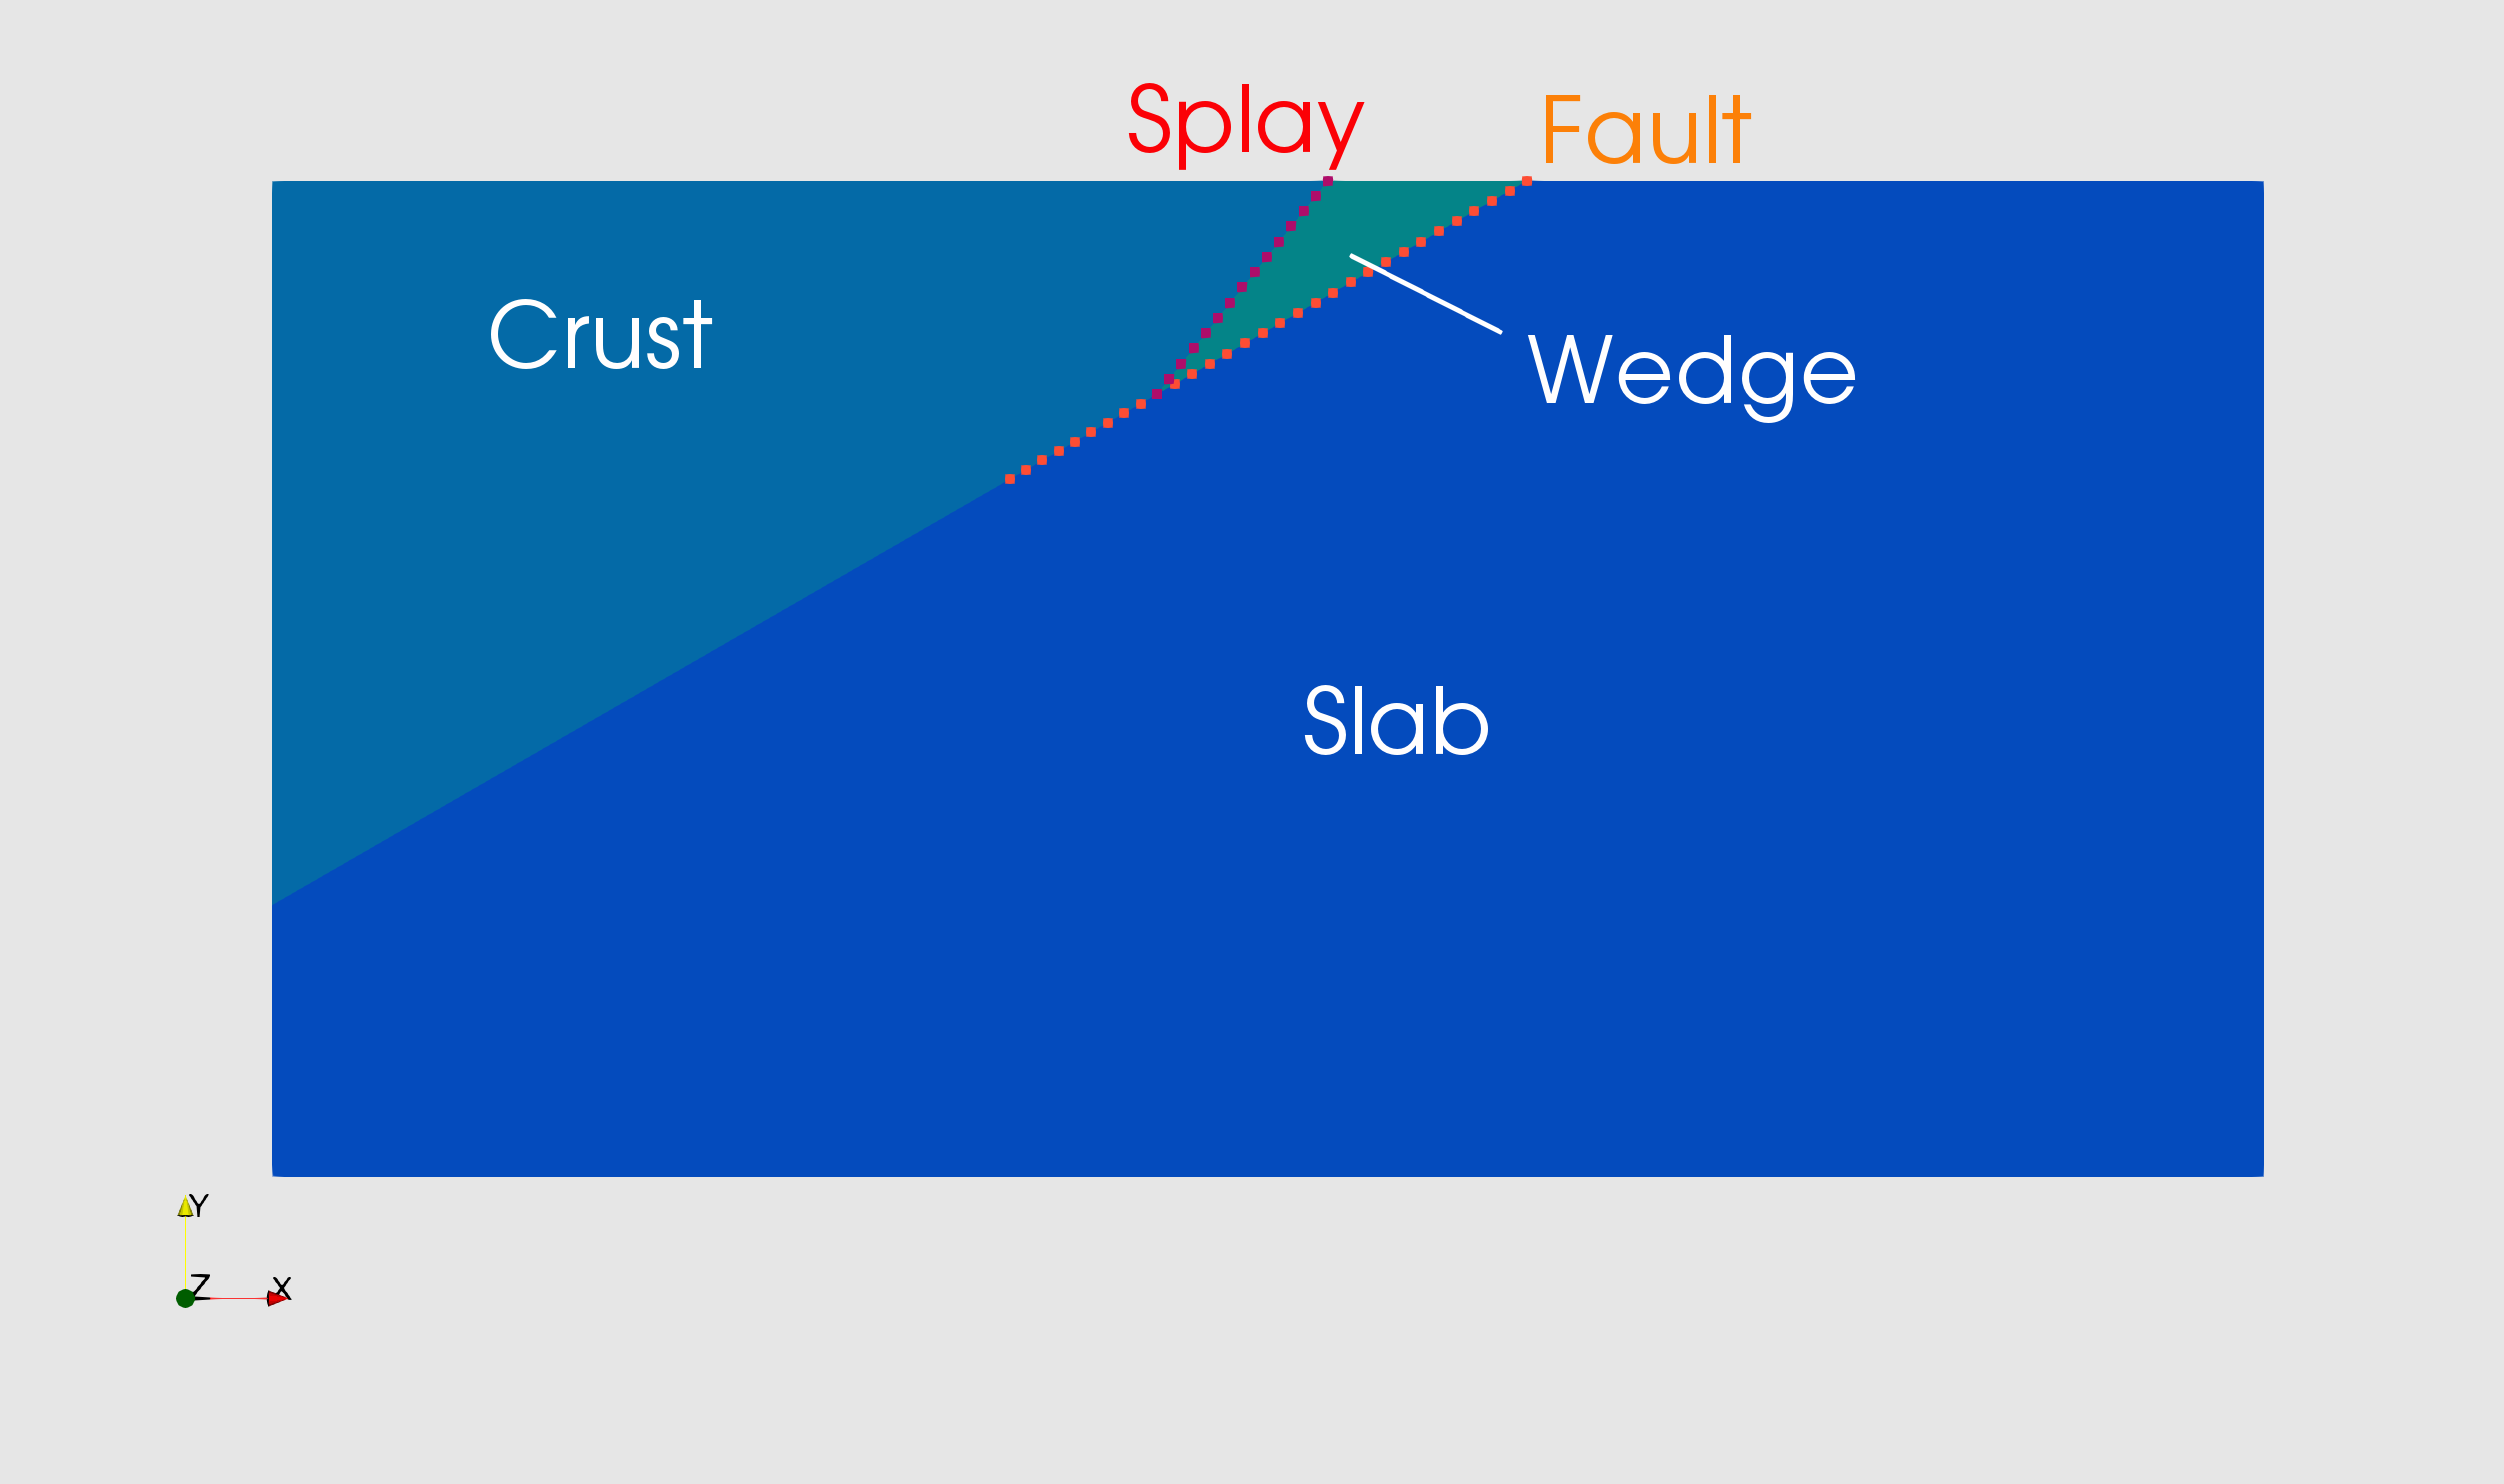
\includegraphics[width=4.5in]{examples/figs/reverse2d_geometry}
  \caption{Geometry used for 2D reverse fault example.}
  \label{fig:example:reverse:2d:geometry}
\end{figure}

Note that although we label the different parts of the mesh as slab,
crust, and wedge, the actual thrust fault only extends 60 km downdip,
and we do not provide bottom boundaries for the crust and slab.
The files associated with this suite of examples are contained in the
directory \filename{examples/2d/reverse}. This directory contains
several files:
\begin{description}
\item[\filename{*.jou}] Files used to construct the finite-element mesh using
  CUBIT/Trelis.
\item[\filename{*.spatialdb}] Files associated with the spatial databases.
\item[\filename{viz}] Directory containing ParaView
  Python scripts and other files for visualizing results.
\item[\filename{output}] Directory containing simulation
  output. It is created automatically when running the
  simulations.
\item[\filename{README.md}] README file containing a brief description
  of the various examples.
\end{description}


% ----------------------------------------------------------------------
\subsection{Features Illustrated}

Table~\ref{tab:example:reverse:2d:features} lists the features
discussed in each of these 2-D reverse fault examples. With the
intent of illustrating features used in research simulations, we use
HDF5 output and we make extensive use the most efficient
implementations of spatial databases (UniformDB and ZeroDB). We
also use ParaView Python scripts for visualizing the output. These
scripts can be run within the ParaView GUI or outside the ParaView
GUI, although the interaction is limited to rotating, translating, and
zooming when run outside the ParaView GUI.

\begin{table}[htbp]
  \caption{PyLith features covered in the suite of 2-D reverse fault examples.}
  \label{tab:example:reverse:2d:features}
  \input{examples/2d_reverse_features}
\end{table}

% ----------------------------------------------------------------------
\subsection{Generating the Finite-Element Mesh}

We use CUBIT/Trelis to generate the finite-element mesh. Due to the
small size of these 2D meshes, we include them in the PyLith source
and binary distributions. If you do not have CUBIT/Trelis, you can
use the provided meshes.

Mesh generation is controlled from either \filename{mesh\_tri.jou}
(triangular meshes) or \filename{mesh\_quad.jou} (quadrilateral
meshes). In addition to creating the desired meshes, these scripts
call the following additional journal files:
\begin{description}
\item[\filename{geometry.jou}] Journal file to create the 2D geometry.
\item[\filename{gradient.jou}] Journal file to assign sizing
  information for the mesh.
\item[\filename{createbc.jou}] Journal file to define material blocks
  and nodesets for boundary conditions.
\end{description}

The first step is to create the geometry. This consists of creating a
brick, extracting a midsurface from it, and then splitting the
remaining surface with an extended fault and a splay surface. The
surfaces, curves, and important vertices are then assigned names that
are then used when setting up mesh sizing information and defining
blocks and nodesets.

\important{We use IDless journaling in CUBIT/Trelis. This allows us to
  reference objects in a manner that should be independent of the
  version of CUBIT/Trelis that is being used. In the journal files,
  the original command used is typically commented out, and the
  following command is the equivalent IDless command.}

Once the geometry has been generated, we then set sizing information
using both a user-defined sizing function as well as the CUBIT/Trelis
curve and surface bias schemes. Using this sizing information, an
initial mesh is generated, and then one iteration of smoothing is
performed to improve the cell quality. Finally, blocks are defined for
the three materials in the problem, and nodesets are also defined for
the fault and splay surfaces.

\important{In addition to providing nodesets for the fault and splay,
  it is also important to provide nodesets defining the buried edges
  of these two surfaces. In 2D, this will consist of a single vertex
  for each surface. This information is required by PyLith to form the
  corresponding cohesive cells defining fault surfaces.}

Once you have run either the \filename{mesh\_tri.jou} or
\filename{mesh\_quad.jou}journal file to construct the geometry and
generate the mesh, you will have a corresponding Exodus-II file
(\filename{mesh\_tri.exo} or \filename{mesh\_quad.exo}). These are
NetCDF files, and they can be loaded into ParaView.
%******* Finish fixing from here **********

\subsubsection{Visualizing the Mesh}

The Exodus-II file \filename{mesh\_tet.exo} can be viewed with
ParaView. We provide the Python script \filename{viz/pot\_mesh.py} to
visualize the nodesets and the mesh quality using the condition number
metric. As in our other Python scripts for ParaView (see
Section~\vref{sec:ParaView:Python:scripts} for a discussion of how to use
Python ParaView scripts), you can override the default
parameters by setting appropriate values in the Python shell (if
running within the ParaView GUI) or from the command line (if running
the script directly outside the GUI). When viewing the nodesets, the
animation controls allow stepping through the nodesets. When viewing
the mesh quality, only the cells with the given quality metric above
some threshold (poorer quality) are shown. The default quality metric
is condition number and the default threshold is 2.0.

To visualize the mesh, start ParaView. Within the ParaView GUI Python shell
(\menu{Tools}$\rightarrow$\menu{Python Shell}), we override the
\filename{EXODUS\_FILE} and \filename{SHOW\_QUALITY} parameters.
\begin{python}[ParaView Python shell]
# Import the os module so we can get access to the HOME environment variable.
>>> import os
>>> HOME = os.environ["HOME"]
# You may need to adjust the next line, depending on where you installed PyLith.
>>> EXODUS_FILE = os.path.join(HOME,"pylith","examples","3d","subduction","mesh","mesh_tet.exo")
# Turn off display of the mesh quality (show only the nodesets).
>>> SHOW_QUALITY = False
\end{python}
We then click on the \menu{Run Script} button and navigate to the
\filename{examples/3d/subduction/viz} directory and select
\filename{plot\_mesh.py}.

\begin{figure}[htbp]
  \includegraphics[width=5.0in]{examples/figs/subduction3d_mesh}
  \caption{Visualization of the \object{fault\_slabtop} nodeset
    (yellow dots) for the Exodus-II file \filename{mesh/mesh\_tet.exo}
    using the \filename{viz/plot\_mesh.py} ParaView Python script. One
    can step through the different nodesets using the animation
    controls. This script can also be use to show the mesh quality.}
  \label{fig:example:subduction:3d:mesh}
\end{figure}

\subsection{Organization of Simulation Parameters}
\label{sec:example:subduction:3d:organization}

PyLith automatically reads in \filename{pylithapp.cfg} from the
current directory, if it exists. As a result, we generally put all
parameters common to a set of examples in this file to avoid
duplicating parameters across multiple files. Because we often use a
single mesh for multiple simulations in a directory, we place all
parameters related to our mesh and identifying the materials in our
mesh in \filename{pylithapp.cfg}. We assign the bulk constitutive
model and its parameters to each material in other files, because we
vary those across the simulations. In general, we place roller
boundary conditions (Dirichlet boundary conditions constraining the
degrees of freedom perpendicular to the boundary) on the lateral and
bottom boundaries, so we include those in \filename{pylithapp.cfg}. In
some simulations we will overwrite the values for parameters will
values specific to a given example. This file is also a convenient
place to put basic solver parameters and to turn on Pyre journals for
displaying informational messages during a run.journalling debugging
flags.

Hence the settings contained in \filename{pylithapp.cfg} include:
\begin{inventory}
  \facilityitem{pylithapp.journal.info}{Settings that control the
    verbosity of the output written to stdout for the different
    components.}
  \facilityitem{pylithapp.mesh\_generator}{Parameters for the type of
    mesh importer (generator), reordering of the mesh, and the mesh
    coordinate system.}
  \facilityitem{pylithapp.problem.materials}{Basic parameters for each
    of the four materials, including the label, block id in the mesh
    file, discretization, and output writer.}
  \facilityitem{pylithapp.problem.bc}{Parameters for Dirichlet
    boundary conditions on the lateral and bottom boundaries of the
    domain.}
  \facilityitem{pylithapp.problem.formulation.output}{Settings related
    output of the solution over the domain and subdomain (ground
    surface).}
  \facilityitem{pylithapp.petsc}{PETSc solver and logging settings.}
\end{inventory}

\subsubsection{Coordinate system}

We generated the mesh in a Cartesian coordinate system corresponding
to a transverse Mercator projection. We specify this geographic
projection coordinate system in the \filename{pylithapp.cfg} file, so
that we can use other convenient georeferenced coordinate systems in
the spatial databases. PyLith will automatically transform points
between compatible coordinate systems. Our spatialdata library uses
Proj4 for geographic projections, so we specify the projection using
Proj4 syntax in the \property{proj\_options} property:
\begin{cfg}[Excerpt from \filename{pylithapp.cfg}]
<h>[pylithapp.mesh_generator.reader]</h>
<f>coordsys</f> = spatialdata.geocoords.CSGeoProj
<p>coordsys</p>.space_dim = 3
<p>coordsys</p>.datum_horiz = WGS84
<p>coordsys.datum_vert</p> = mean sea level
<p>coordsys.projector.projection</p> = tmerc
<p>coordsys.projector.proj_options</p> = +lon_0=-122.6765 +lat_0=45.5231 +k=0.9996
\end{cfg}

\subsubsection{Materials}

The finite-element mesh marks cells for each material and the type of
cell determines the type of basis functions we use in the
discretization. This means we can specify this information in the
\filename{pylithapp.cfg} file and avoid duplicating it in each
simulation parameter file. To set up the materials, we first create an
array of materials that defines the name for each material component.
For example, we create the array of four materials and then set the
parameters for the slab:
\begin{cfg}[Excerpt from \filename{pylithapp.cfg}]
<h>[pylithapp.problem]</h>
<f>materials</f> = [slab, wedge, crust, mantle]

<h>[pylithapp.problem.materials.slab]</h>
<p>label</p> = Subducting slab ; Label for informative error messages
<p>id</p> = 1 ; Block id in ExodusII file from CUBIT/Trelis
<f>quadrature.cell</f> = pylith.feassemble.FIATSimplex ; Tetrahedral cells
<p>quadrature.cell.dimension</p> = 3

# Average cell output over quadrature points, yielding one point per cell
<f>output.cell_filter</f> = pylith.meshio.CellFilterAvg
<f>output.writer</f> = pylith.meshio.DataWriterHDF5 ; Output using HDF5
\end{cfg}

In this set of examples, we will consider cases in which all materials
are linear, isotropic elastic and cases where the crust and wedge are
linear, isotropic elastic but the slab and mantle are linear Maxwell
viscoelastic. As a result, we put the parameters for these two cases
in separate \filename{cfg} files with \filename{mat\_elastic.cfg} for
the case with purely elastic models and
\filename{mat\_viscoelastic.cfg} for the case with a mix of elastic
and viscoelastic models. Each of these files specifies the bulk
constitutive model and spatial database to use for the properties for
each material. The values for the material properties are loosely
based on a 3-D seismic velocity model for the Pacific Northwest 
\cite{Stephenson:2007}.

\subsubsection{Boundary Conditions}

For the Dirichlet boundary conditions, we specify the degree of
freedom constrained, the name of the nodeset in the ExodusII file from
CUBIT/Trelis that defines the boundary, and a label for the spatial
database (required for informative error messages). These settings
constrain the y-displacement on the north (+y) boundary:
\begin{cfg}[Excerpt from \filename{pylithapp.cfg}]
<h>[pylithapp.problem.bc.y_pos]</h>
<p>bc_dof</p> = [1] ; Degree of freedoms are: x=0, y=1, and z=2
<p>label</p> = boundary_ypos ; nodeset in ExodusII file form CUBIT/Trelis
<p>db_initial.label</p> = Dirichlet BC on +y ; label for informative error messages
\end{cfg}

\subsubsection{Solver Parameters}

We group solver parameters into a few different files to handle
different cases. The \filename{pylithapp.cfg} contains tolerance
values for the linear and nonlinear solvers and turns on some simple
diagnostic information. The file also directs PyLith to use a direct
solver, which is suitable for debugging and test problems that do not
include a fault; a direct solver is not well-suited for production
runs because it does not scale well and uses a lot of memory.
\begin{cfg}[Excerpt from \filename{pylithapp.cfg}]
<h>[pylithapp.petsc]</h>
<p>malloc_dump</p> = ; Dump information about PETSc memory not deallocated.

# Use LU preconditioner (helpful for learning and debugging, not production simulations)
<p>pc_type</p> = lu

# Convergence parameters.
<p>ksp_rtol</p> = 1.0e-10 ; Converge if residual norm decreases by this amount
<p>ksp_atol</p> = 1.0e-11 ; Converge if residual norm drops below this value
<p>ksp_max_it</p> = 500 ; Maximum number of iterations in linear solve
<p>ksp_gmres_restart</p> = 50 ; Restart orthogonalization in GMRES after this number of iterations

# Linear solver monitoring options.
<p>ksp_monitor</p> = true ; Show residual norm at each iteration
#ksp_view = true ; Show solver parameters (commented out)
<p>ksp_converged_reason</p> = true ; Show reason linear solve converged
<p>ksp_error_if_not_converged</p> = true ; Generate an error if linear solve fails to converge

# Nonlinear solver monitoring options.
<p>snes_rtol</p> = 1.0e-10 ; Converge if nonlinear residual norm decreases by this amount
<p>snes_atol</p> = 1.0e-9 ; Converge if nonlinear residual norm drops below this value
<p>snes_max_it</p> = 100 ; Maximum number of iterations in nonlinear solve
<p>snes_monitor</p> = true ; Show nonlinear residual norm at each iteration
<p>snes_linesearch_monitor</p> = true ; Show nonlinear solver line search information
#snes_view = true ; Show nonlinear solver parameters (commented out)
<p>snes_converged_reason</p> = true ; Show reason nonlinear solve converged
<p>snes_error_if_not_converged</p> = true ; Generate an error if nonlinear solve fails to converge

# PETSc summary -- useful for performance information.
<p>log_view</p> = true
\end{cfg}

The
\filename{solver\_algebraicmultigrid.cfg} provides more optimal
settings for simulations without a fault by using an algebraic
multigrid preconditioner. Similarly, for simulations with a fault
\filename{solver\_fieldsplit.cfg} provides settings for applying the
algebraic multigrid preconditioner to the elasticity portion of the
system Jacobian matrix and our custom fault preconditioner to the
Lagrange multiplier portion.

% ----------------------------------------------------------------------
\subsection{Step 1: Axial Compression}
\label{sec:example:subduction:3d:step01}

We start with a very simple example of axial compression in the
east-west direction with purely elastic material properties, and no
faults (Figure~\ref{fig:example:subduction:3d:step01:diagram}). We
impose axial compression using Dirichlet boundary conditions on the
east (+x) and west (-x) boundaries and confine the domain in the
north-south direction via zero displacement Dirichlet boundary
conditions on the north (+y) and south (-y) boundaries.  We constrain
the vertical displacement by imposing zero displacement boundary
conditions on the bottom (-z) boundary.

\begin{figure}[htbp]
  \includegraphics[scale=0.75]{examples/figs/subduction3d_step01_diagram}
  \caption{Diagram of Step 1: Axial compression. This static
    simulation uses Dirichlet boundary conditions with axial
    compression in the east-west (x-direction), roller boundary
    conditions on the north, south, and bottom boundaries, and purely
    elastic properties.}
  \label{fig:example:subduction:3d:step01:diagram}
\end{figure}

The \filename{pylithapp.cfg} file creates an array of five boundary
conditions, which impose zero displacements by default. We overwrite
this behavior in the \filename{step01.cfg} file for the -x and +x
boundaries using spatial databases with a single uniform displacement
value to create the axial compression:
\begin{cfg}[Excerpt from \filename{step01.cfg}]
# -x face
<h>[pylithapp.problem.bc.x_neg]</h>
<f>db_initial</f> = spatialdata.spatialdb.UniformDB
<p>db_initial.label</p> = Dirichlet BC on -x
<p>db_initial.values</p> = [displacement-x]
<p>db_initial.data</p> = [+2.0*m]

# +x face
<h>[pylithapp.problem.bc.x_pos]</h>
<f>db_initial</f> = spatialdata.spatialdb.UniformDB
<p>db_initial.label</p> = Dirichlet BC on +x
<p>db_initial.values</p> = [displacement-x]
<p>db_initial.data</p> = [-2.0*m]
\end{cfg}

As discussed in Section~\vref{sec:example:subduction:3d:organization},
we use \filename{mat\_elastic.cfg} to specify the parameters
associated with linear, isotropic elastic bulk constitutive models for
all of the materials for convenient reuse across several different
simulations.
\begin{cfg}[Excerpt from \filename{mat\_elastic.cfg}]
<h>[pylithapp.problem.materials]</h>
<f>slab</f> = pylith.materials.ElasticIsotropic3D
<f>wedge</f> = pylith.materials.ElasticIsotropic3D
<f>crust</f> = pylith.materials.ElasticIsotropic3D
<f>mantle</f> = pylith.materials.ElasticIsotropic3D

# Slab
<h>[pylithapp.problem.materials.slab]</h>
<f>db_properties</f> = spatialdata.spatialdb.SimpleDB
<p>db_properties.label</p> = Properties for subducting slab
<p>db_properties.iohandler</p>.filename = spatialdb/mat_slab_elastic.spatialdb

# Wedge
<h>[pylithapp.problem.materials.wedge]</h>
<f>db_properties</f> = spatialdata.spatialdb.SimpleDB
<p>db_properties.label</p> = Properties for accretionary wedge
<p>db_properties.iohandler.filename</p> = spatialdb/mat_wedge_elastic.spatialdb

# Mantle
<h>[pylithapp.problem.materials.mantle]</h>
<f>db_properties</f> = spatialdata.spatialdb.SimpleDB
<p>db_properties.label</p> = Properties for mantle
<p>db_properties.iohandler.filename</p> = spatialdb/mat_mantle_elastic.spatialdb

# Crust
<h>[pylithapp.problem.materials.crust]</h>
<f>db_properties</f> = spatialdata.spatialdb.SimpleDB
<p>db_properties.label</p> = Properties for continental crust
<p>db_properties.iohandler.filename</p> = spatialdb/mat_crust_elastic.spatialdb
\end{cfg}
We specify different elastic properties for each material
(slab, wedge, mantle, and crust) using \object{SimpleDB} spatial
databases with a single point to specify uniform properties within a
material. We choose \object{SimpleDB} rather than \object{UniformDB},
because we will reuse some of these spatial databases for the elastic
properties when we use linear Maxwell viscoelastic constitutive model.

The remaining parameters in the \filename{step01.cfg} file are mostly
associated with setting filenames for all of the various output,
including all of the parameters used and version information in a JSON
file (\filename{output/step01-parameters.json}), a file reporting the
progress of the simulation and estimated time of completion
(\filename{output/step01-progress.txt}), and the filenames for the
HDF5 files (the corresponding Xdmf files will use the same filename
with the \filename{xmf} suffix).

\begin{shell}[Run Step 1 simulation]
$ pylith step01.cfg mat_elastic.cfg
\end{shell}
The simulation will produce ten pairs of HDF5/Xdmf files in the
\filename{output} directory:
\begin{description}
% Domain and subdomain output
\item[\filename{step01-domain.h5[.xmf]}] Time series of the solution field over the domain.
\item[\filename{step01-groundsurf.h5[.xmf]}] Time series of the solution field over the ground surface.
% Materials
\item[\filename{step01-slab\_info.h5[.xmf]}] Properties for
  the slab material.
\item[\filename{step01-slab.h5[.xmf]}] Time series of the state variables (stress and strain) for the slab material.
\item[\filename{step01-wedge\_info.h5[.xmf]}] Properties for
  the wedge material.
\item[\filename{step01-wedge.h5[.xmf]}] Time series of the state variables (stress and strain) for the wedge material.
\item[\filename{step01-crust\_info.h5[.xmf]}] Properties for
  the crust material.
\item[\filename{step01-crust.h5[.xmf]}] Time series of the tate variables
  (stress and strain) for the crust material.
\item[\filename{step01-mantle\_info.h5[.xmf]}] Properties for
  the mantle material.
\item[\filename{step01-mantle.h5[.xmf]}] Time series of the state variables
  (stress and strain) for the mantle material.
\end{description}
The HDF5 files contain the data and the Xdmf files contain the
metadata required by ParaView and Visit (and other visualization tools
that use Xdmf files) to access the mesh and data sets in the HDF5
files.

Figure \ref{fig:example:subduction:3d:step01}, which was created using
the ParaView Python script \filename{plot\_dispvec.py} (see
Section~\vref{sec:ParaView:Python:scripts} for how to run ParaView
Python scripts), displays the magnitude of
the displacement field arrows showing the direction and magnitude of
the deformation. Material properties with a positive Poisson's ratio
result in vertical deformation along with the axial compression. The
variations in material properties among the properties result in local
spatial variations that are most evident in the horizontal
displacement components.

\begin{figure}
  \includegraphics[width=5.0in]{examples/figs/subduction3d_step01_soln}
  \caption{Solution over the domain for Step 1. The colors indicate
    the magnitude of the displacement and the arrows indicate the
    direction with the length of each arrow equal to 10,000 times the
    magnitude of the displacement.}
  \label{fig:example:subduction:3d:step01}
\end{figure}

\subsubsection{Exercises}

\begin{itemize}
\item Run PyLith again and add
  \filename{solver\_algebraicmultigrid.cfg} as an argument on the
  command line to switch to the algebraic multigrid preconditioner.
  \begin{itemize}
  \item Using the PETSc log summary to compare the runtime and memory
    use between the original LU preconditioner and the ML algebraic
    multigrid preconditioner. Hint: The algebraic multigrid
    preconditioner is faster.
  \item Run the simulation again with the algebraic multigrid
    preconditioner using multiple cores via the
    \commandline{-{}-nodes=NCORES} argument, replacing
    \commandline{NCORES} with 2 or up to the number of cores on your
    machine. Examine the PETSc log summary for the various runs to see
    how the time spent at varies stages changes with the number of
    cores. Make a plot of runtime versus the number of cores.
  \end{itemize}
\item Adjust the material properties in the spatial databases so that
  the slab is stiffer and the wedge is more compliant. What happens to
  the solution if you make the materials nearly incompressible? Does
  this also affect the rate of convergence of the linear solve?
\item Change the Dirichlet boundary conditions to impose pure shear
  instead of axial compression. Hint: You will need to change the
  boundary conditions on the east, west, north, and south boundaries.
\end{itemize}
    

% ----------------------------------------------------------------------
\subsection{Step 2: Prescribed Coseismic Slip and Postseismic Relaxation}
\label{sec:example:subduction:3d:step02}

In this example we model the postseismic relaxation of the deep slab
and mantle resulting from coseismic slip on a fault patch in the
central portion of the subduction (top of the slab) interface. For
simplicity we will prescribed uniform slip on the fault patch and use
a linear Maxwell viscoelastic constitutive models for the slab and
mantle. As the lateral and bottom boundaries are far from the
earthquake source, we use roller boundary conditions on these
boundaries. We do not expect significant relaxation of stresses on the
shallow part of the slab, so we impose a depth-dependent
viscosity. Figure~\ref{fig:example:subduction:3d:step02:diagram}
summarizes the problem description.

\begin{figure}[htbp]
  \includegraphics[scale=0.75]{examples/figs/subduction3d_step02_diagram}
  \caption{Diagram of Step 2: Prescribed coseismic slip and
    postseismic relaxation. This quasistatic simulation prescribes
    uniform slip on the central rupture patch on the subduction interface,
    depth-dependent viscoelastic relaxation in the slab and mantle,
    and roller boundary conditions on the lateral (north, south, east,
    and west) and bottom boundaries.}
  \label{fig:example:subduction:3d:step02:diagram}
\end{figure}

The \filename{pylithapp.cfg} completely specifies the Dirichlet roller
boundary conditions on the five boundaries, so we do not include any
boundary condition information in \filename{step02.cfg}. As discussed
in Section~\vref{sec:example:subduction:3d:organization}, we bundle
the parameters for specification of an elastic crust and wedge and
viscoelastic slab and mantle in \filename{mat\_viscoelastic.cfg}.

% Materials
We describe the properties of the linear, isotropic Maxwell
viscoelastic constitutive model using viscosity in addition to the Vp,
Vs, and density used to describe purely linear, isotropic elastic
models. Rather than create a database with all four of these
parameters, we leverage the \object{SimpleDB} spatial databases used
by \filename{mat\_elastic.cfg} for the elastic properties and simply
create a single new spatial database with the depth-dependent
viscosity for the slab and mantle. We use the \object{CompositeDB}
spatial database to combine these two spatial databases into a single
spatial database with the material properties. Rather than using a
\object{SimpleDB} for the depth-dependent viscosity, we use a
\object{SimpleGridDB} spatial database
(\filename{spatialdb/mat\_viscosity}), which provides faster
interpolation using a bilinear search algorithm along each coordinate
direction. We use a very large viscosity at depths above 20 km to give
behavior that is essentially elastic and decrease it so the Maxwell
relaxation time (viscosity divided by the shear modulus) is
approximately 200 years at a depth of 30 km, 100 years at a depth of
100 km, and 50 years at a depth of 400 km. Using linear interpolation
results in a piecewise linear variation in the viscosity with depth.

\tip{The \object{SimpleGridDB} should be used whenever the points in a
  spatial database can be described with a logically rectangular
  grid. The grid points along each direction do not need to be
  uniformly spaced.}

In setting the parameters for the \object{CompositeDB} in
\filename{mat\_viscoelastic.cfg}, we specify which properties are
contained in each of the two spatial databases in the composite
database and the type and parameters for each of those spatial
databases. For the slab we have:
\begin{cfg}[Excerpt from \filename{mat\_viscoelastic.cfg}]
<h>[pylithapp.problem.materials.slab]</h>
<f>db_properties</f> = spatialdata.spatialdb.CompositeDB
<p>db_properties.label</p> = Composite spatial database for slab material properties

<h>[pylithapp.timedependent.materials.slab.db_properties]</h>
# Elastic properties
<p>values_A</p> = [density, vs, vp]
<f>db_A</f> = spatialdata.spatialdb.SimpleDB
<p>db_A.label</p> = Elastic properties
<p>db_A.iohandler.filename</p> = spatialdb/mat_slab_elastic.spatialdb

# Viscoelastic properties
<p>values_B</p> = [viscosity]
<f>db_B</f> = spatialdata.spatialdb.SimpleGridDB
<p>db_B.label</p> = Linear Maxwell viscoelastic properties
<p>db_B.filename</p> = spatialdb/mat_viscosity.spatialdb
<p>db_B.query_type</p> = linear
\end{cfg}

In the simulation specific parameter file \filename{step02.cfg}, we
specify the parameters for the quasistatic time stepping, the
coseismic rupture, and the filenames for output. By default, PyLith
will use implicit time stepping with uniform time steps, so we need
only specify the duration and time step size.
\begin{cfg}[Excerpt from \filename{step02.cfg}]
<h>[pylithapp.problem.formulation.time_step]</h>
# Define the total time for the simulation and the time step size.
<p>total_time</p> = 200.0*year
<p>dt</p> = 10.0*year
\end{cfg}

In prescribing coseismic slip on the single fault patch, we create an
array with one fault interface and then set its parameters. Because
the edges of the central fault patch are buried within the domain, we
need to specify the nodeset that corresponds to the buried edges as
well as the nodeset for the entire fault surface. This ensures that
PyLith inserts the cohesive cells and properly terminates the fault
surface at the edges. Just as we do for the boundary conditions and
materials, we create an array of components (in this case an array
with one fault interface, \facility{slab}, and then refer to those
components by name, \facility{pylithapp.problem.interfaces.slab}. We
must also set the discretization information for the fault.
\begin{cfg}[Excerpt from \filename{step02.cfg}]
<h>[pylithapp.problem]</h>
# We prescribe slip on the slab fault patch.
<f>interfaces</f> = [slab]

<h>[pylithapp.problem.interfaces]</h>
<f>slab</f> = pylith.faults.FaultCohesiveKin ; Default

<h>[pylithapp.problem.interfaces.slab]</h>
<p>label</p> = fault_slabtop_patch ; Nodeset for entire fault surface
<p>edge</p> = fault_slabtop_patch_edge ; Nodeset for buried edges

# We must define the quadrature information for fault cells.
# The fault cells are 2D (surface).
<f>quadrature.cell</f> = pylith.feassemble.FIATSimplex
<p>quadrature.cell.dimension</p> = 2
\end{cfg}

Prescribing the coseismic slip distribution on the fault involves
specifying an origin time for the rupture (default is 0.0), and a slip
time function along with its parameters. In this case, we treat the
earthquake rupture as just the coseismic slip happening in one time
step, so we use a step function for the slip time function (which is
the default). The parameters include the final slip and slip
initiation time. This slip initiation time is relative to the
earthquake source origin time, which is 0 by default. Thus, to specify
the time of the slip for a step function, we can either specify the
origin time or the slip initiation time; in this case, we use the slip
initiation time. In Step 4 we will use the origin time. Because we
want uniform slip and a uniform rise time, we use \object{UniformDB}
spatial databases for both of these. Note that we specify oblique slip
with 1.0 m of right-lateral motion and 4.0 m of reverse motion.
\begin{cfg}[Excerpt from \filename{step02.cfg}]
<h>[pylithapp.problem.interfaces.slab.eq_srcs.rupture.slip_function]</h>
<f>slip</f> = spatialdata.spatialdb.UniformDB
<p>slip.label</p> = Final slip
<p>slip.values</p> = [left-lateral-slip, reverse-slip, fault-opening]
<p>slip.data</p> = [-1.0*m, 4.0*m, 0.0*m] 

<f>slip_time</f> = spatialdata.spatialdb.UniformDB
<p>slip_time.label</p>  = Slip initiation time
<p>slip_time.values</p> = [slip-time]
<p>slip_time.data</p> = [9.999*year] ; Use 10*year-small value to account for roundoff errors

<h>[pylithapp.problem.interfaces.slab.output]</h>
<f>writer</f> = pylith.meshio.DataWriterHDF5
<p>writer.filename</p> = output/step02-fault-slab.h5
<p>vertex_info_fields</p> = [normal_dir, strike_dir, dip_dir, final_slip_rupture, slip_time_rupture]
\end{cfg}

\begin{shell}[Run Step 2 simulation]
$ pylith step02.cfg mat_viscoelastic.cfg solver_fieldsplit.cfg
\end{shell}
In addition to the ten pairs of HDF5/Xdmf files analogous to those
produced in Step 1, we also have two pairs of HDF5/Xdmf files
associated with the fault:
\begin{description}
% Domain and subdomain output
\item[\filename{step02-domain.h5[.xmf]}] Time series of the solution field over the domain.
\item[\filename{step02-groundsurf.h5[.xmf]}] Time series of the solution field over the ground surface.
% Materials
\item[\filename{step02-slab\_info.h5[.xmf]}] Properties for
  the slab material.
\item[\filename{step02-slab.h5[.xmf]}] Time series of the state variables (stress and strain) for the slab material.
\item[\filename{step02-wedge\_info.h5[.xmf]}] Properties for
  the wedge material.
\item[\filename{step02-wedge.h5[.xmf]}] Time series of the state variables (stress and strain) for the wedge material.
\item[\filename{step02-crust\_info.h5[.xmf]}] Properties for
  the crust material.
\item[\filename{step02-crust.h5[.xmf]}] Time series of the tate variables
  (stress and strain) for the crust material.
\item[\filename{step02-mantle\_info.h5[.xmf]}] Properties for
  the mantle material.
\item[\filename{step02-mantle.h5[.xmf]}] Time series of the state variables
  (stress and strain) for the mantle material.
% Fault
\item[\filename{step02-fault-slab\_info.h5[.xmf]}] Fault orientation
  and rupture information.
\item[\filename{step02-fault-slab.h5[.xmf]}] Time series of slip and
  traction changes.
\end{description}

Figure \ref{fig:example:subduction:3d:step02}, which was created
using the ParaView Python script \filename{plot\_dispwarp.py},
displays the magnitude of the displacement field exaggerated by a
factor of 10,000 at the final time step (200 yr).  The shallow
fault results in deformation that is localized over a small region.

\begin{figure}
  \includegraphics[width=5.0in]{examples/figs/subduction3d_step02_soln}
  \caption{Solution over the domain for Step 2 at $t = 200 \mathrm{yr}$. The
    colors indicate the magnitude of the displacement and we have
    exaggerated the deformation by a factor of 10,000.}
  \label{fig:example:subduction:3d:step02}
\end{figure}


\subsubsection{Exercises}

\begin{itemize}
\item Change the slip from the subduction interface rupture patch to
  the splay fault rupture patch. Hint: Identify the nodesets for the
  splay fault patch.
\item Create simultaneous rupture on the subduction interface rupture
  patch and the splay fault rupture patch.
\item Prescribe coseismic slip on the central patch for splay fault
  and the subduction interface below the intersection with the splay fault.
  \begin{itemize}
  \item Implement this without changing any of the nodesets in
    CUBIT/Trelis. Hint: you will need to create two fault
    interfaces. What do you notice about the slip at the intersection
    between the splay fault and slab?
  \item Add nodesets in CUBIT/Trelis to create a uniform coseismic
    slip distribution across the splay fault and on the subduction interface
    below the splay fault.
  \end{itemize}
\end{itemize}


% ----------------------------------------------------------------------
\subsection{Step 3: Prescribed Aseismic Creep and Interseismic Deformation}
\label{sec:example:subduction:3d:step03}

We now increase the complexity of our fault model by simulating the
interseismic deformation associated with the subducting slab. We
approximate the motion of the Juan de Fuca Plate subducting under the
North American Plate by introducing aseismic slip (creep) on the
bottom of the slab and the deeper portion of the subduction interface;
we keep the interface between the subduction interface and the
accretionary wedge and shallow crust locked. As in Step 2, we will use
the linear Maxwell viscoelastic constitutive model for the slab and
mantle.  Figure~\ref{fig:example:subduction:3d:step03:diagram}
summarizes the problem description.

\begin{figure}[htbp]
  \includegraphics[scale=0.75]{examples/figs/subduction3d_step03_diagram}
  \caption{Diagram of Step 3: Prescribed aseismic slip (creep) and
    interseismic deformation for the subducting slab. We prescribe
    steady, uniform creep on the bottom of the slab and deeper portion
    of the subduction interface. We impose roller Dirichlet boundary
    conditions on the lateral and bottom boundaries, except where they
    overlap with the slab and splay fault.}
  \label{fig:example:subduction:3d:step03:diagram}
\end{figure}

% Fault
With slip on the top and bottom of the slab, our fault interfaces
array contains two components, one for the top of the slab (subduction
interface), \facility{slab\_top}, and one for the bottom of the slab,
\facility{slab\_bottom}. We use the \object{FaultCohesiveKin} object
for each of these interfaces since we want to prescribe the slip.
\begin{cfg}[Excerpt from \filename{step03.cfg}]
<h>[pylithapp.problem]</h>
<f>interfaces</f> = [slab_bottom, slab_top]

<h>[pylithapp.problem.interfaces]</h>
<f>slab_bottom</f> = pylith.faults.FaultCohesiveKin
<f>slab_top</f> = pylith.faults.FaultCohesiveKin
\end{cfg}

% Bottom of slab
We specify the \property{id} used to identify the cohesive cells for
this fault so that it is unique among all materials and faults. We
also specify the appropriate nodesets identifying the entire fault
surface and the buried edges.  Some portions of the bottom of the slab
are perfectly horizontal, so our procedure that uses the vertical
direction and the fault normal to set the along-strike and up-dip
shear components breaks down. We remedy this by tweaking the
\property{up\_dir} direction from being completely vertical (0,0,1) to
tilting slightly to the west. This results in consistent along-strike
and up-dip directions across the fault surface. For the aseismic slip
we use a constant slip rate time function (\object{ConstRateSlipFn})
with \object{UniformDB} spatial databases to specify the constant,
uniform oblique slip rate of 2.0 cm/yr of left-lateral motion and 4.0
cm/yr of normal motion. Note that slip on the bottom of the subducting
slab has the opposite sense of motion as that on the top of the slab.
\begin{cfg}[Excerpt from \filename{step03.cfg}]
<h>[pylithapp.problem.interfaces.slab_bottom]</h>
<p>id</p> = 100 ; Must be different from ids used for materials
<p>label</p> = fault_slabbot ; Nodeset for the entire fault surface
<p>edge</p> = fault_slabbot_edge ; Nodeset for the buried edges
# Give slight westward tilt to the up_dir to avoid ambiguous
# directions for the shear components on the horizontal portions of the
# fault.
<p>up_dir</p> = [-0.1,0,0.9]

# We must define the quadrature information for fault cells.
# The fault cells are 2D (surface).
<f>quadrature.cell</f> = pylith.feassemble.FIATSimplex
<p>quadrature.cell.dimension</p> = 2

# Use the constant slip rate time function.
<f>eq_srcs.rupture.slip_function</f> = pylith.faults.ConstRateSlipFn

# The slip time and final slip are defined in spatial databases.
<h>[pylithapp.problem.interfaces.slab_bottom.eq_srcs.rupture.slip_function]</h>
<f>slip_rate</f> = spatialdata.spatialdb.UniformDB
<p>slip_rate.label</p> = Slab bottom slip rate.
<p>slip_rate.values</p> = [left-lateral-slip, reverse-slip, fault-opening]
<p>slip_rate.data</p> = [+2.0*cm/year, -4.0*cm/year, 0.0*cm/year]

<f>slip_time</f> = spatialdata.spatialdb.UniformDB
<p>slip_time.label</p>  = Slip initiation time
<p>slip_time.values</p> = [slip-time]
<p>slip_time.data</p> = [0.0*year] 

<h>[pylithapp.problem.interfaces.slab_bottom.output]</h>
<f>writer</f> = pylith.meshio.DataWriterHDF5
<p>writer.filename</p> = output/step03-fault-slabbot.h5
<p>vertex_info_fields</p> = [normal_dir, strike_dir, dip_dir]
\end{cfg}

% Top of slab
The parameters for the top of the slab (subduction interface) closely
resemble those for the bottom of the slab. The main difference is that
we use a \object{SimpleGridDB} to define a depth variation in the slip
rate. The fault is locked at depths above 45 km and increases linearly
to the same slip rate as the bottom of the slab at a depth of 60 km.
\begin{cfg}[Excerpt from \filename{step03.cfg}]
<h>[pylithapp.problem.interfaces.slab_top]</h>
<p>id</p> = 101 ; Must be different from ids used for materials
<p>label</p> = fault_slabtop ; Nodeset for the entire fault surface
<p>edge</p> = fault_slabtop_edge ; Nodeset for the buried edges

# We must define the quadrature information for fault cells.
# The fault cells are 2D (surface).
<f>quadrature.cell</f> = pylith.feassemble.FIATSimplex
<p>quadrature.cell.dimension</p> = 2

# Use the constant slip rate time function.
<f>eq_srcs.rupture.slip_function</f> = pylith.faults.ConstRateSlipFn

# The slip time and final slip are defined in spatial databases.
<h>[pylithapp.problem.interfaces.slab_top.eq_srcs.rupture.slip_function]</h>
<f>slip_rate</f> = spatialdata.spatialdb.SimpleGridDB
<p>slip_rate.label</p> = Slab top slip rate.
<p>slip_rate.filename</p> = spatialdb/fault_slabtop_creep.spatialdb
<p>slip_rate.query_type</p> = linear

<f>slip_time</f> = spatialdata.spatialdb.UniformDB
<p>slip_time.label</p>  = Slip initiation time
<p>slip_time.values</p> = [slip-time]
<p>slip_time.data</p> = [0.0*year]

<h>[pylithapp.problem.interfaces.slab_top.output]</h>
<f>writer</f> = pylith.meshio.DataWriterHDF5
<p>writer.filename</p> = output/step03-fault-slabtop.h5
<p>vertex_info_fields</p> = [normal_dir, strike_dir, dip_dir]
\end{cfg}

% Boundary conditions
We do not want the boundaries to constrain the motion of the
subducting slab, so we use the nodesets that exclude vertices on the
subducting slab. Furthermore, PyLith does not permit overlap between
the fault interfaces and Dirichlet boundary conditions. This is why
we exclude vertices on the splay fault in these nodesets as well. We
only update the name of the nodeset for the -x, -y, and +y
boundaries.
\begin{cfg}[Excerpt from \filename{step03.cfg}]
# -x face
<h>[pylithapp.problem.bc.x_neg]</h>
<p>label</p> = boundary_xneg_noslab

# -y face
<h>[pylithapp.problem.bc.y_neg]</h>
<p>label</p> = boundary_yneg_noslab

# +y face
<h>[pylithapp.problem.bc.y_pos]</h>
<p>label</p> = boundary_ypos_noslab
\end{cfg}

\begin{shell}[Run Step 3 simulation]
$ pylith step03.cfg mat_viscoelastic.cfg solver_fieldsplit.cfg
\end{shell}
The simulation will produce fourteen pairs of HDF5/Xdmf files,
beginning with \filename{step03}, in the \filename{output}
directory:
\begin{description}
% Domain and subdomain output
\item[\filename{step03-domain.h5[.xmf]}] Time series of the solution field over the domain.
\item[\filename{step03-groundsurf.h5[.xmf]}] Time series of the solution field over the ground surface.
% Materials
\item[\filename{step03-slab\_info.h5[.xmf]}] Properties for
  the slab material.
\item[\filename{step03-slab.h5[.xmf]}] Time series of the state variables (stress and strain) for the slab material.
\item[\filename{step03-wedge\_info.h5[.xmf]}] Properties for
  the wedge material.
\item[\filename{step03-wedge.h5[.xmf]}] Time series of the state variables (stress and strain) for the wedge material.
\item[\filename{step03-crust\_info.h5[.xmf]}] Properties for
  the crust material.
\item[\filename{step03-crust.h5[.xmf]}] Time series of the tate variables
  (stress and strain) for the crust material.
\item[\filename{step03-mantle\_info.h5[.xmf]}] Properties for
  the mantle material.
\item[\filename{step03-mantle.h5[.xmf]}] Time series of the state variables
  (stress and strain) for the mantle material.
% Fault
\item[\filename{step03-fault-slabbot\_info.h5[.xmf]}] Fault orientation
  and rupture information for the bottom of the slab.
\item[\filename{step03-fault-slabbot.h5[.xmf]}] Time series of slip and
  traction changes for the bottom of the slab.
\item[\filename{step03-fault-slabtop\_info.h5[.xmf]}] Fault orientation
  and rupture information for the top of the slab.
\item[\filename{step03-fault-slabtop.h5[.xmf]}] Time series of slip and
  traction changes for the top of the slab.
\end{description}
As in Step 2, there are two pairs of HDF5/Xdmf files for
each fault; one set for the fault orientation and rupture information
and one set for the time series of slip and change in tractions.

Figure \ref{fig:example:subduction:3d:step03}, which was created
using the ParaView Python script \filename{plot\_dispwarp.py}, shows
the deformation exaggerated by a factor of 5,000 at the final time
step of t=200*yr. Notice that there are some local edge effects
associated with the unconstrained degrees of freedom at the
intersection of the boundaries and fault surfaces.

\begin{figure}
  \includegraphics[width=5.0in]{examples/figs/subduction3d_step03_soln}
  \caption{Solution over the domain for Step 2 at $t=200 \mathrm{yr}$. The colors indicate
    the x-displacement and we have exaggerated the
    deformation by a factor of 5,000.}
  \label{fig:example:subduction:3d:step03}
\end{figure}


\subsubsection{Exercises}

\begin{itemize}
\item Adjust the locking depth for the subduction interface. How does this
  affect the spatial distribution of the change in tractions on
  the fault interfaces?
\item Increase the rigidity of the slab and decrease the rigidity of
  the wedge and/or crust. How do these affect the change in tractions
  on the fault interfaces?
\end{itemize}


% ----------------------------------------------------------------------
\subsection{Step 4: Prescribed Earthquake Cycle}

In Step 4, We combine the interseismic deformation in Step 3 with the
coseismic slip in Step 2 to simulate two earthquake cycles. We also
include an earthquake on the splay fault. This illustrates how to
include multiple earthquake sources on a single fault. We use the same
roller Dirichlet boundary conditions and combination of elastic and
viscoelastic materials as we did in Step 3.

\begin{figure}[htbp]
  \includegraphics[scale=0.75]{examples/figs/subduction3d_step04_diagram}
  \caption{Diagram of Step 4: A simple earthquake cycle combining the
    prescribed aseismic slip (creep) from Step 3 with prescribed
    coseismic slip for two earthquakes on the shallow portion of the
    subduction interface and one earthquake on the play fault. We
    impose roller Dirichlet boundary conditions on the lateral and
    bottom boundaries, except where they overlap with the slab and
    splay fault.}
  \label{fig:example:subduction:3d:step04:diagram}
\end{figure}

% Faults
We create an array of three fault interfaces, one for the top of the
slab (subduction interface), one for the bottom of the slab, and one
for the splay fault. The splay fault terminates into the fault on the
top of the slab, so we must list the through-going fault on the top of
the slab first.
\begin{cfg}[Excerpt from \filename{step04.cfg}]
# We prescribe slip on the top and bottom of the slab and on the splay fault.
<h>[pylithapp.problem]</h>
<f>interfaces</f> = [slab_top, slab_bottom, splay]

<h>[pylithapp.problem.interfaces]</h>
<f>slab_top</f> = pylith.faults.FaultCohesiveKin
<f>slab_bottom</f> = pylith.faults.FaultCohesiveKin
<f>splay</f> = pylith.faults.FaultCohesiveKin
\end{cfg}

\important{When including intersecting faults, the through-going fault
  must be listed first in the array of fault interfaces. This ensures
  its cohesive cells are created before the adjacent fault that
  terminates into the through-going fault. For nonintersecting faults,
  the order in the list of fault interfaces does not matter.}

% Fault: slab_bottom and slab top
The settings for the fault interface on the bottom of the slab match
those used in Step 3. For the subduction interface, we want to
impose creep on the deeper portion and earthquakes (coseismic slip) at
specific times on the upper portion. We create an array of earthquake
sources, one for the creep and one for each of the earthquakes. We
want the earthquake to be imposed at specific times, so we set their
origin time equal to the desire rupture time (100 years and 200 years)
minus a value much smaller than the time step, so that roundoff errors
do not result in the ruptures occurring one time step later than
intended.  We use the same settings as we did in Step 3 for the creep
earthquake source. For the coseismic slip, we use a
\object{SimpleGridDB} to impose a depth-dependent slip distribution
that exactly complements the depth-dependent slip distribution of the
creep. Note that the slip time within an earthquake rupture is
relative to the origin time, so we set the slip time to zero to
coincide with the specified origin time.
\begin{cfg}[Excerpt from \filename{step04.cfg}]
[pylithapp.problem.interfaces.slab_top]
# --- Skipping lines already discussed in Step 3 ---
<f>eq_srcs</f> = [creep, eq1, eq2]
<p>eq_srcs.creep.origin_time</p> = 0.0*year
<p>eq_srcs.eq1.origin_time</p> = 99.999*year ; 100*yr - small value
<p>eq_srcs.eq2.origin_time</p> = 199.999*year l 200*yr - small value

# Use the constant slip rate time function for the creep earthquake source.
<f>eq_srcs.creep.slip_function</f> = pylith.faults.ConstRateSlipFn

# Creep
<h>[pylithapp.problem.interfaces.slab_top.eq_srcs.creep.slip_function]</h>
<f>slip_rate</f> = spatialdata.spatialdb.SimpleGridDB
<p>slip_rate.label</p> = Slab top slip rate.
<p>slip_rate.filename</p> = spatialdb/fault_slabtop_creep.spatialdb
<p>slip_rate.query_type</p> = linear

<f>slip_time</f> = spatialdata.spatialdb.UniformDB
<p>slip_time.label</p>  = Slip initiation time
<p>slip_time.values</p> = [slip-time]
<p>slip_time.data</p> = [0.0*year] ; Slip time is relative to origin time

# Earthquake 1
<h>[pylithapp.problem.interfaces.slab_top.eq_srcs.eq1.slip_function]</h>
<f>slip</f> = spatialdata.spatialdb.SimpleGridDB
<p>slip.label</p> = Slab top slip rate.
<p>slip.filename</p> = spatialdb/fault_slabtop_coseismic.spatialdb
<p>slip.query_type</p> = linear

<f>slip_time</f> = spatialdata.spatialdb.UniformDB
<p>slip_time.label</p>  = Slip initiation time
<p>slip_time.values</p> = [slip-time]
<p>slip_time.data</p> = [0.0*year] ; Slip time is relative to origin time.

# Earthquake 2 (same as earthquake 1)
<h>[pylithapp.problem.interfaces.slab_top.eq_srcs.eq2.slip_function]</h>
<f>slip</f> = spatialdata.spatialdb.SimpleGridDB
<p>slip.label</p> = Slab top slip rate.
<p>slip.filename</p> = spatialdb/fault_slabtop_coseismic.spatialdb
<p>slip.query_type</p> = linear

<f>slip_time</f> = spatialdata.spatialdb.UniformDB
<p>slip_time.label</p>  = Slip initiation time
<p>slip_time.values</p> = [slip-time]
<p>slip_time.data</p> = [0.0*year] ; Slip time is relative to origin time.
# --- Omitting output settings already discussed ---
\end{cfg}

The settings for the splay fault look very similar to those for the
coseismic slip on the slab rupture patch in Step 2. The primary
difference is that we specify an origin time of 250 years.

% Fault: splay
\begin{cfg}[Excerpt from \filename{step04.cfg}]
<h>[pylithapp.problem.interfaces.splay]</h>
<p>id</p> = 102 ; id must be unique across all materials and faults
<p>label</p> = fault_splay ; Nodeset for the entire fault surface
<p>edge</p> = fault_splay_edge ; Nodeset for the buried edges

# We must define the quadrature information for fault cells.
# The fault cells are 2D (surface).
<f>quadrature.cell</f> = pylith.feassemble.FIATSimplex
<p>quadrature.cell.dimension</p> = 2

# Origin time for splay fault earthquake.
<p>eq_srcs.rupture.origin_time</p> = 249.999*year

# The slip time and final slip are defined in spatial databases.
<h>[pylithapp.problem.interfaces.splay.eq_srcs.rupture.slip_function]</h>
<f>slip</f> = spatialdata.spatialdb.UniformDB
<p>slip.label</p> = Splay fault slip.
<p>slip.values</p> = [left-lateral-slip, reverse-slip, fault-opening]
<p>slip.data</p> = [-1.0*m, 2.0*m, 0.0*m]

<f>slip_time</f> = spatialdata.spatialdb.UniformDB
<p>slip_time.label</p>  = Slip initiation time
<p>slip_time.values</p> = [slip-time]
<p>slip_time.data</p> = [0.0*year] ; Relative to the origin time
# --- Omitting output settings already discussed ---
\end{cfg}

\begin{shell}[Run Step 4 simulation]
$ pylith step04.cfg mat_viscoelastic.cfg solver_fieldsplit.cfg
\end{shell}
The simulation will produce sixteen pairs of HDF5/Xdmf files,
beginning with \filename{step04}, in the \filename{output}
directory:
\begin{description}
% Domain and subdomain output
\item[\filename{step04-domain.h5[.xmf]}] Time series of the solution field over the domain.
\item[\filename{step04-groundsurf.h5[.xmf]}] Time series of the solution field over the ground surface.
% Materials
\item[\filename{step04-slab\_info.h5[.xmf]}] Properties for
  the slab material.
\item[\filename{step04-slab.h5[.xmf]}] Time series of the state variables (stress and strain) for the slab material.
\item[\filename{step04-wedge\_info.h5[.xmf]}] Properties for
  the wedge material.
\item[\filename{step04-wedge.h5[.xmf]}] Time series of the state variables (stress and strain) for the wedge material.
\item[\filename{step04-crust\_info.h5[.xmf]}] Properties for
  the crust material.
\item[\filename{step04-crust.h5[.xmf]}] Time series of the tate variables
  (stress and strain) for the crust material.
\item[\filename{step04-mantle\_info.h5[.xmf]}] Properties for
  the mantle material.
\item[\filename{step04-mantle.h5[.xmf]}] Time series of the state variables
  (stress and strain) for the mantle material.
% Fault
\item[\filename{step04-fault-slabbot\_info.h5[.xmf]}] Fault orientation
  and rupture information for the bottom of the slab.
\item[\filename{step04-fault-slabbot.h5[.xmf]}] Time series of slip and
  traction changes for the bottom of the slab.
\item[\filename{step04-fault-slabtop\_info.h5[.xmf]}] Fault orientation
  and rupture information for the top of the slab.
\item[\filename{step04-fault-slabtop.h5[.xmf]}] Time series of slip and
  traction changes for the top of the slab.
\item[\filename{step04-fault-splay\_info.h5[.xmf]}] Fault orientation
  and rupture information for the splay fault.
\item[\filename{step04-fault-splay.h5[.xmf]}] Time series of slip and
  traction changes for the splay fault.
\end{description}

Figure \ref{fig:example:subduction:3d:step04}, which was created
using the ParaView Python script \filename{plot\_dispwarp.py}, shows
the deformation exaggerated by a factor of 5,000 at the final time
step of t=300*yr. Compared to the solution in Step 3, we see the
earthquakes have reduced the deformation in the crust and accretionary
wedge.

\begin{figure}
  \includegraphics[width=5.0in]{examples/figs/subduction3d_step04_soln}
  \caption{Solution over the domain for Step 4 at $t=300 \mathrm{yr}$. The colors indicate
    the z-displacement and we have exaggerated the
    deformation by a factor of 5,000.}
  \label{fig:example:subduction:3d:step04}
\end{figure}

\subsubsection{Exercises}

\begin{itemize}
  \item Adjust the timing of the earthquake rupture sequence. How does
    this affect the deformation?
  \item Add additional earthquakes with different depth variations in
    slip, keeping the total equal to the overall slip rate.
  \item Adjust the nodesets in CUBIT/Trelis so that the splay fault
    and the deeper portion of the subduction interface form the
    through-going fault and the upper portion of the subduction
    interface is the secondary fault. How does this affect the stress
    accumulation in the crust and upper mantle?
\end{itemize}

% ----------------------------------------------------------------------
\subsection{Step 5: Spontaneous Rupture Driven by Subducting Slab}

This example is not yet complete. The parameters need to be fine tuned
to produce the desired behavior and improve the convergence for the
nonlinear solve. See Steps 5 and 6 in Section
\vref{sec:example:subduction:2d} for a 2-D example.

% ----------------------------------------------------------------------
\subsection{Step 6: Prescribed Slow-Slip Event}

This example simulates a simple slow slip event (SSE) on the
subduction interface, in which the entire patch slips simultaneously
with an amplitude that grows with time. We impose a constant rake
angle of 110 degrees, and a time duration of 30 days. The time
duration is much shorter than the Maxwell time for our viscoelastic
materials, so we use elastic material properties (as we did in Step 1).

\begin{figure}[htbp]
  \includegraphics[scale=0.75]{examples/figs/subduction3d_step06_diagram}
  \caption{Diagram of Step 6: Prescribed slow-slip event on the
    subduction interface. This quasistatic simulation prescribes a
    Gaussian slip distribution on the central rupture patch of the
    subduction interface, purely elastic material properties, and
    roller boundary conditions on the lateral (north, south, east, and
    west) and bottom boundaries.}
  \label{fig:example:subduction:3d:step06:diagram}
\end{figure}


% Problem
The only time dependence in this problem is the time evolution of
slip, so we set the duration of the simulation to match the duration
of the slow slip event. We use a time step of 2.0 days to insure that
we resolve the temporal evolution of the slip.
\begin{cfg}[Excerpt from \filename{step06.cfg}]
<h>[pylithapp.problem.formulation.time_step]</h>
<p>total_time</p> = 30.0*day
<p>dt</p> = 2.0*day
\end{cfg}

% Output at points
The results in this example will be used to simulate output at fake
continuous GPS (cGPS) stations in Step 7, so we add an output manager
for saving the solution at specific points (\object{OutputSolnPoints})
in addition to our output managers over the domain and top surface:
\begin{cfg}[Excerpt from \filename{step06.cfg}]
<h>[pylithapp.problem.implicit]</h>
<f>output</f> = [domain, subdomain, cgps_sites]

# Default output is for the entire domain.
# We need to set the type of output for the subdomain and points.
<f>output.subdomain</f> = pylith.meshio.OutputSolnSubset
<f>output.cgps_sites</f> = pylith.meshio.OutputSolnPoints
\end{cfg}

For the point output we specify the output data writer, the file
containing the list of cGPS stations and the coordinate system
associated with the station locations. The format of the station file
is whitespace separated columns of station name and then the
coordinates of the station. See Section~\vref{sec:format:PointsList}
for more information.
\begin{cfg}[Excerpt from \filename{step06.cfg}]
<h>[pylithapp.problem.formulation.output.cgps_sites]</h>
<f>writer</f> = pylith.meshio.DataWriterHDF5
<p>writer.filename</p> = output/step06-cgps_sites.h5

# File with coordinates of cGPS stations.
<p>reader.filename</p> = cgps_sites.txt

# Specify coordinate system used in cGPS station file.
<f>coordsys</f> = spatialdata.geocoords.CSGeo
<p>coordsys.space_dim</p> = 3
<p>coordsys.datum_horiz</p> = WGS84
<p>coordsys.datum_vert</p> = mean sea level
\end{cfg}

% Fault
The fault parameters are very similar to those in Step 2, in which we
also prescribed slip on the subduction interface patch. The primary
difference is that we use a user-defined slip time history function
(\object{TimeHistorySlipFn}). This slip time function requires spatial
databases for the amplitude of the final slip and slip initiation
time, and a time history file specifying the normalized amplitude as a
function of time. Additionally, to illustrate PyLith's ability to use
spatial databases with points in other, but compatible, georeferenced
coordinate systems, we specify the slip distribution using geographic
(longitude and latitude) coordinates.
\begin{cfg}[Excerpt from \filename{step06.cfg}]
<h>[pylithapp.problem]</h>
# We prescribe slip on the slab fault patch.
<f>interfaces</f> = [slab]

<h>[pylithapp.problem.interfaces]</h>
<f>slab</f> = pylith.faults.FaultCohesiveKin

<h>[pylithapp.problem.interfaces.slab]</h>
# Nodeset corresponding to the fault patch and buried edge.
<p>label</p> = fault_slabtop_patch
<p>edge</p> = fault_slabtop_patch_edge

# We must define the quadrature information for fault cells.
# The fault cells are 2D (surface).
<f>quadrature.cell</f> = pylith.feassemble.FIATSimplex
<p>quadrature.cell.dimension</p> = 2

# We use a time history slip function.
<h>[pylithapp.problem.interfaces.slab.eq_srcs.rupture]</h>
<f>slip_function</f> = pylith.faults.TimeHistorySlipFn

# The slip is defined in a SimpleGridDB spatial database with linear interpolation.
<h>[pylithapp.problem.interfaces.slab.eq_srcs.rupture.slip_function]</h>
<f>slip</f> = spatialdata.spatialdb.SimpleGridDB
<p>slip.label</p> = Gaussian slip distribution for SSE
<p>slip.filename</p> = spatialdb/fault_slabtop_slowslip.spatialdb
<p>slip.query_type</p> = linear

# We use a UniformDB to specify the slip initiation time.
<f>slip_time</f> = spatialdata.spatialdb.UniformDB
<p>slip_time.label</p> = Slip initiation time
<p>slip_time.values</p> = [slip-time]
<p>slip_time.data</p> = [0.0*year] 

# We use a temporal database to provide the slip time history.
<p>time_history.label</p> = Time history of slip
<p>time_history.filename</p> = spatialdb/fault_slabtop_slowslip.timedb
\end{cfg}

You will notice that the \filename{spatialdb} directory does not
contain the \filename{fault\_slabtop\_slowslip.spatialdb} and
\filename{fault\_slabtop\_slowslip.timedb} files. We use the
\filename{generate\_slowslip.py} Python script to generate these files
as an illustration of how to use Python to generate more simple
spatial variations and the \object{SimpleGridAscii} object to write
spatial database files. This script reads parameters from
\filename{generate\_slowslip.cfg} to generate a Gaussian slip
distribution in geographic coordinates, along with a temporal database
providing the slip amplitudes at different times.

\tip{The \filename{generate\_slowslip.py} script is one of several
  examples where we make use of the Python interface to the
  spatialdata package. This provides useful methods for handling
  coordinate systems and spatial databases.}

To run the simulation, first run the Python script to generate the
spatial database files, and then run PyLith.
\begin{shell}[Run Step 4 simulation]
# Generate the spatial database files
$ cd spatialdb && ./generate_slowslip.py
$ ls fault_slabtop_slowslip.*
# You should see
fault_slabtop_slowslip.spatialdb  fault_slabtop_slowslip.timedb 
# Change back to the subduction directory and run PyLith
$ cd ..
$ pylith step06.cfg mat_elastic.cfg solver_fieldsplit.cfg
\end{shell}
The problem will produce thirteen pairs of HDF5/Xdmf files:
\begin{description}
% Domain and subdomain output
\item[\filename{step06-domain.h5[.xmf]}] Time series of the solution field over the domain.
\item[\filename{step06-groundsurf.h5[.xmf]}] Time series of the solution field over the ground surface.
\item[\filename{step06-cgps\_sites.h5[.xmf]}] Time series of the solution field at the cGPS sites.
% Materials
\item[\filename{step06-slab\_info.h5[.xmf]}] Properties for
  the slab material.
\item[\filename{step06-slab.h5[.xmf]}] Time series of the state variables (stress and strain) for the slab material.
\item[\filename{step06-wedge\_info.h5[.xmf]}] Properties for
  the wedge material.
\item[\filename{step06-wedge.h5[.xmf]}] Time series of the state variables (stress and strain) for the wedge material.
\item[\filename{step06-crust\_info.h5[.xmf]}] Properties for
  the crust material.
\item[\filename{step06-crust.h5[.xmf]}] Time series of the tate variables
  (stress and strain) for the crust material.
\item[\filename{step06-mantle\_info.h5[.xmf]}] Properties for
  the mantle material.
\item[\filename{step06-mantle.h5[.xmf]}] Time series of the state variables
  (stress and strain) for the mantle material.
% Fault
\item[\filename{step06-fault-slab\_info.h5[.xmf]}] Fault orientation
  and rupture information for the top of the slab.
\item[\filename{step06-fault-slab.h5[.xmf]}] Time series of slip and
  traction changes for the top of the slab.
\end{description}
The additional HDF5 file that was not present in previous examples is
\filename{step06-cgps\_sites.h5}, which contains the displacements at
the fake cGPS sites.

Figure \ref{fig:example:subduction:3d:step06}, which was created
using ParaView, shows the surface vertical displacement along with
horizontal displacement vectors at the cGPS sites, superimposed on
contours of the applied slip at $t = 24 \mathrm{days}$.

\begin{figure}
  \includegraphics[width=4.5in]{examples/figs/subduction3d_step06_soln}
  \caption{Solution for Step 6. The colors indicate the vertical
    displacement, the vectors represent the horizontal displacements
    at fake cGPS sites, and the contours represent the applied
    slip at t = 24 days.}
  \label{fig:example:subduction:3d:step06}
\end{figure}


\subsubsection{Exercises}

\begin{itemize}
\item Change spatial distribution and time history of slip.
  \begin{itemize}
  \item Edit \filename{generate\_slowslip.cfg} to change spatial and
    temporal distributions, and edit \filename{step06.cfg} to change the
    time duration and/or time step size.
  \end{itemize}
\item Add propagation of the slow slip (spatial variation of slip
  initiation time).
  \begin{itemize}
  \item Either alter Python script to produce a spatial database of
    slip initiation times, or write a new script. Can you produce a
    more realistic-looking slow slip event?
  \end{itemize}
\end{itemize}

% ----------------------------------------------------------------------
\subsection{Step 7: Inversion of Slow-Slip Event using 3-D Green's Functions}

This example is a three-dimensional analog of
\vref{sec:example:greensfns2d} and is a more realistic example of how
PyLith can be used to perform geodetic inversions. We divide
generating Green's functions for slip impulses on the central rupture
patch of the subduction interface two sub-problems:
\begin{description}
 \item[Step 7a] Left-lateral slip component.
 \item[Step 7b] Reverse slip component.
\end{description}
Although PyLith can generate the two components in one simulation, we
often prefer to speed up the process by running simulations for each
of the components at the same time using multiple processes on a cluster.

To generate the Green's functions we change the problem from the
default \object{TimeDependent} to \object{GreensFns}. We do this on
the command line (as illustrated below). PyLith automatically reads
the \filename{greensfns.cfg} parameter file. This file contains
settings that are common to both sub-problems. Note that the settings
in the \filename{greensfns.cfg} only apply to parameters associated
with the \object{GreensFns} and its sub-components. For the Green's
function problem, we must specify the fault interface and the id for
the fault. We specify the amplitude of the impulses via a
\object{UniformDB} spatial database, because we want impulses over the
entire fault patch. We also request the amplitude of the impulses to
be included in the fault info file.
\begin{cfg}[Excerpt from \filename{greensfns.cfg}]
# Define the interfaces (slab) and provide a fault_id.
<h>[greensfns]</h>
<f>interfaces</f> = [slab]
<p>fault_id</p> = 100

# Switch fault to FaultCohesiveImpulses for generation of Green's functions.
<h>[greensfns.interfaces]</h>
<f>slab</f> = pylith.faults.FaultCohesiveImpulses

<h>[greensfns.interfaces.slab]</h>
# Nodesets corresponding to the fault and its buried edges.
<p>label</p> = fault_slabtop_patch
<p>edge</p> = fault_slabtop_patch_edge

# We must define the quadrature information for fault cells.
# The fault cells are 2D (surface).
<f>quadrature.cell</f> = pylith.feassemble.FIATSimplex
<p>quadrature.cell.dimension</p> = 2

# Spatial database for slip impulse amplitude.
<f>db_impulse_amplitude</f> = spatialdata.spatialdb.UniformDB
<p>db_impulse_amplitude.label</p> = Amplitude of fault slip impulses
<p>db_impulse_amplitude.values</p> = [slip]
<p>db_impulse_amplitude.data</p> = [1.0]

# Add impulse amplitude to fault info output.
<p>output.vertex_info_fields</p> = [normal_dir, strike_dir, dip_dir, impulse_amplitude]
<f>output.writer</f> = pylith.meshio.DataWriterHDF5
\end{cfg}

We do not make use of the state variable output for the impulse
responses, so we turn off the data fields for all of the
materials to eliminate these large data files.
\begin{cfg}[Excerpt from \filename{greensfns.cfg}]
# Turn off output of state variables for materials.
<h>[greensfns.materials.slab.output]</h>
<p>cell_data_fields</p> = []

<h>[greensfns.materials.wedge.output]</h>
<p>cell_data_fields</p> = []

<h>[greensfns.materials.crust.output]</h>
<p>cell_data_fields</p> = []

<h>[greensfns.materials.mantle.output]</h>
<p>cell_data_fields</p> = []
\end{cfg}

The \filename{step07a.cfg} and \filename{step07b.cfg} files are
identical, except for the impulse type specification and file
names.
\begin{cfg}[Excerpt from \filename{step07a.cfg}]
<h>[pylithapp.problem.interfaces.slab]</h>
# If we wanted to generate impulses for both the left-lateral and
# reverse components in the same simulation, we would use:
# impulse_dof = [0,1]
#
# Impulses for left-lateral slip.
<p>impulse_dof</p> = [0]
\end{cfg}

In the output settings, we turn off writing the solution field for the
domain:
\begin{cfg}[Excerpt from \filename{step07a.cfg}]
<h>[pylithapp.problem.formulation.output.domain]</h>
<p>writer.filename</p> = output/step07a-domain.h5
# Turn off data fields.
<p>vertex_data_fields</p> = []
\end{cfg}

\begin{shell}[Run Step 7 simulations]
$ pylith --problem=pylith.problems.GreensFns step07a.cfg mat_elastic.cfg solver_fieldsplit.cfg
$ pylith --problem=pylith.problems.GreensFns step07b.cfg mat_elastic.cfg solver_fieldsplit.cfg
\end{shell}
Each simulation will produce four pairs of HDF5/Xdmf files. For Step
7a these will be:
\begin{description}
\item[\filename{step07a-groundsurf.h5[.xmf]}] Solution field over the
  ground surface for each slip impulse.
\item[\filename{step07a-cgps\_sites.h5[.xmf]}] Solution field at
  continuous GPS sites for each slip impulse.
\item[\filename{step07a-fault-slab\_info.h5[.xmf]}] Fault orientation
  and impulse information.
\item[\filename{step07a-fault-slab.h5[.xmf]}] Fault slip for each slip
  impulse.
\end{description}

\tip{To save time, run the two sub-problems simultaneously in separate
  shells (terminal windows or tabs). For a problem this size, this
  should work fine on a laptop. For larger problems, we would run the
  simulations via separate jobs on a cluster with each job running on
  multiple processes.}

% Post-process Step 6 output
Before we can run the inversion, we post-process the output from Step
6 to create synthetic data. We use the same generalized inverse
approach described in \vref{sec:example:greensfns2d:inversion}. The
Python script \filename{make\_synthetic\_gpsdisp.py} reads the
parameters in \filename{make\_synthetic\_gpsdisp.cfg} and generates
synthetic data from the selected time step with a specified amount of
noise.
\begin{shell}[Generate synthetic GPS data]
$ ./make_synthetic_gpsdisp.py
\end{shell}
This will create the following files:
\begin{description}
\item[\filename{cgps\_synthetic\_displacement.txt}] read by the
  inversion script.
\item[\filename{cgps\_synthetic\_displacement.vtk}] for visualization.
\end{description}

% Inversion
We perform a simple inversion using the \filename{slip\_invert.py} script,
with parameters defined in \filename{slip\_invert.cfg}. This script
performs a set of linear inversions, in a manner similar to the
inversion in \vref{sec:example:greensfns2d:inversion}. 
\begin{shell}[Run the inversion]
$ ./slip_invert.py
\end{shell}
This will create a number of files in the output directory.
\begin{description}
\item[\filename{step07-inversion-slip.h5}] This HDF5/Xdmf pair of files
  may be used to visualize the predicted slip distributions for
  different values of the penalty weight.
\item[\filename{step07-inversion-displacement.h5}] This HDF5/Xdmf pair
  of files may be used to visualize the predicted cGPS displacements
  for each solution.
\item[\filename{step07-inversion-summary.txt}] This file provides a summary
  of the inversion results for each value of the penalty weight.
\end{description}

One approach to finding the optimal penalty weight is to find the
corner of the 'L-curve' for the log of the weighted data residual
versus the log of the penalty residual. This is viewed as the point of
diminishing returns for reducing the penalty weight. Further
reductions provide little improvement to the weighted data residual,
while providing a solution with less regularization. Figure
\ref{fig:example:subduction:3d:step07:optimal} shows that this
procedure suggests an optimal penalty weight of 0.1 for our inversion.

\begin{figure}
  \includegraphics[width=4.5in]{examples/figs/subduction3d_step07_inverse_curve}
  \caption{Plot of the 'L-curve' for inversion in Step 7. The
    'corner' of the L-curve would be about the third or fourth point
    from the right of the plot, representing a penalty weight of 0.5
    or 1.0 in our example. }
  \label{fig:example:subduction:3d:step07:optimal}
\end{figure}

Figure \ref{fig:example:subduction:3d:step07:soln} shows the
predicted slip, the observed and predicted displacement vectors, and
the slip applied from example step06 for a penalty weight of 1.0. The
data fit is very good, and the predicted slip distribution is very
close to the applied slip, although the magnitude is slightly
underestimated.

\begin{figure}
  \includegraphics[width=4.5in]{examples/figs/subduction3d_step07_inverse_soln}
  \caption{ParaView image of the inversion solution for a penalty
    weight of 1.0. 'Data' is shown with blue arrows and predicted
    displacements are shown with magenta arrows. Color contours
    represent the predicted slip distribution and orange line contours
    show the applied slip from the forward problem.}
  \label{fig:example:subduction:3d:step07:soln}
\end{figure}

\subsubsection{Exercises}

\begin{itemize}
\item Investigate the effects of data noise.
  \begin{itemize}
  \item How do the noisy data vectors compare to the raw data vectors
    from example step06?
  \item Create a new simulated dataset with more noise and see how
    well the solution matches the applied slip.
  \end{itemize}
\item Different initial slip distribution.
  \begin{itemize}
  \item Move the slip distribution to a different location, vary the
    amplitude, etc. This will involve running another instance of example
    step06 to create a new dataset. How is the solution affected?
  \item Move the slip onto the splay fault. This will involve creating
    a new forward model as well as generating Green's functions for the
    splay fault.
  \end{itemize}
\item What happens if your material properties are incorrect?
  \begin{itemize}
  \item Try creating your forward model with heterogeneous properties
    and your Green's functions with homogeneous properties (or
    vice-versa). What happens to your solution?
  \end{itemize}
\item Try inverting for slip at various time steps.
\item Try a different inversion method.
  \begin{itemize}
  \item If you analyze the predicted slip distribution you will find
    some negative slip, which is unrealistic. To overcome this problem
    you could try NNLS (non-negative least squares). If you have the
    Python scipy package installed on your computer, you could replace
    the generalized inverse solution with the NNLS package included in
    \filename{scipy.optimize.nnls}.
  \end{itemize}
\end{itemize}

% ----------------------------------------------------------------------
\subsection{Step 8: Stress Field Due to Gravitational Body Forces}

This example demonstrates the use of gravitational body forces as well
as the use of initial stresses to balance the body forces. This
involves enabling gravity within our domain with Dirichlet roller
boundary conditions on the lateral and bottom boundaries; we do not
include faults in this example.  We also demonstrate what happens when
the initial stresses are not in balance with the gravitational
stresses, and show how viscoelastic problems with gravitational
stresses will in general not reach a steady-state solution. The
example is divided into three sub-problems:
\begin{description}
\item[Step 8a] Gravitational body forces with 3-D density variations
  in elastic materials and initial stresses for a uniform density.
\item[Step 8b] Gravitational body forces with 3-D density variations
  in elastic materials and initial stresses from Step 8a (initial
  stresses satisfy equilibrium, so there is almost no deformation).
\item[Step 8c] Gravitational body forces with 3-D density variations
  in elastic and viscoelastic materials and initial stresses from
  Step 8a plus finite strain formulation (does not reach a steady-state
  solution).
\end{description}

\subsubsection{Step 08a}

For Step 8a we apply gravitational stresses and attempt to balance
these with analytically computed stresses consistent with the density
of the mantle. Since the actual density is not uniform, the stresses
are out of balance and we end up with some deformation. In
\filename{step08a.cfg} we turn on gravity and set the total time to
zero (there is no time dependence in this model).
\begin{cfg}[Excerpt from \filename{step08a.cfg}]
<h>[pylithapp.problem]</h>
# Set gravity field (default is None).
<f>gravity_field</f> = spatialdata.spatialdb.GravityField

<h>[pylithapp.problem.formulation.time_step]</h>
# Define the total time for the simulation.
<p>total_time</p> = 0.0*year
\end{cfg}

Our initial stress field corresponds to
$\sigma_\mathit{xx} = \sigma_\mathit{yy} = \sigma_\mathit{zz} =
\rho_\mathit{mantle} gz$ for all four materials, where $\rho_\mathit{mantle}$ is the density
of the mantle, $g$ is the acceleration due to gravity, and $z$ is
elevation. With only two control points necessary to describe this linear
variation, we use the same \object{SimpleDB} spatial database for all
four materials.
\begin{cfg}[Excerpt from \filename{step08a.cfg}]
# We specify initial stresses for each material via a SimpleDB and linear interpolation.
<h>[pylithapp.problem.materials.slab]</h>
<f>db_initial_stress</f> = spatialdata.spatialdb.SimpleDB
<p>db_initial_stress.label</p> = Initial stress in the slab
<p>db_initial_stress.iohandler.filename</p> = spatialdb/mat_initial_stress_grav.spatialdb
<p>db_initial_stress.query_type</p> = linear

<h>[pylithapp.problem.materials.wedge]</h>
<f>db_initial_stress</f> = spatialdata.spatialdb.SimpleDB
<p>db_initial_stress.label</p> = Initial stress in the wedge
<p>db_initial_stress.iohandler.filename</p> = spatialdb/mat_initial_stress_grav.spatialdb
<p>db_initial_stress.query_type</p> = linear

<h>[pylithapp.problem.materials.mantle]</h>
<f>db_initial_stress</f> = spatialdata.spatialdb.SimpleDB
<p>db_initial_stress.label</p> = Initial stress in the mantle
<p>db_initial_stress.iohandler.filename</p> = spatialdb/mat_initial_stress_grav.spatialdb
<p>db_initial_stress.query_type</p> = linear

<h>[pylithapp.problem.materials.crust]</h>
<f>db_initial_stress</f> = spatialdata.spatialdb.SimpleDB
<p>db_initial_stress.label</p> = Initial stress in the crust
<p>db_initial_stress.iohandler.filename</p> = spatialdb/mat_initial_stress_grav.spatialdb
<p>db_initial_stress.query_type</p> = linear
\end{cfg}

\begin{shell}[Run Step 8a simulation]
$ pylith step08a.cfg mat_elastic.cfg solver_algebraicmultigrid.cfg
\end{shell}
The simulation will generate ten pairs of HDF5/Xdmf files beginning
with \filename{step08a}:
\begin{description}
% Domain and subdomain output
\item[\filename{step08a-domain.h5[.xmf]}] Time series of the solution field over the domain.
\item[\filename{step08a-groundsurf.h5[.xmf]}] Time series of the solution field over the ground surface.
% Materials
\item[\filename{step08a-slab\_info.h5[.xmf]}] Properties for
  the slab material.
\item[\filename{step08a-slab.h5[.xmf]}] Time series of the state variables (stress and strain) for the slab material.
\item[\filename{step08a-wedge\_info.h5[.xmf]}] Properties for
  the wedge material.
\item[\filename{step08a-wedge.h5[.xmf]}] Time series of the state variables (stress and strain) for the wedge material.
\item[\filename{step08a-crust\_info.h5[.xmf]}] Properties for
  the crust material.
\item[\filename{step08a-crust.h5[.xmf]}] Time series of the tate variables
  (stress and strain) for the crust material.
\item[\filename{step08a-mantle\_info.h5[.xmf]}] Properties for
  the mantle material.
\item[\filename{step08a-mantle.h5[.xmf]}] Time series of the state variables
  (stress and strain) for the mantle material.
\end{description}

When the problem has run, we see deformation that is consistent with
the mismatched densities. The slab subsides while the crust undergoes
uplift due to the differences in density relative to the mantle. Figure
\ref{fig:example:subduction:3d:step08a} shows the deformed mesh
visualized with the \filename{plot\_dispwarp.py} ParaView Python
script.

\begin{figure}
  \includegraphics[width=4.5in]{examples/figs/subduction3d_step08a_soln}
  \caption{Solution for Step 8a. The deformation has been exaggerated
    by a factor of 500 and the colors highlight the vertical
    displacement component. The crustal material in the
    east is less dense than the assumed mantle material for initial
    stresses, while the slab material in the west is more dense. The
    result is uplift in the east and subsidence in the west.}
  \label{fig:example:subduction:3d:step08a}
\end{figure}

\subsubsection{Step 8b}

Step 8b is similar to Step 8a, but we use the stresses output from
Step 8a as the initial stress rather than analytically computing
initial stresses. Because the initial stresses are consistent with the
variations in density across the materials, the initial stresses will
satisfy equilibrium and there will be essentially no deformation; the
initial stresses do not perfectly balance because in Step 8a we
average the values over the quadrature points for the output. We use
the Python script \filename{generate\_initial\_stress.py}, located in
the \filename{spatialdb} directory, to postprocess the output from
Step 8a and generate the initial stress spatial database. Note that
this script uses the Python interface to the spatialdata package to
write the spatial database; this is much easier than writing a script
to format the data to conform to the format of the spatial
database. The spatial database will contain the stresses at each cell
of our unstructured mesh, so the points are not on a logical grid, and
we must use a \object{SimpleDB}.
\begin{shell}[Generate the initial stresses for Step 8b]
# From the examples/3d/subduction directory, change to the spatialdb subdirectory.
$ cd spatialdb
$ ./generate_initial_stress.py
\end{shell}
This will create spatial databases containing initial stresses for
each of the four materials.

In the \filename{step08b.cfg} file we specify the \object{SimpleDB}
spatial database for each material (they are now material
specific). With points at each cell centroid, we use nearest
interpolation (default) rather than linear interpolation; this is a
small approximation but it is much faster than using linear
interpolation in this unstructured set of points.
\begin{cfg}[Excerpt from \filename{step08b.cfg}]
<h>[pylithapp.problem.materials.slab]</h>
<f>db_initial_stress</f> = spatialdata.spatialdb.SimpleDB
<p>db_initial_stress.label</p> = Initial stress in the slab
<p>db_initial_stress.iohandler.filename</p> = spatialdb/mat_initial_stress_grav-slab.spatialdb

<h>[pylithapp.problem.materials.wedge]</h>
<f>db_initial_stress</f> = spatialdata.spatialdb.SimpleDB
<p>db_initial_stress.label</p> = Initial stress in the wedge
<p>db_initial_stress.iohandler.filename</p> = spatialdb/mat_initial_stress_grav-wedge.spatialdb

<h>[pylithapp.problem.materials.mantle]</h>
<f>db_initial_stress</f> = spatialdata.spatialdb.SimpleDB
<p>db_initial_stress.label</p> = Initial stress in the mantle
<p>db_initial_stress.iohandler.filename</p> = spatialdb/mat_initial_stress_grav-mantle.spatialdb

<h>[pylithapp.problem.materials.crust]</h>
<f>db_initial_stress</f> = spatialdata.spatialdb.SimpleDB
<p>db_initial_stress.label</p> = Initial stress in the crust
<p>db_initial_stress.iohandler.filename</p> =
spatialdb/mat_initial_stress_grav-crust.spatialdb
\end{cfg}

\begin{shell}[Run Step 8b simulation]
$ pylith step08b.cfg mat_elastic.cfg solver_algebraicmultigrid.cfg
\end{shell}
This simulation will produce files in the \filename{output} directory
analogous to Step 8a.

When we compare the resulting elastic displacements with those of
Step 8a, we find that there is essentially no displacement,
as seen in Figure \ref{fig:example:subduction:3d:step08b}.

\begin{figure}
  \includegraphics[width=4.5in]{examples/figs/subduction3d_step08b_soln}
  \caption{Solution for Step 8b. In this case the initial stresses
    satisfy the governing equation, so there is no deformation.}
  \label{fig:example:subduction:3d:step08b}
\end{figure}

\subsubsection{Step 8c}

In this example we use linear Maxwell viscoelastic models in place of
the elastic models for the slab and mantle. We also use the small
strain formulation (\object{ImplicitLgDeform}) so that the deformed
configuration is taken into account; Steps 8a and 8b use the default
\object{Implicit} infinitesimal strain formulation. The small strain
formulation should generally be used for viscoelastic problems with
gravity where you need accurate estimates of the vertical deformation.

\warning{The shear stress variations in the initial stresses will
  cause the viscoelastic materials to drive viscous flow, resulting in
  time-dependent deformation. As long as the elastic materials impose
  deviatoric stresses in the viscoelastic materials through continuity
  of strain, the viscoelastic materials will continue to flow. {\bf As
    a result, in this case and many other simulations with
    viscoelastic materials and gravitational body forces, it is
    difficult to find a steady state solution.}}

The only difference between the parameters in \filename{step08b.cfg}
and \filename{step08c.cfg} is in the formulation setting and the
simulation time:
\begin{cfg}[Excerpt from \filename{step08c.cfg}]
<h>[pylithapp.timedependent]</h>
# Turn on the small strain formulation, which automatically runs the
# simulation as a nonlinear problem.
<f>formulation</f> = pylith.problems.ImplicitLgDeform

# Set gravity field (default is None).
<f>gravity_field</f> = spatialdata.spatialdb.GravityField

<h>[pylithapp.problem.formulation.time_step]</h>
# Define the total time for the simulation and the time step size.
<p>total_time</p> = 100.0*year
<p>dt</p> = 10.0*year
\end{cfg}
We use the material settings in \filename{mat\_viscoelastic.cfg}.
\begin{shell}[Run Step 8c simulation]
$ pylith step08c.cfg mat_viscoelastic.cfg solver_algebraicmultigrid.cfg
\end{shell}
This simulation will produce files in the \filename{output} directory
analogous to Steps 8a and 8b.

The resulting deformation is shown in Figure
\ref{fig:example:subduction:3d:step08c}. As a result of viscous flow,
the vertical deformation is even larger than that for Step 8a. If we
were to run the simulation for a longer time period, the amount of
vertical deformation would continue to increase.

\begin{figure}
  \includegraphics[width=4.5in]{examples/figs/subduction3d_step08c_soln}
  \caption{Image generated by running the \filename{plot\_dispwarp.py}
    script for sub-problem step08c. Although the stresses balance in
    the elastic solution, viscous flow in subsequent time steps
    results in large vertical deformation.}
  \label{fig:example:subduction:3d:step08c}
\end{figure}

\subsubsection{Exercises}

\begin{itemize}
\item What happens in sub-problem step08a if we use a different
  reference density to compute our initial stresses?
\item For sub-problem step08b, what happens if, for one of the
  materials you use the initial stresses from sub-problem step08a?
\item For sub-problem step08c, what happens if you:
  \begin{itemize}
  \item Run the simulation for a longer period of time?
  \item Change the viscoelastic properties? For example, reduce the
    viscosity, make all materials viscoelastic, switch to a power-law
    rheology, etc.
  \end{itemize}
\item Is it possible to find a better initial stress state for
  sub-problem step08c?
  \begin{itemize}
  \item What if the initial stresses were computed with nearly
    incompressible materials, and all materials in the model are
    viscoelastic?
  \end{itemize}
\end{itemize}

% End of file

\section{Example for Slip on a 2D Subduction Zone}
\label{sec:example:subduction:2d}

PyLith features discussed in this example:
\begin{itemize}
\item Static solution
\item Quasi-static solution
\item CUBIT/Trelis mesh generation w/APREPRO
\item Nonplanar geometry
\item Variable mesh resolution
\item Linear triangular cells
\item HDF5 output
\item Dirichlet displacement and velocity boundary conditions
\item ZeroDispDB spatial database
\item UniformDB spatial database
\item SimpleDB spatial database
\item SimpleGridDB
\item Multiple materials
\item Nonlinear solver
\item Plane strain linearly elastic material
\item Plane strain linear Maxwell viscoelastic material
\item Prescribed slip
\item Spontaneous rupture
\item Multiple faults
\item Spatially variable coseismic slip
\item Spatially variable aseismic creep
\item Afterslip via fault friction
\item Static friction
\item Slip-weakening friction
\item Rate-state friction
\end{itemize}
All of the files necessary to run the examples are contained in the
directory \filename{examples/2d/subduction}.


\subsection{Overview}

This example examines quasi-static interseismic and coseismic
deformation in 2D for a subduction zone (see Figure
\vref{fig:example:subduction:2d:overview}).  It is based on the 2011
M9.0 Tohoku earthquake off the east coast of Japan. Figure
\vref{fig:example:subduction:2d:steps} shows the three steps of
increasing complexity. Step 1 focuses on the coseismic slip, Step 2
focuses on interseismic deformation, and Step 3 combines the two into
a pseudo-earthquake cycle deformation simulation. Step 4 focuses on
using the change in tractions from Step 1 to construct a simulation
with afterslip controlled by frictional sliding. Steps 5 and 6 replace
the prescribed aseismic slip on the subducting slab in Step 2 with a
frictional interface, producing spontaneous earthquake ruptures and
creep.

\begin{figure}
  \includegraphics{examples/figs/subduction2d_cartoon_general}
  \caption{Cartoon of subduction zone example.}
  \label{fig:example:subduction:2d:overview}
\end{figure}

\begin{figure}
  \begin{tabular}{ccc}
    Step 1 & Step 2 & Step 3 \\
    \includegraphics[width=2in]{examples/figs/subduction2d_step01} &
    \includegraphics[width=2in]{examples/figs/subduction2d_step02} & 
    \includegraphics[width=2in]{examples/figs/subduction2d_step03} \\
  \end{tabular}
  \caption{Diagram of fault slip and boundary conditions for each step in the
    subduction zone example.}
  \label{fig:example:subduction:2d:steps}
\end{figure}


\subsection{Mesh Description}

We construct the mesh in CUBIT by constructing the geometry, prescribing
the discretization, running the mesher, and then grouping cells and
vertices for boundary conditions and materials. We use the APREPRO
programming language within the journal files to enable use of units
and to set variables for values used many times. An appendix in the
CUBIT documentation discusses the features available with APREPRO
in CUBIT. The CUBIT commands are in three separate journal files.
The main driver is in the journal file \filename{mesh\_tri3.jou}. It
calls the journal file \filename{geometry.jou} to construct the geometry
and \filename{createbc.jou} to set up the groups associated with boundary
conditions and materials. The journal files are documented and describe
the various steps outlined below.
\begin{enumerate}
\item Create the geometry defining the domain.
  \begin{enumerate}
  \item Create points.
  \item Connect points into spline curves.
  \item Split curves to separate them into sections bounding surfaces. 
  \item Connect curves into surfaces.
  \item Stitch surfaces together.
  \end{enumerate}
\item Define meshing scheme and cell size variation.
  \begin{enumerate}
  \item Define cell size along curves near fault.
  \item Increase cell size away from fault at a geometric rate (bias).
  \end{enumerate}
\item Generate mesh.
\item Create blocks for materials and nodesets for boundary conditions.
\item Export mesh.
\end{enumerate}

\begin{figure}
  \includegraphics[width=4.5in]{examples/figs/subduction2d_tri3}
  \caption{Variable resolution finite-element mesh with triangular
    cells. The nominal cell size increases at a geometric rate of 1.2
    away from the region of coseismic slip.}
  \label{fig:example:subduction:2d:mesh}
\end{figure}


\subsection{Common Information}

As in the examples discussed in previous sections of these examples,
we place parameters common to the three steps in the \filename{pylithapp.cfg}
file so that we do not have to duplicate them for each step. The settings
contained in \filename{pylithapp.cfg} for this problem consist of:
\begin{inventory}
  \facilityitem{pylithapp.journal.info}{Settings that control the
    verbosity of the output written to stdout for the different
    components.}  \facilityitem{pylithapp.mesh\_generator}{Settings
    that control mesh importing, such as the importer type, the
    filename, and the spatial dimension of the mesh.}
  \facilityitem{pylithapp.timedependent}{Settings that control the
    problem, such as the total time, time-step size, and spatial
    dimension.}
  \facilityitem{pylithapp.timedependent.materials}{Settings that
    control the material type, specify which material IDs are to be
    associated with a particular material type, and give the name of
    the spatial database containing the physical properties for the
    material. The quadrature information is also given.}
  \facilityitem{pylithapp.problem.formulation.output}{Settings related
    output of the solution over the domain and subdomain (ground
    surface).}
  \facilityitem{pylithapp.timedependent.materials.\textit{MATERIAL}.output}{Settings
    related to output of the state variables for material
    \textit{MATERIAL}.}  \facilityitem{pylithapp.petsc}{PETSc settings
    to use for the problem, such as the preconditioner type.}
\end{inventory}
The physical properties for each material are specified in spatial
database files. For example, the elastic properties for the
continental crust are in \filename{mat\_concrust.spatialdb}. The
provided spatial database files all use just a single point to specify
uniform physical properties within each material. A good exercise is
to alter the spatial database files with the physical properties to
match PREM.


\subsection{Step 1: Coseismic Slip Simulation}

The first example problem is earthquake rupture involving coseismic
slip along the interface between the subducting slab and the continental
crust and uppermost portion of the mantle below the continental crust.
The spatial variation of slip comes from a cross-section of Gavin
Hayes' finite-source model \url{earthquake.usgs.gov/earthquakes/eqinthenews/2011/usc0001xgp/finite_fault.php}.
On the lateral and bottom boundaries of the domain, we fix the degrees
of freedom perpendicular to the boundary as shown in Figure \vref{fig:example:subduction:2d:steps}.
Parameter settings that augment those in \filename{pylithapp.cfg} are
contained in the file \filename{step01.cfg}. These settings are:
\begin{inventory}
  \facilityitem{pylithapp.timedependent.formulation.time\_step}{Adjust the total
    simulation time to 0 years (static simulation).}
  \facilityitem{pylithapp.timedependent}{Specifies the array of
    boundary conditions.}
  \facilityitem{pylithapp.timedependent.bc.\textit{BOUNDARY}}{Defines the settings
    for boundary \textit{BOUNDARY}, including which degrees of freedom
    are being constrained (x or y), the label (defined in\filename{ mesh\_tri3.exo})
    corresponding to the nodeset in CUBIT, and a label to the boundary
    condition used in any error messages.}
  \facilityitem{pylithapp.timedependent.interfaces.fault}{Specify the coseismic
    slip along the interface between the oceanic crust and continental
    crust with a small amount of slip penetrating into the upper mantle.}
  \facilityitem{pylithapp.problem.formulation.output.domain}{Gives the base filenames
    for HDF5 output (for example, \filename{step01.h5}).}
\end{inventory}

\begin{shell}[Run Step 1 simulation]
$ pylith step01.cfg
\end{shell}
The problem will produce twelve pairs of HDF5/Xdmf files. The HDF5
files contain the data and the Xdmf files contain the metadata required
by ParaView and Visit (and possibly other visualization tools that
use Xdmf files) to access the mesh and data sets in the HDF5 files.
The files include the solution over the domain and ground surface
(two pairs of files), physical properties, stress, and strain within
each material (eight pairs of files), and fault parameters, slip,
and traction (two pairs of files). 

Figure \vref{fig:example:subduction:2d:step01}, which was created using
ParaView, displays the magnitude of the displacement field with the
deformation exaggerated by a factor of 1000. 

\begin{figure}
  \includegraphics[width=4.5in]{examples/figs/subduction2d_step01_soln}
  \caption{Solution for Step 1. The colors indicate the magnitude of the displacement,
    and the deformation is exaggerated by a factor of 1000. }
  \label{fig:example:subduction:2d:step01}
\end{figure}


\subsection{Step 2: Interseismic Deformation Simulation}

In this example we simulate the interseismic deformation associated
with the oceanic crust subducting beneath the continental crust and
into the mantle. We prescribe steady aseismic slip of 8 cm/yr along
the interfaces between the oceanic crust and mantle with the interface
between the oceanic crust and continental crust locked as shown in
Figure \vref{fig:example:subduction:2d:steps}. We adjust the Dirichlet
boundary conditions on the lateral edges and bottom of the domain
by pinning only the portions of the boundaries in the mantle and continental
crust (i.e., not part of the oceanic crust). Parameter settings that
augment those in \filename{pylithapp.cfg} are contained in the file
\filename{step02.cfg}. These settings include:
\begin{inventory}
  \facilityitem{pylithapp.timedependent.formulation.time\_step}{Adjust the total
    simulation time to 100 years.}
  \facilityitem{pylithapp.timedependent}{Specifies the array of boundary conditions.}
  \facilityitem{pylithapp.timedependent.bc.\textit{BOUNDARY}}{Defines the settings
    for boundary \textit{BOUNDARY}, including which degrees of freedom
    are being constrained (x or y), the label (defined in\filename{ mesh\_tri3.exo})
    corresponding to the nodeset in CUBIT, and a label to the boundary
    condition used in any error messages.}
  \facilityitem{pylithapp.timedependent.interfaces}{Specify the steady aseismic
    slip as a constant slip rate on the fault surfaces.}
  \facilityitem{pylithapp.problem.formulation.output.domain}{Gives the base filename
    for HDF5 output (for example, \filename{step02.h5}).}
\end{inventory}

\begin{shell}[Run Step 2 simulation]
$ pylith step02.cfg
\end{shell}
The simulation will produce pairs of HDF5/Xdmf files with separate
files for each material and fault interface. Figure
\vref{fig:example:subduction:2d:step02}, which was created using
ParaView, displays the magnitude of the displacement field with the
deformation exaggerated by a factor of 1000. Using the animation
features within ParaView or Visit you can illustrate how the
continental crust near the trench subsides during the interseismic
deformation.

\begin{figure}
  \includegraphics[width=4.5in]{examples/figs/subduction2d_step02_soln}
  \caption{Solution for Step 2 at 100 years. The colors indicate the
    magnitude of the displacement, and the deformation is exaggerated
    by a factor of 1000.}
  \label{fig:example:subduction:2d:step02}
\end{figure}


\subsection{Step 3: Pseudo-Earthquake Cycle Model}

This simulation combines 300 years of interseismic deformation from
Step 2 with the coseismic deformation from Step 1 applied at 150 years
to create a simple model of the earthquake cycle. Parameter settings
that augment those in \filename{pylithapp.cfg} are contained in the
file \filename{step03.cfg}. These settings include:
\begin{inventory}
  \facilityitem{pylithapp.timedependent.formulation.time\_step}{Adjust the total
    simulation time to 300 years.}
  \facilityitem{pylithapp.timedependent}{Specifies the array of boundary conditions.}
  \facilityitem{pylithapp.timedependent.bc.\textit{BOUNDARY}}{The Dirichlet boundary
    conditions match those in Step 2.}
  \facilityitem{pylithapp.timedependent.interfaces}{On the interface between the
    subducting oceanic crust and the mantle, we prescribe the same steady,
    aseismic slip as that in Step 2. On the interface along the top of
    the subducting oceanic crust and the continental crust and mantle
    we create two earthquake ruptures, The first rupture applies the coseismic
    slip form Step 1 at 150 years, while the second rupture prescribes
    the same steady, aseismic slip as in Step 2.}
  \facilityitem{pylithapp.problem.formulation.output.domain}{Gives the base filename
    for HDF5 output (for example, \filename{step03.h5}).}
\end{inventory}
We run this example by typing
\begin{shell}
$ pylith step03.cfg
\end{shell}
The simulation will produce pairs of HDF5/Xdmf files with separate
files for each material and fault interface. Figure \vref{fig:example:subduction:2d:step03},
which was created using ParaView, displays the magnitude of the displacement
field with the deformation exaggerated by a factor of 1000. Using
the animation features within ParaView or Visit you can illustrate
how the continental crust near the trench rebounds during the earthquake
after subsiding during the interseismic deformation. 

\begin{figure}
  \includegraphics[width=4.5in]{examples/figs/subduction2d_step03_soln}
  \caption{Solution for Step 3 at 150 years (immediately following the earthquake
    rupture). The colors indicate the magnitude of the displacement, and
    the deformation is exaggerated by a factor of 1000.}
  \label{fig:example:subduction:2d:step03}
\end{figure}


\subsection{Step 4: Frictional Afterslip Simulation}

This simulation demonstrates how to combine the change in tractions
associated with coseismic slip with a background stress field to
compute afterslip controlled by static friction. The Python script
\filename{afterslip\_tractions.py} will create a spatial database file
with initial tractions based on the change in tractions from Step 1
and a background stress field.  The background stress field is simply
normal tractions consistent with the overburden (lithostatic load) for
a uniform half-space and shear tractions consistent with a coefficient
of friction of 0.6.  The \texttt{afterslip\_tractions.spatialdb}
file is provided, so you do not need to run the Python script
\filename{afterslip\_tractions.py}; however, you can do so by typing
\begin{shell}[Optional: Generate \filename{afterslip\_tractions.spatialdb}]
$ python afterslip_tractions.py
\end{shell}
We provide 2.0 MPa of strength excess associated with the background
stress field by using a cohesion of 2.0 MPa in the static friction
model. Slip will occur in regions where the coseismic slip increased
the shear tractions by more than 2.0 MPa. On the lateral and bottom
boundaries of the domain, we fix the degrees of freedom perpendicular
to the boundary as shown in Figure \vref{fig:example:subduction:2d:steps}.
Parameter settings that augment those in \filename{pylithapp.cfg} are
contained in the file \filename{step04.cfg}. These settings are:
\begin{inventory}
  \facilityitem{pylithapp.timedependent.formulation.time\_step}{Adjust the total
    simulation time to 0 years (static simulation).}
  \facilityitem{pylithapp.timedependent}{Selects the nonlinear solver and specifies
    the array of boundary conditions.}
  \facilityitem{pylithapp.timedependent.bc.\textit{BOUNDARY}}{Defines the settings
    for boundary \textit{BOUNDARY}, including which degrees of freedom
    are being constrained (x or y), the label (defined in\filename{ mesh\_tri3.exo})
    corresponding to the nodeset in CUBIT, and a label to the boundary
    condition used in any error messages.}
  \facilityitem{pylithapp.timedependent.interfaces.fault}{Specify a fault with
    a fault constitutive model (static friction) and initial fault tractions.}
  \facilityitem{pylithapp.problem.formulation.output.domain}{Gives the base filenames
    for HDF5 output (for example, \filename{step04.h5}).}
\end{inventory}

\begin{shell}[Run Step 4 simulation]
$ pylith step04.cfg
\end{shell}
The problem will produce twelve pairs of HDF5/Xdmf files. The HDF5
files contain the data and the Xdmf files contain the metadata required
by ParaView and Visit (and possibly other visualization tools that
use Xdmf files) to access the mesh and data sets in the HDF5 files.
The files include the solution over the domain and ground surface
(two pairs of files), physical properties, stress, and strain within
each material (eight pairs of files), and fault parameters, slip,
and traction (two pairs of files). 

Figure \vref{fig:example:subduction:2d:step04}, which was created using
ParaView, displays the magnitude of the displacement field with the
original configuration. Slip occurs down-dip from the coseismic slip
as well as in three areas with sharp gradients in slip, including
the trench. The location of the afterslip can be shifted by changing
the spatial variation of the coseismic slip and background stress
field.

\begin{figure}
  \includegraphics[width=4.5in]{examples/figs/subduction2d_step01_soln}
  \caption{Solution for Step 4. The colors indicate the magnitude of
    the displacement.}
  \label{fig:example:subduction:2d:step04}
\end{figure}


\subsection{Step 5: Spontaneous Earthquakes With Slip-Weakening Friction}

We simulate earthquake cycles over 100 years with spontaneous rupture
using slip-weakening friction. As in Step 4 including fault friction
requires the nonlinear solver. Through trial and error we choose a
time step of 2.5 years that permits reasonable convergence of the
nonlinear solver and runtime. 
\begin{cfg}[Excerpt from \filename{step05.cfg}]
<h>[pylithapp.problem.formulation]</h>
# Fault friction is a nonlinear problem so we need to use the
# nonlinear solver.
<f>solver</f> = pylith.problems.SolverNonlinear

<h>[pylithapp.timedependent.formulation.time_step]</h>
<p>total_time</p> = 100.0*year
<p>dt</p> = 2.5*year
\end{cfg}
In simulations for research purposes, we
would use a higher resolution mesh and smaller time steps and
investigate the robustness of the solution to these parameters.

% Boundary conditions
We constrain the displacement normal to the lateral and bottom
boundaries without restraining the subducting slab. We also constrain
the vertical deformation of the west boundary to facilitate the
downward motion of the subducting slab.
\begin{cfg}[Excerpt from \filename{step05.cfg}]
<h>[pylithapp.timedependent.bc.boundary_west]</h>
<p>bc_dof</p> = [0, 1]
<p>label</p> = bndry_west
<p>db_initial.label</p> = Dirichlet BC on west boundary
\end{cfg}

% Faults
We replace the prescribed aseismic slip
on the subduction interface that we used in Step 2 with a friction interface with the
slip-weakening fault constitutive model. 
\begin{cfg}[Excerpt from \filename{step05.cfg}]
<h>[pylithapp.timedependent]</h>
<f>interfaces</f> = [fault_slabtop, fault_slabbot]

# Set the type of fault interface conditions.
<h>[pylithapp.timedependent.interfaces]</h>
<f>fault_slabtop</f> = pylith.faults.FaultCohesiveDyn
<f>fault_slabbot</f> = pylith.faults.FaultCohesiveKin
\end{cfg}

 % Fault - slab top
In order to generate stick-slip events, we need the coefficient of
friction to decrease with slip. We choose a slip-weakening friction
model with a dynamic coefficient of friction that is less than the
static coefficient of friction to provide this behavior. In
quasistatic modeling we use time steps much longer than the slip rise
time in an earthquake, so we want the slip confined to one time step
or just a few time steps. This means the drop in the coefficient of
friction should be independent in each time step; that is, we want the
fault to fully heal between time steps. This corresponds to setting
the \property{force\_healing} property of the \object{SlipWeakening}
object.

A common feature in numerical modeling of subduction zones is stable
sliding near the trench and below the seismogenic zone. We implement
stable sliding with the slip-weakening friction via a constant
coefficient of friction (equal values for the static and dynamic
coefficients of friction). We create a lower dynamic coefficient of
friction in the seismogenic zone, by introducing depth-dependent
variations in the dynamic coefficient of friction. using a
\object{SimpleGridDB} spatial database. As discussed in Section
\vref{sec:spatial:databases} This provides more efficient
interpolation compared to the \object{SimpleDB} implementation.
We impose initial tractions on the fault in a similar fashion as we
did in Step 4. We reduce the initial shear tractions slightly in the
seismogenic zone, consistent with a stress drop in the penultimate
earthquake followed by loading during the interseismic period.
\begin{cfg}[Excerpt from \filename{step05.cfg}]
<h>[pylithapp.timedependent.interfaces.fault_slabtop]</h>
# --- Skipping general information discussed previously ---
# Friction
<f>friction</f> = pylith.friction.SlipWeakening
<p>friction.label</p> = Slip weakening
# Force healing after each time step, so weakening is confined to each
# time step and is not carried over into subsequent time steps.
<p>friction.force_healing</p> = True

<f>friction.db_properties</f> = spatialdata.spatialdb.SimpleGridDB
<p>friction.db_properties.label</p> = Slip weakening
<p>friction.db_properties.filename</p> = fault_slabtop_slipweakening.spatialdb

# Initial fault tractions
<f>traction_perturbation</f> = pylith.faults.TractPerturbation
<f>traction_perturbation.db_initial</f> = spatialdata.spatialdb.SimpleGridDB
<p>traction_perturbation.db_initial.label</p> = Initial fault tractions
<p>traction_perturbation.db_initial.filename</p> = fault_slabtop_tractions.spatialdb
\end{cfg}

% Solver
We adjust several of the solver tolerances. In general, we impose
larger tolerances to reduce runtime at the expense of a less accurate
solution. We set the zero tolerances for detecting slip and
suppressing fault opening to $1.0 \times 10^{-8}$. We want tolerances
for the linear solve to be smaller than these values, so we use an
absolute tolerance of $1.0 \times 10^{-9}$ and a very small relative
tolerance to force the residual below the absolute tolerance. We
impose an absolute tolerance for the nonlinear solver to be greater
than our zero tolerances and also force the residual to match the
absolute tolerance level by using a very small relative
tolerances. Finally, we set the parameters for the solver used to
calculate consistent values for the change in slip for a given change
in the Lagrange multipliers (which we sometimes call the friction
sensitivity solve).
\begin{cfg}[Excerpt from \filename{step05.cfg}]
<h>[pylithapp.timedependent.interfaces.fault_slabtop]</h>
<p>zero_tolerance</p> = 1.0e-8
<p>zero_tolerance_normal</p> = 1.0e-8

# Convergence parameters.
<p>ksp_rtol</p> = 1.0e-20
<p>ksp_atol</p> = 1.0e-9
<p>ksp_max_it</p> = 1000

<p>snes_rtol</p> = 1.0e-20
<p>snes_atol</p> = 1.0e-7
<p>snes_max_it</p> = 1000

# Friction sensitivity solve used to compute the increment in slip
# associated with changes in the Lagrange multiplier imposed by the
# fault constitutive model.
<p>friction_pc_type</p> = asm
<p>friction_sub_pc_factor_shift_type</p> = nonzero
<p>friction_ksp_max_it</p> = 25
<p>friction_ksp_gmres_restart</p> = 30
<p>friction_ksp_error_if_not_converged</p> = true
\end{cfg}

\begin{shell}[Run Step 5 simulation]
$ pylith step05.cfg
\end{shell}
The problem will produce fourteen pairs of HDF5/Xdmf files. Figure
\vref{fig:example:subduction:2d:step05}, which was created using the
ParaView Python script \filename{viz/plot\_dispwarp.py} (see
Section~\vref{sec:ParaView:Python:scripts} for a discussion of how to
run ParaView Python scripts), displays the magnitude of the velocity
field with the original configuration exaggerated by a factor of
4000. Steady slip is largely confined to the stable sliding regions
with a sequence of ruptures in the seismogenic zone; most have a
duration of a few time steps, although most of the slip occurs in a
single time step. Figure~\ref{fig:example:subduction:2d:step05:slip}
shows the cumulative slip as a function of time and distance down dip
from the trench.

\begin{figure}
  \includegraphics[width=4.5in]{examples/figs/subduction2d_step05_soln}
  \caption{Solution for Step 5 at the end of the simulation. The
    colors indicate the magnitude of the x-displacement component and
    the deformation has been exaggerated by a factor of 10,000. }
  \label{fig:example:subduction:2d:step05}
\end{figure}

\begin{figure}
  \includegraphics[width=4.5in]{examples/figs/subduction2d_step05_slip}
  \caption{Cumulative slip as a function of time and depth in Step
    5. The red lines indicate slip every 10 time steps.}
  \label{fig:example:subduction:2d:step05:slip}
\end{figure}


\subsection{Step 6: Spontaneous Earthquakes With Rate-State Friction}

In this example we replace the slip-weakening in Step 5 with rate- and
state-friction using the ageing law. We also lengthen the duration of
the simulation to 200 years and reduce the time step to 1.0 years,
which were determined through trial and error to get a couple
earthquake cycles with reasonable convergence for this relatively
coarse resolution mesh.
\begin{cfg}[Excerpt from \filename{step06.cfg}]
<h>[pylithapp.timedependent.formulation.time_step]</h>
<p>total_time</p> = 200.0*year
<h>dt</h> = 1.0*year
\end{cfg}

The specification of the parameters for the rate- and state-friction
model follow a similar pattern to the ones for the slip-weakening
friction in Step 5. Our regularization of the coefficient of friction
for near zero slip rate values involves a transition to a linear
dependence on slip rate; in this example we specify that this
transition should occur at a nondimensional slip rate of
$1.0 \times 10^{-6}$. We impose depth variation of the friction model
parameters via a \object{SimpleGridDB} spatial database in order to
generate earthquake-like ruptures in the seismogenic zone with stable
sliding above and below. For the initial tractions, we impose uniform
values using a \object{SimpleDB} spatial database. We set the initial
state for the friction model to be roughly consistent with steady
state sliding at the reference coefficient of friction at the
reference slip rate, and include it in the state variable in the
output as a check.
\begin{cfg}[Excerpt from \filename{step06.cfg}]
<h>[pylithapp.timedependent.interfaces.fault_slabtop]</h>
# --- Skipping parameters discussed in previous examples. ---
# Friction
<f>friction</f> = pylith.friction.RateStateAgeing
<p>friction.label</p> = Rate-state friction
# Nondimensional slip rate below which friction depends linearly on slip rate.
<p>friction.linear_slip_rate</p> = 1.0e-6

# Set spatial database for distribution of friction parameters
<f>friction.db_properties</f> = spatialdata.spatialdb.SimpleGridDB
<p>friction.db_properties.label</p> = Slip weakening
<p>friction.db_properties.filename</p> = fault_slabtop_ratestate.spatialdb

# Set spatial database for the initial value of the state variable.
<f>friction.db_initial_state</f> = spatialdata.spatialdb.UniformDB
<p>friction.db_initial_state.label</p> = Rate State Ageing State
<p>friction.db_initial_state.values</p> = [state-variable]
# theta_ss = characteristic_slip_dist / reference_slip_rate
<p>friction.db_initial_state.data</p> = [20.0*year]

# Initial fault tractions
<f>traction_perturbation</f> = pylith.faults.TractPerturbation
<f>traction_perturbation.db_initial</f> = spatialdata.spatialdb.UniformDB
<p>traction_perturbation.db_initial.label</p> = Initial fault tractions
<p>traction_perturbation.db_initial.values</p> = [traction-shear, traction-normal]
<p>traction_perturbation.db_initial.data</p> = [-12.0*MPa, -20.0*MPa]

<h>[pylithapp.problem.interfaces.fault_slabtop.output]</h>
<f>writer</f> = pylith.meshio.DataWriterHDF5
<p>writer.filename</p> = output/step06-fault-slabtop.h5
<p>vertex_info_fields</p> = [normal_dir, strike_dir]
<p>vertex_data_fields</p> = [slip, slip_rate, traction, state_variable]
\end{cfg}

\begin{shell}[Run Step 6 simulation]
$ pylith step06.cfg
\end{shell}
The problem will produce fourteen pairs of HDF5/Xdmf files. Figure
\vref{fig:example:subduction:2d:step06}, which was created using the
ParaView Python script \filename{viz/plot\_dispwarp.py}, displays the
magnitude of the velocity field with the original configuration
exaggerated by a factor of 4000. Steady slip is largely confined to
the stable sliding regions with a sequence of ruptures in the
seismogenic zone; note how the rate-state friction allows a more
natural nucleation of the ruptures compared to the slip-weakening
friction. Figure~\ref{fig:example:subduction:2d:step05:slip} shows the
cumulative slip as a function of time and distance down dip from the
trench.

\begin{figure}
  \includegraphics[width=4.5in]{examples/figs/subduction2d_step06_soln}
  \caption{Solution for Step 6 at the end of the simulation. The
    colors indicate the magnitude of the x-displacement component and
    the deformation has been exaggerated by a factor of 10,000.}
  \label{fig:example:subduction:2d:step06}
\end{figure}

\begin{figure}
  \includegraphics[width=4.5in]{examples/figs/subduction2d_step06_slip}
  \caption{Cumulative slip as a function of time and depth in Step
    6. The red lines indicate slip every 10 time steps.}
  \label{fig:example:subduction:2d:step06:slip}
\end{figure}


\subsection{Exercises}

The list below includes some suggested modifications to these examples
that will allow you to become more familiar with PyLith while
examining some interesting physics.
\begin{itemize}
\item Change the resolution of the mesh by editing the \filename{mesh\_tri3.jou}
  journal file. Change the resolution and bias factor.
\item Add depth dependent viscosity to the mantle and crust. This requires
  using the linear Maxwell plane strain bulk constitutive model in the
  crust as well and creating spatial databases that include viscosity
  for the crust. Specifying a depth dependent variation in the parameters
  will require adding points, updating num-locs accordingly, and changing
  data-dim to 1.
\item Modify the spatial database files for the material properties to use
  depth-dependent elastic properties based on PREM (Dziewonski and Anderson,
  1981, 10.1016/0031-9201(81)90046-7). See \url{geophysics.ou.edu/solid_earth/prem.html}
  for a simple table of values. Add points, update num-locs accordingly,
  and change data-dim to 1.
\item Modify the CUBIT journal files to use quad4 cells rather than tri3
  cells. This requires using the pave mesh scheme.
\item Modify Steps 5 and 6 to use a user-defined variable time
  step. Experiment with longer time steps between earthquake ruptures
  and smaller time steps around the time of the earthquake
  ruptures. Can you develop a simple algorithm for choosing the time step?
\item Adjust the parameters of the friction models and examine the
  effects on the deformation and the convergence of the nonlinear
  solve. In which cases do you need to adjust the time step to retain
  reasonable convergence?
\end{itemize}


% End of file

%\input{./examples/3d_strikeslip.tex}
\section{Examples for a 3D Subduction Zone}
\label{sec:example:subduction:3d}

% ----------------------------------------------------------------------
\subsection{Overview}

This suite of examples demonstrates use of a wide variety of features
and the general workflow often used in research simulations. We base
the model on the Cascadia subduction zone
(Figure~\ref{fig:example:subduction:3d:cascadia}). These examples will
focus on modeling the deformation associated with the the subducting
slab, including interseismic deformation with aseismic slip (creep)
and viscoelastic relaxation, coseismic slip on the slab interface and
a splay fault, and slow slip events on the subduction interface. We want
to account for the 3-D material properties associated with different
elastic properties for the subducting slab, mantle, continental crust,
and an accretionary wedge. To keep the computation time in these
examples short, we limit our model to an 800 km $\times$ 800 km
$\times$ 400 km domain and we will use a relatively coarse
discretization. For simplicity and to reduce complexity in constructing
the mesh, we use a flat top surface (elevation of 0 with respect
to mean sea level).

\begin{figure}[htbp]
  \includegraphics[width=4.5in]{examples/figs/subduction3d_cascadia}
  \caption{Cartoon of the Cascadia Subduction Zone showing the
    subduction of the Juan de Fuca Plate under the North American
    Plate. Source:
    \href{https://pubs.usgs.gov/fs/2000/fs060-00/}{U.S. Geological
      Survey Fact Sheet 060-00}}
  \label{fig:example:subduction:3d:cascadia}
\end{figure}

Figure~\ref{fig:example:subduction:3d:concept} shows our conceptual
model with a slab, mantle, continental crust, and accretionary
wedge. We cut off the slab at a depth of 100 km. We use a transverse
geographic projection coordinate system with Portland, Oregon, as the
origin in order to georeference our model. In order to model the
motion of the slab, we include a fault for the subduction interface
(the interface between the top of the slab and the mantle, crust, and
wedge), as well as a fault between the bottom of the slab and the
mantle.

\begin{figure}[htbp]
  \includegraphics[width=4.5in]{examples/figs/subduction3d_conceptualmodel}
  \caption{Conceptual model based on the Cascadia Subduction Zone. The
    model includes the subduction slab (white), the mantle (green),
    continental crust (blue), and an accretionary wedge (red).}
  \label{fig:example:subduction:3d:concept}
\end{figure}

The files associated with this suite of examples are contained in the
directory \filename{examples/3d/subduction}. This directory contains
several subdirectories:
\begin{description}
\item[\filename{mesh}] Files used to construct the finite-element mesh using
  CUBIT/Trelis.
\item[\filename{spatialdb}] Files associated with the spatial
  and temporal databases.
\item[\filename{viz}] ParaView
  Python scripts and other files for visualizing results.
\item[\filename{output}] Directory containing simulation
  output. It is created automatically when running the
  simulations.
\end{description}


% ----------------------------------------------------------------------
\subsection{Features Illustrated}

Table~\ref{tab:example:subduction:3d:features} lists the features
discussed in each of these 3-D subduction zone examples. With the
intent of illustrating features used in research simulations, we use
HDF5 output and, we make extensive use the most efficient
implementations of spatial databases (UniformDB and SimpleGridDB). We
also use ParaView Python scripts for visualizing the output. These
scripts can be run within the ParaView GUI or outside the ParaView
GUI, although the interaction is limited to rotating, translating, and
zooming when run outside the ParaView GUI.

\begin{table}[htbp]
  \caption{PyLith features covered in the suite of 3-D subduction zone examples.}
  \label{tab:example:subduction:3d:features}
  \rowcolors{2}{yellow!30}{white}
\resizebox{\textwidth}{!}{%
\begin{tabular}{|l|%% Example
    *{8}c|% General
    *{3}c|% Solver
    *{5}c|% Spatial Database
}
\hline
\rowcolor{blue!10}
Example
& \multicolumn{8}{c|}{General}
& \multicolumn{3}{c|}{Solver}
& \multicolumn{5}{c|}{Spatial Database}
\\ 
%%%%
\hline
\rowcolor{blue!10}

% General
& \rlabel{Dimension}
& \rlabel{Coordinate system}
& \rlabel{Mesh generator}
& \rlabel{Cells}
& \rlabel{Refinement}
& \rlabel{Reordering}
& \rlabel{Problem type}
& \rlabel{Time dependence}
% Solver
& \rlabel{Solver}
& \rlabel{Preconditioner}
& \rlabel{Time stepping}
% Spatial Database
& \rlabel{Uniform}
& \rlabel{Simple}
& \rlabel{Simple grid}
& \rlabel{Composite}
& \rlabel{Time history}
\\
\hline
3d/subduction/step01
& 3 & Proj & CUBIT & Tet & & \yes & TD & S 
& L & ILU & 
& x2 & x4 & & & 
\\ \hline
3d/subduction/step02
& 3 & Proj & CUBIT & Tet & & \yes & TD & QS 
& L & ML+Cust & BE 
& x2 & x3 & x2 & x2 & 
\\ \hline
3d/subduction/step03
& 3 & Proj & CUBIT & Tet & & \yes & TD & QS 
& L & ML+Cust & BE 
& x4 & x3 & x2 & x2 & 
\\ \hline
3d/subduction/step04
& 3 & Proj & CUBIT & Tet & & \yes & TD & QS 
& L & ML+Cust & BE 
& x7 & x3 & x5 & x2 & 
\\ \hline
3d/subduction/step05
& 3 & Proj & CUBIT & Tet & & \yes & TD & QS 
& NL & ML+Cust & BE 
& x7 & x3 & x5 & x2 & 
\\ \hline
3d/subduction/step06
& 3 & Proj & CUBIT & Tet & & \yes & TD & QS 
& L & ML+Cust & BE 
& x1 & x4 & x1 & & x1 
\\ \hline
3d/subduction/step07a,b
& 3 & Proj & CUBIT & Tet & & \yes & GF & S 
& L & ML+Cust & BE 
& x1 & x4 & & & 
\\ \hline
3d/subduction/step08a
& 3 & Proj & CUBIT & Tet & & \yes & TD & S 
& L & ML+Cust & 
& & x4 & & & 
\\ \hline
3d/subduction/step08b
& 3 & Proj & CUBIT & Tet & & \yes & TD & S 
& L & ML+Cust & 
& & x4 & & & 
\\ \hline
3d/subduction/step08c
& 3 & Proj & CUBIT & Tet & & \yes & TD & QS 
& NL & ML+Cust & BE 
& & x4 & & & 
\\ \hline
\end{tabular}}
\par
{\bf Coordinate system} -- Cart: Cartesian, Proj: geographic projection. {\bf Mesh generator} -- ASCII: ASCII, CUBIT: CUBIT/Trelis, LaGriT: LaGriT. {\bf Problem type} -- TD: time dependent, GF: Green's functions. {\bf Time dependence} -- S: static, QS: quasi-static, D: dynamic. {\bf Solver} -- L: linear, NL: nonlinear. {\bf Preconditioner} -- ILU: ILU, ASM: Additive Schwarz, SCHUR: Schur complement, Cust: custom, ML: ML algebraic multigrid, GAMG: geometric algebraic multigrid. {\bf Time stepping} -- BE: Backward Euler, FE: Forward Euler. \\ 
\rowcolors{2}{yellow!30}{white}
\resizebox{\textwidth}{!}{%
\begin{tabular}{|l|%% Example
    *{4}c|% Boundary Condition
    *{8}c|% Fault
    *{9}c|% Bulk Rheology
    *{7}c|% Output
}
\hline
\rowcolor{blue!10}
Example
& \multicolumn{4}{c|}{Boundary Condition}
& \multicolumn{8}{c|}{Fault}
& \multicolumn{9}{c|}{Bulk Rheology}
& \multicolumn{7}{c|}{Output}
\\ 
%%%%
\hline
\rowcolor{blue!10}

% Boundary Condition
& \rlabel{Dirichlet}
& \rlabel{Neumann}
& \rlabel{Absorbing}
& \rlabel{Point force}
% Fault
& \rlabel{Prescribed slip}
& \rlabel{Slip time function}
& \rlabel{Constitutive model}
& \rlabel{Static friction}
& \rlabel{Slip-weakening friction}
& \rlabel{Time-weakening friction}
& \rlabel{Rate-state friction w/ageing}
& \rlabel{Traction perturbation}
% Bulk Rheology
& \rlabel{Linear elastic}
& \rlabel{Linear Maxwell viscoelastic}
& \rlabel{Generalized Maxwell viscoelastic}
& \rlabel{Powerlaw viscoelastic}
& \rlabel{Drucker-Prager elastoplastic}
& \rlabel{Stress/strain formulation}
& \rlabel{Inertia}
& \rlabel{Reference state}
& \rlabel{Gravity}
% Output
& \rlabel{Format}
& \rlabel{Domain output}
& \rlabel{Surface output}
& \rlabel{Point output}
& \rlabel{State variable output}
& \rlabel{ParaView}
& \rlabel{Matplotlib}
\\
\hline
3d/subduction/step01
& x5 & & & 
& & & & & & & & & x4 & & & & & Inf & & & 
& H5 & x1 & x1 & & x4 & \yes & 
\\ \hline
3d/subduction/step02
& x5 & & & 
& x1 & Step & & & & & & 
& x2 & x2 & & & & Inf & & & 
& H5 & x1 & x1 & & x4 & \yes & 
\\ \hline
3d/subduction/step03
& x5 & & & 
& x2 & Rate & & & & & & 
& x2 & x2 & & & & Inf & & & 
& H5 & x1 & x1 & & x4 & \yes & 
\\ \hline
3d/subduction/step04
& x5 & & & 
& x3 & Step & & & & & & 
& x2 & x2 & & & & Inf & & & 
& H5 & x1 & x1 & & x4 & \yes & 
\\ \hline
3d/subduction/step05
& x5 & & & 
& x1 & Rate & x1 & & \yes & & & \yes 
& x2 & x2 & & & & Inf & & & 
& H5 & x1 & x1 & & x4 & \yes & 
\\ \hline
3d/subduction/step06
& x5 & & & 
& x1 & User & & & & & & 
& x4 & & & & & Inf & & & 
& H5 & x1 & x1 & x1 & x4 & \yes & 
\\ \hline
3d/subduction/step07a,b
& x5 & & & 
& x1 & Step & & & & & & 
& x4 & & & & & Inf & & & 
& H5 & & x1 & x1 & x4 & \yes & 
\\ \hline
3d/subduction/step08a
& x5 & & & 
& & & & & & & & & x4 & & & & & Inf & & \yes & \yes 
& H5 & x1 & x1 & & x4 & \yes & 
\\ \hline
3d/subduction/step08b
& x5 & & & 
& & & & & & & & & x4 & & & & & Inf & & \yes & \yes 
& H5 & x1 & x1 & & x4 & \yes & 
\\ \hline
3d/subduction/step08c
& x5 & & & 
& & & & & & & & & x2 & x2 & & & & Fin & & \yes & \yes 
& H5 & x1 & x1 & & x4 & \yes & 
\\ \hline
\end{tabular}}
\par
{\bf Stress/strain formulation} -- Inf: infinitesimal, Fin: small, finite strain. {\bf Format} -- VTK: VTK, H5: HDF5, H5Ext: HDF5 w/external datasets. \\ 

\end{table}

% ----------------------------------------------------------------------
\subsection{Generating the Finite-Element Mesh}

We use CUBIT/Trelis to generate the finite-element mesh. Due to its
size, we do not include the finite-element mesh in the PyLith source
or binary distributions. If you do not have CUBIT/Trelis, you can
download the mesh from
\url{https://wiki.geodynamics.org/software:pylith:examples:files} and
skip generating the mesh.

We use contours of the Cascadia Subduction Zone from Slab v1.0
\cite{Hayes:etal:2012} for the geometry of the subduction interface. In
order to make use of these contours from within CUBIT/Trelis, we use a
Python script (\filename{generate\_surfjou.py}) to read the contours
file and create a CUBIT/Trelis journal file
(\filename{generate\_surfs.jou}) that adds additional contours west of
the trench and then constructs the top and bottom surfaces of the
slab. The Python script also constructs a splay fault by copying a
contour to a depth below the slab and above the ground surface.

\tip{We define the coordinate systems we use in the simulations in the
  the Python script \filename{coordsys.py} to make it easier to
  convert to/from various georeference coordinate systems in the pre-
  and post-processing. PyLith will automatically convert among
  compatible coordinate systems during the simulation.}

\begin{shell}[Generate \filename{generate\_surfs.jou}]
# Make sure you are in the 'mesh' directory and then run the Python
# script to generate the journal file 'generate_surfs.jou'.
$ ./generate_surfjou.py  
\end{shell}

The next step is to use CUBIT/Trelis to run the
\filename{generate\_surfs.jou} journal file to generate the spline
surfaces for the slab and splay fault and save them as ACIS
surfaces. 

\important{The CUBIT/Trelis journal files name objects and then later
  reference them by name. When objects are cut, a suffix of
  \object{@LETTER} is appended to the original name (for example,
  \object{domain} becomes \object{domain} and
  \object{domain@A}). However, which one retains the original name and
  which ones gets the suffix is ambiguous. In general, the names are
  consistent across versions of CUBIT/Trelis with the same version of
  the underlying ACIS library. {\bf As a result, you may need to
    update the ids in the references to previously named objects that
    have been split (for example \object{domain@A} may need to be changed to
    \object{domain@B}, etc) in order to account for differences in how
    your version of CUBIT/Trelis has named split objects.}}

Currently we discretize the domain using a uniform, coarse resolution
of 25 km. This allows the simulations to run relatively quickly and
fit on a laptop. In a real research problem, we would tailor the
resolution to match the length scales we want to capture and use a
finer resolution. We provide journal files for both a mesh with
tetrahedral cells (\filename{mesh\_tet.jou}) and a mesh with
hexahedral cells (\filename{mesh\_tet.jou}). In the following
examples, we will focus exclusively on the mesh with tetrahedral cells
because the mesh with hexahedral cells contains cells that are
significantly distorted; this illustrates how it is often difficult to
generate high quality meshes with hexahedral cells for domains with
complex 3-D geometry.

After you generate the ACIS surface files, run the
\filename{mesh\_tet.jou} journal file to construct the geometry, and
generate the mesh. In the end you will have an Exodus-II file
\filename{mesh\_tet.exo}, which is a NetCDF file, in the
\filename{mesh} directory. You can load this file into ParaView.

\tip{We recommend carefully examining the \filename{geometry.jou}
  journal file to understand how we assemble the 3-D slab and cut the
  rectangular domain into pieces.}

\subsubsection{Visualizing the Mesh}

The Exodus-II file \filename{mesh\_tet.exo} can be viewed with
ParaView. We provide the Python script \filename{viz/pot\_mesh.py} to
visualize the nodesets and the mesh quality using the condition number
metric. As in our other Python scripts for ParaView (see
Section~\vref{sec:ParaView:Python:scripts} for a discussion of how to use
Python ParaView scripts), you can override the default
parameters by setting appropriate values in the Python shell (if
running within the ParaView GUI) or from the command line (if running
the script directly outside the GUI). When viewing the nodesets, the
animation controls allow stepping through the nodesets. When viewing
the mesh quality, only the cells with the given quality metric above
some threshold (poorer quality) are shown. The default quality metric
is condition number and the default threshold is 2.0.

To visualize the mesh, start ParaView. Within the ParaView GUI Python shell
(\menu{Tools}$\rightarrow$\menu{Python Shell}), we override the
\filename{EXODUS\_FILE} and \filename{SHOW\_QUALITY} parameters.
\begin{python}[ParaView Python shell]
# Import the os module so we can get access to the HOME environment variable.
>>> import os
>>> HOME = os.environ["HOME"]
# You may need to adjust the next line, depending on where you installed PyLith.
>>> EXODUS_FILE = os.path.join(HOME,"pylith","examples","3d","subduction","mesh","mesh_tet.exo")
# Turn off display of the mesh quality (show only the nodesets).
>>> SHOW_QUALITY = False
\end{python}
We then click on the \menu{Run Script} button and navigate to the
\filename{examples/3d/subduction/viz} directory and select
\filename{plot\_mesh.py}.

\begin{figure}[htbp]
  \includegraphics[width=5.0in]{examples/figs/subduction3d_mesh}
  \caption{Visualization of the \object{fault\_slabtop} nodeset
    (yellow dots) for the Exodus-II file \filename{mesh/mesh\_tet.exo}
    using the \filename{viz/plot\_mesh.py} ParaView Python script. One
    can step through the different nodesets using the animation
    controls. This script can also be use to show the mesh quality.}
  \label{fig:example:subduction:3d:mesh}
\end{figure}

\subsection{Organization of Simulation Parameters}
\label{sec:example:subduction:3d:organization}

PyLith automatically reads in \filename{pylithapp.cfg} from the
current directory, if it exists. As a result, we generally put all
parameters common to a set of examples in this file to avoid
duplicating parameters across multiple files. Because we often use a
single mesh for multiple simulations in a directory, we place all
parameters related to our mesh and identifying the materials in our
mesh in \filename{pylithapp.cfg}. We assign the bulk constitutive
model and its parameters to each material in other files, because we
vary those across the simulations. In general, we place roller
boundary conditions (Dirichlet boundary conditions constraining the
degrees of freedom perpendicular to the boundary) on the lateral and
bottom boundaries, so we include those in \filename{pylithapp.cfg}. In
some simulations we will overwrite the values for parameters will
values specific to a given example. This file is also a convenient
place to put basic solver parameters and to turn on Pyre journals for
displaying informational messages during a run.journalling debugging
flags.

Hence the settings contained in \filename{pylithapp.cfg} include:
\begin{inventory}
  \facilityitem{pylithapp.journal.info}{Settings that control the
    verbosity of the output written to stdout for the different
    components.}
  \facilityitem{pylithapp.mesh\_generator}{Parameters for the type of
    mesh importer (generator), reordering of the mesh, and the mesh
    coordinate system.}
  \facilityitem{pylithapp.problem.materials}{Basic parameters for each
    of the four materials, including the label, block id in the mesh
    file, discretization, and output writer.}
  \facilityitem{pylithapp.problem.bc}{Parameters for Dirichlet
    boundary conditions on the lateral and bottom boundaries of the
    domain.}
  \facilityitem{pylithapp.problem.formulation.output}{Settings related
    output of the solution over the domain and subdomain (ground
    surface).}
  \facilityitem{pylithapp.petsc}{PETSc solver and logging settings.}
\end{inventory}

\subsubsection{Coordinate system}

We generated the mesh in a Cartesian coordinate system corresponding
to a transverse Mercator projection. We specify this geographic
projection coordinate system in the \filename{pylithapp.cfg} file, so
that we can use other convenient georeferenced coordinate systems in
the spatial databases. PyLith will automatically transform points
between compatible coordinate systems. Our spatialdata library uses
Proj4 for geographic projections, so we specify the projection using
Proj4 syntax in the \property{proj\_options} property:
\begin{cfg}[Excerpt from \filename{pylithapp.cfg}]
<h>[pylithapp.mesh_generator.reader]</h>
<f>coordsys</f> = spatialdata.geocoords.CSGeoProj
<p>coordsys</p>.space_dim = 3
<p>coordsys</p>.datum_horiz = WGS84
<p>coordsys.datum_vert</p> = mean sea level
<p>coordsys.projector.projection</p> = tmerc
<p>coordsys.projector.proj_options</p> = +lon_0=-122.6765 +lat_0=45.5231 +k=0.9996
\end{cfg}

\subsubsection{Materials}

The finite-element mesh marks cells for each material and the type of
cell determines the type of basis functions we use in the
discretization. This means we can specify this information in the
\filename{pylithapp.cfg} file and avoid duplicating it in each
simulation parameter file. To set up the materials, we first create an
array of materials that defines the name for each material component.
For example, we create the array of four materials and then set the
parameters for the slab:
\begin{cfg}[Excerpt from \filename{pylithapp.cfg}]
<h>[pylithapp.problem]</h>
<f>materials</f> = [slab, wedge, crust, mantle]

<h>[pylithapp.problem.materials.slab]</h>
<p>label</p> = Subducting slab ; Label for informative error messages
<p>id</p> = 1 ; Block id in ExodusII file from CUBIT/Trelis
<f>quadrature.cell</f> = pylith.feassemble.FIATSimplex ; Tetrahedral cells
<p>quadrature.cell.dimension</p> = 3

# Average cell output over quadrature points, yielding one point per cell
<f>output.cell_filter</f> = pylith.meshio.CellFilterAvg
<f>output.writer</f> = pylith.meshio.DataWriterHDF5 ; Output using HDF5
\end{cfg}

In this set of examples, we will consider cases in which all materials
are linear, isotropic elastic and cases where the crust and wedge are
linear, isotropic elastic but the slab and mantle are linear Maxwell
viscoelastic. As a result, we put the parameters for these two cases
in separate \filename{cfg} files with \filename{mat\_elastic.cfg} for
the case with purely elastic models and
\filename{mat\_viscoelastic.cfg} for the case with a mix of elastic
and viscoelastic models. Each of these files specifies the bulk
constitutive model and spatial database to use for the properties for
each material. The values for the material properties are loosely
based on a 3-D seismic velocity model for the Pacific Northwest 
\cite{Stephenson:2007}.

\subsubsection{Boundary Conditions}

For the Dirichlet boundary conditions, we specify the degree of
freedom constrained, the name of the nodeset in the ExodusII file from
CUBIT/Trelis that defines the boundary, and a label for the spatial
database (required for informative error messages). These settings
constrain the y-displacement on the north (+y) boundary:
\begin{cfg}[Excerpt from \filename{pylithapp.cfg}]
<h>[pylithapp.problem.bc.y_pos]</h>
<p>bc_dof</p> = [1] ; Degree of freedoms are: x=0, y=1, and z=2
<p>label</p> = boundary_ypos ; nodeset in ExodusII file form CUBIT/Trelis
<p>db_initial.label</p> = Dirichlet BC on +y ; label for informative error messages
\end{cfg}

\subsubsection{Solver Parameters}

We group solver parameters into a few different files to handle
different cases. The \filename{pylithapp.cfg} contains tolerance
values for the linear and nonlinear solvers and turns on some simple
diagnostic information. The file also directs PyLith to use a direct
solver, which is suitable for debugging and test problems that do not
include a fault; a direct solver is not well-suited for production
runs because it does not scale well and uses a lot of memory.
\begin{cfg}[Excerpt from \filename{pylithapp.cfg}]
<h>[pylithapp.petsc]</h>
<p>malloc_dump</p> = ; Dump information about PETSc memory not deallocated.

# Use LU preconditioner (helpful for learning and debugging, not production simulations)
<p>pc_type</p> = lu

# Convergence parameters.
<p>ksp_rtol</p> = 1.0e-10 ; Converge if residual norm decreases by this amount
<p>ksp_atol</p> = 1.0e-11 ; Converge if residual norm drops below this value
<p>ksp_max_it</p> = 500 ; Maximum number of iterations in linear solve
<p>ksp_gmres_restart</p> = 50 ; Restart orthogonalization in GMRES after this number of iterations

# Linear solver monitoring options.
<p>ksp_monitor</p> = true ; Show residual norm at each iteration
#ksp_view = true ; Show solver parameters (commented out)
<p>ksp_converged_reason</p> = true ; Show reason linear solve converged
<p>ksp_error_if_not_converged</p> = true ; Generate an error if linear solve fails to converge

# Nonlinear solver monitoring options.
<p>snes_rtol</p> = 1.0e-10 ; Converge if nonlinear residual norm decreases by this amount
<p>snes_atol</p> = 1.0e-9 ; Converge if nonlinear residual norm drops below this value
<p>snes_max_it</p> = 100 ; Maximum number of iterations in nonlinear solve
<p>snes_monitor</p> = true ; Show nonlinear residual norm at each iteration
<p>snes_linesearch_monitor</p> = true ; Show nonlinear solver line search information
#snes_view = true ; Show nonlinear solver parameters (commented out)
<p>snes_converged_reason</p> = true ; Show reason nonlinear solve converged
<p>snes_error_if_not_converged</p> = true ; Generate an error if nonlinear solve fails to converge

# PETSc summary -- useful for performance information.
<p>log_view</p> = true
\end{cfg}

The
\filename{solver\_algebraicmultigrid.cfg} provides more optimal
settings for simulations without a fault by using an algebraic
multigrid preconditioner. Similarly, for simulations with a fault
\filename{solver\_fieldsplit.cfg} provides settings for applying the
algebraic multigrid preconditioner to the elasticity portion of the
system Jacobian matrix and our custom fault preconditioner to the
Lagrange multiplier portion.

% ----------------------------------------------------------------------
\subsection{Step 1: Axial Compression}
\label{sec:example:subduction:3d:step01}

We start with a very simple example of axial compression in the
east-west direction with purely elastic material properties, and no
faults (Figure~\ref{fig:example:subduction:3d:step01:diagram}). We
impose axial compression using Dirichlet boundary conditions on the
east (+x) and west (-x) boundaries and confine the domain in the
north-south direction via zero displacement Dirichlet boundary
conditions on the north (+y) and south (-y) boundaries.  We constrain
the vertical displacement by imposing zero displacement boundary
conditions on the bottom (-z) boundary.

\begin{figure}[htbp]
  \includegraphics[scale=0.75]{examples/figs/subduction3d_step01_diagram}
  \caption{Diagram of Step 1: Axial compression. This static
    simulation uses Dirichlet boundary conditions with axial
    compression in the east-west (x-direction), roller boundary
    conditions on the north, south, and bottom boundaries, and purely
    elastic properties.}
  \label{fig:example:subduction:3d:step01:diagram}
\end{figure}

The \filename{pylithapp.cfg} file creates an array of five boundary
conditions, which impose zero displacements by default. We overwrite
this behavior in the \filename{step01.cfg} file for the -x and +x
boundaries using spatial databases with a single uniform displacement
value to create the axial compression:
\begin{cfg}[Excerpt from \filename{step01.cfg}]
# -x face
<h>[pylithapp.problem.bc.x_neg]</h>
<f>db_initial</f> = spatialdata.spatialdb.UniformDB
<p>db_initial.label</p> = Dirichlet BC on -x
<p>db_initial.values</p> = [displacement-x]
<p>db_initial.data</p> = [+2.0*m]

# +x face
<h>[pylithapp.problem.bc.x_pos]</h>
<f>db_initial</f> = spatialdata.spatialdb.UniformDB
<p>db_initial.label</p> = Dirichlet BC on +x
<p>db_initial.values</p> = [displacement-x]
<p>db_initial.data</p> = [-2.0*m]
\end{cfg}

As discussed in Section~\vref{sec:example:subduction:3d:organization},
we use \filename{mat\_elastic.cfg} to specify the parameters
associated with linear, isotropic elastic bulk constitutive models for
all of the materials for convenient reuse across several different
simulations.
\begin{cfg}[Excerpt from \filename{mat\_elastic.cfg}]
<h>[pylithapp.problem.materials]</h>
<f>slab</f> = pylith.materials.ElasticIsotropic3D
<f>wedge</f> = pylith.materials.ElasticIsotropic3D
<f>crust</f> = pylith.materials.ElasticIsotropic3D
<f>mantle</f> = pylith.materials.ElasticIsotropic3D

# Slab
<h>[pylithapp.problem.materials.slab]</h>
<f>db_properties</f> = spatialdata.spatialdb.SimpleDB
<p>db_properties.label</p> = Properties for subducting slab
<p>db_properties.iohandler</p>.filename = spatialdb/mat_slab_elastic.spatialdb

# Wedge
<h>[pylithapp.problem.materials.wedge]</h>
<f>db_properties</f> = spatialdata.spatialdb.SimpleDB
<p>db_properties.label</p> = Properties for accretionary wedge
<p>db_properties.iohandler.filename</p> = spatialdb/mat_wedge_elastic.spatialdb

# Mantle
<h>[pylithapp.problem.materials.mantle]</h>
<f>db_properties</f> = spatialdata.spatialdb.SimpleDB
<p>db_properties.label</p> = Properties for mantle
<p>db_properties.iohandler.filename</p> = spatialdb/mat_mantle_elastic.spatialdb

# Crust
<h>[pylithapp.problem.materials.crust]</h>
<f>db_properties</f> = spatialdata.spatialdb.SimpleDB
<p>db_properties.label</p> = Properties for continental crust
<p>db_properties.iohandler.filename</p> = spatialdb/mat_crust_elastic.spatialdb
\end{cfg}
We specify different elastic properties for each material
(slab, wedge, mantle, and crust) using \object{SimpleDB} spatial
databases with a single point to specify uniform properties within a
material. We choose \object{SimpleDB} rather than \object{UniformDB},
because we will reuse some of these spatial databases for the elastic
properties when we use linear Maxwell viscoelastic constitutive model.

The remaining parameters in the \filename{step01.cfg} file are mostly
associated with setting filenames for all of the various output,
including all of the parameters used and version information in a JSON
file (\filename{output/step01-parameters.json}), a file reporting the
progress of the simulation and estimated time of completion
(\filename{output/step01-progress.txt}), and the filenames for the
HDF5 files (the corresponding Xdmf files will use the same filename
with the \filename{xmf} suffix).

\begin{shell}[Run Step 1 simulation]
$ pylith step01.cfg mat_elastic.cfg
\end{shell}
The simulation will produce ten pairs of HDF5/Xdmf files in the
\filename{output} directory:
\begin{description}
% Domain and subdomain output
\item[\filename{step01-domain.h5[.xmf]}] Time series of the solution field over the domain.
\item[\filename{step01-groundsurf.h5[.xmf]}] Time series of the solution field over the ground surface.
% Materials
\item[\filename{step01-slab\_info.h5[.xmf]}] Properties for
  the slab material.
\item[\filename{step01-slab.h5[.xmf]}] Time series of the state variables (stress and strain) for the slab material.
\item[\filename{step01-wedge\_info.h5[.xmf]}] Properties for
  the wedge material.
\item[\filename{step01-wedge.h5[.xmf]}] Time series of the state variables (stress and strain) for the wedge material.
\item[\filename{step01-crust\_info.h5[.xmf]}] Properties for
  the crust material.
\item[\filename{step01-crust.h5[.xmf]}] Time series of the tate variables
  (stress and strain) for the crust material.
\item[\filename{step01-mantle\_info.h5[.xmf]}] Properties for
  the mantle material.
\item[\filename{step01-mantle.h5[.xmf]}] Time series of the state variables
  (stress and strain) for the mantle material.
\end{description}
The HDF5 files contain the data and the Xdmf files contain the
metadata required by ParaView and Visit (and other visualization tools
that use Xdmf files) to access the mesh and data sets in the HDF5
files.

Figure \ref{fig:example:subduction:3d:step01}, which was created using
the ParaView Python script \filename{plot\_dispvec.py} (see
Section~\vref{sec:ParaView:Python:scripts} for how to run ParaView
Python scripts), displays the magnitude of
the displacement field arrows showing the direction and magnitude of
the deformation. Material properties with a positive Poisson's ratio
result in vertical deformation along with the axial compression. The
variations in material properties among the properties result in local
spatial variations that are most evident in the horizontal
displacement components.

\begin{figure}
  \includegraphics[width=5.0in]{examples/figs/subduction3d_step01_soln}
  \caption{Solution over the domain for Step 1. The colors indicate
    the magnitude of the displacement and the arrows indicate the
    direction with the length of each arrow equal to 10,000 times the
    magnitude of the displacement.}
  \label{fig:example:subduction:3d:step01}
\end{figure}

\subsubsection{Exercises}

\begin{itemize}
\item Run PyLith again and add
  \filename{solver\_algebraicmultigrid.cfg} as an argument on the
  command line to switch to the algebraic multigrid preconditioner.
  \begin{itemize}
  \item Using the PETSc log summary to compare the runtime and memory
    use between the original LU preconditioner and the ML algebraic
    multigrid preconditioner. Hint: The algebraic multigrid
    preconditioner is faster.
  \item Run the simulation again with the algebraic multigrid
    preconditioner using multiple cores via the
    \commandline{-{}-nodes=NCORES} argument, replacing
    \commandline{NCORES} with 2 or up to the number of cores on your
    machine. Examine the PETSc log summary for the various runs to see
    how the time spent at varies stages changes with the number of
    cores. Make a plot of runtime versus the number of cores.
  \end{itemize}
\item Adjust the material properties in the spatial databases so that
  the slab is stiffer and the wedge is more compliant. What happens to
  the solution if you make the materials nearly incompressible? Does
  this also affect the rate of convergence of the linear solve?
\item Change the Dirichlet boundary conditions to impose pure shear
  instead of axial compression. Hint: You will need to change the
  boundary conditions on the east, west, north, and south boundaries.
\end{itemize}
    

% ----------------------------------------------------------------------
\subsection{Step 2: Prescribed Coseismic Slip and Postseismic Relaxation}
\label{sec:example:subduction:3d:step02}

In this example we model the postseismic relaxation of the deep slab
and mantle resulting from coseismic slip on a fault patch in the
central portion of the subduction (top of the slab) interface. For
simplicity we will prescribed uniform slip on the fault patch and use
a linear Maxwell viscoelastic constitutive models for the slab and
mantle. As the lateral and bottom boundaries are far from the
earthquake source, we use roller boundary conditions on these
boundaries. We do not expect significant relaxation of stresses on the
shallow part of the slab, so we impose a depth-dependent
viscosity. Figure~\ref{fig:example:subduction:3d:step02:diagram}
summarizes the problem description.

\begin{figure}[htbp]
  \includegraphics[scale=0.75]{examples/figs/subduction3d_step02_diagram}
  \caption{Diagram of Step 2: Prescribed coseismic slip and
    postseismic relaxation. This quasistatic simulation prescribes
    uniform slip on the central rupture patch on the subduction interface,
    depth-dependent viscoelastic relaxation in the slab and mantle,
    and roller boundary conditions on the lateral (north, south, east,
    and west) and bottom boundaries.}
  \label{fig:example:subduction:3d:step02:diagram}
\end{figure}

The \filename{pylithapp.cfg} completely specifies the Dirichlet roller
boundary conditions on the five boundaries, so we do not include any
boundary condition information in \filename{step02.cfg}. As discussed
in Section~\vref{sec:example:subduction:3d:organization}, we bundle
the parameters for specification of an elastic crust and wedge and
viscoelastic slab and mantle in \filename{mat\_viscoelastic.cfg}.

% Materials
We describe the properties of the linear, isotropic Maxwell
viscoelastic constitutive model using viscosity in addition to the Vp,
Vs, and density used to describe purely linear, isotropic elastic
models. Rather than create a database with all four of these
parameters, we leverage the \object{SimpleDB} spatial databases used
by \filename{mat\_elastic.cfg} for the elastic properties and simply
create a single new spatial database with the depth-dependent
viscosity for the slab and mantle. We use the \object{CompositeDB}
spatial database to combine these two spatial databases into a single
spatial database with the material properties. Rather than using a
\object{SimpleDB} for the depth-dependent viscosity, we use a
\object{SimpleGridDB} spatial database
(\filename{spatialdb/mat\_viscosity}), which provides faster
interpolation using a bilinear search algorithm along each coordinate
direction. We use a very large viscosity at depths above 20 km to give
behavior that is essentially elastic and decrease it so the Maxwell
relaxation time (viscosity divided by the shear modulus) is
approximately 200 years at a depth of 30 km, 100 years at a depth of
100 km, and 50 years at a depth of 400 km. Using linear interpolation
results in a piecewise linear variation in the viscosity with depth.

\tip{The \object{SimpleGridDB} should be used whenever the points in a
  spatial database can be described with a logically rectangular
  grid. The grid points along each direction do not need to be
  uniformly spaced.}

In setting the parameters for the \object{CompositeDB} in
\filename{mat\_viscoelastic.cfg}, we specify which properties are
contained in each of the two spatial databases in the composite
database and the type and parameters for each of those spatial
databases. For the slab we have:
\begin{cfg}[Excerpt from \filename{mat\_viscoelastic.cfg}]
<h>[pylithapp.problem.materials.slab]</h>
<f>db_properties</f> = spatialdata.spatialdb.CompositeDB
<p>db_properties.label</p> = Composite spatial database for slab material properties

<h>[pylithapp.timedependent.materials.slab.db_properties]</h>
# Elastic properties
<p>values_A</p> = [density, vs, vp]
<f>db_A</f> = spatialdata.spatialdb.SimpleDB
<p>db_A.label</p> = Elastic properties
<p>db_A.iohandler.filename</p> = spatialdb/mat_slab_elastic.spatialdb

# Viscoelastic properties
<p>values_B</p> = [viscosity]
<f>db_B</f> = spatialdata.spatialdb.SimpleGridDB
<p>db_B.label</p> = Linear Maxwell viscoelastic properties
<p>db_B.filename</p> = spatialdb/mat_viscosity.spatialdb
<p>db_B.query_type</p> = linear
\end{cfg}

In the simulation specific parameter file \filename{step02.cfg}, we
specify the parameters for the quasistatic time stepping, the
coseismic rupture, and the filenames for output. By default, PyLith
will use implicit time stepping with uniform time steps, so we need
only specify the duration and time step size.
\begin{cfg}[Excerpt from \filename{step02.cfg}]
<h>[pylithapp.problem.formulation.time_step]</h>
# Define the total time for the simulation and the time step size.
<p>total_time</p> = 200.0*year
<p>dt</p> = 10.0*year
\end{cfg}

In prescribing coseismic slip on the single fault patch, we create an
array with one fault interface and then set its parameters. Because
the edges of the central fault patch are buried within the domain, we
need to specify the nodeset that corresponds to the buried edges as
well as the nodeset for the entire fault surface. This ensures that
PyLith inserts the cohesive cells and properly terminates the fault
surface at the edges. Just as we do for the boundary conditions and
materials, we create an array of components (in this case an array
with one fault interface, \facility{slab}, and then refer to those
components by name, \facility{pylithapp.problem.interfaces.slab}. We
must also set the discretization information for the fault.
\begin{cfg}[Excerpt from \filename{step02.cfg}]
<h>[pylithapp.problem]</h>
# We prescribe slip on the slab fault patch.
<f>interfaces</f> = [slab]

<h>[pylithapp.problem.interfaces]</h>
<f>slab</f> = pylith.faults.FaultCohesiveKin ; Default

<h>[pylithapp.problem.interfaces.slab]</h>
<p>label</p> = fault_slabtop_patch ; Nodeset for entire fault surface
<p>edge</p> = fault_slabtop_patch_edge ; Nodeset for buried edges

# We must define the quadrature information for fault cells.
# The fault cells are 2D (surface).
<f>quadrature.cell</f> = pylith.feassemble.FIATSimplex
<p>quadrature.cell.dimension</p> = 2
\end{cfg}

Prescribing the coseismic slip distribution on the fault involves
specifying an origin time for the rupture (default is 0.0), and a slip
time function along with its parameters. In this case, we treat the
earthquake rupture as just the coseismic slip happening in one time
step, so we use a step function for the slip time function (which is
the default). The parameters include the final slip and slip
initiation time. This slip initiation time is relative to the
earthquake source origin time, which is 0 by default. Thus, to specify
the time of the slip for a step function, we can either specify the
origin time or the slip initiation time; in this case, we use the slip
initiation time. In Step 4 we will use the origin time. Because we
want uniform slip and a uniform rise time, we use \object{UniformDB}
spatial databases for both of these. Note that we specify oblique slip
with 1.0 m of right-lateral motion and 4.0 m of reverse motion.
\begin{cfg}[Excerpt from \filename{step02.cfg}]
<h>[pylithapp.problem.interfaces.slab.eq_srcs.rupture.slip_function]</h>
<f>slip</f> = spatialdata.spatialdb.UniformDB
<p>slip.label</p> = Final slip
<p>slip.values</p> = [left-lateral-slip, reverse-slip, fault-opening]
<p>slip.data</p> = [-1.0*m, 4.0*m, 0.0*m] 

<f>slip_time</f> = spatialdata.spatialdb.UniformDB
<p>slip_time.label</p>  = Slip initiation time
<p>slip_time.values</p> = [slip-time]
<p>slip_time.data</p> = [9.999*year] ; Use 10*year-small value to account for roundoff errors

<h>[pylithapp.problem.interfaces.slab.output]</h>
<f>writer</f> = pylith.meshio.DataWriterHDF5
<p>writer.filename</p> = output/step02-fault-slab.h5
<p>vertex_info_fields</p> = [normal_dir, strike_dir, dip_dir, final_slip_rupture, slip_time_rupture]
\end{cfg}

\begin{shell}[Run Step 2 simulation]
$ pylith step02.cfg mat_viscoelastic.cfg solver_fieldsplit.cfg
\end{shell}
In addition to the ten pairs of HDF5/Xdmf files analogous to those
produced in Step 1, we also have two pairs of HDF5/Xdmf files
associated with the fault:
\begin{description}
% Domain and subdomain output
\item[\filename{step02-domain.h5[.xmf]}] Time series of the solution field over the domain.
\item[\filename{step02-groundsurf.h5[.xmf]}] Time series of the solution field over the ground surface.
% Materials
\item[\filename{step02-slab\_info.h5[.xmf]}] Properties for
  the slab material.
\item[\filename{step02-slab.h5[.xmf]}] Time series of the state variables (stress and strain) for the slab material.
\item[\filename{step02-wedge\_info.h5[.xmf]}] Properties for
  the wedge material.
\item[\filename{step02-wedge.h5[.xmf]}] Time series of the state variables (stress and strain) for the wedge material.
\item[\filename{step02-crust\_info.h5[.xmf]}] Properties for
  the crust material.
\item[\filename{step02-crust.h5[.xmf]}] Time series of the tate variables
  (stress and strain) for the crust material.
\item[\filename{step02-mantle\_info.h5[.xmf]}] Properties for
  the mantle material.
\item[\filename{step02-mantle.h5[.xmf]}] Time series of the state variables
  (stress and strain) for the mantle material.
% Fault
\item[\filename{step02-fault-slab\_info.h5[.xmf]}] Fault orientation
  and rupture information.
\item[\filename{step02-fault-slab.h5[.xmf]}] Time series of slip and
  traction changes.
\end{description}

Figure \ref{fig:example:subduction:3d:step02}, which was created
using the ParaView Python script \filename{plot\_dispwarp.py},
displays the magnitude of the displacement field exaggerated by a
factor of 10,000 at the final time step (200 yr).  The shallow
fault results in deformation that is localized over a small region.

\begin{figure}
  \includegraphics[width=5.0in]{examples/figs/subduction3d_step02_soln}
  \caption{Solution over the domain for Step 2 at $t = 200 \mathrm{yr}$. The
    colors indicate the magnitude of the displacement and we have
    exaggerated the deformation by a factor of 10,000.}
  \label{fig:example:subduction:3d:step02}
\end{figure}


\subsubsection{Exercises}

\begin{itemize}
\item Change the slip from the subduction interface rupture patch to
  the splay fault rupture patch. Hint: Identify the nodesets for the
  splay fault patch.
\item Create simultaneous rupture on the subduction interface rupture
  patch and the splay fault rupture patch.
\item Prescribe coseismic slip on the central patch for splay fault
  and the subduction interface below the intersection with the splay fault.
  \begin{itemize}
  \item Implement this without changing any of the nodesets in
    CUBIT/Trelis. Hint: you will need to create two fault
    interfaces. What do you notice about the slip at the intersection
    between the splay fault and slab?
  \item Add nodesets in CUBIT/Trelis to create a uniform coseismic
    slip distribution across the splay fault and on the subduction interface
    below the splay fault.
  \end{itemize}
\end{itemize}


% ----------------------------------------------------------------------
\subsection{Step 3: Prescribed Aseismic Creep and Interseismic Deformation}
\label{sec:example:subduction:3d:step03}

We now increase the complexity of our fault model by simulating the
interseismic deformation associated with the subducting slab. We
approximate the motion of the Juan de Fuca Plate subducting under the
North American Plate by introducing aseismic slip (creep) on the
bottom of the slab and the deeper portion of the subduction interface;
we keep the interface between the subduction interface and the
accretionary wedge and shallow crust locked. As in Step 2, we will use
the linear Maxwell viscoelastic constitutive model for the slab and
mantle.  Figure~\ref{fig:example:subduction:3d:step03:diagram}
summarizes the problem description.

\begin{figure}[htbp]
  \includegraphics[scale=0.75]{examples/figs/subduction3d_step03_diagram}
  \caption{Diagram of Step 3: Prescribed aseismic slip (creep) and
    interseismic deformation for the subducting slab. We prescribe
    steady, uniform creep on the bottom of the slab and deeper portion
    of the subduction interface. We impose roller Dirichlet boundary
    conditions on the lateral and bottom boundaries, except where they
    overlap with the slab and splay fault.}
  \label{fig:example:subduction:3d:step03:diagram}
\end{figure}

% Fault
With slip on the top and bottom of the slab, our fault interfaces
array contains two components, one for the top of the slab (subduction
interface), \facility{slab\_top}, and one for the bottom of the slab,
\facility{slab\_bottom}. We use the \object{FaultCohesiveKin} object
for each of these interfaces since we want to prescribe the slip.
\begin{cfg}[Excerpt from \filename{step03.cfg}]
<h>[pylithapp.problem]</h>
<f>interfaces</f> = [slab_bottom, slab_top]

<h>[pylithapp.problem.interfaces]</h>
<f>slab_bottom</f> = pylith.faults.FaultCohesiveKin
<f>slab_top</f> = pylith.faults.FaultCohesiveKin
\end{cfg}

% Bottom of slab
We specify the \property{id} used to identify the cohesive cells for
this fault so that it is unique among all materials and faults. We
also specify the appropriate nodesets identifying the entire fault
surface and the buried edges.  Some portions of the bottom of the slab
are perfectly horizontal, so our procedure that uses the vertical
direction and the fault normal to set the along-strike and up-dip
shear components breaks down. We remedy this by tweaking the
\property{up\_dir} direction from being completely vertical (0,0,1) to
tilting slightly to the west. This results in consistent along-strike
and up-dip directions across the fault surface. For the aseismic slip
we use a constant slip rate time function (\object{ConstRateSlipFn})
with \object{UniformDB} spatial databases to specify the constant,
uniform oblique slip rate of 2.0 cm/yr of left-lateral motion and 4.0
cm/yr of normal motion. Note that slip on the bottom of the subducting
slab has the opposite sense of motion as that on the top of the slab.
\begin{cfg}[Excerpt from \filename{step03.cfg}]
<h>[pylithapp.problem.interfaces.slab_bottom]</h>
<p>id</p> = 100 ; Must be different from ids used for materials
<p>label</p> = fault_slabbot ; Nodeset for the entire fault surface
<p>edge</p> = fault_slabbot_edge ; Nodeset for the buried edges
# Give slight westward tilt to the up_dir to avoid ambiguous
# directions for the shear components on the horizontal portions of the
# fault.
<p>up_dir</p> = [-0.1,0,0.9]

# We must define the quadrature information for fault cells.
# The fault cells are 2D (surface).
<f>quadrature.cell</f> = pylith.feassemble.FIATSimplex
<p>quadrature.cell.dimension</p> = 2

# Use the constant slip rate time function.
<f>eq_srcs.rupture.slip_function</f> = pylith.faults.ConstRateSlipFn

# The slip time and final slip are defined in spatial databases.
<h>[pylithapp.problem.interfaces.slab_bottom.eq_srcs.rupture.slip_function]</h>
<f>slip_rate</f> = spatialdata.spatialdb.UniformDB
<p>slip_rate.label</p> = Slab bottom slip rate.
<p>slip_rate.values</p> = [left-lateral-slip, reverse-slip, fault-opening]
<p>slip_rate.data</p> = [+2.0*cm/year, -4.0*cm/year, 0.0*cm/year]

<f>slip_time</f> = spatialdata.spatialdb.UniformDB
<p>slip_time.label</p>  = Slip initiation time
<p>slip_time.values</p> = [slip-time]
<p>slip_time.data</p> = [0.0*year] 

<h>[pylithapp.problem.interfaces.slab_bottom.output]</h>
<f>writer</f> = pylith.meshio.DataWriterHDF5
<p>writer.filename</p> = output/step03-fault-slabbot.h5
<p>vertex_info_fields</p> = [normal_dir, strike_dir, dip_dir]
\end{cfg}

% Top of slab
The parameters for the top of the slab (subduction interface) closely
resemble those for the bottom of the slab. The main difference is that
we use a \object{SimpleGridDB} to define a depth variation in the slip
rate. The fault is locked at depths above 45 km and increases linearly
to the same slip rate as the bottom of the slab at a depth of 60 km.
\begin{cfg}[Excerpt from \filename{step03.cfg}]
<h>[pylithapp.problem.interfaces.slab_top]</h>
<p>id</p> = 101 ; Must be different from ids used for materials
<p>label</p> = fault_slabtop ; Nodeset for the entire fault surface
<p>edge</p> = fault_slabtop_edge ; Nodeset for the buried edges

# We must define the quadrature information for fault cells.
# The fault cells are 2D (surface).
<f>quadrature.cell</f> = pylith.feassemble.FIATSimplex
<p>quadrature.cell.dimension</p> = 2

# Use the constant slip rate time function.
<f>eq_srcs.rupture.slip_function</f> = pylith.faults.ConstRateSlipFn

# The slip time and final slip are defined in spatial databases.
<h>[pylithapp.problem.interfaces.slab_top.eq_srcs.rupture.slip_function]</h>
<f>slip_rate</f> = spatialdata.spatialdb.SimpleGridDB
<p>slip_rate.label</p> = Slab top slip rate.
<p>slip_rate.filename</p> = spatialdb/fault_slabtop_creep.spatialdb
<p>slip_rate.query_type</p> = linear

<f>slip_time</f> = spatialdata.spatialdb.UniformDB
<p>slip_time.label</p>  = Slip initiation time
<p>slip_time.values</p> = [slip-time]
<p>slip_time.data</p> = [0.0*year]

<h>[pylithapp.problem.interfaces.slab_top.output]</h>
<f>writer</f> = pylith.meshio.DataWriterHDF5
<p>writer.filename</p> = output/step03-fault-slabtop.h5
<p>vertex_info_fields</p> = [normal_dir, strike_dir, dip_dir]
\end{cfg}

% Boundary conditions
We do not want the boundaries to constrain the motion of the
subducting slab, so we use the nodesets that exclude vertices on the
subducting slab. Furthermore, PyLith does not permit overlap between
the fault interfaces and Dirichlet boundary conditions. This is why
we exclude vertices on the splay fault in these nodesets as well. We
only update the name of the nodeset for the -x, -y, and +y
boundaries.
\begin{cfg}[Excerpt from \filename{step03.cfg}]
# -x face
<h>[pylithapp.problem.bc.x_neg]</h>
<p>label</p> = boundary_xneg_noslab

# -y face
<h>[pylithapp.problem.bc.y_neg]</h>
<p>label</p> = boundary_yneg_noslab

# +y face
<h>[pylithapp.problem.bc.y_pos]</h>
<p>label</p> = boundary_ypos_noslab
\end{cfg}

\begin{shell}[Run Step 3 simulation]
$ pylith step03.cfg mat_viscoelastic.cfg solver_fieldsplit.cfg
\end{shell}
The simulation will produce fourteen pairs of HDF5/Xdmf files,
beginning with \filename{step03}, in the \filename{output}
directory:
\begin{description}
% Domain and subdomain output
\item[\filename{step03-domain.h5[.xmf]}] Time series of the solution field over the domain.
\item[\filename{step03-groundsurf.h5[.xmf]}] Time series of the solution field over the ground surface.
% Materials
\item[\filename{step03-slab\_info.h5[.xmf]}] Properties for
  the slab material.
\item[\filename{step03-slab.h5[.xmf]}] Time series of the state variables (stress and strain) for the slab material.
\item[\filename{step03-wedge\_info.h5[.xmf]}] Properties for
  the wedge material.
\item[\filename{step03-wedge.h5[.xmf]}] Time series of the state variables (stress and strain) for the wedge material.
\item[\filename{step03-crust\_info.h5[.xmf]}] Properties for
  the crust material.
\item[\filename{step03-crust.h5[.xmf]}] Time series of the tate variables
  (stress and strain) for the crust material.
\item[\filename{step03-mantle\_info.h5[.xmf]}] Properties for
  the mantle material.
\item[\filename{step03-mantle.h5[.xmf]}] Time series of the state variables
  (stress and strain) for the mantle material.
% Fault
\item[\filename{step03-fault-slabbot\_info.h5[.xmf]}] Fault orientation
  and rupture information for the bottom of the slab.
\item[\filename{step03-fault-slabbot.h5[.xmf]}] Time series of slip and
  traction changes for the bottom of the slab.
\item[\filename{step03-fault-slabtop\_info.h5[.xmf]}] Fault orientation
  and rupture information for the top of the slab.
\item[\filename{step03-fault-slabtop.h5[.xmf]}] Time series of slip and
  traction changes for the top of the slab.
\end{description}
As in Step 2, there are two pairs of HDF5/Xdmf files for
each fault; one set for the fault orientation and rupture information
and one set for the time series of slip and change in tractions.

Figure \ref{fig:example:subduction:3d:step03}, which was created
using the ParaView Python script \filename{plot\_dispwarp.py}, shows
the deformation exaggerated by a factor of 5,000 at the final time
step of t=200*yr. Notice that there are some local edge effects
associated with the unconstrained degrees of freedom at the
intersection of the boundaries and fault surfaces.

\begin{figure}
  \includegraphics[width=5.0in]{examples/figs/subduction3d_step03_soln}
  \caption{Solution over the domain for Step 2 at $t=200 \mathrm{yr}$. The colors indicate
    the x-displacement and we have exaggerated the
    deformation by a factor of 5,000.}
  \label{fig:example:subduction:3d:step03}
\end{figure}


\subsubsection{Exercises}

\begin{itemize}
\item Adjust the locking depth for the subduction interface. How does this
  affect the spatial distribution of the change in tractions on
  the fault interfaces?
\item Increase the rigidity of the slab and decrease the rigidity of
  the wedge and/or crust. How do these affect the change in tractions
  on the fault interfaces?
\end{itemize}


% ----------------------------------------------------------------------
\subsection{Step 4: Prescribed Earthquake Cycle}

In Step 4, We combine the interseismic deformation in Step 3 with the
coseismic slip in Step 2 to simulate two earthquake cycles. We also
include an earthquake on the splay fault. This illustrates how to
include multiple earthquake sources on a single fault. We use the same
roller Dirichlet boundary conditions and combination of elastic and
viscoelastic materials as we did in Step 3.

\begin{figure}[htbp]
  \includegraphics[scale=0.75]{examples/figs/subduction3d_step04_diagram}
  \caption{Diagram of Step 4: A simple earthquake cycle combining the
    prescribed aseismic slip (creep) from Step 3 with prescribed
    coseismic slip for two earthquakes on the shallow portion of the
    subduction interface and one earthquake on the play fault. We
    impose roller Dirichlet boundary conditions on the lateral and
    bottom boundaries, except where they overlap with the slab and
    splay fault.}
  \label{fig:example:subduction:3d:step04:diagram}
\end{figure}

% Faults
We create an array of three fault interfaces, one for the top of the
slab (subduction interface), one for the bottom of the slab, and one
for the splay fault. The splay fault terminates into the fault on the
top of the slab, so we must list the through-going fault on the top of
the slab first.
\begin{cfg}[Excerpt from \filename{step04.cfg}]
# We prescribe slip on the top and bottom of the slab and on the splay fault.
<h>[pylithapp.problem]</h>
<f>interfaces</f> = [slab_top, slab_bottom, splay]

<h>[pylithapp.problem.interfaces]</h>
<f>slab_top</f> = pylith.faults.FaultCohesiveKin
<f>slab_bottom</f> = pylith.faults.FaultCohesiveKin
<f>splay</f> = pylith.faults.FaultCohesiveKin
\end{cfg}

\important{When including intersecting faults, the through-going fault
  must be listed first in the array of fault interfaces. This ensures
  its cohesive cells are created before the adjacent fault that
  terminates into the through-going fault. For nonintersecting faults,
  the order in the list of fault interfaces does not matter.}

% Fault: slab_bottom and slab top
The settings for the fault interface on the bottom of the slab match
those used in Step 3. For the subduction interface, we want to
impose creep on the deeper portion and earthquakes (coseismic slip) at
specific times on the upper portion. We create an array of earthquake
sources, one for the creep and one for each of the earthquakes. We
want the earthquake to be imposed at specific times, so we set their
origin time equal to the desire rupture time (100 years and 200 years)
minus a value much smaller than the time step, so that roundoff errors
do not result in the ruptures occurring one time step later than
intended.  We use the same settings as we did in Step 3 for the creep
earthquake source. For the coseismic slip, we use a
\object{SimpleGridDB} to impose a depth-dependent slip distribution
that exactly complements the depth-dependent slip distribution of the
creep. Note that the slip time within an earthquake rupture is
relative to the origin time, so we set the slip time to zero to
coincide with the specified origin time.
\begin{cfg}[Excerpt from \filename{step04.cfg}]
[pylithapp.problem.interfaces.slab_top]
# --- Skipping lines already discussed in Step 3 ---
<f>eq_srcs</f> = [creep, eq1, eq2]
<p>eq_srcs.creep.origin_time</p> = 0.0*year
<p>eq_srcs.eq1.origin_time</p> = 99.999*year ; 100*yr - small value
<p>eq_srcs.eq2.origin_time</p> = 199.999*year l 200*yr - small value

# Use the constant slip rate time function for the creep earthquake source.
<f>eq_srcs.creep.slip_function</f> = pylith.faults.ConstRateSlipFn

# Creep
<h>[pylithapp.problem.interfaces.slab_top.eq_srcs.creep.slip_function]</h>
<f>slip_rate</f> = spatialdata.spatialdb.SimpleGridDB
<p>slip_rate.label</p> = Slab top slip rate.
<p>slip_rate.filename</p> = spatialdb/fault_slabtop_creep.spatialdb
<p>slip_rate.query_type</p> = linear

<f>slip_time</f> = spatialdata.spatialdb.UniformDB
<p>slip_time.label</p>  = Slip initiation time
<p>slip_time.values</p> = [slip-time]
<p>slip_time.data</p> = [0.0*year] ; Slip time is relative to origin time

# Earthquake 1
<h>[pylithapp.problem.interfaces.slab_top.eq_srcs.eq1.slip_function]</h>
<f>slip</f> = spatialdata.spatialdb.SimpleGridDB
<p>slip.label</p> = Slab top slip rate.
<p>slip.filename</p> = spatialdb/fault_slabtop_coseismic.spatialdb
<p>slip.query_type</p> = linear

<f>slip_time</f> = spatialdata.spatialdb.UniformDB
<p>slip_time.label</p>  = Slip initiation time
<p>slip_time.values</p> = [slip-time]
<p>slip_time.data</p> = [0.0*year] ; Slip time is relative to origin time.

# Earthquake 2 (same as earthquake 1)
<h>[pylithapp.problem.interfaces.slab_top.eq_srcs.eq2.slip_function]</h>
<f>slip</f> = spatialdata.spatialdb.SimpleGridDB
<p>slip.label</p> = Slab top slip rate.
<p>slip.filename</p> = spatialdb/fault_slabtop_coseismic.spatialdb
<p>slip.query_type</p> = linear

<f>slip_time</f> = spatialdata.spatialdb.UniformDB
<p>slip_time.label</p>  = Slip initiation time
<p>slip_time.values</p> = [slip-time]
<p>slip_time.data</p> = [0.0*year] ; Slip time is relative to origin time.
# --- Omitting output settings already discussed ---
\end{cfg}

The settings for the splay fault look very similar to those for the
coseismic slip on the slab rupture patch in Step 2. The primary
difference is that we specify an origin time of 250 years.

% Fault: splay
\begin{cfg}[Excerpt from \filename{step04.cfg}]
<h>[pylithapp.problem.interfaces.splay]</h>
<p>id</p> = 102 ; id must be unique across all materials and faults
<p>label</p> = fault_splay ; Nodeset for the entire fault surface
<p>edge</p> = fault_splay_edge ; Nodeset for the buried edges

# We must define the quadrature information for fault cells.
# The fault cells are 2D (surface).
<f>quadrature.cell</f> = pylith.feassemble.FIATSimplex
<p>quadrature.cell.dimension</p> = 2

# Origin time for splay fault earthquake.
<p>eq_srcs.rupture.origin_time</p> = 249.999*year

# The slip time and final slip are defined in spatial databases.
<h>[pylithapp.problem.interfaces.splay.eq_srcs.rupture.slip_function]</h>
<f>slip</f> = spatialdata.spatialdb.UniformDB
<p>slip.label</p> = Splay fault slip.
<p>slip.values</p> = [left-lateral-slip, reverse-slip, fault-opening]
<p>slip.data</p> = [-1.0*m, 2.0*m, 0.0*m]

<f>slip_time</f> = spatialdata.spatialdb.UniformDB
<p>slip_time.label</p>  = Slip initiation time
<p>slip_time.values</p> = [slip-time]
<p>slip_time.data</p> = [0.0*year] ; Relative to the origin time
# --- Omitting output settings already discussed ---
\end{cfg}

\begin{shell}[Run Step 4 simulation]
$ pylith step04.cfg mat_viscoelastic.cfg solver_fieldsplit.cfg
\end{shell}
The simulation will produce sixteen pairs of HDF5/Xdmf files,
beginning with \filename{step04}, in the \filename{output}
directory:
\begin{description}
% Domain and subdomain output
\item[\filename{step04-domain.h5[.xmf]}] Time series of the solution field over the domain.
\item[\filename{step04-groundsurf.h5[.xmf]}] Time series of the solution field over the ground surface.
% Materials
\item[\filename{step04-slab\_info.h5[.xmf]}] Properties for
  the slab material.
\item[\filename{step04-slab.h5[.xmf]}] Time series of the state variables (stress and strain) for the slab material.
\item[\filename{step04-wedge\_info.h5[.xmf]}] Properties for
  the wedge material.
\item[\filename{step04-wedge.h5[.xmf]}] Time series of the state variables (stress and strain) for the wedge material.
\item[\filename{step04-crust\_info.h5[.xmf]}] Properties for
  the crust material.
\item[\filename{step04-crust.h5[.xmf]}] Time series of the tate variables
  (stress and strain) for the crust material.
\item[\filename{step04-mantle\_info.h5[.xmf]}] Properties for
  the mantle material.
\item[\filename{step04-mantle.h5[.xmf]}] Time series of the state variables
  (stress and strain) for the mantle material.
% Fault
\item[\filename{step04-fault-slabbot\_info.h5[.xmf]}] Fault orientation
  and rupture information for the bottom of the slab.
\item[\filename{step04-fault-slabbot.h5[.xmf]}] Time series of slip and
  traction changes for the bottom of the slab.
\item[\filename{step04-fault-slabtop\_info.h5[.xmf]}] Fault orientation
  and rupture information for the top of the slab.
\item[\filename{step04-fault-slabtop.h5[.xmf]}] Time series of slip and
  traction changes for the top of the slab.
\item[\filename{step04-fault-splay\_info.h5[.xmf]}] Fault orientation
  and rupture information for the splay fault.
\item[\filename{step04-fault-splay.h5[.xmf]}] Time series of slip and
  traction changes for the splay fault.
\end{description}

Figure \ref{fig:example:subduction:3d:step04}, which was created
using the ParaView Python script \filename{plot\_dispwarp.py}, shows
the deformation exaggerated by a factor of 5,000 at the final time
step of t=300*yr. Compared to the solution in Step 3, we see the
earthquakes have reduced the deformation in the crust and accretionary
wedge.

\begin{figure}
  \includegraphics[width=5.0in]{examples/figs/subduction3d_step04_soln}
  \caption{Solution over the domain for Step 4 at $t=300 \mathrm{yr}$. The colors indicate
    the z-displacement and we have exaggerated the
    deformation by a factor of 5,000.}
  \label{fig:example:subduction:3d:step04}
\end{figure}

\subsubsection{Exercises}

\begin{itemize}
  \item Adjust the timing of the earthquake rupture sequence. How does
    this affect the deformation?
  \item Add additional earthquakes with different depth variations in
    slip, keeping the total equal to the overall slip rate.
  \item Adjust the nodesets in CUBIT/Trelis so that the splay fault
    and the deeper portion of the subduction interface form the
    through-going fault and the upper portion of the subduction
    interface is the secondary fault. How does this affect the stress
    accumulation in the crust and upper mantle?
\end{itemize}

% ----------------------------------------------------------------------
\subsection{Step 5: Spontaneous Rupture Driven by Subducting Slab}

This example is not yet complete. The parameters need to be fine tuned
to produce the desired behavior and improve the convergence for the
nonlinear solve. See Steps 5 and 6 in Section
\vref{sec:example:subduction:2d} for a 2-D example.

% ----------------------------------------------------------------------
\subsection{Step 6: Prescribed Slow-Slip Event}

This example simulates a simple slow slip event (SSE) on the
subduction interface, in which the entire patch slips simultaneously
with an amplitude that grows with time. We impose a constant rake
angle of 110 degrees, and a time duration of 30 days. The time
duration is much shorter than the Maxwell time for our viscoelastic
materials, so we use elastic material properties (as we did in Step 1).

\begin{figure}[htbp]
  \includegraphics[scale=0.75]{examples/figs/subduction3d_step06_diagram}
  \caption{Diagram of Step 6: Prescribed slow-slip event on the
    subduction interface. This quasistatic simulation prescribes a
    Gaussian slip distribution on the central rupture patch of the
    subduction interface, purely elastic material properties, and
    roller boundary conditions on the lateral (north, south, east, and
    west) and bottom boundaries.}
  \label{fig:example:subduction:3d:step06:diagram}
\end{figure}


% Problem
The only time dependence in this problem is the time evolution of
slip, so we set the duration of the simulation to match the duration
of the slow slip event. We use a time step of 2.0 days to insure that
we resolve the temporal evolution of the slip.
\begin{cfg}[Excerpt from \filename{step06.cfg}]
<h>[pylithapp.problem.formulation.time_step]</h>
<p>total_time</p> = 30.0*day
<p>dt</p> = 2.0*day
\end{cfg}

% Output at points
The results in this example will be used to simulate output at fake
continuous GPS (cGPS) stations in Step 7, so we add an output manager
for saving the solution at specific points (\object{OutputSolnPoints})
in addition to our output managers over the domain and top surface:
\begin{cfg}[Excerpt from \filename{step06.cfg}]
<h>[pylithapp.problem.implicit]</h>
<f>output</f> = [domain, subdomain, cgps_sites]

# Default output is for the entire domain.
# We need to set the type of output for the subdomain and points.
<f>output.subdomain</f> = pylith.meshio.OutputSolnSubset
<f>output.cgps_sites</f> = pylith.meshio.OutputSolnPoints
\end{cfg}

For the point output we specify the output data writer, the file
containing the list of cGPS stations and the coordinate system
associated with the station locations. The format of the station file
is whitespace separated columns of station name and then the
coordinates of the station. See Section~\vref{sec:format:PointsList}
for more information.
\begin{cfg}[Excerpt from \filename{step06.cfg}]
<h>[pylithapp.problem.formulation.output.cgps_sites]</h>
<f>writer</f> = pylith.meshio.DataWriterHDF5
<p>writer.filename</p> = output/step06-cgps_sites.h5

# File with coordinates of cGPS stations.
<p>reader.filename</p> = cgps_sites.txt

# Specify coordinate system used in cGPS station file.
<f>coordsys</f> = spatialdata.geocoords.CSGeo
<p>coordsys.space_dim</p> = 3
<p>coordsys.datum_horiz</p> = WGS84
<p>coordsys.datum_vert</p> = mean sea level
\end{cfg}

% Fault
The fault parameters are very similar to those in Step 2, in which we
also prescribed slip on the subduction interface patch. The primary
difference is that we use a user-defined slip time history function
(\object{TimeHistorySlipFn}). This slip time function requires spatial
databases for the amplitude of the final slip and slip initiation
time, and a time history file specifying the normalized amplitude as a
function of time. Additionally, to illustrate PyLith's ability to use
spatial databases with points in other, but compatible, georeferenced
coordinate systems, we specify the slip distribution using geographic
(longitude and latitude) coordinates.
\begin{cfg}[Excerpt from \filename{step06.cfg}]
<h>[pylithapp.problem]</h>
# We prescribe slip on the slab fault patch.
<f>interfaces</f> = [slab]

<h>[pylithapp.problem.interfaces]</h>
<f>slab</f> = pylith.faults.FaultCohesiveKin

<h>[pylithapp.problem.interfaces.slab]</h>
# Nodeset corresponding to the fault patch and buried edge.
<p>label</p> = fault_slabtop_patch
<p>edge</p> = fault_slabtop_patch_edge

# We must define the quadrature information for fault cells.
# The fault cells are 2D (surface).
<f>quadrature.cell</f> = pylith.feassemble.FIATSimplex
<p>quadrature.cell.dimension</p> = 2

# We use a time history slip function.
<h>[pylithapp.problem.interfaces.slab.eq_srcs.rupture]</h>
<f>slip_function</f> = pylith.faults.TimeHistorySlipFn

# The slip is defined in a SimpleGridDB spatial database with linear interpolation.
<h>[pylithapp.problem.interfaces.slab.eq_srcs.rupture.slip_function]</h>
<f>slip</f> = spatialdata.spatialdb.SimpleGridDB
<p>slip.label</p> = Gaussian slip distribution for SSE
<p>slip.filename</p> = spatialdb/fault_slabtop_slowslip.spatialdb
<p>slip.query_type</p> = linear

# We use a UniformDB to specify the slip initiation time.
<f>slip_time</f> = spatialdata.spatialdb.UniformDB
<p>slip_time.label</p> = Slip initiation time
<p>slip_time.values</p> = [slip-time]
<p>slip_time.data</p> = [0.0*year] 

# We use a temporal database to provide the slip time history.
<p>time_history.label</p> = Time history of slip
<p>time_history.filename</p> = spatialdb/fault_slabtop_slowslip.timedb
\end{cfg}

You will notice that the \filename{spatialdb} directory does not
contain the \filename{fault\_slabtop\_slowslip.spatialdb} and
\filename{fault\_slabtop\_slowslip.timedb} files. We use the
\filename{generate\_slowslip.py} Python script to generate these files
as an illustration of how to use Python to generate more simple
spatial variations and the \object{SimpleGridAscii} object to write
spatial database files. This script reads parameters from
\filename{generate\_slowslip.cfg} to generate a Gaussian slip
distribution in geographic coordinates, along with a temporal database
providing the slip amplitudes at different times.

\tip{The \filename{generate\_slowslip.py} script is one of several
  examples where we make use of the Python interface to the
  spatialdata package. This provides useful methods for handling
  coordinate systems and spatial databases.}

To run the simulation, first run the Python script to generate the
spatial database files, and then run PyLith.
\begin{shell}[Run Step 4 simulation]
# Generate the spatial database files
$ cd spatialdb && ./generate_slowslip.py
$ ls fault_slabtop_slowslip.*
# You should see
fault_slabtop_slowslip.spatialdb  fault_slabtop_slowslip.timedb 
# Change back to the subduction directory and run PyLith
$ cd ..
$ pylith step06.cfg mat_elastic.cfg solver_fieldsplit.cfg
\end{shell}
The problem will produce thirteen pairs of HDF5/Xdmf files:
\begin{description}
% Domain and subdomain output
\item[\filename{step06-domain.h5[.xmf]}] Time series of the solution field over the domain.
\item[\filename{step06-groundsurf.h5[.xmf]}] Time series of the solution field over the ground surface.
\item[\filename{step06-cgps\_sites.h5[.xmf]}] Time series of the solution field at the cGPS sites.
% Materials
\item[\filename{step06-slab\_info.h5[.xmf]}] Properties for
  the slab material.
\item[\filename{step06-slab.h5[.xmf]}] Time series of the state variables (stress and strain) for the slab material.
\item[\filename{step06-wedge\_info.h5[.xmf]}] Properties for
  the wedge material.
\item[\filename{step06-wedge.h5[.xmf]}] Time series of the state variables (stress and strain) for the wedge material.
\item[\filename{step06-crust\_info.h5[.xmf]}] Properties for
  the crust material.
\item[\filename{step06-crust.h5[.xmf]}] Time series of the tate variables
  (stress and strain) for the crust material.
\item[\filename{step06-mantle\_info.h5[.xmf]}] Properties for
  the mantle material.
\item[\filename{step06-mantle.h5[.xmf]}] Time series of the state variables
  (stress and strain) for the mantle material.
% Fault
\item[\filename{step06-fault-slab\_info.h5[.xmf]}] Fault orientation
  and rupture information for the top of the slab.
\item[\filename{step06-fault-slab.h5[.xmf]}] Time series of slip and
  traction changes for the top of the slab.
\end{description}
The additional HDF5 file that was not present in previous examples is
\filename{step06-cgps\_sites.h5}, which contains the displacements at
the fake cGPS sites.

Figure \ref{fig:example:subduction:3d:step06}, which was created
using ParaView, shows the surface vertical displacement along with
horizontal displacement vectors at the cGPS sites, superimposed on
contours of the applied slip at $t = 24 \mathrm{days}$.

\begin{figure}
  \includegraphics[width=4.5in]{examples/figs/subduction3d_step06_soln}
  \caption{Solution for Step 6. The colors indicate the vertical
    displacement, the vectors represent the horizontal displacements
    at fake cGPS sites, and the contours represent the applied
    slip at t = 24 days.}
  \label{fig:example:subduction:3d:step06}
\end{figure}


\subsubsection{Exercises}

\begin{itemize}
\item Change spatial distribution and time history of slip.
  \begin{itemize}
  \item Edit \filename{generate\_slowslip.cfg} to change spatial and
    temporal distributions, and edit \filename{step06.cfg} to change the
    time duration and/or time step size.
  \end{itemize}
\item Add propagation of the slow slip (spatial variation of slip
  initiation time).
  \begin{itemize}
  \item Either alter Python script to produce a spatial database of
    slip initiation times, or write a new script. Can you produce a
    more realistic-looking slow slip event?
  \end{itemize}
\end{itemize}

% ----------------------------------------------------------------------
\subsection{Step 7: Inversion of Slow-Slip Event using 3-D Green's Functions}

This example is a three-dimensional analog of
\vref{sec:example:greensfns2d} and is a more realistic example of how
PyLith can be used to perform geodetic inversions. We divide
generating Green's functions for slip impulses on the central rupture
patch of the subduction interface two sub-problems:
\begin{description}
 \item[Step 7a] Left-lateral slip component.
 \item[Step 7b] Reverse slip component.
\end{description}
Although PyLith can generate the two components in one simulation, we
often prefer to speed up the process by running simulations for each
of the components at the same time using multiple processes on a cluster.

To generate the Green's functions we change the problem from the
default \object{TimeDependent} to \object{GreensFns}. We do this on
the command line (as illustrated below). PyLith automatically reads
the \filename{greensfns.cfg} parameter file. This file contains
settings that are common to both sub-problems. Note that the settings
in the \filename{greensfns.cfg} only apply to parameters associated
with the \object{GreensFns} and its sub-components. For the Green's
function problem, we must specify the fault interface and the id for
the fault. We specify the amplitude of the impulses via a
\object{UniformDB} spatial database, because we want impulses over the
entire fault patch. We also request the amplitude of the impulses to
be included in the fault info file.
\begin{cfg}[Excerpt from \filename{greensfns.cfg}]
# Define the interfaces (slab) and provide a fault_id.
<h>[greensfns]</h>
<f>interfaces</f> = [slab]
<p>fault_id</p> = 100

# Switch fault to FaultCohesiveImpulses for generation of Green's functions.
<h>[greensfns.interfaces]</h>
<f>slab</f> = pylith.faults.FaultCohesiveImpulses

<h>[greensfns.interfaces.slab]</h>
# Nodesets corresponding to the fault and its buried edges.
<p>label</p> = fault_slabtop_patch
<p>edge</p> = fault_slabtop_patch_edge

# We must define the quadrature information for fault cells.
# The fault cells are 2D (surface).
<f>quadrature.cell</f> = pylith.feassemble.FIATSimplex
<p>quadrature.cell.dimension</p> = 2

# Spatial database for slip impulse amplitude.
<f>db_impulse_amplitude</f> = spatialdata.spatialdb.UniformDB
<p>db_impulse_amplitude.label</p> = Amplitude of fault slip impulses
<p>db_impulse_amplitude.values</p> = [slip]
<p>db_impulse_amplitude.data</p> = [1.0]

# Add impulse amplitude to fault info output.
<p>output.vertex_info_fields</p> = [normal_dir, strike_dir, dip_dir, impulse_amplitude]
<f>output.writer</f> = pylith.meshio.DataWriterHDF5
\end{cfg}

We do not make use of the state variable output for the impulse
responses, so we turn off the data fields for all of the
materials to eliminate these large data files.
\begin{cfg}[Excerpt from \filename{greensfns.cfg}]
# Turn off output of state variables for materials.
<h>[greensfns.materials.slab.output]</h>
<p>cell_data_fields</p> = []

<h>[greensfns.materials.wedge.output]</h>
<p>cell_data_fields</p> = []

<h>[greensfns.materials.crust.output]</h>
<p>cell_data_fields</p> = []

<h>[greensfns.materials.mantle.output]</h>
<p>cell_data_fields</p> = []
\end{cfg}

The \filename{step07a.cfg} and \filename{step07b.cfg} files are
identical, except for the impulse type specification and file
names.
\begin{cfg}[Excerpt from \filename{step07a.cfg}]
<h>[pylithapp.problem.interfaces.slab]</h>
# If we wanted to generate impulses for both the left-lateral and
# reverse components in the same simulation, we would use:
# impulse_dof = [0,1]
#
# Impulses for left-lateral slip.
<p>impulse_dof</p> = [0]
\end{cfg}

In the output settings, we turn off writing the solution field for the
domain:
\begin{cfg}[Excerpt from \filename{step07a.cfg}]
<h>[pylithapp.problem.formulation.output.domain]</h>
<p>writer.filename</p> = output/step07a-domain.h5
# Turn off data fields.
<p>vertex_data_fields</p> = []
\end{cfg}

\begin{shell}[Run Step 7 simulations]
$ pylith --problem=pylith.problems.GreensFns step07a.cfg mat_elastic.cfg solver_fieldsplit.cfg
$ pylith --problem=pylith.problems.GreensFns step07b.cfg mat_elastic.cfg solver_fieldsplit.cfg
\end{shell}
Each simulation will produce four pairs of HDF5/Xdmf files. For Step
7a these will be:
\begin{description}
\item[\filename{step07a-groundsurf.h5[.xmf]}] Solution field over the
  ground surface for each slip impulse.
\item[\filename{step07a-cgps\_sites.h5[.xmf]}] Solution field at
  continuous GPS sites for each slip impulse.
\item[\filename{step07a-fault-slab\_info.h5[.xmf]}] Fault orientation
  and impulse information.
\item[\filename{step07a-fault-slab.h5[.xmf]}] Fault slip for each slip
  impulse.
\end{description}

\tip{To save time, run the two sub-problems simultaneously in separate
  shells (terminal windows or tabs). For a problem this size, this
  should work fine on a laptop. For larger problems, we would run the
  simulations via separate jobs on a cluster with each job running on
  multiple processes.}

% Post-process Step 6 output
Before we can run the inversion, we post-process the output from Step
6 to create synthetic data. We use the same generalized inverse
approach described in \vref{sec:example:greensfns2d:inversion}. The
Python script \filename{make\_synthetic\_gpsdisp.py} reads the
parameters in \filename{make\_synthetic\_gpsdisp.cfg} and generates
synthetic data from the selected time step with a specified amount of
noise.
\begin{shell}[Generate synthetic GPS data]
$ ./make_synthetic_gpsdisp.py
\end{shell}
This will create the following files:
\begin{description}
\item[\filename{cgps\_synthetic\_displacement.txt}] read by the
  inversion script.
\item[\filename{cgps\_synthetic\_displacement.vtk}] for visualization.
\end{description}

% Inversion
We perform a simple inversion using the \filename{slip\_invert.py} script,
with parameters defined in \filename{slip\_invert.cfg}. This script
performs a set of linear inversions, in a manner similar to the
inversion in \vref{sec:example:greensfns2d:inversion}. 
\begin{shell}[Run the inversion]
$ ./slip_invert.py
\end{shell}
This will create a number of files in the output directory.
\begin{description}
\item[\filename{step07-inversion-slip.h5}] This HDF5/Xdmf pair of files
  may be used to visualize the predicted slip distributions for
  different values of the penalty weight.
\item[\filename{step07-inversion-displacement.h5}] This HDF5/Xdmf pair
  of files may be used to visualize the predicted cGPS displacements
  for each solution.
\item[\filename{step07-inversion-summary.txt}] This file provides a summary
  of the inversion results for each value of the penalty weight.
\end{description}

One approach to finding the optimal penalty weight is to find the
corner of the 'L-curve' for the log of the weighted data residual
versus the log of the penalty residual. This is viewed as the point of
diminishing returns for reducing the penalty weight. Further
reductions provide little improvement to the weighted data residual,
while providing a solution with less regularization. Figure
\ref{fig:example:subduction:3d:step07:optimal} shows that this
procedure suggests an optimal penalty weight of 0.1 for our inversion.

\begin{figure}
  \includegraphics[width=4.5in]{examples/figs/subduction3d_step07_inverse_curve}
  \caption{Plot of the 'L-curve' for inversion in Step 7. The
    'corner' of the L-curve would be about the third or fourth point
    from the right of the plot, representing a penalty weight of 0.5
    or 1.0 in our example. }
  \label{fig:example:subduction:3d:step07:optimal}
\end{figure}

Figure \ref{fig:example:subduction:3d:step07:soln} shows the
predicted slip, the observed and predicted displacement vectors, and
the slip applied from example step06 for a penalty weight of 1.0. The
data fit is very good, and the predicted slip distribution is very
close to the applied slip, although the magnitude is slightly
underestimated.

\begin{figure}
  \includegraphics[width=4.5in]{examples/figs/subduction3d_step07_inverse_soln}
  \caption{ParaView image of the inversion solution for a penalty
    weight of 1.0. 'Data' is shown with blue arrows and predicted
    displacements are shown with magenta arrows. Color contours
    represent the predicted slip distribution and orange line contours
    show the applied slip from the forward problem.}
  \label{fig:example:subduction:3d:step07:soln}
\end{figure}

\subsubsection{Exercises}

\begin{itemize}
\item Investigate the effects of data noise.
  \begin{itemize}
  \item How do the noisy data vectors compare to the raw data vectors
    from example step06?
  \item Create a new simulated dataset with more noise and see how
    well the solution matches the applied slip.
  \end{itemize}
\item Different initial slip distribution.
  \begin{itemize}
  \item Move the slip distribution to a different location, vary the
    amplitude, etc. This will involve running another instance of example
    step06 to create a new dataset. How is the solution affected?
  \item Move the slip onto the splay fault. This will involve creating
    a new forward model as well as generating Green's functions for the
    splay fault.
  \end{itemize}
\item What happens if your material properties are incorrect?
  \begin{itemize}
  \item Try creating your forward model with heterogeneous properties
    and your Green's functions with homogeneous properties (or
    vice-versa). What happens to your solution?
  \end{itemize}
\item Try inverting for slip at various time steps.
\item Try a different inversion method.
  \begin{itemize}
  \item If you analyze the predicted slip distribution you will find
    some negative slip, which is unrealistic. To overcome this problem
    you could try NNLS (non-negative least squares). If you have the
    Python scipy package installed on your computer, you could replace
    the generalized inverse solution with the NNLS package included in
    \filename{scipy.optimize.nnls}.
  \end{itemize}
\end{itemize}

% ----------------------------------------------------------------------
\subsection{Step 8: Stress Field Due to Gravitational Body Forces}

This example demonstrates the use of gravitational body forces as well
as the use of initial stresses to balance the body forces. This
involves enabling gravity within our domain with Dirichlet roller
boundary conditions on the lateral and bottom boundaries; we do not
include faults in this example.  We also demonstrate what happens when
the initial stresses are not in balance with the gravitational
stresses, and show how viscoelastic problems with gravitational
stresses will in general not reach a steady-state solution. The
example is divided into three sub-problems:
\begin{description}
\item[Step 8a] Gravitational body forces with 3-D density variations
  in elastic materials and initial stresses for a uniform density.
\item[Step 8b] Gravitational body forces with 3-D density variations
  in elastic materials and initial stresses from Step 8a (initial
  stresses satisfy equilibrium, so there is almost no deformation).
\item[Step 8c] Gravitational body forces with 3-D density variations
  in elastic and viscoelastic materials and initial stresses from
  Step 8a plus finite strain formulation (does not reach a steady-state
  solution).
\end{description}

\subsubsection{Step 08a}

For Step 8a we apply gravitational stresses and attempt to balance
these with analytically computed stresses consistent with the density
of the mantle. Since the actual density is not uniform, the stresses
are out of balance and we end up with some deformation. In
\filename{step08a.cfg} we turn on gravity and set the total time to
zero (there is no time dependence in this model).
\begin{cfg}[Excerpt from \filename{step08a.cfg}]
<h>[pylithapp.problem]</h>
# Set gravity field (default is None).
<f>gravity_field</f> = spatialdata.spatialdb.GravityField

<h>[pylithapp.problem.formulation.time_step]</h>
# Define the total time for the simulation.
<p>total_time</p> = 0.0*year
\end{cfg}

Our initial stress field corresponds to
$\sigma_\mathit{xx} = \sigma_\mathit{yy} = \sigma_\mathit{zz} =
\rho_\mathit{mantle} gz$ for all four materials, where $\rho_\mathit{mantle}$ is the density
of the mantle, $g$ is the acceleration due to gravity, and $z$ is
elevation. With only two control points necessary to describe this linear
variation, we use the same \object{SimpleDB} spatial database for all
four materials.
\begin{cfg}[Excerpt from \filename{step08a.cfg}]
# We specify initial stresses for each material via a SimpleDB and linear interpolation.
<h>[pylithapp.problem.materials.slab]</h>
<f>db_initial_stress</f> = spatialdata.spatialdb.SimpleDB
<p>db_initial_stress.label</p> = Initial stress in the slab
<p>db_initial_stress.iohandler.filename</p> = spatialdb/mat_initial_stress_grav.spatialdb
<p>db_initial_stress.query_type</p> = linear

<h>[pylithapp.problem.materials.wedge]</h>
<f>db_initial_stress</f> = spatialdata.spatialdb.SimpleDB
<p>db_initial_stress.label</p> = Initial stress in the wedge
<p>db_initial_stress.iohandler.filename</p> = spatialdb/mat_initial_stress_grav.spatialdb
<p>db_initial_stress.query_type</p> = linear

<h>[pylithapp.problem.materials.mantle]</h>
<f>db_initial_stress</f> = spatialdata.spatialdb.SimpleDB
<p>db_initial_stress.label</p> = Initial stress in the mantle
<p>db_initial_stress.iohandler.filename</p> = spatialdb/mat_initial_stress_grav.spatialdb
<p>db_initial_stress.query_type</p> = linear

<h>[pylithapp.problem.materials.crust]</h>
<f>db_initial_stress</f> = spatialdata.spatialdb.SimpleDB
<p>db_initial_stress.label</p> = Initial stress in the crust
<p>db_initial_stress.iohandler.filename</p> = spatialdb/mat_initial_stress_grav.spatialdb
<p>db_initial_stress.query_type</p> = linear
\end{cfg}

\begin{shell}[Run Step 8a simulation]
$ pylith step08a.cfg mat_elastic.cfg solver_algebraicmultigrid.cfg
\end{shell}
The simulation will generate ten pairs of HDF5/Xdmf files beginning
with \filename{step08a}:
\begin{description}
% Domain and subdomain output
\item[\filename{step08a-domain.h5[.xmf]}] Time series of the solution field over the domain.
\item[\filename{step08a-groundsurf.h5[.xmf]}] Time series of the solution field over the ground surface.
% Materials
\item[\filename{step08a-slab\_info.h5[.xmf]}] Properties for
  the slab material.
\item[\filename{step08a-slab.h5[.xmf]}] Time series of the state variables (stress and strain) for the slab material.
\item[\filename{step08a-wedge\_info.h5[.xmf]}] Properties for
  the wedge material.
\item[\filename{step08a-wedge.h5[.xmf]}] Time series of the state variables (stress and strain) for the wedge material.
\item[\filename{step08a-crust\_info.h5[.xmf]}] Properties for
  the crust material.
\item[\filename{step08a-crust.h5[.xmf]}] Time series of the tate variables
  (stress and strain) for the crust material.
\item[\filename{step08a-mantle\_info.h5[.xmf]}] Properties for
  the mantle material.
\item[\filename{step08a-mantle.h5[.xmf]}] Time series of the state variables
  (stress and strain) for the mantle material.
\end{description}

When the problem has run, we see deformation that is consistent with
the mismatched densities. The slab subsides while the crust undergoes
uplift due to the differences in density relative to the mantle. Figure
\ref{fig:example:subduction:3d:step08a} shows the deformed mesh
visualized with the \filename{plot\_dispwarp.py} ParaView Python
script.

\begin{figure}
  \includegraphics[width=4.5in]{examples/figs/subduction3d_step08a_soln}
  \caption{Solution for Step 8a. The deformation has been exaggerated
    by a factor of 500 and the colors highlight the vertical
    displacement component. The crustal material in the
    east is less dense than the assumed mantle material for initial
    stresses, while the slab material in the west is more dense. The
    result is uplift in the east and subsidence in the west.}
  \label{fig:example:subduction:3d:step08a}
\end{figure}

\subsubsection{Step 8b}

Step 8b is similar to Step 8a, but we use the stresses output from
Step 8a as the initial stress rather than analytically computing
initial stresses. Because the initial stresses are consistent with the
variations in density across the materials, the initial stresses will
satisfy equilibrium and there will be essentially no deformation; the
initial stresses do not perfectly balance because in Step 8a we
average the values over the quadrature points for the output. We use
the Python script \filename{generate\_initial\_stress.py}, located in
the \filename{spatialdb} directory, to postprocess the output from
Step 8a and generate the initial stress spatial database. Note that
this script uses the Python interface to the spatialdata package to
write the spatial database; this is much easier than writing a script
to format the data to conform to the format of the spatial
database. The spatial database will contain the stresses at each cell
of our unstructured mesh, so the points are not on a logical grid, and
we must use a \object{SimpleDB}.
\begin{shell}[Generate the initial stresses for Step 8b]
# From the examples/3d/subduction directory, change to the spatialdb subdirectory.
$ cd spatialdb
$ ./generate_initial_stress.py
\end{shell}
This will create spatial databases containing initial stresses for
each of the four materials.

In the \filename{step08b.cfg} file we specify the \object{SimpleDB}
spatial database for each material (they are now material
specific). With points at each cell centroid, we use nearest
interpolation (default) rather than linear interpolation; this is a
small approximation but it is much faster than using linear
interpolation in this unstructured set of points.
\begin{cfg}[Excerpt from \filename{step08b.cfg}]
<h>[pylithapp.problem.materials.slab]</h>
<f>db_initial_stress</f> = spatialdata.spatialdb.SimpleDB
<p>db_initial_stress.label</p> = Initial stress in the slab
<p>db_initial_stress.iohandler.filename</p> = spatialdb/mat_initial_stress_grav-slab.spatialdb

<h>[pylithapp.problem.materials.wedge]</h>
<f>db_initial_stress</f> = spatialdata.spatialdb.SimpleDB
<p>db_initial_stress.label</p> = Initial stress in the wedge
<p>db_initial_stress.iohandler.filename</p> = spatialdb/mat_initial_stress_grav-wedge.spatialdb

<h>[pylithapp.problem.materials.mantle]</h>
<f>db_initial_stress</f> = spatialdata.spatialdb.SimpleDB
<p>db_initial_stress.label</p> = Initial stress in the mantle
<p>db_initial_stress.iohandler.filename</p> = spatialdb/mat_initial_stress_grav-mantle.spatialdb

<h>[pylithapp.problem.materials.crust]</h>
<f>db_initial_stress</f> = spatialdata.spatialdb.SimpleDB
<p>db_initial_stress.label</p> = Initial stress in the crust
<p>db_initial_stress.iohandler.filename</p> =
spatialdb/mat_initial_stress_grav-crust.spatialdb
\end{cfg}

\begin{shell}[Run Step 8b simulation]
$ pylith step08b.cfg mat_elastic.cfg solver_algebraicmultigrid.cfg
\end{shell}
This simulation will produce files in the \filename{output} directory
analogous to Step 8a.

When we compare the resulting elastic displacements with those of
Step 8a, we find that there is essentially no displacement,
as seen in Figure \ref{fig:example:subduction:3d:step08b}.

\begin{figure}
  \includegraphics[width=4.5in]{examples/figs/subduction3d_step08b_soln}
  \caption{Solution for Step 8b. In this case the initial stresses
    satisfy the governing equation, so there is no deformation.}
  \label{fig:example:subduction:3d:step08b}
\end{figure}

\subsubsection{Step 8c}

In this example we use linear Maxwell viscoelastic models in place of
the elastic models for the slab and mantle. We also use the small
strain formulation (\object{ImplicitLgDeform}) so that the deformed
configuration is taken into account; Steps 8a and 8b use the default
\object{Implicit} infinitesimal strain formulation. The small strain
formulation should generally be used for viscoelastic problems with
gravity where you need accurate estimates of the vertical deformation.

\warning{The shear stress variations in the initial stresses will
  cause the viscoelastic materials to drive viscous flow, resulting in
  time-dependent deformation. As long as the elastic materials impose
  deviatoric stresses in the viscoelastic materials through continuity
  of strain, the viscoelastic materials will continue to flow. {\bf As
    a result, in this case and many other simulations with
    viscoelastic materials and gravitational body forces, it is
    difficult to find a steady state solution.}}

The only difference between the parameters in \filename{step08b.cfg}
and \filename{step08c.cfg} is in the formulation setting and the
simulation time:
\begin{cfg}[Excerpt from \filename{step08c.cfg}]
<h>[pylithapp.timedependent]</h>
# Turn on the small strain formulation, which automatically runs the
# simulation as a nonlinear problem.
<f>formulation</f> = pylith.problems.ImplicitLgDeform

# Set gravity field (default is None).
<f>gravity_field</f> = spatialdata.spatialdb.GravityField

<h>[pylithapp.problem.formulation.time_step]</h>
# Define the total time for the simulation and the time step size.
<p>total_time</p> = 100.0*year
<p>dt</p> = 10.0*year
\end{cfg}
We use the material settings in \filename{mat\_viscoelastic.cfg}.
\begin{shell}[Run Step 8c simulation]
$ pylith step08c.cfg mat_viscoelastic.cfg solver_algebraicmultigrid.cfg
\end{shell}
This simulation will produce files in the \filename{output} directory
analogous to Steps 8a and 8b.

The resulting deformation is shown in Figure
\ref{fig:example:subduction:3d:step08c}. As a result of viscous flow,
the vertical deformation is even larger than that for Step 8a. If we
were to run the simulation for a longer time period, the amount of
vertical deformation would continue to increase.

\begin{figure}
  \includegraphics[width=4.5in]{examples/figs/subduction3d_step08c_soln}
  \caption{Image generated by running the \filename{plot\_dispwarp.py}
    script for sub-problem step08c. Although the stresses balance in
    the elastic solution, viscous flow in subsequent time steps
    results in large vertical deformation.}
  \label{fig:example:subduction:3d:step08c}
\end{figure}

\subsubsection{Exercises}

\begin{itemize}
\item What happens in sub-problem step08a if we use a different
  reference density to compute our initial stresses?
\item For sub-problem step08b, what happens if, for one of the
  materials you use the initial stresses from sub-problem step08a?
\item For sub-problem step08c, what happens if you:
  \begin{itemize}
  \item Run the simulation for a longer period of time?
  \item Change the viscoelastic properties? For example, reduce the
    viscosity, make all materials viscoelastic, switch to a power-law
    rheology, etc.
  \end{itemize}
\item Is it possible to find a better initial stress state for
  sub-problem step08c?
  \begin{itemize}
  \item What if the initial stresses were computed with nearly
    incompressible materials, and all materials in the model are
    viscoelastic?
  \end{itemize}
\end{itemize}

% End of file


%\section{Shear Wave in a Bar}

This suite of examples focuses on the dynamics of a shear wave propagating
down an 8 km-long bar with a 400 m-wide cross-section. Motion is limited
to shear deformation by fixing the longitudinal degree of freedom.
For each cell type (tri3, quad4, tet4, and hex8) we generate a shear
wave using a kinematic fault rupture with simultaneous slip over the
fault surface, which we place at the center of the bar. The discretization
size is 200 m in all cases. The slip-time histories follow the integral
of Brune's far-field time function with slip initiating at 0.1 s,
a left-lateral final slip of 1.0 m, and a rise time of 2.0 s. The
shear wave speed in the bar is 1.0 km/s, so the shear wave reaches
each end of the bar at 4.1 s. Absorbing boundaries on the ends of
the bar prevent significant reflections. The bar comes to a rest with
a static offset.

\begin{figure}
  \includegraphics{examples/figs/shearwave_bar}
  \caption{Domain for shear wave propagation in a 8.0 km bar with 400
    m cross-section.  We generate a shear wave via slip on a fault
    located in the middle of the bar while limiting deformation to the
    transverse direction.}
  \label{fig:shearwave:domain}
\end{figure}

For the bar discretized with quad4 cells we also consider the fault
subjected to frictional sliding controlled by static friction, linear
slip-weakening friction, and rate- and state-friction. We use initial
tractions applied to the fault to drive the dislocation and generate
the shear wave. Because the fault tractions are constant in time, they
continue to drive the motion even after the shear wave reaches the
absorbing boundary, leading to a steady state solution with uniform
shear deformation in the bar and a constant slip rate on the fault.


\section{2D Bar Discretized with Triangles}
\label{sec:example:shearwave:tri3}

PyLith features discussed in this example:
\begin{itemize}
\item Dynamic solution
\item CUBIT format
\item Absorbing dampers boundary conditions
\item Kinematic fault interface conditions
\item Plane strain linearly elastic material
\item VTK output
\item Linear triangular cells
\item SimpleDB spatial database
\item ZeroDispDB spatial database
\end{itemize}
All of the files necessary to run the examples are contained in the
directory \filename{examples/bar\_shearwave/tri3.}


\subsection{Mesh Generation}

The mesh is a simple rectangle 8 km by 400 m (Figure
\vref{fig:shearwave:tet4:mesh}).  This mesh could be generated via a
simple script, but it is even easier to generate this mesh using
CUBIT. We provide documented journal files in
\filename{examples/bar\_shearwave/tri3.} We first create the geometry,
mesh the domain using triangular cells, and then create blocks and
nodesets to associate the cells and vertices with materials and
boundary conditions. See Section \vref{sec:example:3dhex8} for more
information on using CUBIT to generate meshes.

\begin{figure}
  \includegraphics[scale=0.5]{examples/figs/shearwave_tri3mesh}
  \caption{Mesh composed of triangular cells generated by CUBIT used for the
    example problem.}
\label{fig:shearwave:tri3:mesh}
\end{figure}


\subsection{Simulation Parameters}

All of the parameters are set in the \filename{pylithapp.cfg} file.
The structure of the file follows the same pattern as in all of the
other examples. We set the parameters for the journal information
followed by the mesh reader, problem, materials, boundary conditions,
fault, and output. We change the time-stepping formulation from the
default value of implicit time stepping to explicit time stepping
with a lumped Jacobian matrix by setting the formulation object via
\begin{cfg}
<f>formulation</f> = pylith.problems.Explicit
\end{cfg}
Using the Explicit object automatically triggers lumping of the
Jacobian cell matrices and assembly into a vector rather than a sparse
matrix.  Lumping the Jacobian decouples the equations, so we can use a
very simple direct solver. Use of this simple solver is also triggered
by the selection of any of the Explicit formulation objects.

For dynamic problems we use the NondimElasticDynamic object to
nondimensionalize the equations. This object provides scales
associated with wave propagation for nondimensionalization, including
the minimum wave period, the shear wave speed, and mass density. In
this example we use the default values of a minimum wave period of 1.0
s, a shear wave speed of 3 km/s, and a mass density of 3000
kg/m$^{3}$. We simulate 12.0 s of motion with a time step of 1/30
s. This time step must follow the Courant-Friedrichs-Lewy condition;
that is, the time step must be smaller than the time it takes the P
wave to propagate across the shortest edge of a cell.

The boundary conditions include the absorbing dampers at the ends of
the bar and a Dirichlet boundary condition to prevent longitudinal
motion. Because we cannot overlap the Dirichlet BC with the fault, we
use the nodeset associated with all vertices except the fault.  For
the output over the entire domain, we request both displacement and
velocity fields:
\begin{cfg}
<h>[pylithapp.timedependent.output]</h>
<p>vertex_data_fields</p> = [displacement, velocity]
\end{cfg}
To run the problem, simply run PyLith without any command line arguments:
\begin{shell}
$ pylith
\end{shell}
The VTK files will be written to the \filename{output} directory. The
output includes the displacement and velocity fields over the entire
domain at every 3rd time step (0.10 s), the slip and change in traction
vectors on the fault surface in along-strike and normal directions
at every 3rd time step (0.10 s), and the strain and stress tensors
for each cell at every 30th time step (1.0 s). If the problem ran
correctly, you should be able to generate a figure such as Figure
\vref{fig:shearwave:tri3:deform}, which was generated using ParaView.

\begin{figure}
  \includegraphics[scale=0.5]{examples/figs/shearwave_tri3deform30}
  \caption{Displacement field in the bar at 3.0 s. Deformation has been exaggerated
    by a factor of 800.}
  \label{fig:shearwave:tri3:deform}
\end{figure}


\section{3D Bar Discretized with Quadrilaterals}
\label{sec:example:shearwave:quad4}

PyLith features discussed in this example:
\begin{itemize}
\item Dynamic solution
\item CUBIT mesh format
\item Absorbing dampers boundary conditions
\item Kinematic fault interface conditions
\item Dynamic fault interface conditions
\item Plane strain linearly elastic material
\item VTK output
\item Linear quadrilateral cells
\item SimpleDB spatial database
\item ZeroDispDB spatial database
\item UniformDB spatial database
\end{itemize}
All of the files necessary to run the examples are contained in the
directory \filename{examples/bar\_shearwave/quad4.}


\subsection{Mesh Generation}

The mesh is a simple rectangular prism 8 km by 400 m by 400 m (Figure
\vref{fig:shearwave:quad4:mesh}). We provide documented CUBIT journal
files in \filename{examples/bar\_shearwave/quad4.} We first create the
geometry, mesh the domain using quadrilateral cells, and then create
blocks and nodesets associated with the materials and boundary conditions.

\begin{figure}
  \includegraphics[scale=0.5]{examples/figs/shearwave_quad4mesh}
  \caption{Mesh composed of hexahedral cells generated by CUBIT used for the
    example problem.}
  \label{fig:shearwave:quad4:mesh}
\end{figure}


\subsection{Kinematic Fault (Prescribed Slip)}

The simulation parameters match those in the tri3, tet4, and hex8
examples. Using four-point quadrature permits use of a time step of
1/20 s, which is slightly larger than the time step of 1/30 s used in
the tri3 and tet4 simulations. In contrast to the tri3, tet4, and hex8
shear wave examples which only contained a single simulation in a
directory, in this example we consider several different simulations.
Consequently, we separate the parameters into multiple \filename{cfg}
files. The common parameters are placed in \filename{pylithapp.cfg}
with the parameters specific to the kinematic fault (prescribed
rupture) example in \filename{prescribedrup.cfg}. To run the problem,
simply run PyLith via:
\begin{shell}
$ pylith prescribedrup.cfg
\end{shell}
The VTK files will be written to the \filename{output} directory with
the prefix \filename{prescribedrup}. The output includes the
displacement field over the entire domain at every other time step
(0.10 s), the slip and traction vectors on the fault surface in
along-strike and normal directions at every other time step (0.10 s),
and the strain and stress tensors for each cell at every 20th time
step (1.0 s).  If the problem ran correctly, you should be able to
generate a figure such as Figure \vref{fig:shearwave:quad4:kinematic},
which was generated using ParaView.

\begin{figure}
  \includegraphics[scale=0.5]{examples/figs/shearwave_quad4kinematic30}
  \caption{Displacement field in the bar at 3.0 s. Deformation has been exaggerated
    by a factor of 800.}
  \label{fig:shearwave:quad4:kinematic}
\end{figure}


\subsection{Dynamic Fault (Spontaneous Rupture)}

In this set of examples we replace the kinematic fault interface with
the dynamic fault interface, resulting in fault slip controlled by
a fault-constitutive model. See Section \vref{sec:fault:constitutive:models}
for detailed information about the fault constitutive models available
in PyLith. Because this is a dynamic simulation we want the generated
shear wave to continue to be absorbed at the ends of the bar, so we
drive the fault by imposing initial tractions directly on the fault
surface rather than through deformation within the bar. We impose
initial tractions (75 MPa of right-lateral shear and 120 MPa of compression)
plus a temporal variation (smoothly increasing from 0 to 25 MPa of
right-lateral shear) similar to what would be used in a 2-D or 3-D
version. While the magnitude of these stresses is reasonable for tectonic
problems, they give rise to very large slip rates in this 1-D bar.
The temporal variation, as specified via the \filename{traction\_change.timedb}
file, has the functional form:
\begin{equation}
f(t)=\begin{cases}
\exp\left(\frac{\left(t-t_{n}\right)^{2}}{t\left(t-2t_{n}\right)}\right), & 0<t\le t_{n}\\
1, & t>t_{n}
\end{cases}
\end{equation}
where $t_{n}$ = 1.0 s. We request that the fault output include the
initial traction value and the slip, slip rate, and traction fields:
\begin{cfg}
<h>[pylithapp.timedependent.interfaces.fault.output]</h>
<p>vertex_info_fields</p> = [traction_initial_value]
<p>vertex_data_fields</p> = [slip, slip_rate, traction]
\end{cfg}
The steady-state solution for this problem is constant velocity and
slip rate with uniform strain within the bar. A Python script,
\filename{analytical\_soln.py}, is included for computing values
related to the steady-state solution.


\subsubsection{Dynamic Fault with Static Friction}

The parameters specific to this example involve the static friction
fault constitutive model. We set the fault constitutive model via
\begin{cfg}
<h>[pylithapp.timedependent.interfaces.fault]</h>
<f>friction</f> = pylith.friction.StaticFriction
\end{cfg}
and use a UniformDB to set the static friction parameters. We use
a coefficient of friction of 0.6 and no cohesion (0 MPa). The parameters
specific to this example are in \filename{spontaneousrup\_staticfriction.cfg},
so we run the problem via:
\begin{shell}
$ pylith spontaneousrup.cfg spontaneousrup_staticfriction.cfg
\end{shell}
The VTK files will be written to the \filename{output} directory with
the prefix \filename{staticfriction}. The output includes the displacement
and velocity fields over the entire domain at every other time step
(0.10 s), the slip, slip rate, and traction vectors on the fault surface
in along-strike and normal directions at every other time step (0.10
s), and the strain and stress tensors for each cell at every 20th
time step (1.0 s). If the problem ran correctly, you should be able
to generate a figure such as Figure \vref{fig:shearwave:quad4:staticfriction},
which was generated using ParaView. The steady-state solution is a
constant slip rate of 22.4 m/s, a shear traction of 72.0 MPa on the
fault surface, a uniform shear strain of 5.6e-3 in the bar with uniform,
and constant velocities in the y-direction of +11.2 m/s and -11.2
m/s on the -x and +x sides of the fault, respectively.

\begin{figure}
  \includegraphics[scale=0.5]{examples/figs/shearwave_quad4staticfriction30}
  \caption{Velocity field in the bar at 3.0 s for the static friction fault constitutive
    model. Deformation has been exaggerated by a factor of 20.}
  \label{fig:shearwave:quad4:staticfriction}
\end{figure}


\subsubsection{Dynamic Fault with Slip-Weakening Friction}

The parameters specific to this example are related to the use of
the slip-weakening friction fault constitutive model (see Section
\vref{sec:fault:constitutive:models}). We set the fault constitutive
model via
\begin{cfg}
<h>[pylithapp.timedependent.interfaces.fault]</h>
<f>friction</f> = pylith.friction.SlipWeakening
\end{cfg}
and use a UniformDB to set the slip-weakening friction parameters.
We use a static coefficient of friction of 0.6, a dynamic coefficient
of friction of 0.5, a slip-weakening parameter of 0.2 m, and no cohesion
(0 MPa). The fault constitutive model is associated with the fault,
so we can append the fault constitutive model parameters to the vertex
information fields:
\begin{cfg}
<h>[pylithapp.timedependent.interfaces.fault.output]</h>
<p>vertex_info_fields</p> = [strike_dir, normal_dir, initial_traction, static_coefficient, dynamic_coefficient, slip_weakening_parameter, cohesion]
\end{cfg}
The parameters specific to this example are in \filename{spontaneousrup\_slipweakening.cfg},
so we run the problem via:
\begin{shell}
$ pylith spontaneousrup.cfg spontaneousrup_slipweakening.cfg
\end{shell}
The VTK files will be written to the \filename{output} directory with
the prefix \filename{slipweakening}. If the problem ran correctly, you
should be able to generate a figure such as Figure \vref{fig:shearwave:quad4:slipweakening},
which was generated using ParaView. The steady-state solution is a
constant slip rate of 32.0 m/s and shear traction of 60.0 MPa on the
fault surface, a uniform shear strain of 8.0e-3 in the bar with uniform,
constant velocities in the y-direction of +16.0 m/s and -46.0 m/s
on the -x and +x sides of the fault, respectively.

\begin{figure}
  \includegraphics[scale=0.5]{examples/figs/shearwave_quad4slipweakening30}
  \caption{Velocity field in the bar at 3.0 s for the slip-weakening friction
    fault constitutive model. Deformation has been exaggerated by a factor
    of 20.}
  \label{fig:shearwave:quad4:slipweakening}
\end{figure}


\subsubsection{Dynamic Fault with Rate-State Friction}

The parameters specific to this example are related to the use of
the rate- and state-friction fault constitutive model (see Section
\vref{sec:fault:constitutive:models}). The evolution of the state
variable uses the ageing law. We set the fault constitutive model
and add the state variable to the output via
\begin{cfg}
<h>[pylithapp.timedependent.interfaces.fault]</h>
<f>friction</f> = pylith.friction.RateStateAgeing 

<h>[pylithapp.timedependent.interfaces.fault.output]</h>
<p>vertex_data_fields</p> = [slip, slip_rate, traction, state_variable]
\end{cfg}
and use a \object{UniformDB} to set the rate-state friction parameters. We
use a reference coefficient of friction of 0.6, reference slip rate
of 1.0e-6 m/s, characteristic slip distance of 0.02 m, coefficients
a and b of 0.008 and 0.012, and no cohesion (0 MPa). We set the initial
value of the state variable so that the fault is in equilibrium for
the initial tractions. The parameters specific to this example are
in \filename{spontaneousrup\_ratestateageing.cfg}, so we run the problem
via:
\begin{shell}
$ pylith spontaneousrup.cfg spontaneousrup_ratestateageing.cfg
\end{shell}
The VTK files will be written to the \filename{output} directory with
the prefix \filename{ratestateageing}. If the problem ran correctly,
you should be able to generate a figure such as Figure
\vref{fig:shearwave:quad4:ratestateageing}, which was generated using
ParaView. The steady-state solution is a constant slip rate of 30.0
m/s and shear traction of 63.7 MPa on the fault surface, a uniform
shear strain of 7.25e-3 in the bar with uniform, constant velocities
in the y-direction of +15.0 m/s and -15.0 m/s on the -x and +x sides
of the fault, respectively.

\begin{figure}
  \includegraphics[scale=0.5]{examples/figs/shearwave_quad4ratestateageing30}
  \caption{Velocity field in the bar at 3.0 s for the rate- and state-friction
    fault constitutive model. Deformation has been exaggerated by a factor
    of 20.}
  \label{fig:shearwave:quad4:ratestateageing}
\end{figure}


\section{3D Bar Discretized with Tetrahedra}
\label{sec:example:shearwave:tet4}

PyLith features discussed in this example:
\begin{itemize}
\item Dynamic solution
\item LaGriT mesh format
\item Absorbing dampers boundary conditions
\item Kinematic fault interface conditions
\item Elastic isotropic linearly elastic material
\item VTK output
\item Linear tetrahedral cells
\item SimpleDB spatial database
\item ZeroDispDB spatial database
\end{itemize}
All of the files necessary to run the examples are contained in the
directory \filename{examples/bar\_shearwave/tet4.}


\subsection{Mesh Generation}

The mesh is a simple rectangular prism 8 km by 400 m by 400m (Figure
\vref{fig:shearwave:tet4:mesh}). This mesh could be generated via
a simple script, but it is even easier to generate this mesh using
LaGriT. We provide documented LaGriT files in \filename{examples/bar\_shearwave/tet4.}
We first create the geometry and regions, mesh the domain using tetrahedral
cells, and then create point sets associated with boundary conditions.

\begin{figure}
  \includegraphics[scale=0.5]{examples/figs/shearwave_tet4mesh}
  \caption{Mesh composed of tetrahedral cells generated by LaGriT used for the
    example problem.}
  \label{fig:shearwave:tet4:mesh}
\end{figure}


\subsection{Simulation Parameters}

The simulation parameters match those in the tri3 example with the
exception of using the LaGriT mesh reader and switching from a
two-dimensional problem to a three-dimensional problem. In addition to
fixing the longitudinal degree of freedom, we also fix the
out-of-plane transverse degree of freedom. Because the fault separates
two material regions in LaGriT, we use two materials in PyLith. All of
the parameters are set in the \filename{pylithapp.cfg} file. To run
the problem, simply run PyLith without any command line arguments:
\begin{shell}
$ pylith
\end{shell}
The VTK files will be written to the \filename{output} directory. The
output includes the displacement and velocity fields over the entire
domain at every 3rd time step (0.10 s), the slip and change in
traction vectors on the fault surface in along-strike and normal
directions at every 3rd time step (0.10 s), and the strain and stress
tensors for each cell at every 30th time step (1.0 s). If the problem
ran correctly, you should be able to generate a figure such as Figure
\vref{fig:shearwave:tet4:deform}, which was generated using ParaView.

\begin{figure}
  \includegraphics[scale=0.5]{examples/figs/shearwave_tet4deform30}
  \caption{Displacement field in the bar at 3.0 s. Deformation has been exaggerated
    by a factor of 800.}
  \label{fig:shearwave:tet4:deform}
\end{figure}


\section{3D Bar Discretized with Hexahedra}
\label{sec:example:shearwave:hex8}

PyLith features discussed in this example:
\begin{itemize}
\item Dynamic solution
\item CUBIT mesh format
\item Absorbing dampers boundary conditions
\item Kinematic fault interface conditions
\item Elastic isotropic linearly elastic material
\item VTK output
\item Linear hexahedral cells
\item SimpleDB spatial database
\item ZeroDispDB spatial database
\end{itemize}
All of the files necessary to run the examples are contained in the
directory \filename{examples/bar\_shearwave/hex8.}


\subsection{Mesh Generation}

The mesh is a simple rectangular prism 8 km by 400 m by 400 m (Figure
\vref{fig:shearwave:hex8:mesh}). This mesh could be generated via
a simple script, but it is even easier to generate this mesh using
CUBIT. We provide documented CUBIT journal files in \filename{examples/bar\_shearwave/hex8.}
We first create the geometry, mesh the domain using hexahedral cells,
and then create blocks and nodesets associated with the materials
and boundary conditions.

\begin{figure}
  \includegraphics[scale=0.5]{examples/figs/shearwave_hex8mesh}
  \caption{Mesh composed of hexahedral cells generated by CUBIT used for the
    example problem.}
  \label{fig:shearwave:hex8:mesh}
\end{figure}


\subsection{Simulation Parameters}

The simulation parameters match those in the tri3 and tet4 examples.
As in the tet4 example, we fix both the longitudinal degree of freedom
and the out-of-plane transverse degree of freedom. Using eight-point
quadrature permits use of a time step of 1/20 s, which is slightly
larger than the time step of 1/30 s used in the tri3 and tet4 simulations.
All of the parameters are set in the \filename{pylithapp.cfg} file.
To run the problem, simply run PyLith without any command line arguments:
\begin{shell}
$ pylith
\end{shell}
The VTK files will be written to the \filename{output} directory. The
output includes the displacement and velocity fields over the entire
domain at every other time step (0.10 s), the slip and change in traction
vectors on the fault surface in along-strike and normal directions
at every other time step (0.10 s), and the strain and stress tensors
for each cell at every 20th time step (1.0 s). If the problem ran
correctly, you should be able to generate a figure such as Figure
\vref{fig:shearwave:hex8:deform}, which was generated using ParaView.

\begin{figure}
  \includegraphics[scale=0.5]{examples/figs/shearwave_hex8deform30}
  \caption{Displacement field in the bar at 3.0 s. Deformation has been exaggerated
    by a factor of 800.}
  \label{fig:shearwave:hex8:deform}
\end{figure}


% End of file



\section{Additional Examples}


\subsection{CUBIT Meshing Examples}

The directory \filename{examples/meshing} contains several examples
of using CUBIT to construct finite-element meshes for complex geometry.
This includes features such as constructing nonplanar fault geometry
from contours, constructing topography from a DEM, and merging sheet
bodies (surfaces). A separate examples discusses defining the discretization
size using a vertex field in an Exodus-II file. See the \filename{README}
files in the subdirectories for more detailed descriptions of these
examples.


\subsection{Troubleshooting Examples}
\label{sub:troubleshooting:examples}

The directory \filename{examples/troubleshooting} contains a few examples to
practice troubleshooting a variety of user errors in parameters files and
problem setup. The files with the errors corrected are in
\filename{examples/troubleshooting/correct}.  Step-by-step corrections are
discussed in the troubleshooting PyLith simulations sessions of the
2014, 2015, 2017, and 2019 PyLith tutorials
(\url{wiki.geodynamics.org/software:pylith:start}).


\subsection{Code Verification Benchmarks}

The CIG GitHub software repository \url{https://github.com/geodynamics/pylith_benchmarks}
contains input files for a number of community benchmarks. The benchmarks
do not include the mesh files because they are so large; instead they
include the CUBIT journal files that can be used to generate the meshes.
Most, but not all, of the input files in the repository are updated
for PyLith v2.0.0, so you will need to modify them if you use another
version of PyLith.

% End of file

\chapter{Benchmarks}
\label{sec:benchmarks}

\warning{None of the benchmark input files in the PyLith benchmarks
  repository on GitHub have been updated for v3.0.}

\section{Overview}

The Crustal Deformation Modeling and Earthquake Source Physics Focus
Groups within the Southern California Earthquake Center and the Short-Term
Tectonics Working Group within CIG have developed a suite of benchmarks
to test the accuracy and performance of 3D numerical codes for quasi-static
crustal deformation and earthquake rupture dynamics. The benchmark
definitions for the quasi-static crustal deformation benchmarks are
posted on the CIG website at Short-Term Tectonics Benchmarks \url{geodynamics.org/cig/workinggroups/short/workarea/benchmarks/}
and the definitions for the earthquake rupture benchmarks are posted
on the SCEC website \url{scecdata.usc.edu/cvws/cgi-bin/cvws.cgi}.
This suite of benchmarks permits evaluating the relative performance
of different types of basis functions, quadrature schemes, and discretizations
for geophysical applications. The files needed to run the 3D benchmarks
are in the CIG GitHub Repository \url{https://github.com/geodynamics/pylith_benchmarks}.
In addition to evaluating the efficiency and accuracy of numerical
codes, the benchmarks also make good test problems, where users can
perform simulations based on actual geophysical problems. The benchmarks
are performed at various resolutions and using different element types.
By comparing the runtime and accuracy for different resolutions and
element types, users can evaluate which combination will be best for
their problems of interest.

\input{benchmarks/quasistatic_strikeslip.tex}
\input{benchmarks/savageprescott.tex}


\section{SCEC Dynamic Rupture Benchmarks}
\label{sec:scec:dynamic:rupture:benchmarks}

The SCEC website \url{scecdata.usc.edu/cvws/cgi-bin/cvws.cgi} includes
a graphical user interface for examining the benchmark results. Benchmark
results for PyLith are available for TPV205-2D (horizontal slice through
a vertical strike-slip fault), TPV205 (vertical strike-slip fault
with high and low stress asperities), TPV210-2D (vertical slice through
a 60-degree dipping normal fault), TPV210 (60-degree dipping normal
fault), TPV11, TPV12, TPV13, TPV14-2D and TPV15-2D (horizontal slice
through a verticel strike-slip fault with a branch), TPV14, TPV15,
TPV 24, TPV25 (vertical strike-slip fault with a branch), TPV 16 and
17 (vertical strike-slip fault with spatially heterogeneous initial
tractions), TPV 22 and 23 (vertical strike-slip fault with a stepover),
TPV102 (vertical strike-slip fault with rate-state friction).

The benchmark results indicate that triangular and tetrahedral cells
generate less numerical noise than quadrilateral or hexahedral cells.
The input files in the repository are updated for PyLith v2.0.0, so
you will need to modify them if you use another version of PyLith.


% -*- LaTeX -*-
%
% ----------------------------------------------------------------------
%
% Brad T. Aagaard, U.S. Geological Survey
% Charles A. Williams, GNS Science
% Matthew G. Knepley, University of Chicago
%
% This code was developed as part of the Computational Infrastructure
% for Geodynamics (http://geodynamics.org).
%
% Copyright (c) 2010-2017 University of California, Davis
%
% See COPYING for license information.
%
% ----------------------------------------------------------------------
%
\documentclass{pylithdoc}

% User manual pacakges
\usepackage{units} % \nicefrac
\usepackage{multirow}
\usepackage{graphicx}
\usepackage{amsmath}
\usepackage{array}

\usepackage{pifont}
%\renewcommand{\yes}{\ding{52}}
%\renewcommand{\rlabel}[1]{\rotatebox[origin=l]{90}{#1}}

% Additonal
\usepackage{mathtools}
\usepackage{bm}

\renewcommand{\pylithVersionNumber}{3.0.0}
\renewcommand{\pylithDOI}{10.5281/zenodo.XXXXXX}
% Update install/install.tex (version number within verbatim environment)

\author{Brad Aagaard, Matthew Knepley, Charles Williams}
\title{PyLith Developer Guide}
\date{\today}

\newcommand{\trialvec}[1][]{{\vec{\psi}_\mathit{trial}^{#1}}}
\newcommand{\trialscalar}[1][]{{\psi_\mathit{trial}^{#1}}}
\newcommand{\basisvec}[1][]{{\vec{\psi}_\mathit{basis}^{#1}}}
\newcommand{\basisscalar}[1][]{{\psi_\mathit{basis}^{#1}}}

\newcommand{\tensor}[1]{\bm{#1}}
\DeclareMathOperator{\Tr}{Tr}

\newcommand{\eqnannotate}[2]{%
  {\color{blue}%
  \underbrace{\color{black}#1}_{\color{blue}\mathclap{#2}}}}

\newcommand{\brad}[1]{{\color{red}{\bf BRAD}: #1}}
\newcommand{\matt}[1]{{\color{blue}{\bf MATT}: #1}}
\newcommand{\charles}[1]{{\color{green}{\bf CHARLES}: #1}}

% ======================================================================
\begin{document}

\maketitle

\frontmatter
\tableofcontents{}
%\listoffigures
%\listoftables

\mainmatter\raggedbottom

\chapter{Multiphysics Finite-Element Formulation}
\label{cha:multiphysics:formulation}

This chapter will become part of the governing equations chapter in
the PyLith Manual.

\section{General Finite-Element Formulation}

Within the PETSc solver framework, we want to solve a system of
partial differential equations in which the strong form can be
expressed as $F(t,s,\dot{s}) = G(t,s)$, $s(t_0) = s_0$, where $F$ and
$G$ are vector functions, $t$ is time, and $s$ is the solution vector.

Using the finite-element method we manipulate the weak form of the
system of equations involving a vector field $\vec{u}$ into integrals
over the domain $\Omega$ with the form,
\begin{equation}
  \label{eqn:problem:form}
  \int_\Omega \trialvec[u] \cdot \vec{f}_0(t,s,\dot{s}) + \nabla \trialvec[u] : \tensor{f}
_1(t,s,\dot{s}) \, 
d\Omega =
  \int_\Omega \trialvec[u] \cdot \vec{g}_0(t,s) + \nabla \trialvec[u] : \tensor{g}_1(t,s) \, 
d\Omega,
\end{equation}
where $\trialvec[u]$ is the trial function for field $\vec{u}$,
$\vec{f}_0$ and $\vec{g}_0$ are vectors, and $\tensor{f}_1$ and
$\tensor{g}_1$ are tensors. With multiple partial differential
equations we will have multiple equations of this form, and the
solution vector $s$, which we usually write as $\vec{s}$, will be
composed of several different fields, such as displacement $\vec{u}$,
velocity $\vec{v}$, pressure $p$, and temperature $T$.

For consistency with the PETSc time stepping formulation, we call
$G(t,s)$ the RHS function and call $F(t,s,\dot{s})$ the LHS (or I)
function. Likewise, the Jacobian of $G(t,s)$ is the RHS Jacobian and
the Jacobian of $F(t,s,\dot{s})$ is the LHS Jacobian. In most cases,
we can take $F(t,s,\dot{s}) = \dot{s}$, or as close to this as
possible. This results in miminal changes to the formulation in order
to accommodate both implicit and explicit time stepping algorithms.

Using a finite-element discretization we break up the domain and
boundary integrals into sums over the cells and boundary faces,
respectively. Using numerical quadrature those sums in turn involve
sums over the values at the quadrature points with appropriate
weights. Thus, computation of the RHS function boils down to
point-wise evaluation of $\vec{g}_0(t,s)$ and $\tensor{g}_1(t,s)$, and
computation of the LHS function boils down to point-wise evaluation of
$\vec{f}_0(t,s,\dot{s})$ and $\tensor{f}_1(t,s,\dot{s})$.

\subsection{Jacobian}

The LHS Jacobian $J_F$ is $\frac{\partial F}{\partial s} +
t_\mathit{shift} \frac{\partial F}{\partial \dot{s}}$ and the RHS
Jacobian $J_G$ is $\frac{\partial G}{\partial s}$, where
$t_\mathit{shift}$ arises from the temporal discretization . We put
the Jacobians for each equation in the form:
\begin{align}
  \label{eqn:jacobian:form}
  J_F &= \int_\Omega \trialvec \cdot \tensor{J}_{f0}(t,s,\dot{s}) \cdot \basisvec
  + \trialvec \cdot \tensor{J}_{f1}(t,s,\dot{s}) : \nabla \basisvec
  + \nabla \trialvec : \tensor{J}_{f2}(t,s,\dot{s}) \cdot \basisvec
  + \nabla \trialvec : \tensor{J}_{f3}(t,s,\dot{s}) : \nabla \basisvec \, d\Omega \\
%
  J_G &= \quad \int_\Omega \trialvec \cdot \tensor{J}_{g0}(t,s) \cdot \basisvec
  + \trialvec \cdot \tensor{J}_{g1}(t,s) : \nabla \basisvec
  + \nabla \trialvec : \tensor{J}_{g2}(t,s) \cdot \basisvec
  + \nabla \trialvec : \tensor{J}_{g3}(t,s) : \nabla \basisvec \, d\Omega,
\end{align}
where $\basisvec$ is a basis function.  Expressed in index notation
the Jacobian coupling solution field components $s_i$ and $s_j$ is
\begin{equation}
\label{eqn:jacobian:index:form}
J^{s_is_j} = \int_\Omega \trialscalar_i J_0^{s_is_j} \basisscalar_j + \trialscalar_i 
J_1^{s_js_jl} 
\basisscalar_{j,l} + \trialscalar_{i,k} J_2^{s_is_jk} \basisscalar_j + \trialscalar_{i,k} 
J_3^{s_is_jkl} 
\basisscalar_{j,l} \, d\Omega, 
\end{equation}
It is clear that the tensors $J_0$, $J_1$, $J_2$, and $J_3$ have
various sizes: $J_0(n_i,n_j)$, $J_1(n_i,n_j,d)$, $J_2(n_i,n_j,d)$,
$J_3(n_i,n_j,d,d)$, where $n_i$ is the number of components in
solution field $s_i$, $n_j$ is the number of components in solution
field $s_j$, and $d$ is the spatial dimension.  Alternatively,
expressed in discrete form, the Jacobian for the coupling between
solution fields $s_i$ and $s_j$ is
\begin{equation}
  \label{eqn:jacobian:discrete:form}
  J^{s_is_j} = J_{0}^{s_is_j} + J_{1}^{s_is_j} B + B^T J_{2}^{s_is_j} + B^T J_{3}^{s_is_j} B,
\end{equation}
where $B$ is a matrix of the derivatives of the basis functions and $B^T$
is a matrix of the derivatives of the trial functions. 

\matt{(Comment from Brad) Additionally, I think it is very important
  that we have a way to control allocation of the sparse matrix. We do
  not want to allocate portions that are not coupled, because it is
  way too much memory. A simple way to do this would be to create an
  array that is \#fields x \#fields and have the materials populate it
  with values to indicate whether they couple those fields or not. We
  could use a value to indicate if the Jacobian was diagonal or not as
  well.}

\subsection{PETSc TS Notes}

\begin{itemize}
\item If no LHS (or I) function is given, then the PETSc TS assumes $F(t,s,\dot{s}) = \dot{s}
$.
\item If no RHS function is given, then the PETSc TS assumes $G(t,s) = 0$.
\item Explicit time stepping with the PETSc TS requires
  $F(t,s,\dot{s}) = \dot{s}$.
  \begin{itemize}
  \item Because $F(t,s,\dot{s}) = \dot{s}$, we do not specify the
    functions $\vec{f}_0(t,s,\dot{s})$ and $\tensor{f}_1(t,s,\dot{s})$
    because the PETSc TS will assume this is the case if no LHS (or I)
    function is given.
  \item We also do not specify $J_F$ or $J_G$.
  \item This leaves us with only needing to specify $\vec{g}_0(t,s)$
    and $\tensor{g}_1(t,s)$. 
  \item The PETSc TS will verify that the LHS (or I) function is null.
  \end{itemize}
\end{itemize}

\subsection{Explicit Time Stepping}

For explicit time stepping with the PETSc TS, we need $F(t,s,\dot{s})
= \dot{s}$. Using a finite-element formulation, $F(t,s,\dot{s})$
generally involves integrals of the inertia over the domain. It is
tempting to simply move these terms to the RHS, but that introduces
inertial terms into the boundary conditions, which makes them less
intuitive. Instead, we transform our equation into the form
$F^*(t,s,\dot{s}) = \dot{s} = G^*(t,s)$ by writing $F(t,s,\dot{s}) = M
\dot{s}$, so that $\dot{s} = M^{-1} G(t,s) = G^*(t,s)$. We take $M$ to
be a lumped (diagonal) matrix, so that $M^{-1}$ is trivial to
compute. In computing the RHS function, $G^*(t,s)$, we compute
$G(t,s)$, then compute $M$ and $M^{-1}$, and then $M^{-1}G(t,s)$. For
the elasticity equation with inertial terms, $M$ contains the mass
matrix.

% ----------------------------------------------------------------------
\section{Elasticity With Infinitesimal Strain and No Faults}

We begin with the elasticity equation including the inertial term,
\begin{gather}
  \label{eqn:elasticity:strong:form}
  \rho \frac{\partial^2\vec{u}}{\partial t^2} - \vec{f}(\vec{x},t) - \tensor{\nabla} \cdot 
\tensor{\sigma}
(\vec{u}) = \vec{0} \text{ in }\Omega, \\
%
  \label{eqn:bc:Neumann}
  \tensor{\sigma} \cdot \vec{n} = \vec{\tau}(\vec{x},t) \text{ on }\Gamma_\tau, \\
%
  \label{eqn:bc:Dirichlet}
  \vec{u} = \vec{u}_0(\vec{x},t) \text{ on }\Gamma_u,
\end{gather}
where $\vec{u}$ is the displacement vector, $\rho$ is the mass
density, $\vec{f}$ is the body force vector, $\tensor{\sigma}$ is the
Cauchy stress tensor, $\vec{x}$ is the spatial coordinate, and $t$ is
time. We specify tractions $\vec{\tau}$ on boundary $\Gamma_\tau$, and
displacements $\vec{u}_0$ on boundary $\Gamma_u$. Because both $\vec{\tau}$
and $\vec{u}$ are vector quantities, there can be some spatial overlap
of boundaries $\Gamma_\tau$ and $\Gamma_u$; however, a degree of freedom at
any location cannot be associated with both prescribed displacements
(Dirichlet) and traction (Neumann) boundary conditions simultaneously.

\subsection{Notation}
\begin{itemize}
\item Unknowns
  \begin{description}
  \item[$\vec{u}$] Displacement field
  \item[$\vec{v}$] Velocity field (if including inertial term)
  \end{description}
\item Derived quantities
  \begin{description}
    \item[$\tensor{\sigma}$] Stress tensor
    \item[$\tensor{\epsilon}$] Strain tensor
  \end{description}
\item Constitutive parameters
  \begin{description}
  \item[$\mu$] Shear modulus
  \item[$K$] Bulk modulus
  \item[$\rho$] Density
  \end{description}
\item Source terms
  \begin{description}
    \item[$\vec{f}$] Body force per unit volume, for example $\rho \vec{g}$
  \end{description}
\end{itemize}

\subsection{Neglecting Inertia}

If we neglect the intertial term, then time dependence only arises
from history-dependent constitutive equations and boundary
conditions. Considering the displacement $\vec{u}$ as the unknown, we
have
\begin{align}
  \vec{s}^T &= (\vec{u})^T, \\
%
  \vec{0} &= \vec{f}(\vec{x},t) + \tensor{\nabla} \cdot \tensor{\sigma}(\vec{u}) \text{ in }
\Omega, \\
% Neumann
  \tensor{\sigma} \cdot \vec{n} &= \vec{\tau}(\vec{x},t) \text{ on }\Gamma_\tau, \\
% Dirichlet
  \vec{u} &= \vec{u}_0(\vec{x},t) \text{ on }\Gamma_u.
\end{align}
We create the weak form by taking the dot product with the trial
function $\trialvec[u]$ and integrating over the domain:
\begin{equation}
  0 = \int_\Omega \trialvec[u] \cdot \left( \vec{f}(t) + \tensor{\nabla} \cdot \tensor{\sigma}
(\vec{u})  \right) 
\, d\Omega.
\end{equation}
Using the divergence theorem and incorporating the Neumann bounday
condition yields
\begin{equation}
  0 = \int_\Omega \trialvec[u] \cdot \vec{f}(t) + \nabla \trialvec[u] : -\tensor{\sigma}
(\vec{u}) \, d\Omega + 
\int_{\Gamma_\tau} \trialvec[u] \cdot \vec{\tau}(\vec{x},t) \, d\Gamma.
\end{equation}

Identifying $F(t,s,\dot{s})$ and $G(t,s)$, we have
\begin{alignat}{2}
  F^u(t,s,\dot{s}) &= \vec{0},
  & \qquad
  G^u(t,s) &= \int_\Omega \trialvec[u] \cdot \eqnannotate{\vec{f}(\vec{x},t)}{g_0^u} + \nabla 
\trialvec[u] : 
\eqnannotate{-\tensor{\sigma}(\vec{u})}{g_1^u} \, d\Omega + \int_{\Gamma_\tau} \trialvec[u] 
\cdot 
\eqnannotate{\vec{\tau}(\vec{x},t)}{g_0^u} \, d\Gamma.
\end{alignat}


\subsubsection{Jacobians}

With the solution composed of the displacement field and no LHS function, we only have 
Jacobians for the RHS,
\begin{align}
  J_G^{uu} &= \frac{\partial G^u}{\partial u} = \int_\Omega \nabla \trialvec[u] : 
\frac{\partial}{\partial u}(-
\tensor{\sigma}) \, d\Omega 
  = \int_\Omega \nabla \trialvec[u] : -\tensor{C} : \frac{1}{2}(\nabla + \nabla^T)\basisvec[u] 
\, d\Omega 
  = \int_\Omega \trialscalar[v]_{i,k} \, \eqnannotate{\left( -C_{ikjl} \right)}{J_{g3}^{uu}}  
\, 
\basisscalar[u]_{j,l}\, d\Omega
\end{align}

\subsection{Including Inertia}

For convenience we cast the elasticity equation in the form of a first order
equation by considering both the displacement $\vec{u}$ and velocity $\vec{v}$
as unknowns,
\begin{align}
  \vec{s}^T &= (\vec{u} \quad \vec{v})^T, \\
%
  \label{eqn:velocity:strong:form}
  \frac{\partial\vec{u}}{\partial t} &= \vec{v}, \\
%
  \label{eqn:elasticity:order1:strong:form}
  \rho \frac{\partial\vec{v}}{\partial t} &= \vec{f}(\vec{x},t) + \tensor{\nabla} \cdot 
\tensor{\sigma}(\vec{u}) 
\text{ in }\Omega, \\
% Neumann
  \tensor{\sigma} \cdot \vec{n} &= \vec{\tau}(\vec{x},t) \text{ on }\Gamma_\tau, \\
% Dirichlet
  \vec{u} &= \vec{u}_0(\vec{x},t) \text{ on }\Gamma_u.
\end{align}

For trial functions $\trialvec[u]$ and $\trialvec[v]$ we write the weak form as
\begin{align}
  \int_\Omega \trialvec[u] \cdot \left( \frac{\partial \vec{u}}{\partial t} \right) \, d\Omega 
&= 
  \int_\Omega \trialvec[u] \cdot \vec{v} \, d\Omega, \\
%
  \int_\Omega \trialvec[v] \cdot \left( \rho \frac{\partial \vec{v}}{\partial t} \right) \, 
d\Omega &= 
  \int_\Omega \trialvec[v] \cdot \left( \vec{f}(\vec{x},t) + \tensor{\nabla} \cdot 
\tensor{\sigma}(\vec{u})  
\right) \, d\Omega.
%
\end{align}
Using the divergence theorem and incorporating the Neumann boundary
conditions, we can rewrite the second equation as
\begin{equation}
  \label{eqn:elasticity:displacement}
  \int_\Omega \trialvec[v] \cdot \left( \rho \frac{\partial \vec{v}}{\partial t} \right) \, 
d\Omega =
  \int_\Omega \trialvec[v] \cdot \vec{f}(\vec{x},t) + \nabla \trialvec[v] : -\tensor{\sigma}
(\vec{u}) \, d\Omega + 
\int_{\Gamma_\tau} \trialvec[v] \cdot \vec{\tau}(\vec{x},t) \, d\Gamma.
\end{equation}

% ----------------------------------------------------------------------
\subsubsection{Implicit Time Stepping}
The resulting system of equations to solve  is
\begin{align}
  \label{eqn:elasticity:velocity:implicit}
  \int_\Omega \trialvec[u] \cdot \left( \frac{\partial \vec{u}}{\partial t} \right) \, d\Omega 
&= 
  \int_\Omega \trialvec[u] \cdot \vec{v} \, d\Omega, \\
%
  \label{eqn:elasticity:displacement:implicit}
  \int_\Omega \trialvec[v] \cdot \left( \rho \frac{\partial \vec{v}}{\partial t} \right) \, 
d\Omega &=
  \int_\Omega \trialvec[v] \cdot \vec{f}(\vec{x},t) + \nabla \trialvec[v] : -\tensor{\sigma}
(\vec{u}) \, d\Omega + 
\int_{\Gamma_\tau} \trialvec[u] \cdot \vec{\tau}(\vec{x},t) \, d\Gamma.
\end{align}
Identifying $F(t,s,\dot{s})$ and $G(t,s)$, we have
\begin{alignat}{2}
  F^u(t,s,\dot{s}) &= \int_\Omega \trialvec[u] \cdot \eqnannotate{\left( \frac{\partial 
\vec{u}}{\partial t} 
\right)}{f_0^u} \, d\Omega,
  & \qquad
  G^u(t,s) &= \int_\Omega \trialvec[u] \cdot \eqnannotate{\vec{v}}{g_0^u} \, d\Omega, \\
  %  
  F^v(t,s,\dot{s}) &= \int_\Omega \trialvec[v] \cdot \eqnannotate{\left( \rho \frac{\partial 
\vec{v}}{\partial t} 
\right)}{f_0^v} \, d\Omega,
  & \qquad
  G^v(t,s) &= \int_\Omega \trialvec[v] \cdot \eqnannotate{\vec{f}(\vec{x},t)}{g_0^v} + \nabla 
\trialvec[v] : 
\eqnannotate{-\tensor{\sigma}(\vec{u})}{g_1^v} \, d\Omega + \int_{\Gamma_\tau} \trialvec[u] 
\cdot 
\eqnannotate{\vec{\tau}(\vec{x},t)}{g_0^v} \, d\Gamma.
\end{alignat}


\subsubsection{Jacobians}

With two fields we have four Jacobians for each side of the equation associated with the 
coupling of the two 
fields,
\begin{align}
  J_F^{uu} &= \frac{\partial F^u}{\partial u} + t_{shift} \frac{\partial F^u}{\partial 
\dot{u}} = \int_\Omega 
\trialvec[u] \cdot t_\mathit{shift}\,\basisvec[u] \, d\Omega = \int_\Omega \trialscalar[u]_i 
\, 
\eqnannotate{t_\mathit{shift} \delta_{ij}}{J_{f0}^{uu}} \, \basisscalar[u]_j \, d\Omega \\
  J_F^{uv} &= \frac{\partial F^u}{\partial v} + t_{shift} \frac{\partial F^u}{\partial 
\dot{v}} = \tensor{0} \\
  J_F^{vu} &= \frac{\partial F^v}{\partial u} + t_{shift} \frac{\partial F^v}{\partial 
\dot{u}} = \tensor{0} \\
  J_F^{vv} &= \frac{\partial F^v}{\partial v} + t_{shift} \frac{\partial F^v}{\partial 
\dot{v}} = \int_\Omega 
\trialvec[v] \cdot t_\mathit{shift}\,\rho\,\basisvec[v] \, d\Omega = \int_\Omega 
\trialscalar[v]_i \, 
\eqnannotate{t_\mathit{shift} \, \rho \, \delta_{ij}}{J_{f0}^{vv}} \, \basisscalar[v]_j \, 
d\Omega \\
  J_G^{uu} &= \frac{\partial G^u}{\partial u} = \tensor{0} \\
  J_G^{uv} &= \frac{\partial G^u}{\partial v} = \int_\Omega \trialvec[u] \cdot \basisvec[v] \, 
d\Omega = 
\int_\Omega \trialscalar[u]_i \, \eqnannotate{\delta_{ij}}{J_{g0}^{uv}} \, \basisscalar[v]_j 
\, d\Omega \\
  J_G^{vu} &= \frac{\partial G^v}{\partial u} = \int_\Omega \nabla \trialvec[v] : 
\frac{\partial}{\partial u}(-
\tensor{\sigma}) \, d\Omega 
  = \int_\Omega \nabla \trialvec[v] : -\tensor{C} : \frac{1}{2}(\nabla + \nabla^T)\basisvec[u] 
\, d\Omega 
  = \int_\Omega \trialscalar[v]_{i,k} \, \eqnannotate{\left( -C_{ikjl} \right)}{J_{g3}^{vu}}  
\, 
\basisscalar[u]_{j,l}\, d\Omega \\
  J_G^{vv} &= \frac{\partial G^v}{\partial v} = \tensor{0}
\end{align}

% ----------------------------------------------------------------------
\subsection{Explicit Time Stepping}
Recall that explicit time stepping requires $F(t,s,\dot{s})=\dot{s}$. We write $F^*(t,s,
\dot{s}) = \dot{s}$ and
$G^*(t,s) = J_F^{-1}G(t,s)$ and we do not provide functions for $f_0$ and $f_1$. Thus, our 
system of equations to 
solve is
\begin{align}
  \label{eqn:elasticity:velocity:explicit}
  \int_\Omega \trialvec[u] \cdot \frac{\partial \vec{u}}{\partial t} \, d\Omega &= 
  \int_\Omega \trialvec[u] \cdot \vec{v} \, d\Omega, \\
%
  \label{eqn:elasticity:displacement:explicit}
  \int_\Omega \trialvec[v] \cdot \frac{\partial \vec{v}}{\partial t} \, d\Omega &=
  \frac{1}{\int_\Omega \trialvec[v] \cdot \rho\,\basisvec[v] \, d\Omega} \left( \int_\Omega 
\trialvec[v] \cdot 
\vec{f}(\vec{x},t) + \nabla \trialvec[u] : -\tensor{\sigma}(\vec{u}) \, d\Omega + 
\int_{\Gamma_\tau} \trialvec[u] 
\cdot \vec{\tau}(\vec{x},t) \, d\Gamma \right).
\end{align}
Identifying $F(t,s,\dot{s})$ and $G(t,s)$, we have
\begin{align}
  F^u(t,s,\dot{s}) &= \int_\Omega \trialvec[u] \cdot \frac{\partial \vec{u}}{\partial t} \, 
d\Omega, \\
%
  G^u(t,s) &= \int_\Omega \trialvec[u] \cdot \eqnannotate{\vec{v}}{g_0^u} \, d\Omega, \\
  %  
  F^v(t,s,\dot{s}) &= \int_\Omega \trialvec[v] \cdot \frac{\partial \vec{v}}{\partial t}  \, 
d\Omega, \\
%
  G^v(t,s) &= \frac{1}{\int_\Omega \trialvec[v] \cdot {\eqnannotate{\rho}{J_{f0}^{vv}}}
\basisvec[v] \, d\Omega} 
\left( \int_\Omega \trialvec[v] \cdot \eqnannotate{\vec{f}(t)}{g_0^v} + \nabla \trialvec[v] : 
\eqnannotate{-
\tensor{\sigma}(\vec{u})}{g_1^v} \, d\Omega + \int_{\Gamma_\tau} \trialvec[v] \cdot 
\eqnannotate{\vec{\tau}
(\vec{x},t)}{g_0^v} \, d\Gamma \right).
\end{align}
where $J_{f0}^{uu} = \tensor{I}$, and we refer to $J_F$ as the LHS
(or I) Jacobian for explicit time stepping.

% ----------------------------------------------------------------------
\subsection{Elasticity Constitutive Models}

The Jacobian for the elasticity equation is
\begin{equation}
J_{G}^{vu} = \frac{\partial G^{v_i}}{\partial u_j}.
\end{equation}
In computing the derivative, we consider the linearized form:
\begin{align}
  \sigma_{ik} &= C_{ikjl} \epsilon_{jl} \\
  \sigma_{ik} &= C_{ikjl} \frac{1}{2} ( u_{j,l} + u_{l,j} ) \\
  \sigma_{ik} &= \frac{1}{2} ( C_{ikjl} + C_{iklj} ) u_{j,l} \\
  \sigma_{ik} &= C_{ikjl} u_{j,l} \\
\end{align}
In computing the Jacobian, we take the derivative of the stress tensor with respect to the 
displacement field,
\begin{equation}
  \frac{\partial}{\partial u_j} \sigma_{ik} = C_{ikjl} \basisscalar[u]_{j,l},
\end{equation}
so we have
\begin{equation}
\boxed{
  J_{g3}^{vu}(i,j,k,l) = -C_{ikjl}
}
\end{equation}
For many elasticity constitutive models we prefer to separate the
stress into the mean stress and deviatoric stress:
\begin{gather}
  \tensor{\sigma} = \sigma^\mathit{mean} \tensor{I} + \tensor{\sigma}^\mathit{dev} \text{, 
where}\\
  \sigma^\mathit{mean} = \frac{1}{3} \Tr(\tensor{\sigma}) = \frac{1}{3} (\sigma_{11} + 
\sigma_{22} + \sigma_{33}).
\end{gather}
Sometimes it is convenient to use pressure (positive pressure corresponds to compression) 
instead of the mean 
stress:
\begin{gather}
  \tensor{\sigma} = -p \tensor{I} + \tensor{\sigma}^\mathit{dev} \text{, where}\\
  p = -\frac{1}{3} \Tr(\tensor{\sigma}).
\end{gather}

The Jacobian with respect to the deviatoric stress is
\begin{align}
  \frac{\partial \sigma^\mathit{dev}_{ik}}{\partial u_j}  &= \frac{\partial}{\partial u_j} 
\left(\sigma_{ik} - 
\frac{1}{3} \sigma_{mm} \delta_{ik} \right) \\
  \frac{\partial \sigma^\mathit{dev}_{ik}}{\partial u_j}  &= C_{ikjl} \basisscalar[u]_{j,l} - 
\frac{1}{3} C_{mmjl} 
\delta_{ik} \basisscalar[u]_{j,l}.
\end{align}
We call these modified elastic constantas $C^\mathit{dev}_{ikjl}$, so that we have
\begin{equation}
\boxed{
  C^\mathit{dev}_{ikjl} = C_{ikjl} - \frac{1}{3} C_{mmjl} \delta_{ik}.
}
\end{equation}.

% ----------------------------------------------------------------------
\subsubsection{Isotropic Linear Elasticity}

We implement isotropic linear elasticity both with and without a
reference stress-strain state. With a linear elastic material it is
often convenient to compute the deformation relative to an unknown
initial stress-strain state. Furthermore, when we use an initial
undeformed configuration with zero stress and strain, the reference
stress and strain are zero, so this presents a simplifcation of the
more general case of the stress-strain state relative to the reference
stress-strain state.

Without a reference stress-strain state, we have
\begin{equation}
  \sigma_{ij} = \lambda \epsilon_{kk} \delta_{ij} + 2\mu\epsilon_{ij},
\end{equation}
and with a reference stress-strain state, we have
\begin{equation}
  \sigma_{ij} = \sigma_{ij}^\mathit{ref} + \lambda \left(\epsilon_{kk} - \epsilon_{kk}
^\mathit{ref}\right)
\delta_{ij} + 2\mu\left(\epsilon_{ij}-\epsilon_{ij}^\mathit{ref}\right).
\end{equation}
The mean stress is
\begin{align}
  \sigma^\mathit{mean} &= \frac{1}{3} \sigma_{kk}, \\
  \sigma^\mathit{mean} &= \frac{1}{3} \sigma_{kk}^\mathit{ref} + \left(\lambda+\frac{2}
{3}\mu\right)
\left(\epsilon_{kk}-\epsilon_{kk}^\mathit{ref}\right),
\end{align}
\begin{equation}
  \boxed{
  \sigma^\mathit{mean} = \frac{1}{3} \sigma_{kk}^\mathit{ref} + K \left(\epsilon_{kk}-
\epsilon_{kk}^\mathit{ref}
\right),
}%boxed
\end{equation}
where $K=\lambda+2\mu/3$ is the bulk modulus. 
If the reference stress and reference strain are both zero, then this reduces to
\begin{equation}
  \boxed{
  \sigma^\mathit{mean} = K \epsilon_{kk}.
}%boxed
\end{equation}
The deviatoric stress is
\begin{align}
  \sigma_{ij}^\mathit{dev} &= \sigma_{ij} - \sigma^\mathit{mean}\delta_{ij}, \\
  \sigma_{ij}^\mathit{dev} &= \sigma_{ij}^\mathit{ref} + \lambda\left(\epsilon_{kk}-
\epsilon_{kk}^\mathit{ref}
\right)\delta_{ij} + 2\mu\left(\epsilon_{ij}-\epsilon_{ij}^\mathit{ref}\right) - 
\left(\frac{1}{3}\sigma_{kk}
^\mathit{ref} + \left(\lambda+\frac{2}{3}\mu\right)\left(\epsilon_{kk}-\epsilon_{kk}
^\mathit{ref}\right)\right)
\delta_{ij}, \\
  \sigma_{ij}^\mathit{dev} &= \sigma_{ij}^\mathit{ref} -\frac{1}{3}\sigma_{kk}^\mathit{ref}
\delta_{ij} + 
2\mu\left(\epsilon_{ij}-\epsilon_{ij}^\mathit{ref}\right) - \frac{2}{3}\mu\left(\epsilon_{kk}-
\epsilon_{kk}
^\mathit{ref}\right)\delta_{ij},
\end{align}
\begin{equation}
  \boxed{
  \sigma_{ij}^\mathit{dev} = \left\{ \begin{array}{lcr}
      \sigma_{ii}^\mathit{ref} -\frac{1}{3}\sigma_{kk}^\mathit{ref} + 2\mu\left(\epsilon_{ii}-
\epsilon_{ii}
^\mathit{ref}\right) - \frac{2}{3}\mu\left(\epsilon_{kk}-\epsilon_{kk}^\mathit{ref}\right) & 
\text{if} & i = j, \\
      \sigma_{ij}^\mathit{ref} + 2\mu\left(\epsilon_{ij}-\epsilon_{ij}^\mathit{ref}\right) & 
\text{if} & i \neq j.
    \end{array} \right.
}%boxed
\end{equation}
If the reference stress and reference strain are both zero, then this reduces to
\begin{equation}
  \boxed{
  \sigma_{ij}^\mathit{dev} = \left\{ \begin{array}{lcr}
      2\mu\epsilon_{ii} - \frac{2}{3}\mu\epsilon_{kk} & \text{if} & i = j, \\
      2\mu\epsilon_{ij} & \text{if} & i \neq j.
    \end{array} \right.
  }%boxed
\end{equation}

For isotropic linear elasticity
\begin{align}
  C_{1112} &= C_{1113} = C_{1113} = C_{1121} = C_{1123} = C_{1131} = C_{1132} = 0\\
  C_{1211} &= C_{1213} = C_{1222} = C_{1223} = C_{1231} = C_{1232} = C_{1233} = 0,
\end{align}
and
\begin{align}
  C_{1111} = C_{2222} = C_{3333} &= \lambda + 2 \mu, \\
  C_{1122} = C_{1133} = C_{2233} &= \lambda, \\
  C_{1212} = C_{2323} = C_{1313} &= \mu.
\end{align}
The deviatoric elastic constants are:
\begin{align}
  C^\mathit{dev}_{1111} = C^\mathit{dev}_{2222} = C^\mathit{dev}_{3333} &= \frac{4}{3}\mu, \\
  C^\mathit{dev}_{1122} = C^\mathit{dev}_{1133} = C^\mathit{dev}_{2233} &= -\frac{2}{3}\mu, \\
  C^\mathit{dev}_{1212} = C^\mathit{dev}_{2323} = C^\mathit{dev}_{1313} &= \mu.
\end{align}

\subsubsection{Isotropic Generalized Maxwell Viscoelasticity}

We use the same general formulation for both the simple Maxwell
viscoelastic model and the generalized Maxwell model (several Maxwell
models in parallel). We implement the Maxwell models both with and
without a reference stress-strain state. Note that it is also possible
to specify an initial state variable value (viscous strain). Viscous
flow is completely deviatoric, so we split the stress into volumetric
and deviatoric parts, as described above.  The volumetric part is
identical to that of an isotropic elastic material. The deviatoric
part is given by:
\begin{equation}
  \sigma^\mathit{dev}_{ij}\left(t\right)=2\mu_{tot}\left(\mu_{0}\epsilon^\mathit{dev}_{ij}
    \left(t\right)+\sum_{m=1}^{N}\mu_{m}h^{m}_{ij}\left(t\right)-\epsilon^\mathit{refdev}_{ij}
    \right)+\sigma^\mathit{refdev}_{ij},
\end{equation}
where $\mu_{tot}$ is the total shear modulus of the model, $\mu_{0}$
is the fraction of the shear modulus accommodated by the elastic
spring in parallel with the Maxwell models, the $\mu_{m}$ are the
fraction of the shear modulus accommodated by each Maxwell model
spring, and $\epsilon^{\mathit{refdev}}_{ij}$ and
$\sigma^{\mathit{refdev}}_{ij}$ are the reference deviatioric strain
and stress, respectively. The viscous strain is:
\begin{equation}
h^{m}_{ij}\left(t\right)=\exp\frac{-\Delta
  t}{\tau_{m}}h^{m}_{ij}\left(t_{n}\right)+\Delta h^{m}_{ij},
\end{equation}
where $t_{n}$ is a time between $t=0$ and $t=t$, $\Delta
h^{m}_{ij}$ is the viscous strain between $t=t_{n}$ and
$t=t$, and $\tau_{m}$ is the Maxwell time:
\begin{equation}
  \tau_{m}=\frac{\eta_{m}}{\mu_{tot}\mu_{m}}.
\end{equation}
Approximating the strain rate as constant over each time step,
this is given as:
\begin{equation}
\Delta h^{m}_{ij}=\frac{\tau_{m}}{\Delta t}\left(1-\exp\frac{-\Delta
  t}{\tau_{m}}\right)\left(\epsilon^{\mathit{dev}}_{ij}\left(t\right)-\epsilon^{\mathit{dev}}_{ij}\left(t_{n}\right)\right)=\Delta
h^{m}\left(\epsilon^{\mathit{dev}}_{ij}\left(t\right)-\epsilon^{\mathit{dev}}_{ij}\left(t_n\right)\right).
\end{equation}
The approximation is singular for zero time steps, but a series
expansion may be used for small time-step sizes:
\begin{equation}
  \Delta h^{m}\approx1-\frac{1}{2}\left(\frac{\Delta
    t}{\tau_{m}}\right)+\frac{1}{3!}\left(\frac{\Delta
    t}{\tau_{m}}\right)^{2}-\frac{1}{4!}\left(\frac{\Delta
    t}{\tau_{m}}\right)^{3}+\cdots\,.
\end{equation}
This converges with only a few terms.


% ----------------------------------------------------------------------
\section{Elasticity With Infinitesimal Strain and Faults With Prescribed Slip}

For each fault, which is an internal interface, we add a boundary
condition prescribing the jump in the displacement field across the
fault,
\begin{gather}
  \rho \frac{\partial^2\vec{u}}{\partial t^2} - \vec{f}(\vec{x},t) - \tensor{\nabla} \cdot 
\tensor{\sigma}
(\vec{u}) = \vec{0} \text{ in }\Omega, \\
%
  \tensor{\sigma} \cdot \vec{n} = \vec{\tau}(\vec{x},t) \text{ on }\Gamma_\tau, \\
%
  \vec{u} = \vec{u}_0(\vec{x},t) \text{ on }\Gamma_u, \\
%
  \label{eqn:bc:prescribed_slip}
  \vec{0} = \vec{d}(\vec{x},t) - \vec{u}^+(\vec{x},t) + \vec{u}^-(\vec{x},t) \text{ on }\Gamma_f,
\end{gather}
where $\vec{u}^+$ is the displacement vector on the ``positive'' side
of the fault, $\vec{u}^-$ is the displacement vector on the ``negative
side of the fault, $\vec{d}$ is the slip vector on the fault, and
$\vec{n}$ is the fault normal which points from the negative side of
the fault to the positive side of the fault. Using a domain
decomposition approach for constraining the fault slip, yields
additional Neumann-like boundary conditions on the fault surface,
\begin{gather}
  \tensor{\sigma} \cdot \vec{n} = -\vec{\lambda}(\vec{x},t) \text{ on }\Gamma_{f^+}, \\
  \tensor{\sigma} \cdot \vec{n} = +\vec{\lambda}(\vec{x},t) \text{ on }\Gamma_{f^-},
\end{gather}
where $\vec{\lambda}$ is the vector of Lagrange multipliers
corresponding to the tractions applied to the fault surface to
generate the prescribed slip.

\subsection{Notation}
\begin{itemize}
\item Unknowns
  \begin{description}
  \item[$\vec{u}$] Displacement field
  \item[$\vec{v}$] Velocity field (if including inertial term)
  \item[$\vec{\lambda}$] Lagrange multiplier field
  \end{description}
\item Derived quantities
  \begin{description}
    \item[$\tensor{\sigma}$] Stress tensor
    \item[$\tensor{\epsilon}$] Strain tensor
  \end{description}
\item Constitutive parameters
  \begin{description}
  \item[$\mu$] Shear modulus
  \item[$K$] Bulk modulus
  \item[$\rho$] Density
  \end{description}
\item Source terms
  \begin{description}
    \item[$\vec{f}$] Body force per unit volume, for example $\rho \vec{g}$
    \item[$\vec{d}$] Slip vector field on the fault corresponding to a
      jump in the displacement field across the fault
  \end{description}
\end{itemize}

\subsection{Neglecting Inertia}

If we neglect the intertial term, then time dependence only arises
from history-dependent constitutive equations and boundary conditions. Considering the
displacement $\vec{u}$ and Lagrange multiplier $\vec{\lambda}$ fields as the unknowns, we have
\begin{align}
  \vec{s}^T &= (\vec{u} \quad \vec{\lambda})^T, \\
%
  \vec{0} &= \vec{f}(\vec{x},t) + \tensor{\nabla} \cdot \tensor{\sigma}(\vec{u}) \text{ in }
\Omega, \\
% Neumann
  \tensor{\sigma} \cdot \vec{n} &= \vec{\tau}(\vec{x},t) \text{ on }\Gamma_\tau, \\
% Dirichlet
  \vec{u} &= \vec{u}_0(\vec{x},t) \text{ on }\Gamma_u, \\
% Fault
  \vec{0} &= \vec{d}(\vec{x},t) - \vec{u}^+(\vec{x},t) + \vec{u}^-(\vec{x},t) \text{ on }\Gamma_f, \\
  \tensor{\sigma} \cdot \vec{n} &= -\vec{\lambda}(\vec{x},t) \text{ on }\Gamma_{f^+}, \\
  \tensor{\sigma} \cdot \vec{n} &= +\vec{\lambda}(\vec{x},t) \text{ on }\Gamma_{f^-}.
\end{align}

We create the weak form by taking the dot product with the trial
function $\trialvec[u]$ or $\trialvec[\lambda]$ and integrating over the domain:
\begin{align}
  0 &= \int_\Omega \trialvec[u] \cdot \left( \vec{f}(t) + \tensor{\nabla} \cdot \tensor{\sigma} (\vec{u}) \right) \, d\Omega, \\
  0 &= \int_{\Gamma_f} \trialvec[\lambda] \cdot \left( \vec{d}(\vec{x},t) - \vec{u}^+(\vec{x},t) + \vec{u}^-(\vec{x},t) \right) \, d\Gamma.
\end{align}
Using the divergence theorem and incorporating the Neumann boundary and fault interface
conditions, we can rewrite the first equation as
\begin{equation}
  0 = \int_\Omega \trialvec[u] \cdot \vec{f}(t) + \nabla \trialvec[u] : -\tensor{\sigma}
  (\vec{u}) \, d\Omega
  + \int_{\Gamma_\tau} \trialvec[u] \cdot \vec{\tau}(\vec{x},t) \, d\Gamma
  + \int_{\Gamma_{f^+}} \trialvec[u] \cdot -\vec{\lambda}(\vec{x},t) \, d\Gamma
  + \int_{\Gamma_{f^-}} \trialvec[u] \cdot +\vec{\lambda}(\vec{x},t) \, d\Gamma. \\
\end{equation}
In practice we integrate over the fault surface by integrating over
the faces of the cohesive cells on the positive and negative sides of
the fault. Breaking up the integral over the fault surface in the
second equation into integrals over the positive and negative sides of
the fault, we have
\begin{equation}
  0 = \int_{\Gamma_{f^+}} \trialvec[\lambda] \cdot \left( \frac{1}{2}\vec{d}(\vec{x},t) - \vec{u}(\vec{x},t) \right) \, d\Gamma
    + \int_{\Gamma_{f^-}} \trialvec[\lambda] \cdot \left( \frac{1}{2}\vec{d}(\vec{x},t) + \vec{u}(\vec{x},t) \right) \, d\Gamma.
  \end{equation}


Identifying $F(t,s,\dot{s})$ and $G(t,s)$, we have
\begin{align}
  F^u(t,s,\dot{s}) &= 0, \\
  F^\lambda(t,s,\dot{s}) &= 0, \\
  \begin{split}
  G^u(t,s) &=  
   \int_\Omega \trialvec[u] \cdot \eqnannotate{\vec{f}(\vec{x},t)}{g_0^u}
  + \nabla \trialvec[u] : \eqnannotate{-\tensor{\sigma}(\vec{u})}{g_1^u} \, d\Omega \\
  &+ \int_{\Gamma_\tau} \trialvec[u] \cdot \eqnannotate{\vec{\tau}(\vec{x},t)}{g_0^u} \, d\Gamma \\
  &+ \int_{\Gamma_{f^+}} \trialvec[u] \cdot \eqnannotate{-\vec{\lambda}(\vec{x},t)}{g_0^u} \, d\Gamma
  + \int_{\Gamma_{f^-}} \trialvec[u] \cdot \eqnannotate{+\vec{\lambda}(\vec{x},t)}{g_0^u} \, d\Gamma,
  \end{split} \\
  G^\lambda(t,s) &= 
\int_{\Gamma_{f^+}} \trialvec[\lambda] \cdot \eqnannotate{\left( \frac{1}{2}\vec{d}(\vec{x},t) - \vec{u}(\vec{x},t) \right)}{g_0^\lambda} \, d\Gamma
    + \int_{\Gamma_{f^-}} \trialvec[\lambda] \cdot \eqnannotate{\left( \frac{1}{2}\vec{d}(\vec{x},t) + \vec{u}(\vec{x},t) \right)}{g_0^\lambda} \, d\Gamma.
\end{align}
Note that we have multiple $g_0^u$ functions, each associated with an
integral over a different domain or boundary. The integral over the
domain $\Omega$ is implemented by the material, the integral over the
boundary $\Gamma_\tau$ is implemented by the Neumann boundary
condition, and the integrals over the interfaces $\Gamma_{f^+}$ and
$\Gamma_{f^-}$ are implemented by the fault (cohesive cells).

\subsubsection{Jacobians}

With the solution composed of the displacement and Lagrange multiplier fields, the Jacobians are:
\begin{align}
% J_F
  J_F^{uu} &= \tensor{0} \\
  J_F^{\lambda \lambda} &= \tensor{0} \\
% J_G uu
  J_G^{uu} &= \frac{\partial G^u}{\partial u} = \int_\Omega \nabla \trialvec[u] : 
\frac{\partial}{\partial u}(-
\tensor{\sigma}) \, d\Omega 
  = \int_\Omega \nabla \trialvec[u] : -\tensor{C} : \frac{1}{2}(\nabla + \nabla^T)\basisvec[u] 
\, d\Omega 
  = \int_\Omega \trialscalar[v]_{i,k} \, \eqnannotate{\left( -C_{ikjl} \right)}{J_{g3}^{uu}} \, \basisscalar[u]_{j,l}\, d\Omega \\
  % J_G u \lambda
  \begin{split}
J_G^{u\lambda} &= \frac{\partial G^u}{\partial \lambda} =
\int_{\Gamma_{f^+}} \trialvec[u] \cdot \frac{\partial}{\partial \lambda}(-\vec{\lambda}) \, d\Gamma
+ \int_{\Gamma_{f^-}} \trialvec[u] \cdot \frac{\partial}{\partial \lambda}(+\vec{\lambda}) \, d\Gamma \\
& \quad\quad = \int_{\Gamma_{f^+}} \trialscalar[u]_i \eqnannotate{-1}{J_{g0}^{u\lambda}}\basisscalar[\lambda]_j \, d\Gamma
+ \int_{\Gamma_{f^-}} \trialscalar[u]_i \eqnannotate{+1}{J_{g0}^{u\lambda}}\basisscalar[\lambda]_j \, d\Gamma
\end{split} \\
% J_G \lambda u
\begin{split}
J_G^{\lambda u} &= \frac{\partial G^\lambda}{\partial u} =
\int_{\Gamma_{f^+}} \trialvec[\lambda] \cdot \frac{\partial}{\partial u}\left(\frac{1}{2}\vec{d}(\vec{x},t) - \vec{u}(\vec{x},t\right) \, d\Gamma
+ \int_{\Gamma_{f^-}} \trialvec[\lambda] \cdot \frac{\partial}{\partial u}\left(\frac{1}{2}\vec{d}(\vec{x},t) + \vec{u}(\vec{x},t)\right) \, d\Gamma \\
&\quad\quad = \int_{\Gamma_{f^+}} \trialscalar[\lambda]_i (\eqnannotate{-1}{J_{g0}^{\lambda u}})\basisscalar[u]_j \, d\Gamma
            + \int_{\Gamma_{f^-}} \trialscalar[\lambda]_i (\eqnannotate{+1}{J_{g0}^{\lambda u}})\basisscalar[u]_j \, d\Gamma
\end{split} \\
%
  J_G^{\lambda \lambda} &= 0
\end{align}

\subsection{Including Inertia}

For convenience we cast the elasticity equation in the form of a first order
equation by considering the displacement $\vec{u}$, velocity $\vec{v}$, and Lagrange multipliers $\vec{\lambda}$
as unknowns,
\begin{align}
  \vec{s}^T &= (\vec{u} \quad \vec{v} \quad \vec{\lambda})^T, \\
%
  \frac{\partial\vec{u}}{\partial t} &= \vec{v}, \\
%
  \rho \frac{\partial\vec{v}}{\partial t} &= \vec{f}(\vec{x},t) + \tensor{\nabla} \cdot 
\tensor{\sigma}(\vec{u}) 
\text{ in }\Omega, \\
% Neumann
  \tensor{\sigma} \cdot \vec{n} &= \vec{\tau}(\vec{x},t) \text{ on }\Gamma_\tau, \\
% Dirichlet
  \vec{u} &= \vec{u}_0(\vec{x},t) \text{ on }\Gamma_u, \\
% Fault
  \vec{0} &= \vec{d}(\vec{x},t) - \vec{u}^+(\vec{x},t) + \vec{u}^-(\vec{x},t) \text{ on }\Gamma_f, \\
  \tensor{\sigma} \cdot \vec{n} &= -\vec{\lambda}(\vec{x},t) \text{ on }\Gamma_{f^+}, \\
  \tensor{\sigma} \cdot \vec{n} &= +\vec{\lambda}(\vec{x},t) \text{ on }\Gamma_{f^-}.
\end{align}

For trial functions $\trialvec[u]$, $\trialvec[v]$, and $\trialvec[\lambda]$ we write the weak form as
\begin{align}
  \int_\Omega \trialvec[u] \cdot \left( \frac{\partial \vec{u}}{\partial t} \right) \, d\Omega 
    &= \int_\Omega \trialvec[u] \cdot \vec{v} \, d\Omega, \\
%
  \int_\Omega \trialvec[v] \cdot \left( \rho \frac{\partial \vec{v}}{\partial t} \right) \, d\Omega &= 
  \int_\Omega \trialvec[v] \cdot \left( \vec{f}(\vec{x},t) + \tensor{\nabla} \cdot 
  \tensor{\sigma}(\vec{u}) \right) \, d\Omega, \\
  %
  0 &= \int_{\Gamma_{f^+}} \trialvec[\lambda] \cdot \left( \frac{1}{2}\vec{d}(\vec{x},t) - \vec{u}(\vec{x},t) \right) \, d\Gamma
    + \int_{\Gamma_{f^-}} \trialvec[\lambda] \cdot \left( \frac{1}{2}\vec{d}(\vec{x},t) + \vec{u}(\vec{x},t) \right) \, d\Gamma.
\end{align}
Using the divergence theorem and incorporating the Neumann boundary
and fault interface conditions, we can rewrite the second equation as
\begin{multline}
  \int_\Omega \trialvec[v] \cdot \left( \rho \frac{\partial \vec{v}}{\partial t} \right) \, 
d\Omega =
  \int_\Omega \trialvec[v] \cdot \vec{f}(\vec{x},t) + \nabla \trialvec[v] : -\tensor{\sigma}
  (\vec{u}) \, d\Omega
  + \int_{\Gamma_\tau} \trialvec[v] \cdot \vec{\tau}(\vec{x},t) \, d\Gamma \\
+ \int_{\Gamma_{f^+}} \trialvec[v] \cdot -\vec{\lambda}(\vec{x},t) \, d\Gamma
+ \int_{\Gamma_{f^-}} \trialvec[v] \cdot +\vec{\lambda}(\vec{x},t) \, d\Gamma.
\end{multline}

% ----------------------------------------------------------------------
\subsection{Explicit Time Stepping}

Recall that for explicit time stepping we want
$F(t,s,\dot{s})=\dot{s}$. However, our fault interface constraint
equation cannot be put into this form. Nevertheless, we put the first
two equations in this form. The resulting equation will be a
differential algebraic equation (DAE). Our system of equations to
solve is
\begin{align}
  \int_\Omega \trialvec[u] \cdot \frac{\partial \vec{u}}{\partial t} \, d\Omega &= 
  \int_\Omega \trialvec[u] \cdot \vec{v} \, d\Omega, \\
  %
  \begin{split}
  \int_\Omega \trialvec[v] \cdot \frac{\partial \vec{v}}{\partial t} \, d\Omega &=
  \frac{1}{\int_\Omega \trialvec[v] \cdot \rho\,\basisvec[v] \, d\Omega} \left( \int_\Omega 
  \trialvec[v] \cdot \vec{f}(\vec{x},t) + \nabla \trialvec[u] : -\tensor{\sigma}(\vec{u}) \, d\Omega
  + \int_{\Gamma_\tau} \trialvec[v] \cdot \vec{\tau}(\vec{x},t) \, d\Gamma \right. \\
  & \quad \left. + \int_{\Gamma_{f^+}} \trialvec[v] \cdot -\vec{\lambda}(\vec{x},t) \, d\Gamma
  + \int_{\Gamma_{f^-}} \trialvec[v] \cdot +\vec{\lambda}(\vec{x},t) \, d\Gamma \right) ,
  \end{split} \\
%
  0 &= \int_{\Gamma_{f^+}} \trialvec[\lambda] \cdot \left( \frac{1}{2}\vec{d}(\vec{x},t) - \vec{u}(\vec{x},t) \right) \, d\Gamma
    + \int_{\Gamma_{f^-}} \trialvec[\lambda] \cdot \left( \frac{1}{2}\vec{d}(\vec{x},t) + \vec{u}(\vec{x},t) \right) \, d\Gamma.
\end{align}
Identifying $F(t,s,\dot{s})$ and $G(t,s)$, we have
\begin{align}
%% Fu
  F^u(t,s,\dot{s}) &= \int_\Omega \trialvec[u] \cdot \eqnannotate{\frac{\partial \vec{u}}{\partial t}}{f_o^u} \, d\Omega, \\
% Fv
  F^v(t,s,\dot{s}) &= \int_\Omega \trialvec[v] \cdot \eqnannotate{\frac{\partial \vec{v}}{\partial t}}{f_0^v}  \, d\Omega, \\
  % F\lambda
  F^\lambda(t,s,\dot{s}) &= 0, \\
% Gu
  G^u(t,s) &= \int_\Omega \trialvec[u] \cdot \eqnannotate{\vec{v}}{g_0^u} \, d\Omega, \\
  % Gv
  \begin{split}
  G^v(t,s) &= \frac{1}{\int_\Omega \trialvec[v] \cdot {\eqnannotate{\rho}{J_{f0}^{*vv}}}
    \basisvec[v] \, d\Omega} 
  \left( \int_\Omega \trialvec[v] \cdot \eqnannotate{\vec{f}(t)}{g_0^v} + \nabla \trialvec[v] : 
  \eqnannotate{-\tensor{\sigma}(\vec{u})}{g_1^v} \, d\Omega
  + \int_{\Gamma_\tau} \trialvec[v] \cdot \eqnannotate{\vec{\tau} (\vec{x},t)}{g_0^v} \, d\Gamma \right. \\
  &\quad\left. + \int_{\Gamma_{f^+}} \trialvec[v] \cdot \eqnannotate{-\vec{\lambda}(\vec{x},t)}{g_0^v} \, d\Gamma
  + \int_{\Gamma_{f^-}} \trialvec[v] \cdot \eqnannotate{+\vec{\lambda}(\vec{x},t)}{g_0^v} \, d\Gamma \right),
  \end{split} \\
  % G\lambda
  G^\lambda(t,s) &= 
\int_{\Gamma_{f^+}} \trialvec[\lambda] \cdot \eqnannotate{\left( \frac{1}{2}\vec{d}(\vec{x},t) - \vec{u}(\vec{x},t) \right)}{g_0^\lambda} \, d\Gamma
    + \int_{\Gamma_{f^-}} \trialvec[\lambda] \cdot \eqnannotate{\left( \frac{1}{2}\vec{d}(\vec{x},t) + \vec{u}(\vec{x},t) \right)}{g_0^\lambda} \, d\Gamma.
\end{align}
Note that we have multiple $g_0^u$ functions, each associated with an
integral over a different domain or boundary. The integral over the
domain $\Omega$ is implemented by the material, the integral over the
boundary $\Gamma_\tau$ is implemented by the Neumann boundary
condition, and the integrals over the interfaces $\Gamma_{f^+}$ and
$\Gamma_{f^-}$ are implemented by the fault (cohesive cells).


\subsubsection{Jacobians}

With a differential algebraic equation, we only need to specify the Jacobians for the LHS.
\begin{align}
% J_F
  J_F^{uu} &= \frac{\partial F^u}{\partial u} + t_\mathit{shift} \frac{\partial F^u}{\partial \dot{u}}
  = \int_\Omega \trialscalar[u]_i \eqnannotate{t_\mathit{shift}}{J_{f0}^{uu}} \basisscalar[u]_j \, d\Omega, \\
%
  J_F^{vv} &= \frac{\partial F^v}{\partial v}  + t_\mathit{shift} \frac{\partial F^v}{\partial \dot{v}}
  = \int_\Omega \trialscalar[v]_i \eqnannotate{t_\mathit{shift}}{J_{f0}^{vv}} \basisscalar[v]_j \, d\Omega, \\
%
  J_F^{\lambda \lambda} &= \frac{\partial F^\lambda}{\partial \lambda} + t_\mathit{shift} \frac{\partial F^\lambda}{\partial \dot{\lambda}}
  = \eqnannotate{\tensor{0}}{J_{f0}^{\lambda \lambda}}
\end{align}

% ----------------------------------------------------------------------
\section{Incompressible Isotropic Elasticity with Infinitesimal Strain (Bathe) and No Faults}

\todo{charles}{This section needs to be updated. Break up formulation into cases without inertial terms (solution includes displacement and pressure fields) and with inertial terms (solution includes displacement, velocity, and pressure fields).}

Building from the elasticity equation
(equations~\ref{eqn:velocity:strong:form}
and~\ref{eqn:elasticity:order1:strong:form}), we consider an
incompressible material. As the bulk modulus ($K$) approaches
infinity, the volumetric strain ($\Tr(\epsilon)$) approaches zero and
the pressure remains finite, $p = -K \Tr(\epsilon)$. We consider
pressure $p$ as an independent variable and decompose the stress into the
pressure and deviatoric components. This leads to the following set of
governing equations:
\begin{gather}
  % Solution
  \vec{s}^T = \left( \vec{u} \ \vec{v} \ p \right)^T, \\
  % Displacement
  \frac{\partial\vec{u}(t)}{\partial t} = \vec{v}(t), \\
  % Velocity
  \rho \frac{\partial\vec{v}(t)}{\partial t} = \vec{f}(t) + \tensor{\nabla} \cdot 
\tensor{\sigma}(\vec{u}) 
\text{ in }\Omega, \\
  % Pressure
  0 = \vec{\nabla} \cdot \vec{u} + \frac{p}{K}, \\
  % Neumann
  \tensor{\sigma} \cdot \vec{n} = \vec{\tau} \text{ on }\Gamma_\tau, \\
  % Dirichlet
  \vec{u} = \vec{u}_0 \text{ on }\Gamma_u.
\end{gather}

Using trial functions $\trialvec[u]$, $\trialvec[v]$, and $\trialscalar[p]$ and
incorporating the Neumann boundary conditions, we write the weak form
as
\begin{gather}
  % Displacement
  \int_\Omega \trialvec[u] \cdot \left( \frac{\partial \vec{u}(t)}{\partial t} \right) \, 
d\Omega = 
  \int_\Omega \trialvec[u] \cdot \vec{v}(t) \, d\Omega, \\
  % Velocity
  \int_\Omega \trialvec[v] \cdot \left( \rho \frac{\partial \vec{v}(t)}{\partial t} \right) \, 
d\Omega = 
  \int_\Omega \trialvec[v] \cdot \vec{f}(t) + \nabla \trialvec[v] : \left(p\tensor{I}-
\tensor{\sigma}^\mathit{dev}
(\vec{u})\right)\, d\Omega + \int_{\Gamma_\tau} \trialvec[v] \cdot \vec{\tau}(t) \, d\Gamma, \
\
  % Pressure
  0 = \int_\Omega \trialscalar[p] \cdot \left(\vec{\nabla} \cdot \vec{u} + \frac{p}{K} \right) 
\, d\Omega.
\end{gather}

\subsection{Implicit Time Stepping}
The resulting system of equations to solve  is
\begin{gather}
  \label{eqn:imcompressible:elasticity:velocity}
  \int_\Omega \trialvec[u] \cdot \eqnannotate{\left( \frac{\partial \vec{u}(t)}{\partial t} 
\right)}{f_0^u} \, 
d\Omega = 
  \int_\Omega \trialvec[u] \cdot \eqnannotate{\vec{v}(t)}{g_0^u} \, d\Omega, \\
%
  \label{eqn:incompressible:elasticity:displacement:implicit}
  \int_\Omega \trialvec[v] \cdot \eqnannotate{\left( \rho \frac{\partial \vec{v}(t)}{\partial 
t} \right)}{f_0^v} 
\, d\Omega =
  \int_\Omega \trialvec[v] \cdot \eqnannotate{\vec{f}(t)}{g_0^v} + \nabla \trialvec[v] : 
\eqnannotate{p\tensor{I}-
\tensor{\sigma}^\mathit{dev}(\vec{u})}{g_1^v} \, d\Omega + \int_{\Gamma_\tau} \trialvec[v] 
\cdot 
\eqnannotate{\vec{\tau}(t)}{g_0^v} \, d\Gamma, \\
%
  \label{eqn:incompressible:elasticity:pressure:implicit}
  0 = \int_\Omega \trialscalar[p] \cdot \eqnannotate{\left(\vec{\nabla} \cdot \vec{u} + 
\frac{p}{K} \right)}
{g_0^p} \, d\Omega.
\end{gather}


\subsubsection{Jacobians}

With three fields we have nine Jacobians for the LHS and RHS associated with the coupling of 
the three fields.
\begin{align}
% J_F  
  J_F^{uu} &= \frac{\partial F^u}{\partial u} + t_{shift} \frac{\partial F^u}{\partial 
\dot{u}} = \int_\Omega 
\trialvec[u] \cdot t_\mathit{shift}\,\basisvec[u] \, d\Omega = \int_\Omega \trialscalar[u]_i 
\, 
\eqnannotate{t_\mathit{shift} \delta_{ij}}{J_{f0}^{uu}} \, \basisscalar[u]_j \, d\Omega \\
  J_F^{uv} &= \frac{\partial F^u}{\partial v} + t_{shift} \frac{\partial F^u}{\partial 
\dot{v}} = \tensor{0} \\
  J_F^{up} &= \frac{\partial F^u}{\partial p} + t_{shift} \frac{\partial F^u}{\partial 
\dot{p}} = \tensor{0} \\
%
  J_F^{vu} &= \frac{\partial F^v}{\partial u} + t_{shift} \frac{\partial F^v}{\partial 
\dot{u}} = \tensor{0} \\
  J_F^{vv} &= \frac{\partial F^v}{\partial v} + t_{shift} \frac{\partial F^v}{\partial 
\dot{v}} = \int_\Omega 
\trialvec[v] \cdot t_\mathit{shift}\,\rho\,\basisvec[v] \, d\Omega = \int_\Omega 
\trialscalar[v]_i \, 
\eqnannotate{t_\mathit{shift} \, \rho \, \delta_{ij}}{J_{f0}^{vv}} \, \basisscalar[v]_j \, 
d\Omega \\
  J_F^{vp} &= \frac{\partial F^v}{\partial p} + t_{shift} \frac{\partial F^v}{\partial 
\dot{p}} = \tensor{0} \\
%
  J_F^{pu} &= \frac{\partial F^p}{\partial u} + t_{shift} \frac{\partial F^p}{\partial 
\dot{u}} = \tensor{0} \\
  J_F^{pv} &= \frac{\partial F^p}{\partial v} + t_{shift} \frac{\partial F^p}{\partial 
\dot{v}} = \tensor{0} \\
  J_F^{pp} &= \frac{\partial F^p}{\partial p} + t_{shift} \frac{\partial F^p}{\partial 
\dot{p}} = \tensor{0} \\
%
% J_G
  J_G^{uu} &= \frac{\partial G^u}{\partial u} = \tensor{0} \\
  J_G^{uv} &= \frac{\partial G^u}{\partial v} = \int_\Omega \trialvec[u] \cdot \basisvec[v] \, 
d\Omega = 
\int_\Omega \trialscalar[u]_i \, \eqnannotate{\delta_{ij}}{J_{g0}^{uv}} \, \basisscalar[v]_j 
\, d\Omega \\
  J_G^{up} &= \frac{\partial G^u}{\partial p} = \tensor{0} \\
%
  J_G^{vu} &= \frac{\partial G^v}{\partial u} = \int_\Omega \nabla \trialvec[u] : 
\frac{\partial}{\partial u}(-
\tensor{\sigma}^\mathit{dev}) \, d\Omega 
  = \int_\Omega \nabla \trialvec[u] : -\tensor{C} : \frac{1}{2}(\nabla + \nabla^T)\basisvec[u] 
\, d\Omega 
  = \int_\Omega \trialscalar[v]_{i,k} \, \eqnannotate{\left(-C^\mathit{dev}_{ikjl}\right)}
{J_{g3}^{vu}}  \, 
\basisscalar[u]_{j,l}\, d\Omega \\
  J_G^{vv} &= \frac{\partial G^v}{\partial v} = \tensor{0} \\
  J_G^{vp} &= \frac{\partial G^v}{\partial p} = \int_\Omega \nabla\trialvec[v] : \tensor{I} 
\basisscalar[p] \, 
d\Omega = \int_\Omega \trialscalar[v]_{i,j} : \eqnannotate{\delta_{ij}}{J_{g2}^{vp}} \, 
\basisscalar[p] \, d\Omega 
\\
%
  J_G^{pu} &= \frac{\partial G^p}{\partial u} = \int_\Omega \trialscalar[p] (\vec{\nabla} 
\cdot \basisvec[u]) \, 
d\Omega = \int_\Omega \trialscalar[p] \eqnannotate{\delta_{ij}}{J_{g1}^{pu}} 
\basisscalar[u]_{i,j}) \, d\Omega\\
  J_G^{pv} &= \frac{\partial G^p}{\partial v} = \tensor{0} \\
  J_G^{pp} &= \frac{\partial G^p}{\partial p} = \int_v \trialscalar[p] \eqnannotate{\frac{1}
{K}}{J_{g1}^{pu}} 
\basisscalar[p] \, d\Omega
\end{align}


\subsection{Explicit Time Stepping}
Recall that explicit time stepping requires
$F(t,s,\dot{s})=\dot{s}$. As a result, we use the time derivative of
the pressure equation. We write $F^*(t,s,\dot{s}) = \dot{s}$ and
$G^*(t,s) = M^{-1}G(t,s)$ and we do not provide functions for $f_0$
and $f_1$. Thus, we our system of equations to solve is
\begin{gather}
  \label{eqn:incompressibe:elasticity:velocity:explicit}
  \int_\Omega \trialvec[u] \cdot \left( \frac{\partial \vec{u}(t)}{\partial t} \right) \, 
d\Omega = 
  (M^{uu})^{-1} \left( \int_\Omega \trialvec[u] \cdot \eqnannotate{\vec{v}(t)}{g_0^u} \, 
d\Omega \right), \\
%
  \label{eqn:impcompressibe:elasticity:displacement:explicit}
  \int_\Omega \trialvec[v] \cdot \left( \frac{\partial \vec{v}(t)}{\partial t} \right) \, 
d\Omega =
  (M^{vv})^{-1} \left( \int_\Omega \trialvec[v] \cdot \eqnannotate{\vec{f}(t)}{g_0^v} + \nabla 
\trialvec[u] : 
\eqnannotate{p\tensor{I}-\tensor{\sigma}^\mathit{dev}(\vec{u})}{g_1^v} \, d\Omega + 
\int_{\Gamma_\tau} 
\trialvec[u] \cdot \eqnannotate{\vec{\tau}(t)}{g_0^v} \, d\Gamma \right), \\
%
  \label{eqn:incompressible:elasticity:pressure:explicit}
  \int_\Omega \trialscalar[p] \cdot \frac{\partial p}{\partial t} \, d\Omega = (M^{pp})^{-1} 
\left( \int_\Omega 
\trialscalar[p] \cdot \eqnannotate{\vec{\nabla} \cdot -\vec{v}}{g_0^p} \, d\Omega \right),
\end{gather}
where 
\begin{gather}
  M^{uu} = I, \\
  M^{vv} = \mathit{Lump}(\int_\Omega \trialvec[v] \cdot J_{f0}^{vv} \cdot \basisvec[v] \, 
d\Omega), \quad J_{f0}
^{vv} = \rho, \\
  M^{pp} = \int_\Omega \trialscalar[p] \cdot J_{f0}^{pp} \cdot \basisscalar[p] \, d\Omega, 
\quad J_{f0}^{pp} = 
\frac{1}{K}, \\
\end{gather}
and we refer to $M$ as the LHS (or I) Jacobian for explicit time stepping.


% ----------------------------------------------------------------------
\section{Poroelasticity with Infinitesimal Strain and No Faults or Inertia}

\todo{Hackathon}{Before the hackathon, please finish filling in the
  details of this formulation. Write out the point-wise functions for
  the residual. Derive the point-wise functions for the Jacobian. If
  you want to use different equations and/or assumptions, please
  complete this formulation first, and then derive the other
  formulation with alternative assumptions and/or different physics.}

Formulation based on Zheng et al. and Detournay and Cheng (1993).

In this poroelasticity formulation we assume a compressible fluid
completely saturates a porous solid undergoing infinitesimal
strain. We neglect the inertial effects and do not consider faults.

We begin with the elasticity equilibrium equation neglecting the inertial term,
\begin{gather}
  - \vec{f}(\vec{x},t) - \tensor{\nabla} \cdot \tensor{\sigma}(\vec{u},p_f) = \vec{0} 
\text{ in }\Omega, \\
%
  \tensor{\sigma} \cdot \vec{n} = \vec{\tau}(\vec{x},t) \text{ on }\Gamma_\tau, \\
%
  \vec{u} = \vec{u}_0(\vec{x},t) \text{ on }\Gamma_u,
\end{gather}
where $\vec{u}$ is the displacement vector, $\vec{f}$ is the body
force vector, $\tensor{\sigma}$ is the Cauchy stress tensor, and $t$
is time. We specify tractions $\vec{\tau}$ on boundary $\Gamma_\tau$, and
displacements $\vec{u}_0$ on boundary $\Gamma_u$. If gravity is included in
the problem, then usually $\vec{f} = \rho \vec{g}$, where $\rho$ is
the average density $\rho = (1-\phi)\rho_s + \phi \rho_f$, $\phi$ is
the porosity of the solid, $\rho_s$ is the density of the solid, and
$\rho_f$ is the density of the fluid.

Enforcing mass balance of the fluid gives
\begin{gather}
  \frac{\partial \zeta(\vec{u},p_f)}{\partial t} + \nabla \cdot \vec{q}(p_f) = 
\gamma(\vec{x},t) \text{ in }
\Omega, \\
%
  \vec{q} \cdot \vec{n} = q_0(\vec{x},t) \text{ on }\Gamma_q, \\
%
  p_f = p_0(\vec{x},t) \text{ on }\Gamma_p,
\end{gather}
where $\zeta$ is the variation in fluid content, $\vec{q}$ is the rate
of fluid volume crossing a unit area of the porous solid, $\gamma$ is
the rate of injected fluid per unit volume of the porous solid, $q_0$
is the outward fluid velocity normal to the boundary $\Gamma_q$, and
$p_0$ is the fluid pressure on boundary $\Gamma_p$.

We require the fluid flow to follow Darcy's law (Navier-Stokes equation neglecting inertial 
effects),
\begin{gather}
  \vec{q}(p_f) = -\kappa (\nabla p_f - \vec{f}_f), \\
%
  \kappa = \frac{k}{\eta_f}
\end{gather}
where $\kappa$ is the permeability coefficient (Darcy conductivity),
$k$ is the intrinsic permeability, $\eta_f$ is the viscosity of the
fluid, $p_f$ is the fluid pressure, and $\vec{f}_f$ is the body force
in the fluid. If gravity is included in a problem, then usually
$\vec{f}_f = \rho_f \vec{g}$, where $\rho_f$ is the density of the
fluid and $\vec{g}$ is the gravitational acceleration vector.

We assume linear elasticity for the solid phase, so the constitutive behavior can be expressed 
as
\begin{gather}
  \tensor{\sigma}(\vec{u},p_f) = \tensor{C} : \tensor{\epsilon} + \alpha p_f \tensor{I},
\end{gather}
where $\tensor{\sigma}$ is the stress tensor, $\tensor{C}$ is the
tensor of elasticity constants, $\alpha$ is the Biot coefficient
(effective stress coefficient), $\tensor{\epsilon}$ is the strain
tensor, and $\tensor{I}$ is the identity tensor.

For the constitutive behavior of the fluid, we use the volumetric strain to couple the fluid-
solid behavior,
\begin{gather}
  \zeta(\vec{u},p_f) = \alpha \Tr({\tensor{\epsilon}}) + \frac{p_f}{M}, \\
%
  \frac{1}{M} = \frac{\alpha-\phi}{K_s} + \frac{\phi}{K_f},
\end{gather}
where $1/M$ is the specific storage coefficient at constant strain,
$K_s$ is the bulk modulus of the solid, and $K_f$ is the bulk modulus
of the fluid. We can write the trace of the strain tensor as the dot product of the gradient 
and displacement 
field, so we have
\begin{gather}
  \zeta(\vec{u},p_f) = \alpha (\nabla \cdot \vec{u}) + \frac{p_f}{M}.
\end{gather}

\subsection{Notation}
\begin{itemize}
\item Unknowns
  \begin{description}
  \item[$\vec{u}$] Displacement field
  \item[$p_f$] Fluid pressure
  \end{description}
\item Derived quantities
  \begin{description}
    \item[$\tensor{\sigma}$] Stress tensor
    \item[$\tensor{\epsilon}$] Strain tensor
    \item[$\zeta$] Variation of fluid content; variation of fluid volumer per unit volume of 
porous material
    \item[$q$] rate of fluid volume crossing a unit area of the porous
      solid; fluid flux
    \item[$1/M$] Specific storage coefficient at constant strain
    \item[$\kappa$] permability coefficient; Darcy conductivity; $\kappa = k/\eta_f$
    \item[$\rho$] Average density; $\rho = (1-\phi)\rho_s + \phi \rho_f$
  \end{description}
\item Constitutive parameters
  \begin{description}
  \item[$\mu$] Shear modulus of solid
  \item[$K_s$] Bulk modulus of solid
  \item[$K_f$] Bulk modulus of fluid
  \item[$\alpha$] Biot coefficient; effective stress coefficient
  \item[$k$] Intrinsic permeability
  \item[$\eta_f$] Fluid viscosity
  \item[$\rho_s$] Density of solid
  \item[$\rho_f$] Density of fluid
  \item[$\phi$] Porosity; $\frac{V_p}{V}$ ($V_p$ is the volume of the pore space)
  \end{description}
\item Source terms
  \begin{description}
    \item[$\vec{f}$] Body force, for example $\rho \vec{g} = (1-\phi)\rho_s + \phi \rho_f$
    \item[$\vec{f}_f$] Body force in fluid, for example $\rho_f \vec{g}$
    \item[$\gamma$] Source density; rate of injected fluid per unit volume of the porous solid
  \end{description}
\end{itemize}

\subsection{Neglecting Inertia}

We consider the displacement $\vec{u}$, volumetric strain $e$, and fluid pressure $p_f$ as unknowns,
\begin{align}
  \vec{s}^T &= (\vec{u}, \quad p_f, \quad e)^T, \\
%
% elasticity equilibrium equation
  \vec{0} &= \vec{f}(\vec{x},t) + \tensor{\nabla} \cdot \tensor{\sigma}(\vec{u},p_f) 
\text{ in }\Omega, \\
%
% fluid mass balance
  \frac{\partial \zeta(e,p_f)}{\partial t} &= \gamma(\vec{x},t) - \nabla \cdot \vec{q}
(p_f) \text{ in }
\Omega, \\
%
\bigtriangledown \cdot \vec{u} &= e \text{ in } \Omega, \\
%
% Darcy's law
  \vec{q}(p_f) &= -\kappa (\nabla p_f - \vec{f}_f), \\
%
  \tensor{\sigma} \cdot \vec{n} &= \vec{\tau}(\vec{x},t) \text{ on }\Gamma_\tau, \\
%
  \zeta(e,p_f) &= \alpha e + \frac{p_f}{M}, \\
%
  \vec{u} &= \vec{u}_0(\vec{x},t) \text{ on }\Gamma_u, \\
%
  \vec{q} \cdot \vec{n} &= q_0(\vec{x},t) \text{ on }\Gamma_q, \\
%
  p_f &= p_0(\vec{x},t) \text{ on }\Gamma_p.
\end{align}

Using trial functions $\vec{\psi^u}_{trial}$, $\vec{\psi^e}_{trial}$, and $\vec{\psi^p}_{trial}$ and incorporating the Neumann boundary conditions, we write the weak form as \\
\begin{equation}
\vec{0} = \int_{\Omega} \vec{\psi}_{trial}^u \cdot \vec{f}(\vec{x},t) + 
\bigtriangledown \vec{\psi}_{trial}^u : -\sigma(\vec{u},p_f) \ d\Omega + 
\int_{\Gamma_{\tau}} \vec{\psi}_{trial}^u \cdot \vec{\tau}(\vec{x},t) \ d\Gamma,
\end{equation}
\begin{equation}
\int_{\Omega} \psi_{trial}^p \frac{\partial \zeta (\vec{u},p_f)}{\partial t} \ d\Omega = \int_{\Omega} \psi_{trial}^p \gamma(\vec{x},t) + \bigtriangledown \psi_{trial}^p . \vec{q}(p_f) \ d\Omega + \int_{\Gamma_q} \psi_{trial}^p (-q_0(\vec{x},t)) \ d\Gamma.
\end{equation}
\begin{equation}
\vec{0} = \int_{\Omega} \psi_{trial}^e \cdot (\bigtriangledown . \vec{u} - e) \ 
d\Omega
\end{equation} \\

Identifying $F(t,s,\dot{s})$ and $G(t,s)$ we have 
\begin{align}
F^u(t,s,\dot{s}) &= \vec{0} \\
%
F^p(t,s,\dot{s}) &= \int_{\Omega} \psi_{trial}^p (\frac{\partial \zeta 
(\vec{u},p_f)}{\partial t}) \ d\Omega = \int_{\Omega} \psi_{trial}^p 
(\frac{\partial}{\partial t}(\alpha e + \frac{p_f}{M})) \ d\Omega \\
&= \int_{\Omega} \psi_{trial}^p \eqnannotate{\left(\alpha \frac{\partial 
e}{\partial t} + \frac{1}{M} \frac{\partial p_f}{\partial t} \right)}{f_0^p} \ 
d\Omega \\
%
F^e(t,s,\dot{s}) &= \vec{0} \\
%
G^u(t,s) &= \int_{\Omega} \vec{\psi}_{trial}^u \cdot (\vec{f}(\vec{x},t)) + 
\bigtriangledown \vec{\psi}_{trial}^u : \left(-\sigma(\vec{u},p_f) \right) \ 
d\Omega + \int_{\Gamma_{\tau}} \vec{\psi}_{trial}^u \cdot 
(\vec{\tau}(\vec{x},t)) \ d\Gamma \\
&= \int_{\Omega} \vec{\psi}_{trial}^u \cdot 
\eqnannotate{\left(\vec{f}(\vec{x},t) \right)}{g_0^u} + 
\bigtriangledown \vec{\psi}_{trial}^u : 
\eqnannotate{\left(-(C:\varepsilon+\alpha p_f I)\right)}{g_1^u} \ 
d\Omega + \int_{\Gamma_{\tau}} \vec{\psi}_{trial}^u \cdot 
\eqnannotate{\left(\vec{\tau}(\vec{x},t) \right)}{g_0^u} \ 
d\Gamma \\
%
G^p(t,s) &= \int_{\Omega} \psi_{trial}^p (\gamma(\vec{x},t)) + \bigtriangledown 
\psi_{trial}^p \cdot (\vec{q}(p_f)) \ d\Omega + \int_{\Gamma_q} \psi_{trial}^p 
(-q_0(\vec{x},t)) \ d\Gamma \\
&= \int_{\Omega} \psi_{trial}^p 
\eqnannotate{\left(\gamma(\vec{x},t)\right)}{g_0^p} + \bigtriangledown \cdot 
\psi_{trial}^p  \eqnannotate{\left(-\kappa (\bigtriangledown p_f - \vec{f_f}) 
\right)}{g_1^p} \ d\Omega + \int_{\Gamma_q} \psi_{trial}^p 
\eqnannotate{ \left(-q_0(\vec{x},t) \right) }{g_0^p} \ d\Gamma \\
%
G^e(t,s) &= \int_{\Omega} \psi_{trial}^e \cdot 
\eqnannotate{\left(\bigtriangledown \cdot \vec{u} - e \right)}{g_0^e} 
\ d\Omega
\end{align} \\ 

\subsubsection{Jacobians}

With three fields we have nine Jacobians for each side of the equation associated with the coupling of the three fields, 
\begin{align}
J_F^{uu} &= \frac{\partial F^u}{\partial u} + t_{shift} \frac{\partial F^u}{\partial \dot{u}} = 0 \\
%
J_F^{up} &= \frac{\partial F^u}{\partial p} + t_{shift} \frac{\partial 
F^u}{\partial \dot{p}} = 0 \\
%
J_F^{ue} &= \frac{\partial F^u}{\partial e} + t_{shift} \frac{\partial 
F^u}{\partial \dot{e}} = 0 \\
%
J_F^{eu} &= \frac{\partial F^e}{\partial u} + t_{shift} \frac{\partial F^e}{\partial \dot{u}} = 0 \\
%
J_F^{ep} &= \frac{\partial F^e}{\partial p} + t_{shift} \frac{\partial 
F^e}{\partial \dot{p}} = 0 \\
%
J_F^{ee} &= \frac{\partial F^e}{\partial e} + t_{shift} \frac{\partial 
F^e}{\partial \dot{e}} = 0 \\
%
J_F^{pu} &= \frac{\partial F^p}{\partial u} + t_{shift} \frac{\partial F^p}{\partial \dot{u}} = 0 \\
%
J_F^{pp} &= \frac{\partial F^p}{\partial p} + t_{shift} \frac{\partial 
F^p}{\partial \dot{p}} = \int_{\Omega} \psi_{trial}^p 
\eqnannotate{\left(t_{shift} \frac{1}{M}\right)}{J_{f0}^{pp}} \psi_{basis}^p \ 
d\Omega \\
%
J_F^{pe} &= \frac{\partial F^p}{\partial e} + t_{shift} \frac{\partial 
F^p}{\partial \dot{e}} = \int_{\Omega} \psi_{trial}^p t_{shift} \alpha 
\psi_{basis}^e \ d\Omega = \int_{\Omega} \psi_{trial}^p 
\eqnannotate{\left(t_{shift} \alpha \right)}{J_{f0}^{pe}} \psi_{basis}^e \ 
d\Omega 
\end{align}

\begin{align}
J_G^{uu} &= \frac{\partial G^u}{\partial u} = \int_{\Omega} \bigtriangledown \vec{\psi}_{trial}^u : \frac{\partial}{\partial u} (- \sigma(\vec{u},p)) \ d\Omega = \int_{\Omega} \bigtriangledown \vec{\psi}_{trial}^u : \frac{\partial}{\partial u} (-(C:\varepsilon +\alpha p I)) \ d\Omega \\
&= \int_{\Omega} \bigtriangledown \vec{\psi}_{trial}^u : -C: \frac{1}{2} 
(\bigtriangledown + \bigtriangledown^T) \vec{\psi}_{basis}^u \ d\Omega = 
\int_{\Omega} \psi_{trial i,k}^u 
\eqnannotate{\left(-C_{ikjl}\right)}{J_{g3}^{uu}} \psi_{basis j,l}^u \ d\Omega 
\\
%
J_G^{up} &= \frac{\partial G^u}{\partial p} = \int_{\Omega} \bigtriangledown 
\vec{\psi}_{trial}^u : \frac{\partial}{\partial p} (-\alpha p_f I) \ d\Omega = 
\int_{\Omega} \psi_{trial i,j}^u \eqnannotate{\left(-\alpha 
\delta_{ij}\right)}{J_{g2}^{up}} \psi_{basis}^p \ d\Omega \\
%
J_G^{ue} &= \frac{\partial G^u}{\partial e} = 0 \\
%
J_G^{pu} &= \frac{\partial G^p}{\partial u} = 0 \\
%
J_G^{pp} &= \frac{\partial G^p}{\partial p} = \int_{\Omega} \bigtriangledown 
\psi_{trial}^p. \frac{\partial}{\partial p} (-\kappa (\bigtriangledown p_f - 
\vec{f}) \ d\Omega = \int_{\Omega} \bigtriangledown \psi_{trial}^ p (- \kappa 
\bigtriangledown \cdot \psi_{basis}^p) \ d\Omega = \int_{\Omega} 
\psi_{trial,k}^p \eqnannotate{\left(- \kappa \delta_{kl}\right)}{J_{g3}^{pp}} 
\psi_{basis,l}^p \ d\Omega \\
%
J_G^{pe} &= \frac{\partial G^p}{\partial e} = 0 \\
%
J_G^{eu} &= \frac{\partial G^e}{\partial u} = \int_{\Omega} \psi_{trial}^e  
\bigtriangledown . \vec{\psi}_{basis}^u \ d\Omega = \int_{\Omega} \psi_{trial}^e 
\eqnannotate{\left(\delta_{ij}\right)}{J_{g1}^{eu}} \psi_{basis i,j}^u \ 
d\Omega = \\
%
J_G^{ep} &= \frac{\partial G^e}{\partial p} = 0 \\
%
J_G^{ee} &= \frac{\partial G^e}{\partial e} = \int_{\Omega} \psi_{trial}^e 
\eqnannotate{\left(-1\right)}{J_{g0}^{ee}} \psi_{basis}^e \ d\Omega
\end{align} \\


% -----------------------------------------------------------------------------
\subsection{Including Inertia}

Displacement $\vec{u}$ is considered along with velocity $\vec{v}$, resulting 
in a system of first order equations. Volumetric strain $e$ is neglected, as 
this formulation is intended to be run explicitly. The solution variables are 
closed out by fluid pore pressure $p_f$. Fluid acceleration is assumed to be 
negligible, resulting in an unchanged conservation of mass term.\\

\begin{align}
  \vec{s}^T &= (\vec{u},\quad p_f, \quad \vec{v})^T, \\
  \frac{\partial \vec{u}}{\partial t} &= \vec{v}, \\
  %
  \frac{\partial \zeta(e,p_f)}{\partial t} &= \gamma(\vec{x},t) - \nabla \cdot 
  \vec{q}(p_f) \text{ in } \Omega, \\
  %
  \rho_{b}\frac{\partial \vec{u}}{\partial t} &= \vec{f}(\vec{x},t) + 
  \tensor{\nabla} \cdot \tensor{\sigma}(\vec{u},p_f) 
  \text{ in }\Omega, \\
  %
  \bigtriangledown \cdot \vec{u} &= e \text{ in } \Omega, \\
  %
  \vec{q}(p_f) &= -\kappa (\nabla p_f - \vec{f}_f), \\
  %
  \tensor{\sigma} \cdot \vec{n} &= \vec{\tau}(\vec{x},t) \text{ on }\Gamma_\tau, 
  \\
  %
  \zeta(e,p_f) &= \alpha e + \frac{p_f}{M}, \\
  %
  \vec{u} &= \vec{u}_0(\vec{x},t) \text{ on }\Gamma_u, \\
  %
  \vec{q} \cdot \vec{n} &= q_0(\vec{x},t) \text{ on }\Gamma_q, \\
  %
  p_f &= p_0(\vec{x},t) \text{ on }\Gamma_p.
\end{align}

Using trial functions $\vec{\psi^u}_{trial}$, $\vec{\psi^e}_{trial}$, and 
$\vec{\psi^p}_{trial}$ and incorporating the Neumann boundary conditions, the 
weak form is written: \\

\begin{align}
 \int_{\Omega} \vec{\psi^u}_{trial} \cdot \left( \frac{\partial 
\vec{u}}{\partial t} \right) d \Omega &= \int_{\Omega} \vec{\psi^u}_{trial}\cdot 
\vec{v} d \Omega, \\
%
 \int_{\Omega} \psi_{trial}^p \left( \frac{\partial \zeta 
(\vec{u},p_f)}{\partial t} \right) d\Omega &=
 \int_{\Omega} \psi_{trial}^p 
\gamma(\vec{x},t) + \bigtriangledown \psi_{trial}^p . \vec{q}(p_f) \ d\Omega + 
\int_{\Gamma_q} \psi_{trial}^p (-q_0(\vec{x},t)) \ d\Gamma, \\
%
  \int_\Omega \trialvec[v] \cdot \left( \rho_{b} \frac{\partial 
\vec{v}}{\partial t} \right) \, 
d\Omega &=
  \int_\Omega \trialvec[v] \cdot \vec{f}(\vec{x},t) + \nabla \trialvec[v] : 
-\tensor{\sigma} (\vec{u},p_f) \, d\Omega + \int_{\Gamma_\tau} \trialvec[u] 
\cdot \vec{\tau}(\vec{x},t) \, d\Gamma.
\end{align}

Identifying $F(t,s,\dot{s})$ and $G(t,s)$, we have
\begin{alignat}{2}
  F^u(t,s,\dot{s}) &= \int_\Omega \trialvec[u] \cdot \eqnannotate{\left( 
\frac{\partial 
\vec{u}}{\partial t} 
\right)}{f_0^u} \, d\Omega,
  & \qquad
  G^u(t,s) &= \int_\Omega \trialvec[u] \cdot \eqnannotate{\vec{v}}{g_0^u} \, 
d\Omega, \\
  %
  F^p(t,s,\dot{s}) &= \int_{\Omega} \psi_{trial}^p \eqnannotate{\left( 
\frac{\partial \zeta 
(\vec{u},p_f)}{\partial t} \right)}{f_0^p} d\Omega,
  & \qquad
  G^p(t,s) &= \int_{\Omega} \psi_{trial}^p 
\eqnannotate{\gamma(\vec{x},t)}{g_0^p} + \bigtriangledown \psi_{trial}^p \cdot 
\eqnannotate{\vec{q}(p_f)}{g_1^u} \ d\Omega + 
\int_{\Gamma_q} \psi_{trial}^p \eqnannotate{(-q_0(\vec{x},t))}{g_0^p} \ 
d\Gamma, \\
  %
  F^v(t,s,\dot{s}) &= \int_\Omega \trialvec[v] \cdot \eqnannotate{\left( 
\rho_{b} \frac{\partial 
\vec{v}}{\partial t} 
\right)}{f_0^v} \, d\Omega,
  & \qquad
  G^v(t,s) &= \int_\Omega \trialvec[v] \cdot 
\eqnannotate{\vec{f}(\vec{x},t)}{g_0^v} + \nabla 
\trialvec[v] : 
\eqnannotate{-\tensor{\sigma}(\vec{u,p_{f}})}{g_1^v} \, d\Omega + 
\int_{\Gamma_\tau} \trialvec[u] 
\cdot 
\eqnannotate{\vec{\tau}(\vec{x},t)}{g_0^v} \, d\Gamma.
\end{alignat}


\subsubsection{Jacobians}

With three fields we have nine Jacobians for each side of the equation 
associated with the coupling of the three fields, 
\begin{align}
  J_F^{uu} &= \frac{\partial F^u}{\partial u} + t_{shift} \frac{\partial 
F^u}{\partial \dot{u}} = \int_\Omega \trialvec[u] \cdot 
t_\mathit{shift}\,\basisvec[u] \, d\Omega = \int_\Omega \trialscalar[u]_i 
\, 
\eqnannotate{t_\mathit{shift} \delta_{ij}}{J_{f0}^{uu}} \, \basisscalar[u]_j \, 
d\Omega \\
%
J_F^{up} &= \frac{\partial F^u}{\partial p} + t_{shift} \frac{\partial 
F^u}{\partial \dot{p}} = 0 \\
%
J_F^{uv} &= \frac{\partial F^u}{\partial v} + t_{shift} \frac{\partial 
F^u}{\partial \dot{v}} = 0 \\
%
J_F^{pu} &= \frac{\partial F^p}{\partial u} + t_{shift} \frac{\partial 
F^p}{\partial \dot{u}} = 0 \\
%
J_F^{pp} &= \frac{\partial F^p}{\partial p} + t_{shift} \frac{\partial 
F^p}{\partial \dot{p}} = \int_{\Omega} \psi_{trial}^p 
\eqnannotate{\left(t_{shift} \frac{1}{M}\right)}{J_{f0}^{pp}} 
\psi_{basis}^p \ d\Omega \\
%
J_F^{pv} &= \frac{\partial F^p}{\partial v} + t_{shift} \frac{\partial 
F^p}{\partial \dot{v}} = 0 \\
%
J_F^{vu} &= \frac{\partial F^v}{\partial u} + t_{shift} \frac{\partial 
F^v}{\partial \dot{u}} = 0 \\
%
J_F^{vp} &= \frac{\partial F^v}{\partial p} + t_{shift} \frac{\partial 
F^v}{\partial \dot{p}} = 0 \\
%
J_F^{vv} &= \frac{\partial F^v}{\partial v} + t_{shift} \frac{\partial 
F^v}{\partial 
\dot{v}} = \int_\Omega 
\trialvec[v] \cdot t_\mathit{shift}\,\rho\,\basisvec[v] \, d\Omega = 
\int_\Omega 
\trialscalar[v]_i \, 
\eqnannotate{t_\mathit{shift} \, \rho \, \delta_{ij}}{J_{f0}^{vv}} \, 
\basisscalar[v]_j \, 
d\Omega \\
\end{align}

\begin{align}
J_G^{uu} &= \frac{\partial G^u}{\partial u} = 0 \\
%
J_G^{up} &= \frac{\partial G^u}{\partial p} = 0 \\
%
J_G^{uv} &= \frac{\partial G^u}{\partial v} = \int_\Omega \trialvec[u] \cdot 
\basisvec[v] \, 
d\Omega = 
\int_\Omega \trialscalar[u]_i \, \eqnannotate{\delta_{ij}}{J_{g0}^{uv}} \, 
\basisscalar[v]_j 
\, d\Omega \\
%
J_G^{pu} &= \frac{\partial G^p}{\partial u} = 0 \\
%
J_G^{pp} &= \frac{\partial G^p}{\partial p} = \int_{\Omega} \bigtriangledown 
\psi_{trial}^p. \frac{\partial}{\partial p} (-\kappa (\bigtriangledown p_f - 
\vec{f}) \ d\Omega = \int_{\Omega} \bigtriangledown \psi_{trial}^ p (- \kappa 
\bigtriangledown \cdot \psi_{basis}^p) \ d\Omega = \int_{\Omega} 
\psi_{trial,k}^p \eqnannotate{\left(-\kappa \delta_{kl}\right)}{J_{g3}^{pp}} 
\psi_{basis,l}^p \ d\Omega \\
%
J_G^{pv} &= \frac{\partial G^p}{\partial v} = 0 \\
%
J_G^{vu} &= \frac{\partial G^v}{\partial u} = \int_{\Omega} \bigtriangledown 
\vec{\psi}_{trial}^v : \frac{\partial}{\partial u} (- \sigma(\vec{u},p)) \ 
d\Omega = \int_{\Omega} \bigtriangledown \vec{\psi}_{trial}^v : 
\frac{\partial}{\partial u} (-(C:\varepsilon +\alpha p I)) \ d\Omega \\
&= \int_{\Omega} \bigtriangledown \vec{\psi}_{trial}^v : -C: \frac{1}{2} 
(\bigtriangledown + \bigtriangledown^T) \vec{\psi}_{basis}^u \ d\Omega = 
\int_{\Omega} \psi_{trial i,k}^v 
\eqnannotate{\left(-C_{ikjl}\right)}{J_{g3}^{vu}} \psi_{basis j,l}^u \ d\Omega 
\\
%
J_G^{vp} &= \frac{\partial G^v}{\partial p} = \int_{\Omega} \bigtriangledown 
\vec{\psi}_{trial}^v : \frac{\partial}{\partial p} (-\alpha p_f I) \ d\Omega = 
\int_{\Omega} \psi_{trial i,j}^v \eqnannotate{\left(-\alpha 
\delta_{ij}\right)}{J_{g2}^{vp}} \psi_{basis}^p \ d\Omega \\
%
J_G^{vv} &= \frac{\partial G^v}{\partial v} = 0
\end{align} \\




\chapter{\label{cha:Analytical-Solns}Analytical Benchmark Solutions}


\section{\label{sec:PoroelasticProblems}Poroelastic Problems}
\subsection{\label{sub:Terzaghi-Consolidation}Terzaghi's Consolidation Problem}

\subsubsection{Description}

A one dimensional poroelastic analytical problem may be arrived at
by reviewing the consolidation problem of Terzaghi\cite{Terzaghi:1923} in light
of Biot theory. An initially undisturbed soil layer of thickness L, resting upon
a rigid, impermeable base is considered, and a constant load is applied to the top
layer. All sides are held to be no flux boundaries, with the exception of the top,
which is taken to represent drained conditions. At $t = 0^{+}$, the sample compacts,
and\ the sudden applied load causes the pore pressure to spike to the undrained 
value, also known as the Skempton effect.\par

\smallskip


For an homogeneous, porous medium, one dimensional deformation may be expressed
using the storage equation\cite{Verruijt:2013}:
\begin{equation}
 \alpha \frac{\partial \epsilon}{\partial t} + S \frac{\partial p}{\partial t} = \frac{\kappa}{\gamma_{f}} \frac{\partial^{2} p}{\partial z^{2}}
\end{equation}


\begin{align}
 \sigma_{zz} = q H(t), \quad p = 0; \qquad \text{at} \quad z &=0; \quad t \geq 0 \\
 u_{z} = 0, \quad \frac{\partial p}{\partial z} = 0; \qquad \text{at} \quad z &= L; \quad t \geq 0 \\
 p=0; \qquad \text{at} \quad t &= 0^{-}; \quad 0 \leq z \leq L
\end{align}

For one dimensional deformation, volume change is equivalent to vertical strain, and with the assumption of linear elastic behavior, the volumetric strain rate may be expressed as:
\begin{equation}
 \frac{\partial \epsilon}{\partial t} = -m_{v} \frac{\partial \sigma^{'}_{zz}}{\partial t} = -m_{v} \left[ \frac{\partial \sigma_{zz}}{\partial t} - \alpha \frac{\partial p}{\partial t} \right]
\end{equation}

Combining the prior expression for volumetric strain rate and the storage equation, and after some algebra, the general differential equation for one dimensional consolidation may be written:
\begin{equation}
 \frac{\partial p}{\partial t} = \frac{\alpha m_{v}}{S + \alpha^{2} m_{v}} \frac{\partial \sigma_{zz}}{\partial t} + \frac{\kappa}{\gamma_{f}\left(S + \alpha^{2} m_{v} \right)} \frac{\partial^{2} p}{\partial z^{2}}
\end{equation}

The problem dictates that at a time $t = 0$ a vertical loading of magnitude $q$ is to be applied, and to continue for $t > 0$. Thus, for $t > 0$, the above reduces to:

\begin{equation}
\frac{\partial p}{\partial t} = \cancelto{\frac{\partial \sigma_{zz}}{\partial t} = 0}{\frac{\alpha m_{v}}{S + \alpha^{2} m_{v}} \frac{\partial \sigma_{zz}}{\partial t} +} \underbrace{\frac{\kappa}{\gamma_{f}\left(S + \alpha^{2} m_{v} \right)}}_{c_{v}} \frac{\partial^{2} p}{\partial z^{2}}
\end{equation}

where $c_{v}$ may be defined as the consolidation coefficient.\par

The initial condition, as defined at the initial moment of loading, $t = 0^{+}$, is determined under the consideration that insufficient time has elapsed to allow for any fluid outflow, and thus is defined as:

\begin{equation}
 p_{0} = \frac{\alpha m_{v}}{S + \alpha^{2} m_{v}} q
\end{equation}


\subsubsection{Solution}

The pressure distribution over time may be represented with a closed form, analytical
solution:

\begin{equation}
 p(z,t) = \frac{4 p_{0}} {\pi} \sum_{n = 1}^{\infty} \frac{(-1)^{n-1}}{2n-1} \cos \left[ \left(2 n -1 \right) \frac{\pi z}{2 h} \right] e^{-\left(2 n - 1 \right)^{2} \frac{ \pi^{2} c_{v} t}{4 h^{2}}}
\end{equation}

% ==============================================================================
\subsection{Mandel's Problem}

\subsubsection{Description}
The problem describes an isotropic, poroelastic sample subject to a constant vertical stress at the top, transmitted through a rigid and frictionless plate, and permitting drainage on both the left and right sides of the domain. 

The analytical solution for pore pressure, generalized for the case of compressible
constituents may be expressed as\cite{Cheng:Detourany:1988}:

\begin{equation}
 p = \frac{1}{A_{2} - A_{1}}   \sum_{i=1}^{\infty} D_{i} \left[ \cos \left( \frac{\alpha_{i}x}{a} \right) - \cos \alpha_{i} \right] e^{\frac{-\alpha_{i}^{2} c_{x} t}{a^{2}}} 
\end{equation}


\subsection{Cryer's Problem}

\subsection{Flow to Wells}




% -*- LaTeX -*-
%
% ----------------------------------------------------------------------
%
% Brad T. Aagaard, U.S. Geological Survey
% Charles A. Williams, GNS Science
% Matthew G. Knepley, University of Chicago
%
% This code was developed as part of the Computational Infrastructure
% for Geodynamics (http://geodynamics.org).
%
% Copyright (c) 2010-2017 University of California, Davis
%
% See COPYING for license information.
%
% ----------------------------------------------------------------------
%
\documentclass{pylithdoc}

% User manual pacakges
\usepackage{units} % \nicefrac
\usepackage{multirow}
\usepackage{graphicx}
\usepackage{amsmath}
\usepackage{array}

\usepackage{pifont}
%\renewcommand{\yes}{\ding{52}}
%\renewcommand{\rlabel}[1]{\rotatebox[origin=l]{90}{#1}}

% Additonal
\usepackage{mathtools}
\usepackage{bm}

\renewcommand{\pylithVersionNumber}{3.0.0}
\renewcommand{\pylithDOI}{10.5281/zenodo.XXXXXX}
% Update install/install.tex (version number within verbatim environment)

\author{Brad Aagaard, Matthew Knepley, Charles Williams}
\title{PyLith Developer Guide}
\date{\today}

\newcommand{\trialvec}[1][]{{\vec{\psi}_\mathit{trial}^{#1}}}
\newcommand{\trialscalar}[1][]{{\psi_\mathit{trial}^{#1}}}
\newcommand{\basisvec}[1][]{{\vec{\psi}_\mathit{basis}^{#1}}}
\newcommand{\basisscalar}[1][]{{\psi_\mathit{basis}^{#1}}}

\newcommand{\tensor}[1]{\bm{#1}}
\DeclareMathOperator{\Tr}{Tr}

\newcommand{\eqnannotate}[2]{%
  {\color{blue}%
  \underbrace{\color{black}#1}_{\color{blue}\mathclap{#2}}}}

\newcommand{\brad}[1]{{\color{red}{\bf BRAD}: #1}}
\newcommand{\matt}[1]{{\color{blue}{\bf MATT}: #1}}
\newcommand{\charles}[1]{{\color{green}{\bf CHARLES}: #1}}

% ======================================================================
\begin{document}

\maketitle

\frontmatter
\tableofcontents{}
%\listoffigures
%\listoftables

\mainmatter\raggedbottom

\chapter{Multiphysics Finite-Element Formulation}
\label{cha:multiphysics:formulation}

This chapter will become part of the governing equations chapter in
the PyLith Manual.

\section{General Finite-Element Formulation}

Within the PETSc solver framework, we want to solve a system of
partial differential equations in which the strong form can be
expressed as $F(t,s,\dot{s}) = G(t,s)$, $s(t_0) = s_0$, where $F$ and
$G$ are vector functions, $t$ is time, and $s$ is the solution vector.

Using the finite-element method we manipulate the weak form of the
system of equations involving a vector field $\vec{u}$ into integrals
over the domain $\Omega$ with the form,
\begin{equation}
  \label{eqn:problem:form}
  \int_\Omega \trialvec[u] \cdot \vec{f}_0(t,s,\dot{s}) + \nabla \trialvec[u] : \tensor{f}
_1(t,s,\dot{s}) \, 
d\Omega =
  \int_\Omega \trialvec[u] \cdot \vec{g}_0(t,s) + \nabla \trialvec[u] : \tensor{g}_1(t,s) \, 
d\Omega,
\end{equation}
where $\trialvec[u]$ is the trial function for field $\vec{u}$,
$\vec{f}_0$ and $\vec{g}_0$ are vectors, and $\tensor{f}_1$ and
$\tensor{g}_1$ are tensors. With multiple partial differential
equations we will have multiple equations of this form, and the
solution vector $s$, which we usually write as $\vec{s}$, will be
composed of several different fields, such as displacement $\vec{u}$,
velocity $\vec{v}$, pressure $p$, and temperature $T$.

For consistency with the PETSc time stepping formulation, we call
$G(t,s)$ the RHS function and call $F(t,s,\dot{s})$ the LHS (or I)
function. Likewise, the Jacobian of $G(t,s)$ is the RHS Jacobian and
the Jacobian of $F(t,s,\dot{s})$ is the LHS Jacobian. In most cases,
we can take $F(t,s,\dot{s}) = \dot{s}$, or as close to this as
possible. This results in miminal changes to the formulation in order
to accommodate both implicit and explicit time stepping algorithms.

Using a finite-element discretization we break up the domain and
boundary integrals into sums over the cells and boundary faces,
respectively. Using numerical quadrature those sums in turn involve
sums over the values at the quadrature points with appropriate
weights. Thus, computation of the RHS function boils down to
point-wise evaluation of $\vec{g}_0(t,s)$ and $\tensor{g}_1(t,s)$, and
computation of the LHS function boils down to point-wise evaluation of
$\vec{f}_0(t,s,\dot{s})$ and $\tensor{f}_1(t,s,\dot{s})$.

\subsection{Jacobian}

The LHS Jacobian $J_F$ is $\frac{\partial F}{\partial s} +
t_\mathit{shift} \frac{\partial F}{\partial \dot{s}}$ and the RHS
Jacobian $J_G$ is $\frac{\partial G}{\partial s}$, where
$t_\mathit{shift}$ arises from the temporal discretization . We put
the Jacobians for each equation in the form:
\begin{align}
  \label{eqn:jacobian:form}
  J_F &= \int_\Omega \trialvec \cdot \tensor{J}_{f0}(t,s,\dot{s}) \cdot \basisvec
  + \trialvec \cdot \tensor{J}_{f1}(t,s,\dot{s}) : \nabla \basisvec
  + \nabla \trialvec : \tensor{J}_{f2}(t,s,\dot{s}) \cdot \basisvec
  + \nabla \trialvec : \tensor{J}_{f3}(t,s,\dot{s}) : \nabla \basisvec \, d\Omega \\
%
  J_G &= \quad \int_\Omega \trialvec \cdot \tensor{J}_{g0}(t,s) \cdot \basisvec
  + \trialvec \cdot \tensor{J}_{g1}(t,s) : \nabla \basisvec
  + \nabla \trialvec : \tensor{J}_{g2}(t,s) \cdot \basisvec
  + \nabla \trialvec : \tensor{J}_{g3}(t,s) : \nabla \basisvec \, d\Omega,
\end{align}
where $\basisvec$ is a basis function.  Expressed in index notation
the Jacobian coupling solution field components $s_i$ and $s_j$ is
\begin{equation}
\label{eqn:jacobian:index:form}
J^{s_is_j} = \int_\Omega \trialscalar_i J_0^{s_is_j} \basisscalar_j + \trialscalar_i 
J_1^{s_js_jl} 
\basisscalar_{j,l} + \trialscalar_{i,k} J_2^{s_is_jk} \basisscalar_j + \trialscalar_{i,k} 
J_3^{s_is_jkl} 
\basisscalar_{j,l} \, d\Omega, 
\end{equation}
It is clear that the tensors $J_0$, $J_1$, $J_2$, and $J_3$ have
various sizes: $J_0(n_i,n_j)$, $J_1(n_i,n_j,d)$, $J_2(n_i,n_j,d)$,
$J_3(n_i,n_j,d,d)$, where $n_i$ is the number of components in
solution field $s_i$, $n_j$ is the number of components in solution
field $s_j$, and $d$ is the spatial dimension.  Alternatively,
expressed in discrete form, the Jacobian for the coupling between
solution fields $s_i$ and $s_j$ is
\begin{equation}
  \label{eqn:jacobian:discrete:form}
  J^{s_is_j} = J_{0}^{s_is_j} + J_{1}^{s_is_j} B + B^T J_{2}^{s_is_j} + B^T J_{3}^{s_is_j} B,
\end{equation}
where $B$ is a matrix of the derivatives of the basis functions and $B^T$
is a matrix of the derivatives of the trial functions. 

\matt{(Comment from Brad) Additionally, I think it is very important
  that we have a way to control allocation of the sparse matrix. We do
  not want to allocate portions that are not coupled, because it is
  way too much memory. A simple way to do this would be to create an
  array that is \#fields x \#fields and have the materials populate it
  with values to indicate whether they couple those fields or not. We
  could use a value to indicate if the Jacobian was diagonal or not as
  well.}

\subsection{PETSc TS Notes}

\begin{itemize}
\item If no LHS (or I) function is given, then the PETSc TS assumes $F(t,s,\dot{s}) = \dot{s}
$.
\item If no RHS function is given, then the PETSc TS assumes $G(t,s) = 0$.
\item Explicit time stepping with the PETSc TS requires
  $F(t,s,\dot{s}) = \dot{s}$.
  \begin{itemize}
  \item Because $F(t,s,\dot{s}) = \dot{s}$, we do not specify the
    functions $\vec{f}_0(t,s,\dot{s})$ and $\tensor{f}_1(t,s,\dot{s})$
    because the PETSc TS will assume this is the case if no LHS (or I)
    function is given.
  \item We also do not specify $J_F$ or $J_G$.
  \item This leaves us with only needing to specify $\vec{g}_0(t,s)$
    and $\tensor{g}_1(t,s)$. 
  \item The PETSc TS will verify that the LHS (or I) function is null.
  \end{itemize}
\end{itemize}

\subsection{Explicit Time Stepping}

For explicit time stepping with the PETSc TS, we need $F(t,s,\dot{s})
= \dot{s}$. Using a finite-element formulation, $F(t,s,\dot{s})$
generally involves integrals of the inertia over the domain. It is
tempting to simply move these terms to the RHS, but that introduces
inertial terms into the boundary conditions, which makes them less
intuitive. Instead, we transform our equation into the form
$F^*(t,s,\dot{s}) = \dot{s} = G^*(t,s)$ by writing $F(t,s,\dot{s}) = M
\dot{s}$, so that $\dot{s} = M^{-1} G(t,s) = G^*(t,s)$. We take $M$ to
be a lumped (diagonal) matrix, so that $M^{-1}$ is trivial to
compute. In computing the RHS function, $G^*(t,s)$, we compute
$G(t,s)$, then compute $M$ and $M^{-1}$, and then $M^{-1}G(t,s)$. For
the elasticity equation with inertial terms, $M$ contains the mass
matrix.

% ----------------------------------------------------------------------
\section{Elasticity With Infinitesimal Strain and No Faults}

We begin with the elasticity equation including the inertial term,
\begin{gather}
  \label{eqn:elasticity:strong:form}
  \rho \frac{\partial^2\vec{u}}{\partial t^2} - \vec{f}(\vec{x},t) - \tensor{\nabla} \cdot 
\tensor{\sigma}
(\vec{u}) = \vec{0} \text{ in }\Omega, \\
%
  \label{eqn:bc:Neumann}
  \tensor{\sigma} \cdot \vec{n} = \vec{\tau}(\vec{x},t) \text{ on }\Gamma_\tau, \\
%
  \label{eqn:bc:Dirichlet}
  \vec{u} = \vec{u}_0(\vec{x},t) \text{ on }\Gamma_u,
\end{gather}
where $\vec{u}$ is the displacement vector, $\rho$ is the mass
density, $\vec{f}$ is the body force vector, $\tensor{\sigma}$ is the
Cauchy stress tensor, $\vec{x}$ is the spatial coordinate, and $t$ is
time. We specify tractions $\vec{\tau}$ on boundary $\Gamma_\tau$, and
displacements $\vec{u}_0$ on boundary $\Gamma_u$. Because both $\vec{\tau}$
and $\vec{u}$ are vector quantities, there can be some spatial overlap
of boundaries $\Gamma_\tau$ and $\Gamma_u$; however, a degree of freedom at
any location cannot be associated with both prescribed displacements
(Dirichlet) and traction (Neumann) boundary conditions simultaneously.

\subsection{Notation}
\begin{itemize}
\item Unknowns
  \begin{description}
  \item[$\vec{u}$] Displacement field
  \item[$\vec{v}$] Velocity field (if including inertial term)
  \end{description}
\item Derived quantities
  \begin{description}
    \item[$\tensor{\sigma}$] Stress tensor
    \item[$\tensor{\epsilon}$] Strain tensor
  \end{description}
\item Constitutive parameters
  \begin{description}
  \item[$\mu$] Shear modulus
  \item[$K$] Bulk modulus
  \item[$\rho$] Density
  \end{description}
\item Source terms
  \begin{description}
    \item[$\vec{f}$] Body force per unit volume, for example $\rho \vec{g}$
  \end{description}
\end{itemize}

\subsection{Neglecting Inertia}

If we neglect the intertial term, then time dependence only arises
from history-dependent constitutive equations and boundary
conditions. Considering the displacement $\vec{u}$ as the unknown, we
have
\begin{align}
  \vec{s}^T &= (\vec{u})^T, \\
%
  \vec{0} &= \vec{f}(\vec{x},t) + \tensor{\nabla} \cdot \tensor{\sigma}(\vec{u}) \text{ in }
\Omega, \\
% Neumann
  \tensor{\sigma} \cdot \vec{n} &= \vec{\tau}(\vec{x},t) \text{ on }\Gamma_\tau, \\
% Dirichlet
  \vec{u} &= \vec{u}_0(\vec{x},t) \text{ on }\Gamma_u.
\end{align}
We create the weak form by taking the dot product with the trial
function $\trialvec[u]$ and integrating over the domain:
\begin{equation}
  0 = \int_\Omega \trialvec[u] \cdot \left( \vec{f}(t) + \tensor{\nabla} \cdot \tensor{\sigma}
(\vec{u})  \right) 
\, d\Omega.
\end{equation}
Using the divergence theorem and incorporating the Neumann bounday
condition yields
\begin{equation}
  0 = \int_\Omega \trialvec[u] \cdot \vec{f}(t) + \nabla \trialvec[u] : -\tensor{\sigma}
(\vec{u}) \, d\Omega + 
\int_{\Gamma_\tau} \trialvec[u] \cdot \vec{\tau}(\vec{x},t) \, d\Gamma.
\end{equation}

Identifying $F(t,s,\dot{s})$ and $G(t,s)$, we have
\begin{alignat}{2}
  F^u(t,s,\dot{s}) &= \vec{0},
  & \qquad
  G^u(t,s) &= \int_\Omega \trialvec[u] \cdot \eqnannotate{\vec{f}(\vec{x},t)}{g_0^u} + \nabla 
\trialvec[u] : 
\eqnannotate{-\tensor{\sigma}(\vec{u})}{g_1^u} \, d\Omega + \int_{\Gamma_\tau} \trialvec[u] 
\cdot 
\eqnannotate{\vec{\tau}(\vec{x},t)}{g_0^u} \, d\Gamma.
\end{alignat}


\subsubsection{Jacobians}

With the solution composed of the displacement field and no LHS function, we only have 
Jacobians for the RHS,
\begin{align}
  J_G^{uu} &= \frac{\partial G^u}{\partial u} = \int_\Omega \nabla \trialvec[u] : 
\frac{\partial}{\partial u}(-
\tensor{\sigma}) \, d\Omega 
  = \int_\Omega \nabla \trialvec[u] : -\tensor{C} : \frac{1}{2}(\nabla + \nabla^T)\basisvec[u] 
\, d\Omega 
  = \int_\Omega \trialscalar[v]_{i,k} \, \eqnannotate{\left( -C_{ikjl} \right)}{J_{g3}^{uu}}  
\, 
\basisscalar[u]_{j,l}\, d\Omega
\end{align}

\subsection{Including Inertia}

For convenience we cast the elasticity equation in the form of a first order
equation by considering both the displacement $\vec{u}$ and velocity $\vec{v}$
as unknowns,
\begin{align}
  \vec{s}^T &= (\vec{u} \quad \vec{v})^T, \\
%
  \label{eqn:velocity:strong:form}
  \frac{\partial\vec{u}}{\partial t} &= \vec{v}, \\
%
  \label{eqn:elasticity:order1:strong:form}
  \rho \frac{\partial\vec{v}}{\partial t} &= \vec{f}(\vec{x},t) + \tensor{\nabla} \cdot 
\tensor{\sigma}(\vec{u}) 
\text{ in }\Omega, \\
% Neumann
  \tensor{\sigma} \cdot \vec{n} &= \vec{\tau}(\vec{x},t) \text{ on }\Gamma_\tau, \\
% Dirichlet
  \vec{u} &= \vec{u}_0(\vec{x},t) \text{ on }\Gamma_u.
\end{align}

For trial functions $\trialvec[u]$ and $\trialvec[v]$ we write the weak form as
\begin{align}
  \int_\Omega \trialvec[u] \cdot \left( \frac{\partial \vec{u}}{\partial t} \right) \, d\Omega 
&= 
  \int_\Omega \trialvec[u] \cdot \vec{v} \, d\Omega, \\
%
  \int_\Omega \trialvec[v] \cdot \left( \rho \frac{\partial \vec{v}}{\partial t} \right) \, 
d\Omega &= 
  \int_\Omega \trialvec[v] \cdot \left( \vec{f}(\vec{x},t) + \tensor{\nabla} \cdot 
\tensor{\sigma}(\vec{u})  
\right) \, d\Omega.
%
\end{align}
Using the divergence theorem and incorporating the Neumann boundary
conditions, we can rewrite the second equation as
\begin{equation}
  \label{eqn:elasticity:displacement}
  \int_\Omega \trialvec[v] \cdot \left( \rho \frac{\partial \vec{v}}{\partial t} \right) \, 
d\Omega =
  \int_\Omega \trialvec[v] \cdot \vec{f}(\vec{x},t) + \nabla \trialvec[v] : -\tensor{\sigma}
(\vec{u}) \, d\Omega + 
\int_{\Gamma_\tau} \trialvec[v] \cdot \vec{\tau}(\vec{x},t) \, d\Gamma.
\end{equation}

% ----------------------------------------------------------------------
\subsubsection{Implicit Time Stepping}
The resulting system of equations to solve  is
\begin{align}
  \label{eqn:elasticity:velocity:implicit}
  \int_\Omega \trialvec[u] \cdot \left( \frac{\partial \vec{u}}{\partial t} \right) \, d\Omega 
&= 
  \int_\Omega \trialvec[u] \cdot \vec{v} \, d\Omega, \\
%
  \label{eqn:elasticity:displacement:implicit}
  \int_\Omega \trialvec[v] \cdot \left( \rho \frac{\partial \vec{v}}{\partial t} \right) \, 
d\Omega &=
  \int_\Omega \trialvec[v] \cdot \vec{f}(\vec{x},t) + \nabla \trialvec[v] : -\tensor{\sigma}
(\vec{u}) \, d\Omega + 
\int_{\Gamma_\tau} \trialvec[u] \cdot \vec{\tau}(\vec{x},t) \, d\Gamma.
\end{align}
Identifying $F(t,s,\dot{s})$ and $G(t,s)$, we have
\begin{alignat}{2}
  F^u(t,s,\dot{s}) &= \int_\Omega \trialvec[u] \cdot \eqnannotate{\left( \frac{\partial 
\vec{u}}{\partial t} 
\right)}{f_0^u} \, d\Omega,
  & \qquad
  G^u(t,s) &= \int_\Omega \trialvec[u] \cdot \eqnannotate{\vec{v}}{g_0^u} \, d\Omega, \\
  %  
  F^v(t,s,\dot{s}) &= \int_\Omega \trialvec[v] \cdot \eqnannotate{\left( \rho \frac{\partial 
\vec{v}}{\partial t} 
\right)}{f_0^v} \, d\Omega,
  & \qquad
  G^v(t,s) &= \int_\Omega \trialvec[v] \cdot \eqnannotate{\vec{f}(\vec{x},t)}{g_0^v} + \nabla 
\trialvec[v] : 
\eqnannotate{-\tensor{\sigma}(\vec{u})}{g_1^v} \, d\Omega + \int_{\Gamma_\tau} \trialvec[u] 
\cdot 
\eqnannotate{\vec{\tau}(\vec{x},t)}{g_0^v} \, d\Gamma.
\end{alignat}


\subsubsection{Jacobians}

With two fields we have four Jacobians for each side of the equation associated with the 
coupling of the two 
fields,
\begin{align}
  J_F^{uu} &= \frac{\partial F^u}{\partial u} + t_{shift} \frac{\partial F^u}{\partial 
\dot{u}} = \int_\Omega 
\trialvec[u] \cdot t_\mathit{shift}\,\basisvec[u] \, d\Omega = \int_\Omega \trialscalar[u]_i 
\, 
\eqnannotate{t_\mathit{shift} \delta_{ij}}{J_{f0}^{uu}} \, \basisscalar[u]_j \, d\Omega \\
  J_F^{uv} &= \frac{\partial F^u}{\partial v} + t_{shift} \frac{\partial F^u}{\partial 
\dot{v}} = \tensor{0} \\
  J_F^{vu} &= \frac{\partial F^v}{\partial u} + t_{shift} \frac{\partial F^v}{\partial 
\dot{u}} = \tensor{0} \\
  J_F^{vv} &= \frac{\partial F^v}{\partial v} + t_{shift} \frac{\partial F^v}{\partial 
\dot{v}} = \int_\Omega 
\trialvec[v] \cdot t_\mathit{shift}\,\rho\,\basisvec[v] \, d\Omega = \int_\Omega 
\trialscalar[v]_i \, 
\eqnannotate{t_\mathit{shift} \, \rho \, \delta_{ij}}{J_{f0}^{vv}} \, \basisscalar[v]_j \, 
d\Omega \\
  J_G^{uu} &= \frac{\partial G^u}{\partial u} = \tensor{0} \\
  J_G^{uv} &= \frac{\partial G^u}{\partial v} = \int_\Omega \trialvec[u] \cdot \basisvec[v] \, 
d\Omega = 
\int_\Omega \trialscalar[u]_i \, \eqnannotate{\delta_{ij}}{J_{g0}^{uv}} \, \basisscalar[v]_j 
\, d\Omega \\
  J_G^{vu} &= \frac{\partial G^v}{\partial u} = \int_\Omega \nabla \trialvec[v] : 
\frac{\partial}{\partial u}(-
\tensor{\sigma}) \, d\Omega 
  = \int_\Omega \nabla \trialvec[v] : -\tensor{C} : \frac{1}{2}(\nabla + \nabla^T)\basisvec[u] 
\, d\Omega 
  = \int_\Omega \trialscalar[v]_{i,k} \, \eqnannotate{\left( -C_{ikjl} \right)}{J_{g3}^{vu}}  
\, 
\basisscalar[u]_{j,l}\, d\Omega \\
  J_G^{vv} &= \frac{\partial G^v}{\partial v} = \tensor{0}
\end{align}

% ----------------------------------------------------------------------
\subsection{Explicit Time Stepping}
Recall that explicit time stepping requires $F(t,s,\dot{s})=\dot{s}$. We write $F^*(t,s,
\dot{s}) = \dot{s}$ and
$G^*(t,s) = J_F^{-1}G(t,s)$ and we do not provide functions for $f_0$ and $f_1$. Thus, our 
system of equations to 
solve is
\begin{align}
  \label{eqn:elasticity:velocity:explicit}
  \int_\Omega \trialvec[u] \cdot \frac{\partial \vec{u}}{\partial t} \, d\Omega &= 
  \int_\Omega \trialvec[u] \cdot \vec{v} \, d\Omega, \\
%
  \label{eqn:elasticity:displacement:explicit}
  \int_\Omega \trialvec[v] \cdot \frac{\partial \vec{v}}{\partial t} \, d\Omega &=
  \frac{1}{\int_\Omega \trialvec[v] \cdot \rho\,\basisvec[v] \, d\Omega} \left( \int_\Omega 
\trialvec[v] \cdot 
\vec{f}(\vec{x},t) + \nabla \trialvec[u] : -\tensor{\sigma}(\vec{u}) \, d\Omega + 
\int_{\Gamma_\tau} \trialvec[u] 
\cdot \vec{\tau}(\vec{x},t) \, d\Gamma \right).
\end{align}
Identifying $F(t,s,\dot{s})$ and $G(t,s)$, we have
\begin{align}
  F^u(t,s,\dot{s}) &= \int_\Omega \trialvec[u] \cdot \frac{\partial \vec{u}}{\partial t} \, 
d\Omega, \\
%
  G^u(t,s) &= \int_\Omega \trialvec[u] \cdot \eqnannotate{\vec{v}}{g_0^u} \, d\Omega, \\
  %  
  F^v(t,s,\dot{s}) &= \int_\Omega \trialvec[v] \cdot \frac{\partial \vec{v}}{\partial t}  \, 
d\Omega, \\
%
  G^v(t,s) &= \frac{1}{\int_\Omega \trialvec[v] \cdot {\eqnannotate{\rho}{J_{f0}^{vv}}}
\basisvec[v] \, d\Omega} 
\left( \int_\Omega \trialvec[v] \cdot \eqnannotate{\vec{f}(t)}{g_0^v} + \nabla \trialvec[v] : 
\eqnannotate{-
\tensor{\sigma}(\vec{u})}{g_1^v} \, d\Omega + \int_{\Gamma_\tau} \trialvec[v] \cdot 
\eqnannotate{\vec{\tau}
(\vec{x},t)}{g_0^v} \, d\Gamma \right).
\end{align}
where $J_{f0}^{uu} = \tensor{I}$, and we refer to $J_F$ as the LHS
(or I) Jacobian for explicit time stepping.

% ----------------------------------------------------------------------
\subsection{Elasticity Constitutive Models}

The Jacobian for the elasticity equation is
\begin{equation}
J_{G}^{vu} = \frac{\partial G^{v_i}}{\partial u_j}.
\end{equation}
In computing the derivative, we consider the linearized form:
\begin{align}
  \sigma_{ik} &= C_{ikjl} \epsilon_{jl} \\
  \sigma_{ik} &= C_{ikjl} \frac{1}{2} ( u_{j,l} + u_{l,j} ) \\
  \sigma_{ik} &= \frac{1}{2} ( C_{ikjl} + C_{iklj} ) u_{j,l} \\
  \sigma_{ik} &= C_{ikjl} u_{j,l} \\
\end{align}
In computing the Jacobian, we take the derivative of the stress tensor with respect to the 
displacement field,
\begin{equation}
  \frac{\partial}{\partial u_j} \sigma_{ik} = C_{ikjl} \basisscalar[u]_{j,l},
\end{equation}
so we have
\begin{equation}
\boxed{
  J_{g3}^{vu}(i,j,k,l) = -C_{ikjl}
}
\end{equation}
For many elasticity constitutive models we prefer to separate the
stress into the mean stress and deviatoric stress:
\begin{gather}
  \tensor{\sigma} = \sigma^\mathit{mean} \tensor{I} + \tensor{\sigma}^\mathit{dev} \text{, 
where}\\
  \sigma^\mathit{mean} = \frac{1}{3} \Tr(\tensor{\sigma}) = \frac{1}{3} (\sigma_{11} + 
\sigma_{22} + \sigma_{33}).
\end{gather}
Sometimes it is convenient to use pressure (positive pressure corresponds to compression) 
instead of the mean 
stress:
\begin{gather}
  \tensor{\sigma} = -p \tensor{I} + \tensor{\sigma}^\mathit{dev} \text{, where}\\
  p = -\frac{1}{3} \Tr(\tensor{\sigma}).
\end{gather}

The Jacobian with respect to the deviatoric stress is
\begin{align}
  \frac{\partial \sigma^\mathit{dev}_{ik}}{\partial u_j}  &= \frac{\partial}{\partial u_j} 
\left(\sigma_{ik} - 
\frac{1}{3} \sigma_{mm} \delta_{ik} \right) \\
  \frac{\partial \sigma^\mathit{dev}_{ik}}{\partial u_j}  &= C_{ikjl} \basisscalar[u]_{j,l} - 
\frac{1}{3} C_{mmjl} 
\delta_{ik} \basisscalar[u]_{j,l}.
\end{align}
We call these modified elastic constantas $C^\mathit{dev}_{ikjl}$, so that we have
\begin{equation}
\boxed{
  C^\mathit{dev}_{ikjl} = C_{ikjl} - \frac{1}{3} C_{mmjl} \delta_{ik}.
}
\end{equation}.

% ----------------------------------------------------------------------
\subsubsection{Isotropic Linear Elasticity}

We implement isotropic linear elasticity both with and without a
reference stress-strain state. With a linear elastic material it is
often convenient to compute the deformation relative to an unknown
initial stress-strain state. Furthermore, when we use an initial
undeformed configuration with zero stress and strain, the reference
stress and strain are zero, so this presents a simplifcation of the
more general case of the stress-strain state relative to the reference
stress-strain state.

Without a reference stress-strain state, we have
\begin{equation}
  \sigma_{ij} = \lambda \epsilon_{kk} \delta_{ij} + 2\mu\epsilon_{ij},
\end{equation}
and with a reference stress-strain state, we have
\begin{equation}
  \sigma_{ij} = \sigma_{ij}^\mathit{ref} + \lambda \left(\epsilon_{kk} - \epsilon_{kk}
^\mathit{ref}\right)
\delta_{ij} + 2\mu\left(\epsilon_{ij}-\epsilon_{ij}^\mathit{ref}\right).
\end{equation}
The mean stress is
\begin{align}
  \sigma^\mathit{mean} &= \frac{1}{3} \sigma_{kk}, \\
  \sigma^\mathit{mean} &= \frac{1}{3} \sigma_{kk}^\mathit{ref} + \left(\lambda+\frac{2}
{3}\mu\right)
\left(\epsilon_{kk}-\epsilon_{kk}^\mathit{ref}\right),
\end{align}
\begin{equation}
  \boxed{
  \sigma^\mathit{mean} = \frac{1}{3} \sigma_{kk}^\mathit{ref} + K \left(\epsilon_{kk}-
\epsilon_{kk}^\mathit{ref}
\right),
}%boxed
\end{equation}
where $K=\lambda+2\mu/3$ is the bulk modulus. 
If the reference stress and reference strain are both zero, then this reduces to
\begin{equation}
  \boxed{
  \sigma^\mathit{mean} = K \epsilon_{kk}.
}%boxed
\end{equation}
The deviatoric stress is
\begin{align}
  \sigma_{ij}^\mathit{dev} &= \sigma_{ij} - \sigma^\mathit{mean}\delta_{ij}, \\
  \sigma_{ij}^\mathit{dev} &= \sigma_{ij}^\mathit{ref} + \lambda\left(\epsilon_{kk}-
\epsilon_{kk}^\mathit{ref}
\right)\delta_{ij} + 2\mu\left(\epsilon_{ij}-\epsilon_{ij}^\mathit{ref}\right) - 
\left(\frac{1}{3}\sigma_{kk}
^\mathit{ref} + \left(\lambda+\frac{2}{3}\mu\right)\left(\epsilon_{kk}-\epsilon_{kk}
^\mathit{ref}\right)\right)
\delta_{ij}, \\
  \sigma_{ij}^\mathit{dev} &= \sigma_{ij}^\mathit{ref} -\frac{1}{3}\sigma_{kk}^\mathit{ref}
\delta_{ij} + 
2\mu\left(\epsilon_{ij}-\epsilon_{ij}^\mathit{ref}\right) - \frac{2}{3}\mu\left(\epsilon_{kk}-
\epsilon_{kk}
^\mathit{ref}\right)\delta_{ij},
\end{align}
\begin{equation}
  \boxed{
  \sigma_{ij}^\mathit{dev} = \left\{ \begin{array}{lcr}
      \sigma_{ii}^\mathit{ref} -\frac{1}{3}\sigma_{kk}^\mathit{ref} + 2\mu\left(\epsilon_{ii}-
\epsilon_{ii}
^\mathit{ref}\right) - \frac{2}{3}\mu\left(\epsilon_{kk}-\epsilon_{kk}^\mathit{ref}\right) & 
\text{if} & i = j, \\
      \sigma_{ij}^\mathit{ref} + 2\mu\left(\epsilon_{ij}-\epsilon_{ij}^\mathit{ref}\right) & 
\text{if} & i \neq j.
    \end{array} \right.
}%boxed
\end{equation}
If the reference stress and reference strain are both zero, then this reduces to
\begin{equation}
  \boxed{
  \sigma_{ij}^\mathit{dev} = \left\{ \begin{array}{lcr}
      2\mu\epsilon_{ii} - \frac{2}{3}\mu\epsilon_{kk} & \text{if} & i = j, \\
      2\mu\epsilon_{ij} & \text{if} & i \neq j.
    \end{array} \right.
  }%boxed
\end{equation}

For isotropic linear elasticity
\begin{align}
  C_{1112} &= C_{1113} = C_{1113} = C_{1121} = C_{1123} = C_{1131} = C_{1132} = 0\\
  C_{1211} &= C_{1213} = C_{1222} = C_{1223} = C_{1231} = C_{1232} = C_{1233} = 0,
\end{align}
and
\begin{align}
  C_{1111} = C_{2222} = C_{3333} &= \lambda + 2 \mu, \\
  C_{1122} = C_{1133} = C_{2233} &= \lambda, \\
  C_{1212} = C_{2323} = C_{1313} &= \mu.
\end{align}
The deviatoric elastic constants are:
\begin{align}
  C^\mathit{dev}_{1111} = C^\mathit{dev}_{2222} = C^\mathit{dev}_{3333} &= \frac{4}{3}\mu, \\
  C^\mathit{dev}_{1122} = C^\mathit{dev}_{1133} = C^\mathit{dev}_{2233} &= -\frac{2}{3}\mu, \\
  C^\mathit{dev}_{1212} = C^\mathit{dev}_{2323} = C^\mathit{dev}_{1313} &= \mu.
\end{align}

\subsubsection{Isotropic Generalized Maxwell Viscoelasticity}

We use the same general formulation for both the simple Maxwell
viscoelastic model and the generalized Maxwell model (several Maxwell
models in parallel). We implement the Maxwell models both with and
without a reference stress-strain state. Note that it is also possible
to specify an initial state variable value (viscous strain). Viscous
flow is completely deviatoric, so we split the stress into volumetric
and deviatoric parts, as described above.  The volumetric part is
identical to that of an isotropic elastic material. The deviatoric
part is given by:
\begin{equation}
  \sigma^\mathit{dev}_{ij}\left(t\right)=2\mu_{tot}\left(\mu_{0}\epsilon^\mathit{dev}_{ij}
    \left(t\right)+\sum_{m=1}^{N}\mu_{m}h^{m}_{ij}\left(t\right)-\epsilon^\mathit{refdev}_{ij}
    \right)+\sigma^\mathit{refdev}_{ij},
\end{equation}
where $\mu_{tot}$ is the total shear modulus of the model, $\mu_{0}$
is the fraction of the shear modulus accommodated by the elastic
spring in parallel with the Maxwell models, the $\mu_{m}$ are the
fraction of the shear modulus accommodated by each Maxwell model
spring, and $\epsilon^{\mathit{refdev}}_{ij}$ and
$\sigma^{\mathit{refdev}}_{ij}$ are the reference deviatioric strain
and stress, respectively. The viscous strain is:
\begin{equation}
h^{m}_{ij}\left(t\right)=\exp\frac{-\Delta
  t}{\tau_{m}}h^{m}_{ij}\left(t_{n}\right)+\Delta h^{m}_{ij},
\end{equation}
where $t_{n}$ is a time between $t=0$ and $t=t$, $\Delta
h^{m}_{ij}$ is the viscous strain between $t=t_{n}$ and
$t=t$, and $\tau_{m}$ is the Maxwell time:
\begin{equation}
  \tau_{m}=\frac{\eta_{m}}{\mu_{tot}\mu_{m}}.
\end{equation}
Approximating the strain rate as constant over each time step,
this is given as:
\begin{equation}
\Delta h^{m}_{ij}=\frac{\tau_{m}}{\Delta t}\left(1-\exp\frac{-\Delta
  t}{\tau_{m}}\right)\left(\epsilon^{\mathit{dev}}_{ij}\left(t\right)-\epsilon^{\mathit{dev}}_{ij}\left(t_{n}\right)\right)=\Delta
h^{m}\left(\epsilon^{\mathit{dev}}_{ij}\left(t\right)-\epsilon^{\mathit{dev}}_{ij}\left(t_n\right)\right).
\end{equation}
The approximation is singular for zero time steps, but a series
expansion may be used for small time-step sizes:
\begin{equation}
  \Delta h^{m}\approx1-\frac{1}{2}\left(\frac{\Delta
    t}{\tau_{m}}\right)+\frac{1}{3!}\left(\frac{\Delta
    t}{\tau_{m}}\right)^{2}-\frac{1}{4!}\left(\frac{\Delta
    t}{\tau_{m}}\right)^{3}+\cdots\,.
\end{equation}
This converges with only a few terms.


% ----------------------------------------------------------------------
\section{Elasticity With Infinitesimal Strain and Faults With Prescribed Slip}

For each fault, which is an internal interface, we add a boundary
condition prescribing the jump in the displacement field across the
fault,
\begin{gather}
  \rho \frac{\partial^2\vec{u}}{\partial t^2} - \vec{f}(\vec{x},t) - \tensor{\nabla} \cdot 
\tensor{\sigma}
(\vec{u}) = \vec{0} \text{ in }\Omega, \\
%
  \tensor{\sigma} \cdot \vec{n} = \vec{\tau}(\vec{x},t) \text{ on }\Gamma_\tau, \\
%
  \vec{u} = \vec{u}_0(\vec{x},t) \text{ on }\Gamma_u, \\
%
  \label{eqn:bc:prescribed_slip}
  \vec{0} = \vec{d}(\vec{x},t) - \vec{u}^+(\vec{x},t) + \vec{u}^-(\vec{x},t) \text{ on }\Gamma_f,
\end{gather}
where $\vec{u}^+$ is the displacement vector on the ``positive'' side
of the fault, $\vec{u}^-$ is the displacement vector on the ``negative
side of the fault, $\vec{d}$ is the slip vector on the fault, and
$\vec{n}$ is the fault normal which points from the negative side of
the fault to the positive side of the fault. Using a domain
decomposition approach for constraining the fault slip, yields
additional Neumann-like boundary conditions on the fault surface,
\begin{gather}
  \tensor{\sigma} \cdot \vec{n} = -\vec{\lambda}(\vec{x},t) \text{ on }\Gamma_{f^+}, \\
  \tensor{\sigma} \cdot \vec{n} = +\vec{\lambda}(\vec{x},t) \text{ on }\Gamma_{f^-},
\end{gather}
where $\vec{\lambda}$ is the vector of Lagrange multipliers
corresponding to the tractions applied to the fault surface to
generate the prescribed slip.

\subsection{Notation}
\begin{itemize}
\item Unknowns
  \begin{description}
  \item[$\vec{u}$] Displacement field
  \item[$\vec{v}$] Velocity field (if including inertial term)
  \item[$\vec{\lambda}$] Lagrange multiplier field
  \end{description}
\item Derived quantities
  \begin{description}
    \item[$\tensor{\sigma}$] Stress tensor
    \item[$\tensor{\epsilon}$] Strain tensor
  \end{description}
\item Constitutive parameters
  \begin{description}
  \item[$\mu$] Shear modulus
  \item[$K$] Bulk modulus
  \item[$\rho$] Density
  \end{description}
\item Source terms
  \begin{description}
    \item[$\vec{f}$] Body force per unit volume, for example $\rho \vec{g}$
    \item[$\vec{d}$] Slip vector field on the fault corresponding to a
      jump in the displacement field across the fault
  \end{description}
\end{itemize}

\subsection{Neglecting Inertia}

If we neglect the intertial term, then time dependence only arises
from history-dependent constitutive equations and boundary conditions. Considering the
displacement $\vec{u}$ and Lagrange multiplier $\vec{\lambda}$ fields as the unknowns, we have
\begin{align}
  \vec{s}^T &= (\vec{u} \quad \vec{\lambda})^T, \\
%
  \vec{0} &= \vec{f}(\vec{x},t) + \tensor{\nabla} \cdot \tensor{\sigma}(\vec{u}) \text{ in }
\Omega, \\
% Neumann
  \tensor{\sigma} \cdot \vec{n} &= \vec{\tau}(\vec{x},t) \text{ on }\Gamma_\tau, \\
% Dirichlet
  \vec{u} &= \vec{u}_0(\vec{x},t) \text{ on }\Gamma_u, \\
% Fault
  \vec{0} &= \vec{d}(\vec{x},t) - \vec{u}^+(\vec{x},t) + \vec{u}^-(\vec{x},t) \text{ on }\Gamma_f, \\
  \tensor{\sigma} \cdot \vec{n} &= -\vec{\lambda}(\vec{x},t) \text{ on }\Gamma_{f^+}, \\
  \tensor{\sigma} \cdot \vec{n} &= +\vec{\lambda}(\vec{x},t) \text{ on }\Gamma_{f^-}.
\end{align}

We create the weak form by taking the dot product with the trial
function $\trialvec[u]$ or $\trialvec[\lambda]$ and integrating over the domain:
\begin{align}
  0 &= \int_\Omega \trialvec[u] \cdot \left( \vec{f}(t) + \tensor{\nabla} \cdot \tensor{\sigma} (\vec{u}) \right) \, d\Omega, \\
  0 &= \int_{\Gamma_f} \trialvec[\lambda] \cdot \left( \vec{d}(\vec{x},t) - \vec{u}^+(\vec{x},t) + \vec{u}^-(\vec{x},t) \right) \, d\Gamma.
\end{align}
Using the divergence theorem and incorporating the Neumann boundary and fault interface
conditions, we can rewrite the first equation as
\begin{equation}
  0 = \int_\Omega \trialvec[u] \cdot \vec{f}(t) + \nabla \trialvec[u] : -\tensor{\sigma}
  (\vec{u}) \, d\Omega
  + \int_{\Gamma_\tau} \trialvec[u] \cdot \vec{\tau}(\vec{x},t) \, d\Gamma
  + \int_{\Gamma_{f^+}} \trialvec[u] \cdot -\vec{\lambda}(\vec{x},t) \, d\Gamma
  + \int_{\Gamma_{f^-}} \trialvec[u] \cdot +\vec{\lambda}(\vec{x},t) \, d\Gamma. \\
\end{equation}
In practice we integrate over the fault surface by integrating over
the faces of the cohesive cells on the positive and negative sides of
the fault. Breaking up the integral over the fault surface in the
second equation into integrals over the positive and negative sides of
the fault, we have
\begin{equation}
  0 = \int_{\Gamma_{f^+}} \trialvec[\lambda] \cdot \left( \frac{1}{2}\vec{d}(\vec{x},t) - \vec{u}(\vec{x},t) \right) \, d\Gamma
    + \int_{\Gamma_{f^-}} \trialvec[\lambda] \cdot \left( \frac{1}{2}\vec{d}(\vec{x},t) + \vec{u}(\vec{x},t) \right) \, d\Gamma.
  \end{equation}


Identifying $F(t,s,\dot{s})$ and $G(t,s)$, we have
\begin{align}
  F^u(t,s,\dot{s}) &= 0, \\
  F^\lambda(t,s,\dot{s}) &= 0, \\
  \begin{split}
  G^u(t,s) &=  
   \int_\Omega \trialvec[u] \cdot \eqnannotate{\vec{f}(\vec{x},t)}{g_0^u}
  + \nabla \trialvec[u] : \eqnannotate{-\tensor{\sigma}(\vec{u})}{g_1^u} \, d\Omega \\
  &+ \int_{\Gamma_\tau} \trialvec[u] \cdot \eqnannotate{\vec{\tau}(\vec{x},t)}{g_0^u} \, d\Gamma \\
  &+ \int_{\Gamma_{f^+}} \trialvec[u] \cdot \eqnannotate{-\vec{\lambda}(\vec{x},t)}{g_0^u} \, d\Gamma
  + \int_{\Gamma_{f^-}} \trialvec[u] \cdot \eqnannotate{+\vec{\lambda}(\vec{x},t)}{g_0^u} \, d\Gamma,
  \end{split} \\
  G^\lambda(t,s) &= 
\int_{\Gamma_{f^+}} \trialvec[\lambda] \cdot \eqnannotate{\left( \frac{1}{2}\vec{d}(\vec{x},t) - \vec{u}(\vec{x},t) \right)}{g_0^\lambda} \, d\Gamma
    + \int_{\Gamma_{f^-}} \trialvec[\lambda] \cdot \eqnannotate{\left( \frac{1}{2}\vec{d}(\vec{x},t) + \vec{u}(\vec{x},t) \right)}{g_0^\lambda} \, d\Gamma.
\end{align}
Note that we have multiple $g_0^u$ functions, each associated with an
integral over a different domain or boundary. The integral over the
domain $\Omega$ is implemented by the material, the integral over the
boundary $\Gamma_\tau$ is implemented by the Neumann boundary
condition, and the integrals over the interfaces $\Gamma_{f^+}$ and
$\Gamma_{f^-}$ are implemented by the fault (cohesive cells).

\subsubsection{Jacobians}

With the solution composed of the displacement and Lagrange multiplier fields, the Jacobians are:
\begin{align}
% J_F
  J_F^{uu} &= \tensor{0} \\
  J_F^{\lambda \lambda} &= \tensor{0} \\
% J_G uu
  J_G^{uu} &= \frac{\partial G^u}{\partial u} = \int_\Omega \nabla \trialvec[u] : 
\frac{\partial}{\partial u}(-
\tensor{\sigma}) \, d\Omega 
  = \int_\Omega \nabla \trialvec[u] : -\tensor{C} : \frac{1}{2}(\nabla + \nabla^T)\basisvec[u] 
\, d\Omega 
  = \int_\Omega \trialscalar[v]_{i,k} \, \eqnannotate{\left( -C_{ikjl} \right)}{J_{g3}^{uu}} \, \basisscalar[u]_{j,l}\, d\Omega \\
  % J_G u \lambda
  \begin{split}
J_G^{u\lambda} &= \frac{\partial G^u}{\partial \lambda} =
\int_{\Gamma_{f^+}} \trialvec[u] \cdot \frac{\partial}{\partial \lambda}(-\vec{\lambda}) \, d\Gamma
+ \int_{\Gamma_{f^-}} \trialvec[u] \cdot \frac{\partial}{\partial \lambda}(+\vec{\lambda}) \, d\Gamma \\
& \quad\quad = \int_{\Gamma_{f^+}} \trialscalar[u]_i \eqnannotate{-1}{J_{g0}^{u\lambda}}\basisscalar[\lambda]_j \, d\Gamma
+ \int_{\Gamma_{f^-}} \trialscalar[u]_i \eqnannotate{+1}{J_{g0}^{u\lambda}}\basisscalar[\lambda]_j \, d\Gamma
\end{split} \\
% J_G \lambda u
\begin{split}
J_G^{\lambda u} &= \frac{\partial G^\lambda}{\partial u} =
\int_{\Gamma_{f^+}} \trialvec[\lambda] \cdot \frac{\partial}{\partial u}\left(\frac{1}{2}\vec{d}(\vec{x},t) - \vec{u}(\vec{x},t\right) \, d\Gamma
+ \int_{\Gamma_{f^-}} \trialvec[\lambda] \cdot \frac{\partial}{\partial u}\left(\frac{1}{2}\vec{d}(\vec{x},t) + \vec{u}(\vec{x},t)\right) \, d\Gamma \\
&\quad\quad = \int_{\Gamma_{f^+}} \trialscalar[\lambda]_i (\eqnannotate{-1}{J_{g0}^{\lambda u}})\basisscalar[u]_j \, d\Gamma
            + \int_{\Gamma_{f^-}} \trialscalar[\lambda]_i (\eqnannotate{+1}{J_{g0}^{\lambda u}})\basisscalar[u]_j \, d\Gamma
\end{split} \\
%
  J_G^{\lambda \lambda} &= 0
\end{align}

\subsection{Including Inertia}

For convenience we cast the elasticity equation in the form of a first order
equation by considering the displacement $\vec{u}$, velocity $\vec{v}$, and Lagrange multipliers $\vec{\lambda}$
as unknowns,
\begin{align}
  \vec{s}^T &= (\vec{u} \quad \vec{v} \quad \vec{\lambda})^T, \\
%
  \frac{\partial\vec{u}}{\partial t} &= \vec{v}, \\
%
  \rho \frac{\partial\vec{v}}{\partial t} &= \vec{f}(\vec{x},t) + \tensor{\nabla} \cdot 
\tensor{\sigma}(\vec{u}) 
\text{ in }\Omega, \\
% Neumann
  \tensor{\sigma} \cdot \vec{n} &= \vec{\tau}(\vec{x},t) \text{ on }\Gamma_\tau, \\
% Dirichlet
  \vec{u} &= \vec{u}_0(\vec{x},t) \text{ on }\Gamma_u, \\
% Fault
  \vec{0} &= \vec{d}(\vec{x},t) - \vec{u}^+(\vec{x},t) + \vec{u}^-(\vec{x},t) \text{ on }\Gamma_f, \\
  \tensor{\sigma} \cdot \vec{n} &= -\vec{\lambda}(\vec{x},t) \text{ on }\Gamma_{f^+}, \\
  \tensor{\sigma} \cdot \vec{n} &= +\vec{\lambda}(\vec{x},t) \text{ on }\Gamma_{f^-}.
\end{align}

For trial functions $\trialvec[u]$, $\trialvec[v]$, and $\trialvec[\lambda]$ we write the weak form as
\begin{align}
  \int_\Omega \trialvec[u] \cdot \left( \frac{\partial \vec{u}}{\partial t} \right) \, d\Omega 
    &= \int_\Omega \trialvec[u] \cdot \vec{v} \, d\Omega, \\
%
  \int_\Omega \trialvec[v] \cdot \left( \rho \frac{\partial \vec{v}}{\partial t} \right) \, d\Omega &= 
  \int_\Omega \trialvec[v] \cdot \left( \vec{f}(\vec{x},t) + \tensor{\nabla} \cdot 
  \tensor{\sigma}(\vec{u}) \right) \, d\Omega, \\
  %
  0 &= \int_{\Gamma_{f^+}} \trialvec[\lambda] \cdot \left( \frac{1}{2}\vec{d}(\vec{x},t) - \vec{u}(\vec{x},t) \right) \, d\Gamma
    + \int_{\Gamma_{f^-}} \trialvec[\lambda] \cdot \left( \frac{1}{2}\vec{d}(\vec{x},t) + \vec{u}(\vec{x},t) \right) \, d\Gamma.
\end{align}
Using the divergence theorem and incorporating the Neumann boundary
and fault interface conditions, we can rewrite the second equation as
\begin{multline}
  \int_\Omega \trialvec[v] \cdot \left( \rho \frac{\partial \vec{v}}{\partial t} \right) \, 
d\Omega =
  \int_\Omega \trialvec[v] \cdot \vec{f}(\vec{x},t) + \nabla \trialvec[v] : -\tensor{\sigma}
  (\vec{u}) \, d\Omega
  + \int_{\Gamma_\tau} \trialvec[v] \cdot \vec{\tau}(\vec{x},t) \, d\Gamma \\
+ \int_{\Gamma_{f^+}} \trialvec[v] \cdot -\vec{\lambda}(\vec{x},t) \, d\Gamma
+ \int_{\Gamma_{f^-}} \trialvec[v] \cdot +\vec{\lambda}(\vec{x},t) \, d\Gamma.
\end{multline}

% ----------------------------------------------------------------------
\subsection{Explicit Time Stepping}

Recall that for explicit time stepping we want
$F(t,s,\dot{s})=\dot{s}$. However, our fault interface constraint
equation cannot be put into this form. Nevertheless, we put the first
two equations in this form. The resulting equation will be a
differential algebraic equation (DAE). Our system of equations to
solve is
\begin{align}
  \int_\Omega \trialvec[u] \cdot \frac{\partial \vec{u}}{\partial t} \, d\Omega &= 
  \int_\Omega \trialvec[u] \cdot \vec{v} \, d\Omega, \\
  %
  \begin{split}
  \int_\Omega \trialvec[v] \cdot \frac{\partial \vec{v}}{\partial t} \, d\Omega &=
  \frac{1}{\int_\Omega \trialvec[v] \cdot \rho\,\basisvec[v] \, d\Omega} \left( \int_\Omega 
  \trialvec[v] \cdot \vec{f}(\vec{x},t) + \nabla \trialvec[u] : -\tensor{\sigma}(\vec{u}) \, d\Omega
  + \int_{\Gamma_\tau} \trialvec[v] \cdot \vec{\tau}(\vec{x},t) \, d\Gamma \right. \\
  & \quad \left. + \int_{\Gamma_{f^+}} \trialvec[v] \cdot -\vec{\lambda}(\vec{x},t) \, d\Gamma
  + \int_{\Gamma_{f^-}} \trialvec[v] \cdot +\vec{\lambda}(\vec{x},t) \, d\Gamma \right) ,
  \end{split} \\
%
  0 &= \int_{\Gamma_{f^+}} \trialvec[\lambda] \cdot \left( \frac{1}{2}\vec{d}(\vec{x},t) - \vec{u}(\vec{x},t) \right) \, d\Gamma
    + \int_{\Gamma_{f^-}} \trialvec[\lambda] \cdot \left( \frac{1}{2}\vec{d}(\vec{x},t) + \vec{u}(\vec{x},t) \right) \, d\Gamma.
\end{align}
Identifying $F(t,s,\dot{s})$ and $G(t,s)$, we have
\begin{align}
%% Fu
  F^u(t,s,\dot{s}) &= \int_\Omega \trialvec[u] \cdot \eqnannotate{\frac{\partial \vec{u}}{\partial t}}{f_o^u} \, d\Omega, \\
% Fv
  F^v(t,s,\dot{s}) &= \int_\Omega \trialvec[v] \cdot \eqnannotate{\frac{\partial \vec{v}}{\partial t}}{f_0^v}  \, d\Omega, \\
  % F\lambda
  F^\lambda(t,s,\dot{s}) &= 0, \\
% Gu
  G^u(t,s) &= \int_\Omega \trialvec[u] \cdot \eqnannotate{\vec{v}}{g_0^u} \, d\Omega, \\
  % Gv
  \begin{split}
  G^v(t,s) &= \frac{1}{\int_\Omega \trialvec[v] \cdot {\eqnannotate{\rho}{J_{f0}^{*vv}}}
    \basisvec[v] \, d\Omega} 
  \left( \int_\Omega \trialvec[v] \cdot \eqnannotate{\vec{f}(t)}{g_0^v} + \nabla \trialvec[v] : 
  \eqnannotate{-\tensor{\sigma}(\vec{u})}{g_1^v} \, d\Omega
  + \int_{\Gamma_\tau} \trialvec[v] \cdot \eqnannotate{\vec{\tau} (\vec{x},t)}{g_0^v} \, d\Gamma \right. \\
  &\quad\left. + \int_{\Gamma_{f^+}} \trialvec[v] \cdot \eqnannotate{-\vec{\lambda}(\vec{x},t)}{g_0^v} \, d\Gamma
  + \int_{\Gamma_{f^-}} \trialvec[v] \cdot \eqnannotate{+\vec{\lambda}(\vec{x},t)}{g_0^v} \, d\Gamma \right),
  \end{split} \\
  % G\lambda
  G^\lambda(t,s) &= 
\int_{\Gamma_{f^+}} \trialvec[\lambda] \cdot \eqnannotate{\left( \frac{1}{2}\vec{d}(\vec{x},t) - \vec{u}(\vec{x},t) \right)}{g_0^\lambda} \, d\Gamma
    + \int_{\Gamma_{f^-}} \trialvec[\lambda] \cdot \eqnannotate{\left( \frac{1}{2}\vec{d}(\vec{x},t) + \vec{u}(\vec{x},t) \right)}{g_0^\lambda} \, d\Gamma.
\end{align}
Note that we have multiple $g_0^u$ functions, each associated with an
integral over a different domain or boundary. The integral over the
domain $\Omega$ is implemented by the material, the integral over the
boundary $\Gamma_\tau$ is implemented by the Neumann boundary
condition, and the integrals over the interfaces $\Gamma_{f^+}$ and
$\Gamma_{f^-}$ are implemented by the fault (cohesive cells).


\subsubsection{Jacobians}

With a differential algebraic equation, we only need to specify the Jacobians for the LHS.
\begin{align}
% J_F
  J_F^{uu} &= \frac{\partial F^u}{\partial u} + t_\mathit{shift} \frac{\partial F^u}{\partial \dot{u}}
  = \int_\Omega \trialscalar[u]_i \eqnannotate{t_\mathit{shift}}{J_{f0}^{uu}} \basisscalar[u]_j \, d\Omega, \\
%
  J_F^{vv} &= \frac{\partial F^v}{\partial v}  + t_\mathit{shift} \frac{\partial F^v}{\partial \dot{v}}
  = \int_\Omega \trialscalar[v]_i \eqnannotate{t_\mathit{shift}}{J_{f0}^{vv}} \basisscalar[v]_j \, d\Omega, \\
%
  J_F^{\lambda \lambda} &= \frac{\partial F^\lambda}{\partial \lambda} + t_\mathit{shift} \frac{\partial F^\lambda}{\partial \dot{\lambda}}
  = \eqnannotate{\tensor{0}}{J_{f0}^{\lambda \lambda}}
\end{align}

% ----------------------------------------------------------------------
\section{Incompressible Isotropic Elasticity with Infinitesimal Strain (Bathe) and No Faults}

\todo{charles}{This section needs to be updated. Break up formulation into cases without inertial terms (solution includes displacement and pressure fields) and with inertial terms (solution includes displacement, velocity, and pressure fields).}

Building from the elasticity equation
(equations~\ref{eqn:velocity:strong:form}
and~\ref{eqn:elasticity:order1:strong:form}), we consider an
incompressible material. As the bulk modulus ($K$) approaches
infinity, the volumetric strain ($\Tr(\epsilon)$) approaches zero and
the pressure remains finite, $p = -K \Tr(\epsilon)$. We consider
pressure $p$ as an independent variable and decompose the stress into the
pressure and deviatoric components. This leads to the following set of
governing equations:
\begin{gather}
  % Solution
  \vec{s}^T = \left( \vec{u} \ \vec{v} \ p \right)^T, \\
  % Displacement
  \frac{\partial\vec{u}(t)}{\partial t} = \vec{v}(t), \\
  % Velocity
  \rho \frac{\partial\vec{v}(t)}{\partial t} = \vec{f}(t) + \tensor{\nabla} \cdot 
\tensor{\sigma}(\vec{u}) 
\text{ in }\Omega, \\
  % Pressure
  0 = \vec{\nabla} \cdot \vec{u} + \frac{p}{K}, \\
  % Neumann
  \tensor{\sigma} \cdot \vec{n} = \vec{\tau} \text{ on }\Gamma_\tau, \\
  % Dirichlet
  \vec{u} = \vec{u}_0 \text{ on }\Gamma_u.
\end{gather}

Using trial functions $\trialvec[u]$, $\trialvec[v]$, and $\trialscalar[p]$ and
incorporating the Neumann boundary conditions, we write the weak form
as
\begin{gather}
  % Displacement
  \int_\Omega \trialvec[u] \cdot \left( \frac{\partial \vec{u}(t)}{\partial t} \right) \, 
d\Omega = 
  \int_\Omega \trialvec[u] \cdot \vec{v}(t) \, d\Omega, \\
  % Velocity
  \int_\Omega \trialvec[v] \cdot \left( \rho \frac{\partial \vec{v}(t)}{\partial t} \right) \, 
d\Omega = 
  \int_\Omega \trialvec[v] \cdot \vec{f}(t) + \nabla \trialvec[v] : \left(p\tensor{I}-
\tensor{\sigma}^\mathit{dev}
(\vec{u})\right)\, d\Omega + \int_{\Gamma_\tau} \trialvec[v] \cdot \vec{\tau}(t) \, d\Gamma, \
\
  % Pressure
  0 = \int_\Omega \trialscalar[p] \cdot \left(\vec{\nabla} \cdot \vec{u} + \frac{p}{K} \right) 
\, d\Omega.
\end{gather}

\subsection{Implicit Time Stepping}
The resulting system of equations to solve  is
\begin{gather}
  \label{eqn:imcompressible:elasticity:velocity}
  \int_\Omega \trialvec[u] \cdot \eqnannotate{\left( \frac{\partial \vec{u}(t)}{\partial t} 
\right)}{f_0^u} \, 
d\Omega = 
  \int_\Omega \trialvec[u] \cdot \eqnannotate{\vec{v}(t)}{g_0^u} \, d\Omega, \\
%
  \label{eqn:incompressible:elasticity:displacement:implicit}
  \int_\Omega \trialvec[v] \cdot \eqnannotate{\left( \rho \frac{\partial \vec{v}(t)}{\partial 
t} \right)}{f_0^v} 
\, d\Omega =
  \int_\Omega \trialvec[v] \cdot \eqnannotate{\vec{f}(t)}{g_0^v} + \nabla \trialvec[v] : 
\eqnannotate{p\tensor{I}-
\tensor{\sigma}^\mathit{dev}(\vec{u})}{g_1^v} \, d\Omega + \int_{\Gamma_\tau} \trialvec[v] 
\cdot 
\eqnannotate{\vec{\tau}(t)}{g_0^v} \, d\Gamma, \\
%
  \label{eqn:incompressible:elasticity:pressure:implicit}
  0 = \int_\Omega \trialscalar[p] \cdot \eqnannotate{\left(\vec{\nabla} \cdot \vec{u} + 
\frac{p}{K} \right)}
{g_0^p} \, d\Omega.
\end{gather}


\subsubsection{Jacobians}

With three fields we have nine Jacobians for the LHS and RHS associated with the coupling of 
the three fields.
\begin{align}
% J_F  
  J_F^{uu} &= \frac{\partial F^u}{\partial u} + t_{shift} \frac{\partial F^u}{\partial 
\dot{u}} = \int_\Omega 
\trialvec[u] \cdot t_\mathit{shift}\,\basisvec[u] \, d\Omega = \int_\Omega \trialscalar[u]_i 
\, 
\eqnannotate{t_\mathit{shift} \delta_{ij}}{J_{f0}^{uu}} \, \basisscalar[u]_j \, d\Omega \\
  J_F^{uv} &= \frac{\partial F^u}{\partial v} + t_{shift} \frac{\partial F^u}{\partial 
\dot{v}} = \tensor{0} \\
  J_F^{up} &= \frac{\partial F^u}{\partial p} + t_{shift} \frac{\partial F^u}{\partial 
\dot{p}} = \tensor{0} \\
%
  J_F^{vu} &= \frac{\partial F^v}{\partial u} + t_{shift} \frac{\partial F^v}{\partial 
\dot{u}} = \tensor{0} \\
  J_F^{vv} &= \frac{\partial F^v}{\partial v} + t_{shift} \frac{\partial F^v}{\partial 
\dot{v}} = \int_\Omega 
\trialvec[v] \cdot t_\mathit{shift}\,\rho\,\basisvec[v] \, d\Omega = \int_\Omega 
\trialscalar[v]_i \, 
\eqnannotate{t_\mathit{shift} \, \rho \, \delta_{ij}}{J_{f0}^{vv}} \, \basisscalar[v]_j \, 
d\Omega \\
  J_F^{vp} &= \frac{\partial F^v}{\partial p} + t_{shift} \frac{\partial F^v}{\partial 
\dot{p}} = \tensor{0} \\
%
  J_F^{pu} &= \frac{\partial F^p}{\partial u} + t_{shift} \frac{\partial F^p}{\partial 
\dot{u}} = \tensor{0} \\
  J_F^{pv} &= \frac{\partial F^p}{\partial v} + t_{shift} \frac{\partial F^p}{\partial 
\dot{v}} = \tensor{0} \\
  J_F^{pp} &= \frac{\partial F^p}{\partial p} + t_{shift} \frac{\partial F^p}{\partial 
\dot{p}} = \tensor{0} \\
%
% J_G
  J_G^{uu} &= \frac{\partial G^u}{\partial u} = \tensor{0} \\
  J_G^{uv} &= \frac{\partial G^u}{\partial v} = \int_\Omega \trialvec[u] \cdot \basisvec[v] \, 
d\Omega = 
\int_\Omega \trialscalar[u]_i \, \eqnannotate{\delta_{ij}}{J_{g0}^{uv}} \, \basisscalar[v]_j 
\, d\Omega \\
  J_G^{up} &= \frac{\partial G^u}{\partial p} = \tensor{0} \\
%
  J_G^{vu} &= \frac{\partial G^v}{\partial u} = \int_\Omega \nabla \trialvec[u] : 
\frac{\partial}{\partial u}(-
\tensor{\sigma}^\mathit{dev}) \, d\Omega 
  = \int_\Omega \nabla \trialvec[u] : -\tensor{C} : \frac{1}{2}(\nabla + \nabla^T)\basisvec[u] 
\, d\Omega 
  = \int_\Omega \trialscalar[v]_{i,k} \, \eqnannotate{\left(-C^\mathit{dev}_{ikjl}\right)}
{J_{g3}^{vu}}  \, 
\basisscalar[u]_{j,l}\, d\Omega \\
  J_G^{vv} &= \frac{\partial G^v}{\partial v} = \tensor{0} \\
  J_G^{vp} &= \frac{\partial G^v}{\partial p} = \int_\Omega \nabla\trialvec[v] : \tensor{I} 
\basisscalar[p] \, 
d\Omega = \int_\Omega \trialscalar[v]_{i,j} : \eqnannotate{\delta_{ij}}{J_{g2}^{vp}} \, 
\basisscalar[p] \, d\Omega 
\\
%
  J_G^{pu} &= \frac{\partial G^p}{\partial u} = \int_\Omega \trialscalar[p] (\vec{\nabla} 
\cdot \basisvec[u]) \, 
d\Omega = \int_\Omega \trialscalar[p] \eqnannotate{\delta_{ij}}{J_{g1}^{pu}} 
\basisscalar[u]_{i,j}) \, d\Omega\\
  J_G^{pv} &= \frac{\partial G^p}{\partial v} = \tensor{0} \\
  J_G^{pp} &= \frac{\partial G^p}{\partial p} = \int_v \trialscalar[p] \eqnannotate{\frac{1}
{K}}{J_{g1}^{pu}} 
\basisscalar[p] \, d\Omega
\end{align}


\subsection{Explicit Time Stepping}
Recall that explicit time stepping requires
$F(t,s,\dot{s})=\dot{s}$. As a result, we use the time derivative of
the pressure equation. We write $F^*(t,s,\dot{s}) = \dot{s}$ and
$G^*(t,s) = M^{-1}G(t,s)$ and we do not provide functions for $f_0$
and $f_1$. Thus, we our system of equations to solve is
\begin{gather}
  \label{eqn:incompressibe:elasticity:velocity:explicit}
  \int_\Omega \trialvec[u] \cdot \left( \frac{\partial \vec{u}(t)}{\partial t} \right) \, 
d\Omega = 
  (M^{uu})^{-1} \left( \int_\Omega \trialvec[u] \cdot \eqnannotate{\vec{v}(t)}{g_0^u} \, 
d\Omega \right), \\
%
  \label{eqn:impcompressibe:elasticity:displacement:explicit}
  \int_\Omega \trialvec[v] \cdot \left( \frac{\partial \vec{v}(t)}{\partial t} \right) \, 
d\Omega =
  (M^{vv})^{-1} \left( \int_\Omega \trialvec[v] \cdot \eqnannotate{\vec{f}(t)}{g_0^v} + \nabla 
\trialvec[u] : 
\eqnannotate{p\tensor{I}-\tensor{\sigma}^\mathit{dev}(\vec{u})}{g_1^v} \, d\Omega + 
\int_{\Gamma_\tau} 
\trialvec[u] \cdot \eqnannotate{\vec{\tau}(t)}{g_0^v} \, d\Gamma \right), \\
%
  \label{eqn:incompressible:elasticity:pressure:explicit}
  \int_\Omega \trialscalar[p] \cdot \frac{\partial p}{\partial t} \, d\Omega = (M^{pp})^{-1} 
\left( \int_\Omega 
\trialscalar[p] \cdot \eqnannotate{\vec{\nabla} \cdot -\vec{v}}{g_0^p} \, d\Omega \right),
\end{gather}
where 
\begin{gather}
  M^{uu} = I, \\
  M^{vv} = \mathit{Lump}(\int_\Omega \trialvec[v] \cdot J_{f0}^{vv} \cdot \basisvec[v] \, 
d\Omega), \quad J_{f0}
^{vv} = \rho, \\
  M^{pp} = \int_\Omega \trialscalar[p] \cdot J_{f0}^{pp} \cdot \basisscalar[p] \, d\Omega, 
\quad J_{f0}^{pp} = 
\frac{1}{K}, \\
\end{gather}
and we refer to $M$ as the LHS (or I) Jacobian for explicit time stepping.


% ----------------------------------------------------------------------
\section{Poroelasticity with Infinitesimal Strain and No Faults or Inertia}

\todo{Hackathon}{Before the hackathon, please finish filling in the
  details of this formulation. Write out the point-wise functions for
  the residual. Derive the point-wise functions for the Jacobian. If
  you want to use different equations and/or assumptions, please
  complete this formulation first, and then derive the other
  formulation with alternative assumptions and/or different physics.}

Formulation based on Zheng et al. and Detournay and Cheng (1993).

In this poroelasticity formulation we assume a compressible fluid
completely saturates a porous solid undergoing infinitesimal
strain. We neglect the inertial effects and do not consider faults.

We begin with the elasticity equilibrium equation neglecting the inertial term,
\begin{gather}
  - \vec{f}(\vec{x},t) - \tensor{\nabla} \cdot \tensor{\sigma}(\vec{u},p_f) = \vec{0} 
\text{ in }\Omega, \\
%
  \tensor{\sigma} \cdot \vec{n} = \vec{\tau}(\vec{x},t) \text{ on }\Gamma_\tau, \\
%
  \vec{u} = \vec{u}_0(\vec{x},t) \text{ on }\Gamma_u,
\end{gather}
where $\vec{u}$ is the displacement vector, $\vec{f}$ is the body
force vector, $\tensor{\sigma}$ is the Cauchy stress tensor, and $t$
is time. We specify tractions $\vec{\tau}$ on boundary $\Gamma_\tau$, and
displacements $\vec{u}_0$ on boundary $\Gamma_u$. If gravity is included in
the problem, then usually $\vec{f} = \rho \vec{g}$, where $\rho$ is
the average density $\rho = (1-\phi)\rho_s + \phi \rho_f$, $\phi$ is
the porosity of the solid, $\rho_s$ is the density of the solid, and
$\rho_f$ is the density of the fluid.

Enforcing mass balance of the fluid gives
\begin{gather}
  \frac{\partial \zeta(\vec{u},p_f)}{\partial t} + \nabla \cdot \vec{q}(p_f) = 
\gamma(\vec{x},t) \text{ in }
\Omega, \\
%
  \vec{q} \cdot \vec{n} = q_0(\vec{x},t) \text{ on }\Gamma_q, \\
%
  p_f = p_0(\vec{x},t) \text{ on }\Gamma_p,
\end{gather}
where $\zeta$ is the variation in fluid content, $\vec{q}$ is the rate
of fluid volume crossing a unit area of the porous solid, $\gamma$ is
the rate of injected fluid per unit volume of the porous solid, $q_0$
is the outward fluid velocity normal to the boundary $\Gamma_q$, and
$p_0$ is the fluid pressure on boundary $\Gamma_p$.

We require the fluid flow to follow Darcy's law (Navier-Stokes equation neglecting inertial 
effects),
\begin{gather}
  \vec{q}(p_f) = -\kappa (\nabla p_f - \vec{f}_f), \\
%
  \kappa = \frac{k}{\eta_f}
\end{gather}
where $\kappa$ is the permeability coefficient (Darcy conductivity),
$k$ is the intrinsic permeability, $\eta_f$ is the viscosity of the
fluid, $p_f$ is the fluid pressure, and $\vec{f}_f$ is the body force
in the fluid. If gravity is included in a problem, then usually
$\vec{f}_f = \rho_f \vec{g}$, where $\rho_f$ is the density of the
fluid and $\vec{g}$ is the gravitational acceleration vector.

We assume linear elasticity for the solid phase, so the constitutive behavior can be expressed 
as
\begin{gather}
  \tensor{\sigma}(\vec{u},p_f) = \tensor{C} : \tensor{\epsilon} + \alpha p_f \tensor{I},
\end{gather}
where $\tensor{\sigma}$ is the stress tensor, $\tensor{C}$ is the
tensor of elasticity constants, $\alpha$ is the Biot coefficient
(effective stress coefficient), $\tensor{\epsilon}$ is the strain
tensor, and $\tensor{I}$ is the identity tensor.

For the constitutive behavior of the fluid, we use the volumetric strain to couple the fluid-
solid behavior,
\begin{gather}
  \zeta(\vec{u},p_f) = \alpha \Tr({\tensor{\epsilon}}) + \frac{p_f}{M}, \\
%
  \frac{1}{M} = \frac{\alpha-\phi}{K_s} + \frac{\phi}{K_f},
\end{gather}
where $1/M$ is the specific storage coefficient at constant strain,
$K_s$ is the bulk modulus of the solid, and $K_f$ is the bulk modulus
of the fluid. We can write the trace of the strain tensor as the dot product of the gradient 
and displacement 
field, so we have
\begin{gather}
  \zeta(\vec{u},p_f) = \alpha (\nabla \cdot \vec{u}) + \frac{p_f}{M}.
\end{gather}

\subsection{Notation}
\begin{itemize}
\item Unknowns
  \begin{description}
  \item[$\vec{u}$] Displacement field
  \item[$p_f$] Fluid pressure
  \end{description}
\item Derived quantities
  \begin{description}
    \item[$\tensor{\sigma}$] Stress tensor
    \item[$\tensor{\epsilon}$] Strain tensor
    \item[$\zeta$] Variation of fluid content; variation of fluid volumer per unit volume of 
porous material
    \item[$q$] rate of fluid volume crossing a unit area of the porous
      solid; fluid flux
    \item[$1/M$] Specific storage coefficient at constant strain
    \item[$\kappa$] permability coefficient; Darcy conductivity; $\kappa = k/\eta_f$
    \item[$\rho$] Average density; $\rho = (1-\phi)\rho_s + \phi \rho_f$
  \end{description}
\item Constitutive parameters
  \begin{description}
  \item[$\mu$] Shear modulus of solid
  \item[$K_s$] Bulk modulus of solid
  \item[$K_f$] Bulk modulus of fluid
  \item[$\alpha$] Biot coefficient; effective stress coefficient
  \item[$k$] Intrinsic permeability
  \item[$\eta_f$] Fluid viscosity
  \item[$\rho_s$] Density of solid
  \item[$\rho_f$] Density of fluid
  \item[$\phi$] Porosity; $\frac{V_p}{V}$ ($V_p$ is the volume of the pore space)
  \end{description}
\item Source terms
  \begin{description}
    \item[$\vec{f}$] Body force, for example $\rho \vec{g} = (1-\phi)\rho_s + \phi \rho_f$
    \item[$\vec{f}_f$] Body force in fluid, for example $\rho_f \vec{g}$
    \item[$\gamma$] Source density; rate of injected fluid per unit volume of the porous solid
  \end{description}
\end{itemize}

\subsection{Neglecting Inertia}

We consider the displacement $\vec{u}$, volumetric strain $e$, and fluid pressure $p_f$ as unknowns,
\begin{align}
  \vec{s}^T &= (\vec{u}, \quad p_f, \quad e)^T, \\
%
% elasticity equilibrium equation
  \vec{0} &= \vec{f}(\vec{x},t) + \tensor{\nabla} \cdot \tensor{\sigma}(\vec{u},p_f) 
\text{ in }\Omega, \\
%
% fluid mass balance
  \frac{\partial \zeta(e,p_f)}{\partial t} &= \gamma(\vec{x},t) - \nabla \cdot \vec{q}
(p_f) \text{ in }
\Omega, \\
%
\bigtriangledown \cdot \vec{u} &= e \text{ in } \Omega, \\
%
% Darcy's law
  \vec{q}(p_f) &= -\kappa (\nabla p_f - \vec{f}_f), \\
%
  \tensor{\sigma} \cdot \vec{n} &= \vec{\tau}(\vec{x},t) \text{ on }\Gamma_\tau, \\
%
  \zeta(e,p_f) &= \alpha e + \frac{p_f}{M}, \\
%
  \vec{u} &= \vec{u}_0(\vec{x},t) \text{ on }\Gamma_u, \\
%
  \vec{q} \cdot \vec{n} &= q_0(\vec{x},t) \text{ on }\Gamma_q, \\
%
  p_f &= p_0(\vec{x},t) \text{ on }\Gamma_p.
\end{align}

Using trial functions $\vec{\psi^u}_{trial}$, $\vec{\psi^e}_{trial}$, and $\vec{\psi^p}_{trial}$ and incorporating the Neumann boundary conditions, we write the weak form as \\
\begin{equation}
\vec{0} = \int_{\Omega} \vec{\psi}_{trial}^u \cdot \vec{f}(\vec{x},t) + 
\bigtriangledown \vec{\psi}_{trial}^u : -\sigma(\vec{u},p_f) \ d\Omega + 
\int_{\Gamma_{\tau}} \vec{\psi}_{trial}^u \cdot \vec{\tau}(\vec{x},t) \ d\Gamma,
\end{equation}
\begin{equation}
\int_{\Omega} \psi_{trial}^p \frac{\partial \zeta (\vec{u},p_f)}{\partial t} \ d\Omega = \int_{\Omega} \psi_{trial}^p \gamma(\vec{x},t) + \bigtriangledown \psi_{trial}^p . \vec{q}(p_f) \ d\Omega + \int_{\Gamma_q} \psi_{trial}^p (-q_0(\vec{x},t)) \ d\Gamma.
\end{equation}
\begin{equation}
\vec{0} = \int_{\Omega} \psi_{trial}^e \cdot (\bigtriangledown . \vec{u} - e) \ 
d\Omega
\end{equation} \\

Identifying $F(t,s,\dot{s})$ and $G(t,s)$ we have 
\begin{align}
F^u(t,s,\dot{s}) &= \vec{0} \\
%
F^p(t,s,\dot{s}) &= \int_{\Omega} \psi_{trial}^p (\frac{\partial \zeta 
(\vec{u},p_f)}{\partial t}) \ d\Omega = \int_{\Omega} \psi_{trial}^p 
(\frac{\partial}{\partial t}(\alpha e + \frac{p_f}{M})) \ d\Omega \\
&= \int_{\Omega} \psi_{trial}^p \eqnannotate{\left(\alpha \frac{\partial 
e}{\partial t} + \frac{1}{M} \frac{\partial p_f}{\partial t} \right)}{f_0^p} \ 
d\Omega \\
%
F^e(t,s,\dot{s}) &= \vec{0} \\
%
G^u(t,s) &= \int_{\Omega} \vec{\psi}_{trial}^u \cdot (\vec{f}(\vec{x},t)) + 
\bigtriangledown \vec{\psi}_{trial}^u : \left(-\sigma(\vec{u},p_f) \right) \ 
d\Omega + \int_{\Gamma_{\tau}} \vec{\psi}_{trial}^u \cdot 
(\vec{\tau}(\vec{x},t)) \ d\Gamma \\
&= \int_{\Omega} \vec{\psi}_{trial}^u \cdot 
\eqnannotate{\left(\vec{f}(\vec{x},t) \right)}{g_0^u} + 
\bigtriangledown \vec{\psi}_{trial}^u : 
\eqnannotate{\left(-(C:\varepsilon+\alpha p_f I)\right)}{g_1^u} \ 
d\Omega + \int_{\Gamma_{\tau}} \vec{\psi}_{trial}^u \cdot 
\eqnannotate{\left(\vec{\tau}(\vec{x},t) \right)}{g_0^u} \ 
d\Gamma \\
%
G^p(t,s) &= \int_{\Omega} \psi_{trial}^p (\gamma(\vec{x},t)) + \bigtriangledown 
\psi_{trial}^p \cdot (\vec{q}(p_f)) \ d\Omega + \int_{\Gamma_q} \psi_{trial}^p 
(-q_0(\vec{x},t)) \ d\Gamma \\
&= \int_{\Omega} \psi_{trial}^p 
\eqnannotate{\left(\gamma(\vec{x},t)\right)}{g_0^p} + \bigtriangledown \cdot 
\psi_{trial}^p  \eqnannotate{\left(-\kappa (\bigtriangledown p_f - \vec{f_f}) 
\right)}{g_1^p} \ d\Omega + \int_{\Gamma_q} \psi_{trial}^p 
\eqnannotate{ \left(-q_0(\vec{x},t) \right) }{g_0^p} \ d\Gamma \\
%
G^e(t,s) &= \int_{\Omega} \psi_{trial}^e \cdot 
\eqnannotate{\left(\bigtriangledown \cdot \vec{u} - e \right)}{g_0^e} 
\ d\Omega
\end{align} \\ 

\subsubsection{Jacobians}

With three fields we have nine Jacobians for each side of the equation associated with the coupling of the three fields, 
\begin{align}
J_F^{uu} &= \frac{\partial F^u}{\partial u} + t_{shift} \frac{\partial F^u}{\partial \dot{u}} = 0 \\
%
J_F^{up} &= \frac{\partial F^u}{\partial p} + t_{shift} \frac{\partial 
F^u}{\partial \dot{p}} = 0 \\
%
J_F^{ue} &= \frac{\partial F^u}{\partial e} + t_{shift} \frac{\partial 
F^u}{\partial \dot{e}} = 0 \\
%
J_F^{eu} &= \frac{\partial F^e}{\partial u} + t_{shift} \frac{\partial F^e}{\partial \dot{u}} = 0 \\
%
J_F^{ep} &= \frac{\partial F^e}{\partial p} + t_{shift} \frac{\partial 
F^e}{\partial \dot{p}} = 0 \\
%
J_F^{ee} &= \frac{\partial F^e}{\partial e} + t_{shift} \frac{\partial 
F^e}{\partial \dot{e}} = 0 \\
%
J_F^{pu} &= \frac{\partial F^p}{\partial u} + t_{shift} \frac{\partial F^p}{\partial \dot{u}} = 0 \\
%
J_F^{pp} &= \frac{\partial F^p}{\partial p} + t_{shift} \frac{\partial 
F^p}{\partial \dot{p}} = \int_{\Omega} \psi_{trial}^p 
\eqnannotate{\left(t_{shift} \frac{1}{M}\right)}{J_{f0}^{pp}} \psi_{basis}^p \ 
d\Omega \\
%
J_F^{pe} &= \frac{\partial F^p}{\partial e} + t_{shift} \frac{\partial 
F^p}{\partial \dot{e}} = \int_{\Omega} \psi_{trial}^p t_{shift} \alpha 
\psi_{basis}^e \ d\Omega = \int_{\Omega} \psi_{trial}^p 
\eqnannotate{\left(t_{shift} \alpha \right)}{J_{f0}^{pe}} \psi_{basis}^e \ 
d\Omega 
\end{align}

\begin{align}
J_G^{uu} &= \frac{\partial G^u}{\partial u} = \int_{\Omega} \bigtriangledown \vec{\psi}_{trial}^u : \frac{\partial}{\partial u} (- \sigma(\vec{u},p)) \ d\Omega = \int_{\Omega} \bigtriangledown \vec{\psi}_{trial}^u : \frac{\partial}{\partial u} (-(C:\varepsilon +\alpha p I)) \ d\Omega \\
&= \int_{\Omega} \bigtriangledown \vec{\psi}_{trial}^u : -C: \frac{1}{2} 
(\bigtriangledown + \bigtriangledown^T) \vec{\psi}_{basis}^u \ d\Omega = 
\int_{\Omega} \psi_{trial i,k}^u 
\eqnannotate{\left(-C_{ikjl}\right)}{J_{g3}^{uu}} \psi_{basis j,l}^u \ d\Omega 
\\
%
J_G^{up} &= \frac{\partial G^u}{\partial p} = \int_{\Omega} \bigtriangledown 
\vec{\psi}_{trial}^u : \frac{\partial}{\partial p} (-\alpha p_f I) \ d\Omega = 
\int_{\Omega} \psi_{trial i,j}^u \eqnannotate{\left(-\alpha 
\delta_{ij}\right)}{J_{g2}^{up}} \psi_{basis}^p \ d\Omega \\
%
J_G^{ue} &= \frac{\partial G^u}{\partial e} = 0 \\
%
J_G^{pu} &= \frac{\partial G^p}{\partial u} = 0 \\
%
J_G^{pp} &= \frac{\partial G^p}{\partial p} = \int_{\Omega} \bigtriangledown 
\psi_{trial}^p. \frac{\partial}{\partial p} (-\kappa (\bigtriangledown p_f - 
\vec{f}) \ d\Omega = \int_{\Omega} \bigtriangledown \psi_{trial}^ p (- \kappa 
\bigtriangledown \cdot \psi_{basis}^p) \ d\Omega = \int_{\Omega} 
\psi_{trial,k}^p \eqnannotate{\left(- \kappa \delta_{kl}\right)}{J_{g3}^{pp}} 
\psi_{basis,l}^p \ d\Omega \\
%
J_G^{pe} &= \frac{\partial G^p}{\partial e} = 0 \\
%
J_G^{eu} &= \frac{\partial G^e}{\partial u} = \int_{\Omega} \psi_{trial}^e  
\bigtriangledown . \vec{\psi}_{basis}^u \ d\Omega = \int_{\Omega} \psi_{trial}^e 
\eqnannotate{\left(\delta_{ij}\right)}{J_{g1}^{eu}} \psi_{basis i,j}^u \ 
d\Omega = \\
%
J_G^{ep} &= \frac{\partial G^e}{\partial p} = 0 \\
%
J_G^{ee} &= \frac{\partial G^e}{\partial e} = \int_{\Omega} \psi_{trial}^e 
\eqnannotate{\left(-1\right)}{J_{g0}^{ee}} \psi_{basis}^e \ d\Omega
\end{align} \\


% -----------------------------------------------------------------------------
\subsection{Including Inertia}

Displacement $\vec{u}$ is considered along with velocity $\vec{v}$, resulting 
in a system of first order equations. Volumetric strain $e$ is neglected, as 
this formulation is intended to be run explicitly. The solution variables are 
closed out by fluid pore pressure $p_f$. Fluid acceleration is assumed to be 
negligible, resulting in an unchanged conservation of mass term.\\

\begin{align}
  \vec{s}^T &= (\vec{u},\quad p_f, \quad \vec{v})^T, \\
  \frac{\partial \vec{u}}{\partial t} &= \vec{v}, \\
  %
  \frac{\partial \zeta(e,p_f)}{\partial t} &= \gamma(\vec{x},t) - \nabla \cdot 
  \vec{q}(p_f) \text{ in } \Omega, \\
  %
  \rho_{b}\frac{\partial \vec{u}}{\partial t} &= \vec{f}(\vec{x},t) + 
  \tensor{\nabla} \cdot \tensor{\sigma}(\vec{u},p_f) 
  \text{ in }\Omega, \\
  %
  \bigtriangledown \cdot \vec{u} &= e \text{ in } \Omega, \\
  %
  \vec{q}(p_f) &= -\kappa (\nabla p_f - \vec{f}_f), \\
  %
  \tensor{\sigma} \cdot \vec{n} &= \vec{\tau}(\vec{x},t) \text{ on }\Gamma_\tau, 
  \\
  %
  \zeta(e,p_f) &= \alpha e + \frac{p_f}{M}, \\
  %
  \vec{u} &= \vec{u}_0(\vec{x},t) \text{ on }\Gamma_u, \\
  %
  \vec{q} \cdot \vec{n} &= q_0(\vec{x},t) \text{ on }\Gamma_q, \\
  %
  p_f &= p_0(\vec{x},t) \text{ on }\Gamma_p.
\end{align}

Using trial functions $\vec{\psi^u}_{trial}$, $\vec{\psi^e}_{trial}$, and 
$\vec{\psi^p}_{trial}$ and incorporating the Neumann boundary conditions, the 
weak form is written: \\

\begin{align}
 \int_{\Omega} \vec{\psi^u}_{trial} \cdot \left( \frac{\partial 
\vec{u}}{\partial t} \right) d \Omega &= \int_{\Omega} \vec{\psi^u}_{trial}\cdot 
\vec{v} d \Omega, \\
%
 \int_{\Omega} \psi_{trial}^p \left( \frac{\partial \zeta 
(\vec{u},p_f)}{\partial t} \right) d\Omega &=
 \int_{\Omega} \psi_{trial}^p 
\gamma(\vec{x},t) + \bigtriangledown \psi_{trial}^p . \vec{q}(p_f) \ d\Omega + 
\int_{\Gamma_q} \psi_{trial}^p (-q_0(\vec{x},t)) \ d\Gamma, \\
%
  \int_\Omega \trialvec[v] \cdot \left( \rho_{b} \frac{\partial 
\vec{v}}{\partial t} \right) \, 
d\Omega &=
  \int_\Omega \trialvec[v] \cdot \vec{f}(\vec{x},t) + \nabla \trialvec[v] : 
-\tensor{\sigma} (\vec{u},p_f) \, d\Omega + \int_{\Gamma_\tau} \trialvec[u] 
\cdot \vec{\tau}(\vec{x},t) \, d\Gamma.
\end{align}

Identifying $F(t,s,\dot{s})$ and $G(t,s)$, we have
\begin{alignat}{2}
  F^u(t,s,\dot{s}) &= \int_\Omega \trialvec[u] \cdot \eqnannotate{\left( 
\frac{\partial 
\vec{u}}{\partial t} 
\right)}{f_0^u} \, d\Omega,
  & \qquad
  G^u(t,s) &= \int_\Omega \trialvec[u] \cdot \eqnannotate{\vec{v}}{g_0^u} \, 
d\Omega, \\
  %
  F^p(t,s,\dot{s}) &= \int_{\Omega} \psi_{trial}^p \eqnannotate{\left( 
\frac{\partial \zeta 
(\vec{u},p_f)}{\partial t} \right)}{f_0^p} d\Omega,
  & \qquad
  G^p(t,s) &= \int_{\Omega} \psi_{trial}^p 
\eqnannotate{\gamma(\vec{x},t)}{g_0^p} + \bigtriangledown \psi_{trial}^p \cdot 
\eqnannotate{\vec{q}(p_f)}{g_1^u} \ d\Omega + 
\int_{\Gamma_q} \psi_{trial}^p \eqnannotate{(-q_0(\vec{x},t))}{g_0^p} \ 
d\Gamma, \\
  %
  F^v(t,s,\dot{s}) &= \int_\Omega \trialvec[v] \cdot \eqnannotate{\left( 
\rho_{b} \frac{\partial 
\vec{v}}{\partial t} 
\right)}{f_0^v} \, d\Omega,
  & \qquad
  G^v(t,s) &= \int_\Omega \trialvec[v] \cdot 
\eqnannotate{\vec{f}(\vec{x},t)}{g_0^v} + \nabla 
\trialvec[v] : 
\eqnannotate{-\tensor{\sigma}(\vec{u,p_{f}})}{g_1^v} \, d\Omega + 
\int_{\Gamma_\tau} \trialvec[u] 
\cdot 
\eqnannotate{\vec{\tau}(\vec{x},t)}{g_0^v} \, d\Gamma.
\end{alignat}


\subsubsection{Jacobians}

With three fields we have nine Jacobians for each side of the equation 
associated with the coupling of the three fields, 
\begin{align}
  J_F^{uu} &= \frac{\partial F^u}{\partial u} + t_{shift} \frac{\partial 
F^u}{\partial \dot{u}} = \int_\Omega \trialvec[u] \cdot 
t_\mathit{shift}\,\basisvec[u] \, d\Omega = \int_\Omega \trialscalar[u]_i 
\, 
\eqnannotate{t_\mathit{shift} \delta_{ij}}{J_{f0}^{uu}} \, \basisscalar[u]_j \, 
d\Omega \\
%
J_F^{up} &= \frac{\partial F^u}{\partial p} + t_{shift} \frac{\partial 
F^u}{\partial \dot{p}} = 0 \\
%
J_F^{uv} &= \frac{\partial F^u}{\partial v} + t_{shift} \frac{\partial 
F^u}{\partial \dot{v}} = 0 \\
%
J_F^{pu} &= \frac{\partial F^p}{\partial u} + t_{shift} \frac{\partial 
F^p}{\partial \dot{u}} = 0 \\
%
J_F^{pp} &= \frac{\partial F^p}{\partial p} + t_{shift} \frac{\partial 
F^p}{\partial \dot{p}} = \int_{\Omega} \psi_{trial}^p 
\eqnannotate{\left(t_{shift} \frac{1}{M}\right)}{J_{f0}^{pp}} 
\psi_{basis}^p \ d\Omega \\
%
J_F^{pv} &= \frac{\partial F^p}{\partial v} + t_{shift} \frac{\partial 
F^p}{\partial \dot{v}} = 0 \\
%
J_F^{vu} &= \frac{\partial F^v}{\partial u} + t_{shift} \frac{\partial 
F^v}{\partial \dot{u}} = 0 \\
%
J_F^{vp} &= \frac{\partial F^v}{\partial p} + t_{shift} \frac{\partial 
F^v}{\partial \dot{p}} = 0 \\
%
J_F^{vv} &= \frac{\partial F^v}{\partial v} + t_{shift} \frac{\partial 
F^v}{\partial 
\dot{v}} = \int_\Omega 
\trialvec[v] \cdot t_\mathit{shift}\,\rho\,\basisvec[v] \, d\Omega = 
\int_\Omega 
\trialscalar[v]_i \, 
\eqnannotate{t_\mathit{shift} \, \rho \, \delta_{ij}}{J_{f0}^{vv}} \, 
\basisscalar[v]_j \, 
d\Omega \\
\end{align}

\begin{align}
J_G^{uu} &= \frac{\partial G^u}{\partial u} = 0 \\
%
J_G^{up} &= \frac{\partial G^u}{\partial p} = 0 \\
%
J_G^{uv} &= \frac{\partial G^u}{\partial v} = \int_\Omega \trialvec[u] \cdot 
\basisvec[v] \, 
d\Omega = 
\int_\Omega \trialscalar[u]_i \, \eqnannotate{\delta_{ij}}{J_{g0}^{uv}} \, 
\basisscalar[v]_j 
\, d\Omega \\
%
J_G^{pu} &= \frac{\partial G^p}{\partial u} = 0 \\
%
J_G^{pp} &= \frac{\partial G^p}{\partial p} = \int_{\Omega} \bigtriangledown 
\psi_{trial}^p. \frac{\partial}{\partial p} (-\kappa (\bigtriangledown p_f - 
\vec{f}) \ d\Omega = \int_{\Omega} \bigtriangledown \psi_{trial}^ p (- \kappa 
\bigtriangledown \cdot \psi_{basis}^p) \ d\Omega = \int_{\Omega} 
\psi_{trial,k}^p \eqnannotate{\left(-\kappa \delta_{kl}\right)}{J_{g3}^{pp}} 
\psi_{basis,l}^p \ d\Omega \\
%
J_G^{pv} &= \frac{\partial G^p}{\partial v} = 0 \\
%
J_G^{vu} &= \frac{\partial G^v}{\partial u} = \int_{\Omega} \bigtriangledown 
\vec{\psi}_{trial}^v : \frac{\partial}{\partial u} (- \sigma(\vec{u},p)) \ 
d\Omega = \int_{\Omega} \bigtriangledown \vec{\psi}_{trial}^v : 
\frac{\partial}{\partial u} (-(C:\varepsilon +\alpha p I)) \ d\Omega \\
&= \int_{\Omega} \bigtriangledown \vec{\psi}_{trial}^v : -C: \frac{1}{2} 
(\bigtriangledown + \bigtriangledown^T) \vec{\psi}_{basis}^u \ d\Omega = 
\int_{\Omega} \psi_{trial i,k}^v 
\eqnannotate{\left(-C_{ikjl}\right)}{J_{g3}^{vu}} \psi_{basis j,l}^u \ d\Omega 
\\
%
J_G^{vp} &= \frac{\partial G^v}{\partial p} = \int_{\Omega} \bigtriangledown 
\vec{\psi}_{trial}^v : \frac{\partial}{\partial p} (-\alpha p_f I) \ d\Omega = 
\int_{\Omega} \psi_{trial i,j}^v \eqnannotate{\left(-\alpha 
\delta_{ij}\right)}{J_{g2}^{vp}} \psi_{basis}^p \ d\Omega \\
%
J_G^{vv} &= \frac{\partial G^v}{\partial v} = 0
\end{align} \\




\chapter{\label{cha:Analytical-Solns}Analytical Benchmark Solutions}


\section{\label{sec:PoroelasticProblems}Poroelastic Problems}
\subsection{\label{sub:Terzaghi-Consolidation}Terzaghi's Consolidation Problem}

\subsubsection{Description}

A one dimensional poroelastic analytical problem may be arrived at
by reviewing the consolidation problem of Terzaghi\cite{Terzaghi:1923} in light
of Biot theory. An initially undisturbed soil layer of thickness L, resting upon
a rigid, impermeable base is considered, and a constant load is applied to the top
layer. All sides are held to be no flux boundaries, with the exception of the top,
which is taken to represent drained conditions. At $t = 0^{+}$, the sample compacts,
and\ the sudden applied load causes the pore pressure to spike to the undrained 
value, also known as the Skempton effect.\par

\smallskip


For an homogeneous, porous medium, one dimensional deformation may be expressed
using the storage equation\cite{Verruijt:2013}:
\begin{equation}
 \alpha \frac{\partial \epsilon}{\partial t} + S \frac{\partial p}{\partial t} = \frac{\kappa}{\gamma_{f}} \frac{\partial^{2} p}{\partial z^{2}}
\end{equation}


\begin{align}
 \sigma_{zz} = q H(t), \quad p = 0; \qquad \text{at} \quad z &=0; \quad t \geq 0 \\
 u_{z} = 0, \quad \frac{\partial p}{\partial z} = 0; \qquad \text{at} \quad z &= L; \quad t \geq 0 \\
 p=0; \qquad \text{at} \quad t &= 0^{-}; \quad 0 \leq z \leq L
\end{align}

For one dimensional deformation, volume change is equivalent to vertical strain, and with the assumption of linear elastic behavior, the volumetric strain rate may be expressed as:
\begin{equation}
 \frac{\partial \epsilon}{\partial t} = -m_{v} \frac{\partial \sigma^{'}_{zz}}{\partial t} = -m_{v} \left[ \frac{\partial \sigma_{zz}}{\partial t} - \alpha \frac{\partial p}{\partial t} \right]
\end{equation}

Combining the prior expression for volumetric strain rate and the storage equation, and after some algebra, the general differential equation for one dimensional consolidation may be written:
\begin{equation}
 \frac{\partial p}{\partial t} = \frac{\alpha m_{v}}{S + \alpha^{2} m_{v}} \frac{\partial \sigma_{zz}}{\partial t} + \frac{\kappa}{\gamma_{f}\left(S + \alpha^{2} m_{v} \right)} \frac{\partial^{2} p}{\partial z^{2}}
\end{equation}

The problem dictates that at a time $t = 0$ a vertical loading of magnitude $q$ is to be applied, and to continue for $t > 0$. Thus, for $t > 0$, the above reduces to:

\begin{equation}
\frac{\partial p}{\partial t} = \cancelto{\frac{\partial \sigma_{zz}}{\partial t} = 0}{\frac{\alpha m_{v}}{S + \alpha^{2} m_{v}} \frac{\partial \sigma_{zz}}{\partial t} +} \underbrace{\frac{\kappa}{\gamma_{f}\left(S + \alpha^{2} m_{v} \right)}}_{c_{v}} \frac{\partial^{2} p}{\partial z^{2}}
\end{equation}

where $c_{v}$ may be defined as the consolidation coefficient.\par

The initial condition, as defined at the initial moment of loading, $t = 0^{+}$, is determined under the consideration that insufficient time has elapsed to allow for any fluid outflow, and thus is defined as:

\begin{equation}
 p_{0} = \frac{\alpha m_{v}}{S + \alpha^{2} m_{v}} q
\end{equation}


\subsubsection{Solution}

The pressure distribution over time may be represented with a closed form, analytical
solution:

\begin{equation}
 p(z,t) = \frac{4 p_{0}} {\pi} \sum_{n = 1}^{\infty} \frac{(-1)^{n-1}}{2n-1} \cos \left[ \left(2 n -1 \right) \frac{\pi z}{2 h} \right] e^{-\left(2 n - 1 \right)^{2} \frac{ \pi^{2} c_{v} t}{4 h^{2}}}
\end{equation}

% ==============================================================================
\subsection{Mandel's Problem}

\subsubsection{Description}
The problem describes an isotropic, poroelastic sample subject to a constant vertical stress at the top, transmitted through a rigid and frictionless plate, and permitting drainage on both the left and right sides of the domain. 

The analytical solution for pore pressure, generalized for the case of compressible
constituents may be expressed as\cite{Cheng:Detourany:1988}:

\begin{equation}
 p = \frac{1}{A_{2} - A_{1}}   \sum_{i=1}^{\infty} D_{i} \left[ \cos \left( \frac{\alpha_{i}x}{a} \right) - \cos \alpha_{i} \right] e^{\frac{-\alpha_{i}^{2} c_{x} t}{a^{2}}} 
\end{equation}


\subsection{Cryer's Problem}

\subsection{Flow to Wells}




% -*- LaTeX -*-
%
% ----------------------------------------------------------------------
%
% Brad T. Aagaard, U.S. Geological Survey
% Charles A. Williams, GNS Science
% Matthew G. Knepley, University of Chicago
%
% This code was developed as part of the Computational Infrastructure
% for Geodynamics (http://geodynamics.org).
%
% Copyright (c) 2010-2017 University of California, Davis
%
% See COPYING for license information.
%
% ----------------------------------------------------------------------
%
\documentclass{pylithdoc}

% User manual pacakges
\usepackage{units} % \nicefrac
\usepackage{multirow}
\usepackage{graphicx}
\usepackage{amsmath}
\usepackage{array}

\usepackage{pifont}
%\renewcommand{\yes}{\ding{52}}
%\renewcommand{\rlabel}[1]{\rotatebox[origin=l]{90}{#1}}

% Additonal
\usepackage{mathtools}
\usepackage{bm}

\renewcommand{\pylithVersionNumber}{3.0.0}
\renewcommand{\pylithDOI}{10.5281/zenodo.XXXXXX}
% Update install/install.tex (version number within verbatim environment)

\author{Brad Aagaard, Matthew Knepley, Charles Williams}
\title{PyLith Developer Guide}
\date{\today}

\newcommand{\trialvec}[1][]{{\vec{\psi}_\mathit{trial}^{#1}}}
\newcommand{\trialscalar}[1][]{{\psi_\mathit{trial}^{#1}}}
\newcommand{\basisvec}[1][]{{\vec{\psi}_\mathit{basis}^{#1}}}
\newcommand{\basisscalar}[1][]{{\psi_\mathit{basis}^{#1}}}

\newcommand{\tensor}[1]{\bm{#1}}
\DeclareMathOperator{\Tr}{Tr}

\newcommand{\eqnannotate}[2]{%
  {\color{blue}%
  \underbrace{\color{black}#1}_{\color{blue}\mathclap{#2}}}}

\newcommand{\brad}[1]{{\color{red}{\bf BRAD}: #1}}
\newcommand{\matt}[1]{{\color{blue}{\bf MATT}: #1}}
\newcommand{\charles}[1]{{\color{green}{\bf CHARLES}: #1}}

% ======================================================================
\begin{document}

\maketitle

\frontmatter
\tableofcontents{}
%\listoffigures
%\listoftables

\mainmatter\raggedbottom

\input{developer/multiphysics.tex}

\input{developer/benchmarksolns.tex}


\input{developer/developer.tex}

\end{document}


\end{document}


\end{document}


\appendix
\input{glossary.tex}
\input{components.tex}
\input{fileformats/fileformats.tex}

\chapter{\label{cha:materials:alternative:formulations}Alternative Material Model Formulations}


\section{\label{sec:materials:formulations:viscoelastic}Viscoelastic Formulations}

The viscoelastic formulations presently used in PyLith are described
in Section \vref{sec:materials:viscoelastic}. In some cases there
are alternative formulations that may be used in future versions of
PyLith, and those are described here.


\subsection{\label{sub:Effective-Stress-Formulation-Maxwell}Effective Stress
Formulation for a Linear Maxwell Viscoelastic Material}

An alternative technique for solving the equations for a Maxwell viscoelastic
material is based on the effective stress formulation described in
Section \vref{sec:materials:formulation:viscoelastic:effective}. A linear
Maxwell viscoelastic material may be characterized by the same elastic
parameters as an isotropic elastic material ($E$ and $\nu$), as
well as the viscosity, $\eta$. The creep strain increment is
\begin{gather}
\underline{\Delta e}^{C}=\frac{\Delta t\phantom{}^{\tau}\underline{S}}{2\eta}\,\,.\label{eq:D1}
\end{gather}
Therefore,
\begin{gather}
\Delta\overline{e}^{C}=\frac{\Delta t\sqrt{^{\tau}J_{2}^{\prime}}}{\sqrt{3\eta}}=\frac{\Delta t\phantom{}^{\tau}\overline{\sigma}}{3\eta}\,,\,\mathrm{and}\,^{\tau}\gamma=\frac{1}{2\eta}\,\,.\label{eq:D2}
\end{gather}
Substituting Equations \vref{eq:46}, \vref{eq:D1}, and \vref{eq:D2}
into \vref{eq:43}, we obtain
\begin{gather}
^{t+\Delta t}\underline{S}=\frac{1}{a_{E}}\left\{ ^{t+\Delta t}\underline{e}^{\prime}-\frac{\Delta t}{2\eta}\left[(1-\alpha)^{t}\underline{S}+\alpha\phantom{}^{t+\Delta t}\underline{S}\right]\right\} +\underline{S}^{I}\,\,.\label{eq:D3}
\end{gather}
Solving for $^{t+\Delta t}\underline{S}$,
\begin{gather}
^{t+\Delta t}\underline{S}=\frac{1}{a_{E}+\frac{\alpha\Delta t}{2\eta}}\left[^{t+\Delta t}\underline{e}^{\prime}-\frac{\Delta t}{2\eta}(1-\alpha)^{t}\underline{S}+\frac{1+\mathrm{\nu}}{E}\underline{S}^{I}\right]\,\,.\label{eq:D4}
\end{gather}
In this case it is possible to solve directly for the deviatoric stresses,
and the effective stress function approach is not needed. To obtain
the total stress, we simply use
\begin{gather}
^{t+\Delta t}\sigma_{ij}=\phantom{}^{t+\Delta t}S_{ij}+\frac{\mathit{1}}{a_{m}}\left(\,^{t+\Delta t}\theta-\theta^{I}\right)\delta_{ij}+P^{I}\delta_{ij}\,\,.\label{eq:D5}
\end{gather}


To compute the viscoelastic tangent material matrix relating stress
and strain, we need to compute the first term in Equation \vref{eq:58}.
From Equation \vref{eq:D4}, we have
\begin{gather}
\frac{\partial\phantom{}^{t+\Delta t}S_{i}}{\partial\phantom{}^{t+\Delta t}e_{k}^{\prime}}=\frac{\delta_{ik}}{a_{E}+\frac{\alpha\Delta t}{2\eta}}\,\,.\label{eq:D12}
\end{gather}
Using this, along with Equations \vref{eq:58}, \vref{eq:59}, and \vref{eq:60},
the final material matrix relating stress and tensor strain is
\begin{gather}
C_{ij}^{VE}=\frac{1}{3a_{m}}\left[\begin{array}{cccccc}
1 & 1 & 1 & 0 & 0 & 0\\
1 & 1 & 1 & 0 & 0 & 0\\
1 & 1 & 1 & 0 & 0 & 0\\
0 & 0 & 0 & 0 & 0 & 0\\
0 & 0 & 0 & 0 & 0 & 0\\
0 & 0 & 0 & 0 & 0 & 0
\end{array}\right]+\frac{1}{3\left(a_{E}+\frac{\alpha\Delta t}{2\eta}\right)}\left[\begin{array}{cccccc}
2 & -1 & -1 & 0 & 0 & 0\\
-1 & 2 & -1 & 0 & 0 & 0\\
-1 & -1 & 2 & 0 & 0 & 0\\
0 & 0 & 0 & 3 & 0 & 0\\
0 & 0 & 0 & 0 & 3 & 0\\
0 & 0 & 0 & 0 & 0 & 3
\end{array}\right]\,.\label{eq:D13}
\end{gather}
Note that the coefficient of the second matrix approaches $E/3(1+\nu)=1/3a_{E}$
as $\eta$ goes to infinity. To check the results we make sure that
the regular elastic constitutive matrix is obtained for selected terms
in the case where $\eta$ goes to infinity.
\begin{gather}
C_{11}^{E}=\frac{E(1-\nu)}{(1+\nu)(1-2\nu)}\,\,\nonumber \\
C_{12}^{E}=\frac{E\nu}{(1+\nu)(1-2\nu)}\,.\label{eq:D14}\\
C_{44}^{E}=\frac{E}{1+\nu}\,\,\nonumber 
\end{gather}
This is consistent with the regular elasticity matrix, and Equation
\vref{eq:D13} should thus be used when forming the stiffness matrix.
We do not presently use this formulation, but it may be included in
future versions.

\input{analyticalsolns/analyticalsolns.tex}
\input{license.tex}

\begin{thebibliography}{Bibliography}
  
\bibitem[Aagaard et al., 2001a]{Aagaard:etal:2001a}Aagaard, B.T.,
  J.F. Hall, and T.H. Heaton (2001), Characterization of near-source
  ground motions with earthquake simulations, \emph{Earthquake
    Spectra, 17}(2), 177-207.

\bibitem[Aagaard et al., 2001b]{Aagaard:etal:2001b}Aagaard, B.T.,
  T.H. Heaton, and J.F. Hall (2001), Dynamic earthquake ruptures in
  the presence of lithostatic normal stresses: Implications for
  friction models and heat production, \emph{Bulletin of the
    Seismological Society of America, 91}(6), 1765-1796.

\bibitem[Aagaard et al., 2007]{Aagaard:etal:2007}Aagaard, B., C.
  Williams, and M. Knepley (2007), PyLith: A finite-element code for
  modeling quasi-static and dynamic crustal deformation, \emph{Eos
    Trans.  AGU, 88}(52), Fall Meet. Suppl., Abstract T21B-0592.

\bibitem[Aagaard et al., 2008]{Aagaard:etal:2008}Aagaard, B., C.
  Williams, and M. Knepley (2008), PyLith: A finite-element code for
  modeling quasi-static and dynamic crustal deformation, \emph{Eos
    Trans.  AGU}, \emph{89(}53), Fall Meet. Suppl., Abstract
  T41A-1925.

\bibitem[Bathe, 1995]{Bathe:1995}Bathe, K.-J. (1995),
  \textit{Finite-Element Procedures}, Prentice Hall, Upper Saddle
  River, New Jersey, 1037 pp.

\bibitem[Ben-Zion and Rice, 1997]{BenZion:Rice:1997}Ben-Zion, Y.  and
  J.R. Rice (1997), Dynamic simulations of slip on a smooth fault in
  an elastic solid, \emph{Journal of Geophysical Research}\textit{,
    102}, 17,771\textendash{}17,784.

\bibitem[Brune, 1970]{Brune:1970}Brune, J.N. (1970), Tectonic stress
  and spectra of seismic shear waves from earthquakes, \emph{Journal
    of Geophysical Research, 75}, 4997-5009.

\bibitem[Courant et al., 1967]{Courant:etal:1967}Courant, R., K.
  Friedrichs and H. Lewy (1967), On the Partial Differential Equations
  of Mathematical Physics, \textit{IBM Journal of Research and
    Development}, 11(2), 215--234.

\bibitem[Day and Ely, 2002]{Day:Ely:2002}Day, S.M. and G.P. Ely
  (2002), Effct of a shallow weak zone on fault rupture: Numerical
  simulation of scale-model experiments,
  \textit{Bull. Seismol. Soc. Am.}, 92(8), 3022-3041, doi:
  10.1785/0120010273.

\bibitem[Drucker and Prager, 1952]{Drucker:Prager:1952}Drucker, D.
  C. and Prager, W. (1952). Soil mechanics and plastic analysis for
  limit design, \textit{Quarterly of Applied Mathematics},
  \textit{10}, 157\textendash{}165.

\bibitem[Hayes et al., 2012]{Hayes:etal:2012}Hayes, G. P., D. J. Wald,
  and R. L. Johnson (2012), Slab1.0: A three-dimensional model of
  global subduction zone geometries, J. Geophys. Res., 117, B01302,
  doi:10.1029/2011JB008524.

\bibitem[Liu et al., 2006]{Liu:etal:2006}Liu, P., R.J. Archuleta,
  S.H. Hartzell (2006), Prediction of broadband ground-motion time
  histories: Hybrid low/high-frequency method with correlated random
  source parameters, \textit{Bull. Seismol. Soc. Am., 96}, 2118-2130.

\bibitem[Kaneko et al., 2008]{Kaneko:etal:2008}Kaneko, Y., N. Lapusta,
  and J.-P. Ampuero (2008), Spectral element modeling of spontaneous
  earthquake rupture on rate and state faults: Effect of
  velocity-strengthening friction at shallow depths, \textit{Journal
    of Geophysical Research},\textit{ 113}, B09317,
  doi:10.1029/2007JB005553.

\bibitem[Kaus et al., 2010]{Kaus:etal:2010}Kaus, B. J. P.,
  H. Muhlhaus, and D. A. May (2010), A stabilization algorithm for
  geodynamic numerical simulations with a free surface,
  \textit{Physics of the Earth and Planetary Interiors}, \textit{181},
  12-20, doi:10.1016/j.pepi.2010.04.007.

\bibitem[Kirby and Kronenberg, 1987]{Kirby:Kronenberg:1987}Kirby,
  S. H. and A. K. Kronenberg (1987), Rheology of the lithosphere:
  Selected topics, \textit{Reviews of Geophysics, 25}, 1219-1244.

\bibitem[Knopoff and Ni, 2001]{Knopoff:Ni:2001}Knopoff, L. and X.X.
  Ni (2001), Numerical instability at the edge of a dynamic fracture,
  \emph{Geophysical Journal International,}\textit{\emph{
  }}\textit{147}(3), 1-6, doi: 10.1046/j.1365-246x.2001.01567.x.

\bibitem[Kojic and Bathe, 1987]{Kojic:Bathe:1987}Kojic, M. and K.-J.
  Bathe (1987), The `Effective Stress-Function' Algorithm for
  Thermo-Elasto-Plasticity and Creep,
  \emph{Int. J. Num. Meth. Eng}.\emph{, 24}, 1509-1532.

\bibitem[McGarr, 1988]{McGarr:1988}McGarr, A. (1988), On the state of
  lithospheric stress in the absence of applied tectonic forces,
  \textit{Journal of Geophysical Research}, \textit{93},
  13,609-13,617.

\bibitem[Menke, 1984]{Menke:1984}Menke, W. (1984), \textit{Geophysical
  Data Analysis: Discrete Inverse Theory}, Academic Press, Inc.,
  Orlando, 260 pp.

\bibitem[Okada, 1992]{Okada:1992}Okada, Y., Internal deformation due
  to shear and tensile faults in a half-space (1992), \textit{Bull.
    Seismol. Soc. Am.}, \textit{83}, 1018-1040.

\bibitem[Paterson, 1994]{Paterson:1994}Paterson, W. S. B. (1994),
  \textit{The Physics of Glaciers, Third Edition}, Elsevier Science
  Ltd., Oxford, 480 pp.

\bibitem[Prentice, 1968]{Prentice:1968}Prentice, J. H, (1968),
  Dimensional problem of the power law in rheology, \textit{Nature},
  \textit{217}, 157.

\bibitem[Savage and Prescott, 1978]{Savage:Prescott:1978}Savage,
  J. C. and W. H. Prescott (1978), Asthenosphere readjustment and the
  earthquake cycle, \textit{Journal of Geophysical}
  \textit{Research}\emph{, 83}, 3369-3376.

\bibitem[Stephenson, 2007]{Stephenson:2007}Stephenson, W.J. (2007),
  Velocity and density models incorporating the Cascadia subduction
  zone for 3D earthquake ground motion simulations, Version 1.3:
  U.S. Geological Survey, Earthquake Hazards Ground Motion
  Investigations, Open-File Report 2007–1348, 24 pages,
  https://pubs.usgs.gov/of/2007/1348/.

\bibitem[Taylor, 2003]{Taylor:2003}Taylor, R.L. (2003), `FEAP--A
  Finite Element Analysis Program', \textit{Version 7.5 Theory
    Manual}, 154 pp.

\bibitem[Timoshenko and Goodier,
  1987]{Timoshenko:Goodier:1987}Timoshenko, S.P. and J.N. Goodier
  (1987), \textit{Theory of Elasticity, Third Edition}, McGraw-Hill,
  New York, 567 pp.

\bibitem[Williams et al., 2005]{Williams:etal:2005}Williams, C.A.,
  B. Aagaard, and M.G. Knepley (2005), Development of software for
  studying earthquakes across multiple spatial and temporal scales by
  coupling quasi-static and dynamic simulations, \emph{Eos Trans. AGU,
    86}(52), Fall Meet. Suppl., Abstract S53A-1072.

\bibitem[Williams, 2006]{Williams:2006}Williams, C.A. (2006),
  Development of a package for modeling stress in the lithosphere,
  \emph{Eos Trans.  AGU,} \emph{87}(36), Jt. Assem. Suppl., Abstract
  T24A-01 Invited.

\bibitem[Zienkiewicz and Taylor,
  2000]{Zienkiewicz:Taylor:2000}Zienkiewicz, O.C. and R.L. Taylor
  (2000), \textit{The Finite Element Method, Fifth Edition, Volume 2:
  Solid Mechanics}, Butterworth-Heinemann, Oxford, 459 pp.125


\end{thebibliography}



\end{document}
